\documentclass[12pt,a4paper]{article}

\usepackage[utf8]{inputenc}
\usepackage[T2A]{fontenc}
\usepackage[bulgarian]{babel}
\usepackage{graphicx}
\usepackage{geometry}
\usepackage{enumitem}
\usepackage[colorlinks=true,linkcolor=blue]{hyperref}

\geometry{margin=2cm}

\usepackage{cmap}
\geometry{top=2cm, bottom=2cm, left=2cm, right=2cm}

\usepackage{array}
\usepackage{ragged2e}
\usepackage{tabularx}
\usepackage{setspace}
\usepackage{tikz}
\usepackage{color,soul}
\usepackage{xcolor}
\usepackage{longtable}
\usepackage{booktabs}
\usepackage{ragged2e}

\setlength{\parindent}{0pt}
\setlength{\tabcolsep}{4pt}

% Разстояние между редовете в таблиците
\renewcommand{\arraystretch}{1.2}

% Вертикално подравняване на клетките
\newcolumntype{P}[1]{>{\RaggedRight\arraybackslash}p{#1}}

% Разтеглива колона
\newcolumntype{Y}{>{\RaggedRight\arraybackslash}X}


\begin{document}
\begin{titlepage}
\centering

\vspace*{2cm}
{\large МИНИСТЕРСТВО НА ОБРАЗОВАНИЕТО И НАУКАТА\par}
\vspace{-0.2cm}
\noindent\rule{0.8\textwidth}{0.5pt}
\vspace{0.3cm}
{\large ПОДГОТОВКА ЗА ДЪРЖАВЕН ЗРЕЛОСТЕН ИЗПИТ\par}
\vspace{-0.4cm}
\noindent\rule{0.8\textwidth}{0.5pt}
\vspace{0.8cm}

\vspace{1.5cm}
{\Huge\bfseries БЪЛГАРСКИ ЕЗИК И ЛИТЕРАТУРА\par}
\vspace{0.6cm}
{\Large Подготовка за ДЗИ – 12. клас\par}
\vspace{0.6cm}
{\Large Сборник с тестове и примерни изпити\par}
\vspace{2.4cm}

\noindent\rule{1.0\textwidth}{0.5pt}
% \begin{center}
% \Huge $\ast\ \ast\ \ast$
% \end{center}
\vspace{0.4cm}
{\Large\bfseries Учебна година\par}
{\Large\bfseries 2026/2027 \par}
\vspace{-0.2cm}

\noindent\rule{1.0\textwidth}{0.5pt}
{\Large\bfseries Автор:\par}
{\large Катерина Димитрова\par}
\noindent\rule{1.0\textwidth}{0.5pt}
\vfill
{\large • София • \par}
{\large 2026 \par}
\end{titlepage}

\tableofcontents
\newpage

\section{11. клас}

\subsection{Родното и чуждото}
\subsubsection{\colorbox{green!40}{Димитър Талев – „Железният светилник“}}

\textbf{1. Социокултурен и литературен контекст}
\vspace{0.1cm}
 
\indent Творчеството на Димитър Талев e насочено към миналото на народа, като източник на гордост и самочувствие. Романите му отразяват различни етапи от родната история, като авторът се фокусира върху отношението между личността и обществото. Интересът е провокиран от това как пътят на индивида се преплита с този на колектива, за да бъдат обяснени понятия като дълг и чест.
\vspace{0.1cm}
 
\indent Романът “Железният светилник” e първата част от тетралогията на Талев, в която е проследен пътят на народа към свободата. Димитър Талев продължава романовата традиция на Иван Вазов и също като него разкрива промените в бита на българина под напора на историческите събития. И двамата автори се вглеждат в народопсихологията. На фона на голямо историческо платно е проследен и процесът на вграждането на индивидуалността в общия дом на народа.
\vspace{0.1cm}
 
\indent Романът отразява авторовите виждания за ролята на добродетелите и за патриархалната  устойчивост като гаранция за съхранението на народа. В текста е изобразен моментът, в който личността излиза от света на родното, себеопознава се и се устремява към свободата си.
\vspace{0.1cm}
 
\textbf{2. Жанрово определение}
\vspace{0.1cm}
 
\indent “Железният светилник” носи всички характеристики на романа като жанр. Това НЕ е исторически роман, тъй като в него има и моменти, разкриващи народопсихологията на възрожденския човек.
\vspace{0.1cm}
 
\textbf{3. Тълкуване на заглавието}
\vspace{0.1cm}
 
\indent Паратекстът е разгърната метафора на надеждата, която крепи човека, възпитан в патриархалните традиции на своя род. Светилникът въвежда образа на светлината като прогрес и прозрение, но и като алюзия за изгаряне. Определението „железният“ акцентира върху вещественото непреходното символизирал устойчивостта на традициите.
\vspace{0.1cm}
 
\textbf{4. Сюжет и композиция}
\vspace{-0.30cm}
 
\begin{itemize}
    \item Композиция
     
    \hspace*{0.5cm} Четири части, всяка със свое заглавие и епиграф, част от народна песен, смислово насочваща към съдържанието.
    \begin{itemize}
        \item I част -"Хаджи Серафимовата внука"
        \item II част -"В тъмни времена"
        \item III част -"Народът се пробужда"
        \item IV част -"Корени и гранки"
    \end{itemize}
     
    \hspace*{0.5cm} Всички части проследяват историята на рода Глаушеви и романът завършва със сватбата на Лазар и Ния.
\end{itemize}
\vspace{0.1cm}
 
\textbf{5. Персонажна система}
\vspace{-0.30cm}
 
\begin{itemize}
    \item Султана Глаушева
     
    \hspace*{0.5cm} В нейният образ Димитър Талев представя родното в неговото интимно измерение. За Султана домът е въплъщение на най-ценното и непреходното в живота на човека. Неслучайно името ѝ насочва към владетелска титла, тъй като тя е истинският стожер на дома. Тя предопределя съдбата на близките си и очертава техният житейски път. Тя е първият герой нарушител в романа, защото престъпва установените норми, изправена пред заплахата да види загиването Хаджи Серафимовия род. Родното в представите на султана е познатото, консервативното, провереното и доказано в миналото като гаранция за оцеляване. Тя изповядва житейската философия за „прибирането“ в себе си. На следване на утъпкан път от другите. Чуждото за героинята е всичко, което не познава, възприема го като заплаха. Султана категорично отрича правото на индивида за себеизява като в патриархалното общество той може да оцелее само чрез връзката си с колектива.
    \vspace{-0.2cm}
    \item Лазар Глаушев
     
   \hspace*{0.5cm} Името на героя препратка към библейският персонаж от Новия завет на Библията. Подобно на него, героят на Талев „възкръсва“ и се превръща във водач, апостол на поробените си събратя. Самият герой е причината съгражданите му да прогледнат, да преодолеят робското у себе си и да излязат от времето на тъмните времена на пътя на промяната. Той също е герой нарушител, тъй като престъпва майчината воля и се опълчва на духовните и политическите врагове на народа. Образът му е изграден чрез преплитане на мотивите за: СЛОВО, ЗНАНИЕ, СВЕТЛИНА (сравняваме с Левски). 
     
    \hspace*{0.5cm} Повратният момент в живота на Лазар е срещата със Средногорския монах. Димитър Талев въплъщава в неговия образ идеята за народен будител. Лазар Глаушев оглавява борбата за независима българска църква, българско училище и читалище.
    \vspace{-0.2cm}
    \item Стоян Глаушев
     
   \hspace*{0.5cm} Бягството му от село Гранче е спонтанен отпор срещу робството. Името му означава устойчивост, здравина, сила.
   \vspace{-0.2cm}
    \item Катерина Глаушева
     
   \hspace*{0.5cm} Най-малката дъщеря на Глаушеви е въплъщение на самия живот (буйна непокорна, красива, истинска). Тя става герой нарушител, защото превръща любовта в своя религия: изпреварва времето си, следвайки поривите на сърцето, а не на разума. Прави свой собствен свободен избор, пренебрегвайки неписаните правила на поведение. Катерина става жертва на консервативното мислене.
   \vspace{-0.2cm}
    \item Рафе Клинче
     
   \hspace*{0.5cm} Герой, въплъщение на ренесансовия човек, за което говори и името му. Той не се вписва в затворената гръцка общност, защото талантът му определя друг светоглед. Завинаги остава чужд на преспанци, въпреки че оставя след себе си иконостаса – Мъртво дърво, в което той въплъщава душата си. Остава като знак на вярата и любовта, защото в него е вграден образът на Катерина.
\end{itemize}
\vspace{0.1cm}
 
\textbf{6. Родното и чуждото в романа}
\vspace{0.1cm}
 
\indent “Железният светилник” се гради върху конфликтът родното и чуждото. Своето е представено най напред чрез образа на рода - затворена общност от близки, свои хора, познати лица, свързани с кръвни или родствени връзки.
\vspace{0.1cm}
 
\indent Приказно-легендарен образ на родното изгражда Рилският монах – възрожденски модел на връзки, основани върху ЕЗИК, ВЯРАТА, ПРОИЗХОД, ТЕРИТОРИЯ. Родното за него осмислено като свръхценност, затова трябва да бъде опазено и съхранено.
\vspace{0.1cm}
 
\indent Рафе Клинче дава друга представа за родното и чуждото. За него чуждото не е това, което НЕ познава, а това, което го застрашава.
\vspace{0.1cm}
 
\indent Чужди в романа не са само турците и гръцкото духовенство. Чужди за патриархалната общност са всички различни, които не се вписват в общоприетите представи.
\vspace{0.1cm}
 
\textbf{7. Железният светилник като символичен за общността предмет}
\vspace{0.1cm}
 
\indent Той символизира светлината най-напред във родовата общност. Стопля и огрява най-интимното българско пространство. Неговият пламък обаче и възможност труда да се вгледа в миналото си, да осъзнае силата на корените си, за да предопредели бъдещето си. Светлината присъства при всяко изпитание на общността - всяка малка победа е причина от просветление. В същото време светилникът е силата, устойчивостта, но и белег на отминалите времена. Затова в рамките на тетралогията, той постепенно е заменен от газената лампа. Родът не само трябва да се съхрани, но трябва и да се развива. Народът излиза от тъмните времена и поема по пътя на прогреса, но трябва да оцелеят корените на българския род, за да потекат живителните сокове на новото към младите гранки.
\newpage

\subsubsection{\colorbox{green!40}{Алеко Константинов – „Бай Ганьо журналист“}}
\textbf{1. Социокултурен и литературен контекст}
\vspace{0.1cm}
 
\indent Творчеството на Алеко Константинов отразява преломното време на 90-те години на XIX век, Когато в България се установяват новите икономически отношения и се формират партийни  фракции (партии или формирования), които се борят за електорат (привърженици). Възрожденските ценности остават назад в миналото и отстъпват място на личностни интереси, егоизъм, финансово облагодетелстване. Срещу моралната деградация на следосвобожденското общество се обявява европеецът по дух и образование Алеко Константинов (Пояснение: Завършва право в Одеса), в чиито творби като в криво огледало се отразяват пороците в новоосвободена България.
\vspace{0.1cm}
 
\indent Неуспял юрист, пътешественик и гражданин, Щастливеца не подминава нищо в обществения живот, което противоречи на представите му за дълг, чест и морал.
\vspace{0.1cm}
 
\indent Фейлетонът е част от книгата „Бай Ганьо“, където Алековият търговец на розово масло, завърнал се от пътуването си в Европа, се впуска в обществения живот в преследване на келепира. Текстът е изобличаване на продажната журналистика и политическото хамелеонство.
\vspace{0.1cm}
 
\textbf{2. Тълкуване на заглавието}
\vspace{0.1cm}
  
\indent Героят е директно назован като основен обект на повествованието и носител на проблема. Посочената професия показва способността му да се адаптира и подготвя читателя за нарасналото му самочувствие да търси друго, по-широко, поле за изява.
\vspace{0.1cm}
 
\textbf{3. Жанр и композиция}
\vspace{0.1cm}
  
\indent Творбата най често се определя като фейлетон, тъй като засяга злободневни и актуални за обществото проблеми. Носи характеристиките и на разказ и но очерк, тъй като героите са плод на авторовото въображение, но в творбата присъстват и правдоподобни личности и събития.
\vspace{0.1cm}
  
\indent Героите на Алеко са ОБРАЗИ ТИПОВЕ, които са събирателни образи на конкретна социална група. Чрез тях авторът иронизира проявата на байганьовщината в следосвобожденската ни действителност. Иронията му е насочена към продажната журналистика, пошлостта, изопачаването на истината.
\vspace{0.1cm}
  
\indent Използван е похватът РАЗКАЗ В РАЗКАЗА в композицията, като действията на главния герой са представени чрез друг разказвач.
\vspace{0.1cm}
 
\textbf{4. Образна система}
\vspace{0.1cm}
  
\indent Героите в очерка са разделени на две групи, които представят двете лица на българската действителност. По-специфична и интересна за разглеждане това е групата на интелигентите (кръгът „Весела България“). Групата на разказвачите представя онова разбиране за родното и чуждото, което изповядва и самият писател. Според тях трябва да се заимства от постиженията на другите народи, НО да се съхраняват непреходните култура, обичаи, душевност, за да се запази онова, което ни прави различни от останалите.
\vspace{-0.2cm}
  
\begin{itemize}
    \item Бай Ганьо
     
    \hspace*{0.5cm} Героят не се е променил особено от първата част на книгата. Той е в разцвета на силите си, запазил високото си самочувствие, но си остава все така ограничен и прост. Пътуването е внесло промени във визията му, но това не значи, че Бай Ганьо се е култивирал (правим сравнение с „Вълкът козината си мени, но нрава – не.“). Той вече е придобил самочувствие на всезнаещ човек, което обяснява и амбициите му. Променена е визията на героя (костюм, вратовръзка, риза), но тези детайли не го превръщат в европеец – модерната визия не съответства на неговата духовна ограниченост, пошлост, егоизъм. Алековият персонаж въплъщава всички фалшиви стойности на своето време. Вестникът за него е начин НЕ да работи за народното благо, а за себе си. Продажбата на съвестта се оправдава с финансовите облаги. Разбирането му за журналистика се свежда до политическо хамелеонство. Словото е превърнато в подлога/слуга на политическите интереси. Името на вестника е параван, зад който са скрити истинските цели на издателя. Изданието НЕ е трибуна на истината и обективността. НЕ работи за народното благо. В „превод“ заглавието би трябвало да звучи по следният начин: „Всички в наша изгода.“.
    \vspace{-0.2cm}
    \item Дочоолу и Гочоолу
     
    \hspace*{0.5cm} Не са реални личности, но чрез имената им е показана все още непреодоляната културна изостаналост на народа ни. Двамата се поддават на манипулациите на Бай Ганьо и техния проблем е, че се поддават и на ширещият се масов материализъм.
    \vspace{-0.2cm}
    \item Гуньо Адвокатина
     
    \hspace*{0.5cm} Прозвището му назовава юридическа професия, което изисква чест и морал, но героят служи само на своите интереси. Изповядва устойчива житейска позиция – да се преструваме, че сме европейци, за да извлечем изгода, НО да си запазим нашенското.
    \vspace{-0.2cm}
    \item Данко Харсъзина
     
    \hspace*{0.5cm} Това е образ, обединяващ всичко първично, примитивно и пошло. За него дори парите НЕ са важни, а възможността и удоволствието да упражнява насилие над другите (бий и псувай). За него чуждият е винаги враг, който трябва да бъде наказан с тояга. 
\end{itemize}
\vspace{0.1cm}
 
\textbf{5. Конфликтът родното и чуждото в творбата}
\vspace{0.1cm}
  
\indent Основният конфликт в книгата е сблъсъкът между лицето и опакото на демокрацията. След освобождението институциите, законите, политиката, пресата гарантират равноправието между/на всички граждани. Байганьовщината обаче съзнателно изкривява тази роля и я подчинява на егоистичните си интереси. Европейското е само привидно. Позитивното се побългарява и се опорочава.
\newpage

\subsubsection{\colorbox{green!40}{Станислав Стратиев – „Балкански синдром“}}
\textbf{1. Социокултурен и литературен контекст}
\vspace{0.1cm}
 
\indent Станислав Стратиев, (Станко Стратиев Миладинов) е роден е София на 9.09.1941 г. Завършва гимназия в София (1959) и българска филология в Софийския университет (1968). Редактор е във вестник „Народна младеж“ (1964-1968) работи и за вестник „Стършел“ (1968–1975). От 1975 е драматург, директор (1983—1986) и художествен ръководител (1986—1989) в Държавен сатиричен театър, София. Оставя след себе си богато литературно наследство: драми, есета, комедии, миниатюри, повести, разкази, сатира, сценарии, фейлетони, фрагменти.
\vspace{0.1cm}
 
\indent Творчеството на Станислав Стратиев е създадено в условията на особена историческа ситуация, при която само литературата има смелостта да засегне болезнени, но неоспорими истини за изгубените идеали, за кошмара на бюрокрацията, за властващите сред хората меркантилизъм и конформизъм. Именно затова творецът поставя като централен проблем в своята пиеса „Балкански синдром" сблъсъкът между материалното и духовното, между нравствено извисените личности и безличната маса. В центъра на изображението са поставени незнайните хора от улицата, типизираните лица на човешката безпомощност, на оцеляващия инстинкт, на широко затворените очи за силата на задкулисието. Персонажите са назовани не с имена, а със социалните им роли или според биологичния им пол: Първи мъж, Зрител от Бели Искър, Кум, Бяла врана, Директор на театъра, Жената символ, Жената с проблем и др. Обезличаването е всъщност изискване на обществения строй за превъзходство на масовостта пред индивидуалността.
\vspace{0.1cm}
 
\textbf{2. Жанрово определение}
\vspace{0.1cm}
 
\indent Пиесата на Станислав Стратиев е комедия, чрез която са представени различни човешки слабости, пречупени през призмата на смешното. Авторът използва похватите на фарса и водевила, а представянето на злободневни проблеми сближават текста с този на фейлетона.
\vspace{0.1cm}
 
\textbf{3. Тълкуване на заглавието}
\vspace{0.1cm}
 
\indent Паратекстът е нестандартен, защото действието на пиесата излиза извън рамките на родното пространство. Заглавието е код за разбиране смисъла на произведението. Синдром означава проява, признак на нещо; външен белег на болест. Заглавието „казва“, че балканското е нещо нестандартно, то е отклонение от общоприетото, от нормалното т.е. европейското. Иначе казано паратекстът може да се разчете така:“ Българският характер като част от балканската нестандартност“.
\vspace{0.1cm}
 
\textbf{4. Композиция}
\vspace{0.1cm}
 
\indent Представени са различни сцени, като на финала е разрешено недоразумението. Времето на действието обхваща 80-те години на 20 век, времето на „преустройството“. Време на лицемерна загриженост на властта у нас към проблемите на обикновения човек. Пиесата е изградена от две действия, но не съдържа обичайната за драматургията структура.
\vspace{0.1cm}
 
\textbf{5. Основни проблеми в комедията}
\vspace{0.1cm}
 
\indent Началото въвежда във водещия проблем – фалша на обществото, преобърнатите ценности, за неистинското, абсурдно съществуване. Проблемът за липсата на връзка между науката и живота, за фалшивото изкуство. Проблемът на тоталитаризма – нагаждачеството на обикновения човек към силните на деня. Според Станислав Стратиев големият проблем на обществото от втората половина на 90-те г. на 20 век е у самите хора. Това е невъзможността да се откъснат от байганьовското, свързано с бездуховността, с примиренчеството, с нищонеправенето.
\vspace{0.1cm}
 
\textbf{6. Светът на родното и чуждото в пиесата}
\vspace{0.1cm}
 
\indent Изобразявайки абсурдни епизоди от нашата действителност, Стратиев изгражда иронично-пародиен образ на „родното“, което официално не признава изостаналостта си от „чуждото“, но все пак се стреми да го достигне. Чрез персонажа на Извънземното се представя друг, различен поглед към „родното“. За своите то, макар да има доста недостатъци, си остава незаменима ценност. И за да могат именно те - своите, да видят истинския му облик и да възприемат промяната като нещо неизбежно, е нужен неутралният поглед на Извънземното. Оценката, дадена чрез думите на Кума, за родното е, че през 80-те години на 20 век у нас всеки е добре, особено когато не плаща. И все пак в „родното „ има нещо хубаво – жените. Извънземното го разпознава в Цонка и се влюбва в нея. Така Стратиев се опитва да оневини своето чрез наличието на нещо, с което действително се славим – хубостта на българките.
\vspace{0.1cm}
 
\indent В света на „родното“ властва статиката, никой не е в състояние да излезе от застоя, защото пред всеки опит за промяна се изпречват препятствия, които обезсърчават човека и той се примирява със статуквото. Темата за единението е представена пародийно и иронично. „Чуждото“ е представено като контрастно на своето. То е символ на движението, на напредъка, на цивилизацията. Там човешкият дух е разкрепостен и прави свободен полет напред и нагоре.
\newpage


\subsection{Миналото и паметта}
\subsubsection{\colorbox{green!40}{Иван Вазов – „Паисий“}}
\textbf{1. Социокултурен и литературен контекст}
\vspace{0.1cm}
 
\indent Иван Вазов е феномен в българската литература, тъй като творчеството му показва най-богато жанрово многообразие, а в творбите му се оглежда българската същност. Авторът живее и твори както преди, така и след освобождението до началото на XX век. Това е време на преход, когато страната отново е самостоятелна държава, нуждаеща се от своя самобитен, културен, политически и икономически живот.
\vspace{0.1cm}
 
\indent Вазовото творчество оформя представата за българина, за самият себе си. Насочва погледът му към красивата природа и утвърждава родния език като свръхценност. Ако Ботев воюва за България с перо и меч, то Вазов служи на родината със словото си. Често творбите му се превръщат в щит срещу злостните нападки към родното. Приел мисията си на учител на нацията, Вазов утвърждава миналото като време на висши идеали, но и критикува следосвобожденското общество. Преобърнатата ценностна система, апатичността на младото население и късата национална памет провокират написването на цикъла „Епопея на забравените“. Дванадесетте оди изграждат националния пантеон, чрез който поетът превръща „забравените“ в „незабравимите“. Сред великите личности се откроява и монах Паисий сложил началото на Възраждането в България, осмислил службата си към Бог като служба към ближния. Неговата книжица се превръща в убежище на националната идентичност, защото миналото се противопоставя на забравата, затова одата е идейният център на цикъла.
\vspace{0.1cm}
 
\textbf{2. Тълкуване на заглавието и епиграфа}
\vspace{0.1cm}
 
\indent Епиграфът е цитат от Паисиевата творба, който съдържа идеологията на възраждането –  познаването на рода, езика и паметта като средство да се съхрани националното самосъзнание.
\vspace{0.1cm}
 
\indent Заглавието извежда главния герой като въплъщение на апостолската мисия на духовника. Задава очакване за автобиографичност на одата, но историческата недостоверност превръща текста в мит, в предание, в легенда за една изключителна личност.
\vspace{0.1cm}
 
\textbf{3. Жанрово определение}
\vspace{0.1cm}
 
\indent Вазовото произведение се определя в жанрово отношение като ода. Лирическият говорител изразява преклонението си пред митологизирания светогорски монах, представен като част от пантеона на легендарните национални герои. На преден план е прославата на обикновения духовен подвиг, който е разкрит като модел за подражание. Патетично, с ораторски стил, отличаващ се с експресивни езикови средства - тропи и фигури, - е осъществена апологията на персонажа и са утвърдени националните ценности, чието олицетворение е Паисий.
\vspace{0.1cm}
 
\textbf{4. Сюжет и композиция}
\vspace{0.1cm}
 
\indent Условния сюжет представя момента, в който се написва „История славянобългарска“.  Одата се фокусира върху съдържанието на Паисиевия труд. Монологът на героя е по-голямата част от текста, тъй като така Хилендарският монах дава обективна оценка за своето дело (на труда си). Представя възгледите си за връзката между историята и националното самоосъзнаване.
\vspace{0.1cm}
 
\indent Творбата на Вазов е съчетание между ода и поема, тъй като има събитие, което провокира емоции. Вазов утвърждава и възхвалява делото на монаха. Патетичният тон допринася за превръщане на образа в пример за подражание.
\vspace{0.1cm}
 
\indent Основната опозиция в одата е мрак – светлина. 
\vspace{0.1cm}
 
\indent Мракът е метафора на робското време, на една епоха, в която цари хаос и сякаш времето е спряло. Самият герой носи същата характеристика (тъмен), което се асоциира с изостаналост, невзрачност и дивота. Монахът пространствено е отдалечен от своите събратя, ограден е от пустошт, глухота и застой.
\vspace{0.1cm}
 
\indent Втората част на текста извежда образа на светлината – книгата се превръща в искрата, която осветява верния път на българите към бъдещето им. Книгата разказва мрака на примирението и възвръща българското себеуважение. От тъмен монах, Паисий се превръща в библейски пророк с ореол на святост. Подобно на глава първа от Библията, Паисий сътворява светлината на знанието, която побеждава хаоса и робството.
\vspace{0.1cm}
 
\textbf{5. Образът на Паисий като въплъщение на народен будител}
\vspace{0.1cm}
 
\indent Началото на одата чрез времевия топос 120 години връща времето назад преди написването на История славянобългарска – време на робство, несигурност, хаос, в който надеждата и вярата са изчезнали от народното битие. Тъмнината маркира цяла една епоха, в която българинът е подложен на не само на физическа, но и на духовна асимилация. Погледът на лирическия говорител се стеснява до пространството на килийката. Умалителното внася иронично пренебрежително отношение към божия служител и неговите занимания. Монологът на героя представлява трансформирането на мрака в светлина. Създаденото творение не е поредната църковна творба, а книга, нова, революционна за времето си, чрез която Паисий пропагандира вижданията си за миналото като източник на самочувствие и национална гордост. Това е така, защото Паисий е първият българин възприел паметта като живот. Мракът на робското търпение е изместен от светлината на пробуждането. Историята отваря глава първа от новата Библия на самосъзнание се българин. Повелителните глаголни форми „четете“ и „знайте“ въплъщават идеята на светогорския монах за словото като чудо. Знанието е светлината в началото на пътя на бъдещата нация (бъдещето на българската нация). Героят пренебрегва всички страдания и изпитания, осъзнавайки, че историята на народа си заслужава лишенията. Сътворява новото мислене, което ще изведе сънародниците му от хаоса на робството. Превръща обречения народ в нация. Самочувствието на автора оправдано и затова и Вазов го опоетизира и възвеличава, давайки му легендарно наименование – „Светогорец“.
\vspace{0.1cm}
 
\indent Одата „Паисий“ улавя момента, в който една книга гарантира победата на духовното умиране на един народ и осъществява чудото на възкресението – на роба в човек.
\vspace{0.1cm}
 
\indent С написването на историята се променя и самия образ на главния герой, който от прегърбен непознат монах се изправя в целия си ръст и се превръща във фигура, подобна на библейски пророк. Това е делото, съзнанието, че е променил целия български свят. В своя монолог Паисий излага виждането си за връзката между историята и националното себеутвърждаване. Посочените величави моменти са средство, чрез което авторът „прогонва мрака на примирението“ и показва, че културният и държавен падеж в миналото предопределят възхода на роба и в бъдещето. Пространство на тясната килийка се разширява до размерите на национален космос, в който е поставено началото на превръщането на народа в нация.
\vspace{0.1cm}
 
\indent Миналото, за което говори Паисий, е устояла на времето чрез паметта. За него родното ще оцелее. Идеята, че българското е вечно. Той е единственият герой в епопеята, който остава жив. Така той се превръща в метафора не само на Възраждането, но и на започналото духовно, българско пробуждане, което продължава и до днес. Преписите на  "История славянобългарска" говорят за факта, че тогава книгата е била нужна, но и днес, в наши дни, тя е в основата на българското самочувствие.
\newpage

\subsubsection{\colorbox{green!40}{Никола Вапцаров – „История“}}
\textbf{1. Социокултурен и литературен контекст}
\vspace{0.1cm}
 
\indent Като всяко оригинално творчество, лириката на Вапцаров остава недоразбрана и недооценена от съвременниците му. Тя синтезира в себе си идеите и проблемите на времето между двете световни войни. Утвърждава нови естетически насоки. Налага нов поетически език (езикът на улицата). Интерпретира по нов начин универсални човешки проблеми. Стиховете му са лишени от всякаква изтънченост, липсват клишетата на партийната литература. Творчеството на Вапцаров има нерадостната съдба да бъде отричано заради партийната принадлежност на своя автор, но и да бъде използвана за налагане на партийна идеология. Всъщност произведенията, събрани в единствената стихосбирка на Вапцаров – „Моторни песни“ – са искрени, човечни и ориентирани към човека – социална жертва на несправедливия живот, но и демиург (означава творец) на новото „утре“, в което безрезервно вярва. 

\begin{itemize}[leftmargin=*, noitemsep, topsep=2pt, parsep=0pt]
    \item Повече за стихосбирката "Моторни песни" относно теми и мотиви
    \begin{itemize}[leftmargin=*]
        \item духа на новото време, символ на прогреса
        \item романтика, памет, гарантираща безсмъртие
        \item Гореизброените са свързани с бъдещето и традициите
    \end{itemize}
\end{itemize}

\begin{itemize}[leftmargin=*, noitemsep, topsep=2pt, parsep=0pt]
    \item Повече за стихосбирката "Моторни песни" относно нейното тематично разделение
    \begin{itemize}[leftmargin=*]
        \item I Песни за човека 
        \item II Песни
        \item III Песни за родината
        \item IV Песни за една страна
        \begin{itemize}[leftmargin=*]
            \item Тази част свързваме не с България, а с Испания. Авторът Димитър Димов също се занимава с тази страна в романа „Осъдени души“.
        \end{itemize}
    \end{itemize}
\end{itemize}

\begin{itemize}[leftmargin=*]
\vspace{-0.45cm}
\item Спонтанната му изповедна лирика го доближава до Ботев подобно на когото вижда в борбата единствения начин за промяна на настоящето. Лирическият герой и при двамата е решителен, жертвоготовен, трансформира неудовлетворението си от живота в увереност, че бъдещето ще бъде по-добро и това преобразяване е в ръцете на самия човек.
\end{itemize}

\begin{itemize}[leftmargin=*]
\vspace{-0.45cm}
\item Недоволството на унижените прераства в бунт и това доближава тематично Вапцаровите текстове до тези на Гео Милев. И двамата поети използват оварварена реч (разговорна лексика), чрез която в стиховете им говори обикновения човек, разкривайки „своята простичка житейска драма.“
\end{itemize}

\begin{itemize}[leftmargin=*]
\vspace{-0.45cm}
\item Често Огняроинтелигента (прякор на Вапцаров) е сравняван с Христо Смирненски на базата на общи социални възгледи, като определят отношението им към реалността, но докато Смирненски оплаква тежката съдба на своите бледолики братя, то Вапцаров изгражда образа на работника като носител на нов тип мислене и готов да пренапише сам собствената си история.
\end{itemize}

\begin{itemize}[leftmargin=*]
\vspace{-0.45cm}
\item Епохата на 30-те – 40-те години сама налага проблематиката на XX век. Време на голям исторически прелом на драматични събития, разтърсили света. Време, в което се твори обликът на историята. Проблемът за историческата памет и мястото на човека в нея е особено актуален за поета работник, който насочва погледа си не към самата история, а към тези, които я създават, тъй като тя подминава малкия човек и е редно в нейните страници да има място и за него. Събитията се случват, защото масата (народът) ги движи напред. Истинският човек на историята е безименният човек. Историята запазва изстрадания човешки опит и трябва да предаде на поколенията, затова за в стихотворението "История" лирическият Аз изисква историята да помни, да знае, да се гордее със своето творци, защото човекът е неделима част от историята, но и историята не може без човека (човекът и история са неделими в двете посоки).
\end{itemize}

\vspace{0.1cm}
 
\textbf{2. Жанр}
\vspace{0.1cm}
 
\indent Това е стихотворение, съчетаващо както лирическо, така и епическо начало. Изградено е като диалог между малкия човек и историята.

\vspace{0.1cm}
 
\textbf{3. Заглавие}
\vspace{0.1cm}

\indent Паратекстът насочва към теми и проблеми, често интерпретирани в българската литература. Историята като памет е заложена в Паисиевия труд, но тук Вапцаров отхвърля наложено мнение, че миналото е даденост, което не можем да променим. Съществителното нарицателно е нечленувано, чрез което се внушава, че историята винаги е непозната.

\vspace{0.1cm}
 
\textbf{4. Композиция}
\vspace{0.1cm}

\indent В творбата са противопоставени възгледи, някои от които звучат като гласове на героите в текста. Сблъскват се книжното познание за миналото и истинското му съдържание. Историята, като наука за паметта, \colorbox{yellow!40}{съхранява избирателно фактите}. Незаслужено подминава ролята на обикновените хора. Затова в текста има теза и антитеза, чрез които е показан сблъсъкът между академичното знание и истинското разбиране за история. Творбата е диалог с елементи на полемика (в превод - спор). Използваният ежедневен език подчертава, че спорът се води от гледната точка на обикновения човек.

\vspace{0.1cm}
 
\textbf{5. Проблематика}
\vspace{0.1cm}

\indent Творбата се основава на негласното предположение, че само тези, които създават историята, имат морално право да я разказват; че субектът на събитията трябва да бъде и субект на разказа в тях. Текстът задава въпроса чуе дело е ставащото в света, кой е действителният субект на историческата събитийност. Обикновеният човек иска да вмести и своето участие в голямата история, защото смята, че без него тя не е достоверна. Чрез това обстоятелство творбата поражда допускането, че щом всеки се нуждае от своя повест за съществуващото, изразяваща собствения му светоглед и морал, единствената история е невъзможна. Разказът за миналото би трябвало да е изтъкан от много сюжети, които отчитат преживяването от различни личности и общности.

\begin{itemize}[leftmargin=*]
\vspace{-0.30cm}
\item Сблъскани са два възгледа на историята. Според първия тя е призвана да създава „обективен“ образ на света в някаква универсална и едва ли не надчовешка гледна точка. Вторият утвърждава, че отчитайки множество нагласи, тя би трябвало да „запомня“ субективните светове, които създава всеки от тях. В първия случай нейният разказ е приемлив, но и отчужден от своя обект и затова е и лишен от стойност. Във втория – пристрастен и вероятно спорен, но отчитащ опита на различни общности, за колкото и „периферни“ да са смятани те. Чрез посочения сблъсък творбата утвърждава модел на историята, който позволява в колективната памет да бъде съхранен всеки досег на човека със света, да се обхване разнообразието на човешкото, проявено в тези многобройни съприкосновения.
\end{itemize}

\begin{itemize}[leftmargin=*]
\vspace{-0.45cm}
\item Текстът определя своя адресант и адресат. Непосредствено чрез задаването на основния въпрос „Какво ще ни дадеш, историо?“ (I строфа) питащият започва да характеризира себе си, сглобявайки постепенно своя колажен образ. Този риторичен въпрос изразява тревогата за невъзможността на историята да се докосне до живия пулс на времето и да го интерпретира чрез индивидуалната човешки съдби. Все по-отчетливо е усещането, че обитателите на покрайнините нямат шанс да влязат в аналите ѝ. Тези хора са всъщност истинските творци на историята. Прокрадва се прозрението, че „простата човешка драма“ ще остане извън писменото фиксирано повествование. Лирическият говорител се идентифицира с „неизвестните хора“ и „селяните“, а впоследствие разпростира своята самоличност върху всички онеправдани. И защото животът им няма да бъде разказан, се налага лирическият говорител да очертае в едри щрихи битието на страдащите. Художественият текст го описва искрено и честно, с огрубена лексика. Разкрива дълбините на човешкото съществуване и представя истината за един обречен живот, който „горчи като отрова“.Натурализмът рисува картините на обречеността – от раждането до умирането. Страданието бележи битието на обикновения човек, доведен до скотско съществуване. Животът не е чисто висше благо, нито съкровена ценност. Той е единствено страшна всекидневна борба за оцеляване, изсмукваща силите, унищожаваща физически и духовно човека. Настояще, като в ада, където хората агонизират и биват обезличени.
\end{itemize}

\begin{itemize}[leftmargin=*]
\vspace{-0.45cm}
\item Човекът обаче отказва да приема страданието за даденост и неизбежност. „Оглупялата мъдрост“ на бащите и примирението им се конфронтира с търсенията и надеждите на синовете. Оксиморонът събира полюсите на вечното противоречие между миналото и прозренията на бъдещето. Синовете напускат установеното и привидно спокойно пространство на дома, където мъдростта на бащите „възпитава“ търпение и излизат на пътя, където чуват гласа на надеждата и откриват себе си. Страховете, лутанията, копнежите достигат своята кулминация в задъхано и категорично „Не мога повече! Не искам!“.
\end{itemize}

\begin{itemize}[leftmargin=*]
\vspace{-0.45cm}
\item Последните пет строфи затварят рамката на посланието към историята. Във финалната строфа като адресат на неговия разказ са посочени „бъдещите хора“, за които той предполага, че ще наследят нравственото му чувство. В лицето на своите наследници колективният лирически субект съзира продължението си във времето, а с това безсмъртието на своята нагласа да проблематизира. Чрез дефинирането на адресанта и адресата на посланието се очертава специфично диалогично пространство, свързващо съмишленици. То се простира между настояще и бъдеще, удостоверявайки тяхната етническа приемственост. Краят на стихотворението налага и виждането на Вапцаров, че истинското трябва да разказва за обикновения човек. Словото без превзетост и без сантименталност да казва истината за един суров живот.
\end{itemize}

\begin{itemize}[leftmargin=*]
\vspace{-0.45cm}
\item Говорителят на цяло едно поколение завършва диалога си с историята с един простичък, но дълбок по смисъл призив, който кореспондира с Ботевото „Но... стига ми тая награда – да кажат нявга народът...“. Вапцаровият лирически Аз, слял се с общността на своите събратя, по човешки искрено и задушевно се обръща към мъдростта - пазителка на многовековния човешки опит, за да я накара да преодолее отчуждението си от истинския смисъл на битието и да изпълни своята мисия.
\end{itemize}

\begin{itemize}[leftmargin=*]
\vspace{-0.45cm}
\item Стихотворението „История“ е усилие да бъде въобразена една общност – на онези, които размишляват в страданието и му придават стойност на духовен път. Копнежът по такава общност е опитът на Вапцаровия лирически човек да надмогне своята крайност във времето, в социалното пространство; усилие да противопостави на индивидуалната смърт; мисълта за собствената си вечност у другите като хоризонт на разбиране.
\end{itemize}
\newpage

\subsubsection{\colorbox{green!40}{Йордан Радичков – „Ноев ковчег“}}
\textbf{1. Социокултурен и литературен контекст}
\vspace{0.1cm}
 
\indent Йордан Радичков е истинско явление в българската литература, защото текстовете му се преплитат – модерно и традиционно, реалистично и фантастично, което не позволява авторът да бъде вкаран в определени естетически рамки.
\vspace{0.1cm}
 
\indent Мъдро, спокойно, Радичков разказва истории, почерпени от самия живот, представя ситуации, от които читателят прави сам за себе си изводи. Труден за разчитане е Радичков, тъй като всяко едно произведение прилича и на притча и на приказка, и на басня, а истината не е изведена на повърхността, а е закодирана между редовете. Общото между текстовете е повествователят и често участниците са едни и същи, но всяка разказана история казва нещо ново.
\vspace{0.1cm}
 
\indent „Ноев ковчег“ е последната Радичкова творба и в нея авторът прави своеобразна изповед и представя своето виждане за света. Това е дълго обмислена книга, в която сякаш творецът описва своя собствен живот.
\vspace{0.1cm}
 
\textbf{2. Тълкуване на заглавието}
\vspace{0.1cm}
  
\indent Паратекстът поражда асоциация със старозаветния текст за Ной. Заради извършения грях хората са наказани с потоп, след който трябва да се появи нова човешка раса. Спасява се само праведният Ной, който успява да пренесе живота през ужасите на бедствието. Подобно на библейския герой, повествователят чрез своя „словесен ковчег“ се нагърбва със задачата да пренесе през времето както мизерията, така и величието на живота.
\vspace{0.1cm}

\indent Паметта в концепцията на „Ноев ковчег“ е поредица от пътища – асоциативни нишки, по които субектът стига до истините за живота. Текстът внушава идеята, че самото помнене е начинът паметта да прояви активност спрямо света, научавайки уроците на миналото. Оказва се от текста, че паметта е спасителна опора не за самия живот, а за самия човек.
\vspace{0.1cm}
 
\textbf{3. Жанр и композиция}
\vspace{0.1cm}
  
\indent Творбата е роман, който не притежава характерните за жанра особености. Липсват причинно-следствена връзка между отделните епизоди, липсва изведен основен проблем. „Ноев ковчег“ е фрагментарен роман, съставен от 13 части, обединени от един повествовател и от образа на Ноевия ковчег, от чиято палуба говорещият наблюдава живота и разсъждава върху него.
\vspace{0.1cm}

\textbf{4. Образът на космическия удавник}
\vspace{0.1cm}
  
\indent В романа на Йордан Радичков образът на космическия удавник е ключов, защото при срещата си с него повествователят разсъждава върху проблема за греха и последвалото го наказание. Водата поражда асоциация с библейския текст, където Бог Яхве (Яхова) наказва хората за нарушения морален договор помежду им. Белезите по гърба на удавника извикват в съзнанието на разказвача образа на легендарния Икар, чиято смърт е в следствие пренебрегване мъдрите съвети на баща му Дедал. По този начин Радичков стига до идеята, че паметта пренася уроците на миналото, превръщайки се в учител на бъдещето. Космическият удавник дава идеята на разказвача да превърне словото в своеобразен Ноев ковчег, който да пренесе както величието, така и „ВЪШКАВОСТТА“ на живота. Говорещият се носи по водите на времето, разсъждава върху живота и среща хора, които искат да останат запомнени след като вече са били в бъдещето.
\vspace{0.1cm} 

\textbf{5. Основни теми и проблеми}
\vspace{0.1cm}
  
\indent В текста се преплитат следите на историческото минало и спомена на индивида, и така се създава основният проблематичен възел в „Ноев ковчег“. Отделните части носят информация, съдържаща татови биографични мотиви, други имат митични елементи, а трети разработват фолклорен сюжет. 
\vspace{-0.2cm}
  
\begin{itemize}
    \item Въшкарчето
     
    \hspace*{0.5cm} Втората част в романа, в която е разработен мотивът за различния, за отхвърлянето му от общността. Подобно на героя от „Грозното патенце“ на Андерсен, малкото прасе е отхвърлено от групата и затова е самотно. Срещата му с глигана е начало на една необичайна дружба, от която и двамата имат нужда. Хармонията между двете животни дава възможност взаимно да се закрилят, да се чувстват сигурни. Човекът слага край на тази симбиоза. Оказва се, че най-висшето божие творение разрушава хармонията в природата, от което самите той е част. Човекът има две лица – благородство, но и въплъщение на злото. Именно лошото прави живота „въшкав“.
    \vspace{-0.2cm}
    \item Трите врани
     
    \hspace*{0.5cm} Фрагментът представя трите черни птици на фона на бяла зимна приказка. Подредени една до друга, те заприличат на разказвача на черни тежки мисли, които измъчват човека с години.
    \vspace{-0.2cm}
    \item Хлебарки четат за хлебарки
     
    \hspace*{0.5cm} Авторът разсъждава върху процесите от родната действителност през 80-те на XX век. Сатирата на Радичков е насочена към онези, които се адаптират към във всякакви условия. Готови са да направят компромис със себе си, за да оцелеят. Съществуването им е унизително и ненужно.
    \vspace{-0.2cm}
    \item Къкринското ханче подир залавянето на Апостола
     
    \hspace*{0.5cm} Встъпителната част на своя роман Радичков заявява, че с помощта на своя „Ноев ковчег“ ще пренесе през времето и мизерията, но и величието на живота. В заглавието на фрагмента липсва името на Левски, но членуването на определението насочва към изключителната фигура на дякона. Авторът припомня легенда, свързана с хвърлянето на пари в момента на залавянето на Апостола. Събралите се край ханчето българи топят снега, за да търсят златните монети. От една страна, това е знак, че Левски не е забравен, но от друга е унизителна липсата на респект пред неговата личност. Сред цялата тази грозота има нещо светло и хубаво – молещите се пред иконата жени и мъжът, който покрива отпечатъка от стъпките на дякона. Снегът в текста е метафора на робския манталитет на българина, чиито остатъци има и до днес. Душата на хората е пуста и празна, и дошлите на ханчето търсят парите, а не помнят заветите на Апостола.
    \vspace{-0.2cm}
    \item Малашевските гробища
     
    \hspace*{0.5cm} Авторът се връща назад в своите спомени, когато посещава с майка си гроба на баща си. Смъртта на бащата създава усещане, че майката и децата сякаш са изръсени от каруцата на живота и той е белязан само със скръб и самота. Светлината на фенера на гроба е искрицата надежда, че в живота има нещо по-добро, но често грубите му ръце загасят тази светлина. 
    \vspace{-0.2cm}
    \item Сивият вълк - черното куче
     
    \hspace*{0.5cm} Авторът продължава темата за загубата на човешкото у човека, за подмяната на ценностите, за ширещата се жестокост и грубост. И двете ситуации (бременната жена и разказвача) показват, че човекът крие дълбоко в себе си злото и когато то надделее, човек се принизява до животното – губи човешкото си лице. Чрез историите за Емилиян Станев и Гоца Танчев, Радичков се връща към любимата си тема за отношението между човека и природата. Ненужното убийство на пъдпъдъка, дошъл да пие вода, представя ловеца като звяр, унищожава красотата в природата, нарушава баланса в нея. Злото превръща човека в уродливо същество (Накратко: Героите отиват на лов, Гоца стреля, Емилиян се възмущава).
    \vspace{-0.2cm}
    \item Щърков сняг
     
    \hspace*{0.5cm} Най-големият от 13-те фрагмента. Продължава размислите за ненужната, вредна намеса на човека и показва, че злото е присъщо така както на най-висшето творение на Бог, така и на животните (ятото щъркели, които прогонват един от тях). Играта на пръв поглед демонстрира надмощието на силните над слабите. Това поведение им доставя удоволствие, надъхва ги за дългия полет. В животинския свят също има много насилие, в което често участва и самият човек. Финалът – мотив за смъртта чрез студа.
    \vspace{-0.2cm}
    \item Небето прокапа
     
    \hspace*{0.5cm} Това е фрагментът, който закрива романа. Повествователят отново се връща към образа на Ноевия ковчег, на чиято палуба вижда своите мъртви приятели – Емилиян Станев (писател), Методи Андонов (режисьор), Григор Вачков (актьор). Появява се и образът на мъртвия баща на разказвача. Всички те сякаш са от друга цивилизация. До този момент словесният ковчег е пренесъл въшкавостта на живота. Чрез образите на изброените личности той изпълнява и второто си обещание – да пренесе в бъдещето и величието на живота. Падащите капки вода са препратка към Потопа и чрез тях се „казва“, че грозното, пошлото, въшкавостта води човечеството към края му. Надеждата за оцеляване е в силата на изкуството.
    \vspace{-0.2cm}
    \item Тъмният трюм
     
    \hspace*{0.5cm} Метафора на човешката душа. През пролуките повествователят вижда светлината, което го кара да вярва, че човечеството може да се измъкне от духовна и нравствена тъмнина, да се изкачи нагоре, да достигне до светлината на позитивната промяна.
\end{itemize}
\vspace{0.1cm}
\newpage

\subsection{Обществото и властта}
\subsubsection{\colorbox{green!40}{Христо Ботев – „Борба“}}
\textbf{1. Социокултурен и литературен контекст}
\vspace{0.1cm}

\indent Публицистът, революционерът и поетът Христо Ботев е една от най-ярките фигури на националноосвободителното движение през Българското Възраждане. Ако трябва да назовем с една дума живота и делото на Ботев, то това е борба, защото и в живота, и в смъртта, той въплъщава идеята за жертвена отдаденост на свободата. Поезията му е своеобразно пророчество за един кратък, но смислен живот. Ботев прави от живота поезия, а от поезията живот. Като представител на Романтизма неговият лирически герой е изключителна, борбена личност, способна на силни контрастни чувства. Текстовете на поета носят белезите на спонтанната изповед, често с посочен конкретен адресат. Човекът споделя своите висши истини, но и разобличава онези, които пречат на борбената воля за промяна.

\vspace{0.1cm}

\begin{itemize}[leftmargin=*]
\vspace{-0.45cm}
\item Стихотворенията на Ботев са израз на силни чувства, които не търпят колебания. Единственият път на човека, водещ към смислено съществуване, е сливането на личната и колективната свобода. Стихотворението „Борба“ излиза през 1871 г. в Ботевия вестник „Дума на българските емигранти“, а по-късно е включена в единствената стихосбирка на поета „Песни и стихове от Ботьова и Стамболова“.
\end{itemize}

\textbf{2. Жанр}
\vspace{0.1cm}
 
\indent Творбата е стихотворение съчетаващо, както елегични така и сатирични елементи. Текстът е колкото лична, спонтанна изповед (астрофично деление), толкова и критика на обществото, обладана от апатията и примирение.

\vspace{0.1cm}

\textbf{3. Тълкуване на заглавие}
\vspace{0.1cm}
 
\indent Паратекстът директно назовава основния проблем на Късното Възраждане – националноосвободителната борба.

\vspace{0.1cm}

\begin{itemize}[leftmargin=*]
\vspace{-0.45cm}
\item Борбата е единствения начин да бъде променено унизителното положение на народа, който обаче не е осъзнал, че борбата е проява на човешка активност, не на търпение.
\end{itemize}

\textbf{4. Композиция}
\vspace{0.1cm}

\indent Липсата на строфи показва, че казаното вълнува лирическия герой. Гневният патос се излива спонтанно като директно са назовани виновниците за унизителното състояние на народа. Творбата е полемика (спор) срещу личността и света, срещу индивидуалните истини и изречените лъжи, целещи да притъпят сетивата на хората и изкривяват истината за тяхното настояще.

\vspace{0.1cm}

\textbf{4. Теми и проблеми}
\vspace{0.1cm}

\indent Началото пресъздава лирическия герой – млад човек, който осъзнава, че най-хубавите моменти от живота му са лишени от смисъл. Това е самоанализ, който пресъздава липсата на основни християнски ценности – вяра, надежда, любов. Без тях битието се обезсмисля и животът се принизява до съществуване.

\begin{itemize}[leftmargin=*]
\vspace{-0.20cm}
\item Елегичния тон е провокиран от факта, че младият човек съществува в свят, завладян от злото, в реалност, където ценностите са преобърнати. Индивидуалното познание постепенно се превръща в размисъл за човека като същност – откроени са два типа поведение: глупците са тези, които приемат фалшивите истини и възприемат човека според неговото богатство. Това са хора неоценящи делата, а издигащи парите като ценност, без да обръщат внимание как са придобити. Според Ботевия герой глупостта дава възможност човекът да бъде манипулиран, от което се възползват определени социални групи. Въпреки ширещата се апатия, се намират хора, които първо са разкъсали веригите у себе си, осъзнали са, че промяната е резултат на човешката активност. Тях авторът определя като свестните. Подобно на Вазов и Ботевият герой използва лудостта като метафора на различност, дързост, смелост да се изправиш срещу ширещото се зло.
\end{itemize}

\begin{itemize}[leftmargin=*]
\vspace{-0.45cm}
\item Според стихотворението институциите, които трябва да бъдат упора и пример за хората са църквата, училището и пресата. Оказва се, обаче че духовенството не изпълнява своята мисия – насажда у хората страх, който сковава човешкия разум, преосмисля библейски истини с цел да утвърди властта и насилието.
\end{itemize}

\begin{itemize}[leftmargin=*]
\vspace{-0.45cm}
\item Лирическият Аз осъзнава, че съществува в свят на преобърнати ценности и насочва своя критичен поглед навън към робското пространство. Той търси и назовава директно виновниците за царящата апатия, чиято метафора е „сънят мъртвешки“ (сън-безсилие, примирение, грешка във Възраждането) (инверсия), определението мъртвешки назовава духовната смърт, защото според Ботевия герой човек трябва да поведе борба първо със себе си, да отхвърли роба във в себе си, за да приеме борбата като единствено вярна житейска позиция.
\end{itemize}

\begin{itemize}[leftmargin=*]
\vspace{-0.45cm}
\item Лирическият говорител назовава конкретно враговете на народа и това не е чуждият поробител – духовенството не изпълнява мисията си да подкрепя, да напътства, да поддържа вярата, а узаконява насилието чрез фалшиви истини – библейските текстове са преобърнати и преосмислени, за да държат хората в примирение и да ги манипулират. Страхопочитанието е сведено до примитивен животински страх, който сковава човешкия ум.
\end{itemize}

\begin{itemize}[leftmargin=*]
\vspace{-0.45cm}
\item Както в „Моята молитва“ така и тук, Ботев критикува не религията, а институцията. Чрез образа на Соломон олицетворяващ в текста тиранията и злото е разкритикувана вярата, която узаконява насилието на властимащите. Оксиморонът „свещена глупост“ показва непреодолимата сила на злото и отхвърля божествения подход на властта, чрез който едни хора стават роби на други.
\end{itemize}

\begin{itemize}[leftmargin=*]
\vspace{-0.45cm}
\item Учителите са подложени на ирония, тъй като не образоват, не възпитават мислещи хора, а медиите умишлено дезинформират, превръщайки се в лакеи на властимащите. В едри щрихи лирическият говорител представя настоящето, в което злото, насилието, егоизмът са взели надмощие. Животът е ад, от който само активният, разумният човек може да излезе.
\end{itemize}

\begin{itemize}[leftmargin=*]
\vspace{-0.45cm}
\item Финалът на творбата рязко сменя тона – елегичните нотки са сменени с оптимизма на говорещия, който вижда спасението на човечеството в борбата. Само така в бъдещето ще се възстанови хармонията и разумът ще възтържествува над глупостта.
\end{itemize}

\newpage

\subsubsection{\colorbox{green!40}{Елин Пелин – „Андрешко“}}
\textbf{1. Социокултурен и литературен контекст}
\vspace{0.1cm}

\indent Писателят остава завинаги в българската литература като майстор на късия разказ. Творбите му са монолитни, по-малки по обем и се градят върху едносъбитийността. Случката, която е сюжетен център на текста, обикновено предава смисъла на цял един човешки живот. Построена е върху рязък драматичен прелом, разкриващ живота като драма. Разказвачът при Елин Пелин е скрит, не се намесва и намира други механизми да въздейства на читателя. Пейзажът не е просто фон, той е герой в творбите. Писателят го насища с емоционалност. Националната проблематика е заменена от интерпретация на вечните философски проблеми, пречупени през призмата на социално-битовото.

\vspace{0.1cm}

\begin{itemize}[leftmargin=*]
\vspace{-0.45cm}
\item Поставила под въпрос изконните ценности, цивилизацията в света на Елин Пелин нерядко чертае граници между хората, осуетява диалога между тях, ражда нетърпимост. Разказът „Андрешко“ изобразява един разпадащ се диалог и така създава метафора за социалното отчуждение и безизходността, която то води след себе си.
\end{itemize}

\vspace{0.1cm}
 
\textbf{2. Жанр}
\vspace{0.1cm}
 
\indent Реалистичен разказ за бунтарството като естествена, самосъхраняваща реакция на селянина, заемащ единия полюс в раздешената на бедни и богати държава, в която властимащите нехаят за съдбата на обезправените.

\vspace{0.1cm}
 
\textbf{3. Заглавие}
\vspace{0.1cm}
 
\indent Името на главния герой е изнесено в заглавието и се превръща в нарицателно за дребен хитрец, който се опитва да излъже държавата и да защити ближния си. Името Андрей означава смел, мъжествен човек, а умалителната му форма надтекстово подсказва социалната незначимост на селянина предвид общественото разделение.

\vspace{0.1cm}
 
\textbf{4. Композиция}
\vspace{0.1cm}

\indent Разказът възпроизвежда стар литературен модел, при който двама души пътуват заедно – селянинът Андрешко и съдия-изпълнителят т.е. в основата на сюжетната история е мотивът за пътуването и пътя. Често човешкото битие е представено като пътуване, а пътят е символ на развитие, на усъвършенстване. По тази логика текстът предполага опознаване между спътниците и съвместно стигане до крайната цел.

\begin{itemize}[leftmargin=*]
\vspace{-0.20cm}
\item Светът, изобразен в разказа, е противоречив – „ходът“ на повествованието е неравен, а пространството – променливо. Действието се движи мудно, но финалът е бърз и внезапен.
\end{itemize}

\begin{itemize}[leftmargin=*]
\vspace{-0.45cm}
\item Пътят е кратък и дълъг – кратък в пространството, той се оказва дълъг в социалнопсихологически смисъл. Не се осъществява диалогът. Няма допирни точки между ценностите на двамата герои. Градът и селото остават неразбираеми един за друг.
\end{itemize}

\vspace{0.1cm}
 
\textbf{4. Теми и проблеми}
\vspace{0.1cm}

\indent Пейзажът е белязан от мъртва неподвижност. Монотонни са елементите на природната картина. Всичко е сякаш вглъбено в себе си, отчуждено. Изображението създава усещане за безплодно въртене в кръг. Така едва кретащата каруца се осмисля като алегория на един муден, монотонен свят, свят на безвремие и инерция. Калта е образ на безпътица и внушава идеята, че пътят на двамата герои води за никъде. Мъртвата вода поражда размисли за свят, в който съществуването не е истинско, щом е лишено от човечност.

\begin{itemize}[leftmargin=*]
\vspace{-0.20cm}
\item Чрез облеклото повествователят подготвя читателя, че опознаването по време на пътуването няма да се състои. Двамата спътници са коренно различни и оттук идва и невъзможността за сближаване. Селянинът трябва с хитрост да надвие по-богатия и облечен във власт държавен чиновник.
\end{itemize}

\begin{itemize}[leftmargin=*]
\vspace{-0.45cm}
\item Надхитрянето започва в началото на творбата, като и двамата заявяват своето отношение към света на другия – единият метафорично, а другият съвсем открито.
\end{itemize}

\begin{itemize}[leftmargin=*]
\vspace{-0.45cm}
\item Младият селянин иронично се отнася към своя спътник, наричайки и конете си „господа“. Той „спасява“ побратима си Станоя, макар и само временно. Просто отлага изпълняването на неизбежното – държавата ще си прибере данъците. Но постъпката му е човешка, провокирана от състрадание. Действията му обаче не са съвсем християнски, защото оставя човек в нищото посред нощ. Той дори се опитва да излъже държавата, като възпрепятства събирането на данъци, затова и името Андрешко е станало нарицателно за дребен хитрец.
\end{itemize}

\begin{itemize}[leftmargin=*]
\vspace{-0.45cm}
\item Съдия- изпълнителят съвсем открито показва негативизма си към селяните. Представителят на държавата вижда в своето посещение справедлива постъпка, чрез която ще възстанови справедливостта.Конфискуването на житото на Станоя според него ще има и възпитателен ефект върху цялото селячество. Тонът му и иронично-високомерните приказки подчертават, че той стои много по-високо в социалната стълбица от своя събеседник и Андрешко трябва да се съобразява с това.
\end{itemize}

\begin{itemize}[leftmargin=*]
\vspace{-0.45cm}
\item Разказът на Елин Пелин „казва“ нещо много важно – не селяните и гражданите, а просто хората са престанали да бъдат братя, че са загубили общия си път на развитие. Затова и сякаш цялата природа се е замислила (причастието се повтаря пет пъти) за бъдещето, тъй като в настоящето зовът за помощ остава без отговор. Чрез своята трагикомична абсурдност творбата поставя проблемите за отчуждението, като „страничен ефект“ на цивилизацията.
\end{itemize}

\newpage

\subsubsection{\colorbox{green!40}{Христо Смирненски – „Приказка за стълбата“}}
\textbf{1. Социокултурен и литературен контекст}
\vspace{0.1cm}

\indent Христо Смирненски твори в началото на ХХ век – време, белязано от войни, исторически катаклизми и национални катастрофи, които въвличат обществото в дълбока духовна и социална криза. В тази динамична литературна среда след Първата световна война поетът се утвърждава като постсимволистичен автор. Той не се вписва в нито едно конкретно течение, а изгражда своебитен стил, като заема езика и естетиката на символизма, но ги натоварва с ново, социално насочено съдържание. Заради това новаторско съчетание между символистични изразни средства и социален реализъм критиците го наричат „велик преобразувател“.
\vspace{0.1cm}

\begin{itemize}[leftmargin=*]
\vspace{-0.45cm}
\item Смирненски се помества в рамките на направлението постсимволизма. В неговата лирика градското пространство е представено като основно средище на социално и морално зло. То често се уподобява на „черна гробница“ и приема образ на тираничен, зъл и човеконенавистен властник, който крие в студената си същност хиляди разбити човешки съдби. Затова казваме, че той е поет урбанист. Градът, светът и животът като цяло са натоварени с отговорността за мъката на хората от социалните низини. Върху тях се упражнява тежка, антихуманна и силова власт, която ги тласка към физическа и духовна погибел, а единственото спасение за „бедните деца на майката земя“ се открива в протеста, бунта и революцията.
\end{itemize}

\begin{itemize}[leftmargin=*]
\vspace{-0.45cm}
\item В произведенията си, издадени в емблематични книги и цикли като „Разнокалибрени въздишки“, „Да бъде ден!“, „Децата на града“ и „Зимни вечери“, Смирненски се изявява като ярък урбанист. Градът в неговата лирика е представен като враждебна среда – мрачна „черна гробница“ и тиранична сила, която носи морално зло и потиска човешките съдби. Централна тема в творчеството му е съдбата на хората от социалните низини, чието страдание е предизвикано от антихуманната и силова власт на този свят. Единственият изход и спасение за „бедните деца на майката земя“ срещу това обезличаване са протестът, бунтът и революцията.
\end{itemize}

\vspace{0.1cm}
 
\textbf{2. Жанр}
\vspace{0.1cm}
 
\indent Творбата е разказ с елементи на притча и е най-зрялата и най-проникновената творба на Смирненски. Адресатът е директно посочен в епиграфа.

\begin{itemize}[leftmargin=*]
\vspace{-0.25cm}
\item Авторът недвусмислено отнема възможността на онези, които са се самозабравили в стремежа си да се издигнат. Притчата се отнася точно до тези хора и то без изключения и уговорки.
\end{itemize}
 
\textbf{3. Композиция}
\vspace{0.1cm}
 
\indent Разказът е изграден под формата на диалог между младия бунтар и, възприемащ себе си като отмъстител за човешките страдания, и Дявола, алегоричен образ  на изкушението. Така се разгръща популярният в литературата мотив за облога на човека с Дявола и се търси отговор на въпроса какво всъщност представлява човекът.

\vspace{0.1cm}

\textbf{4. Тълкуване на заглавието}
\vspace{0.1cm}
 
\indent Произведението е последната творба на Смирненски, написано малко преди да настъпи окончателният край. Поетът го създава в Горна баня, където се лекува от туберкулоза. Заглавието е метафора на унищожителните последици от самозабравянето. Жанровото определение „приказка“ насочва към измислена история, в която има поука. Стълбата символизира стремежа към превземане на социалните върхове и тези на властта.

\vspace{0.1cm}

\textbf{5. Стълбата нагоре, която води надолу (Теми и проблеми)}
\vspace{0.1cm}
 
\indent Ситуацията е очертана така, както я вижда романтическото въображение на поета: горе-долу, социален връх – социални низини, разкош – мизерия. В тази неоригинална ситуация е вложено оригинално съдържание – мащабни обобщения за човека и властта, за революцията и идеала, за социалния ред и възможността той да бъде променен. 

\begin{itemize}[leftmargin=*]
\vspace{-0.2cm}
\item Произведението очертава един парадоксален порочен кръг на революционната активност и задава въпросите за злото, за компромиса, за целта и средствата… Целта на творбата е да извади на показ абсурдите в обществения живот и на парадоксите, върху които е построен социалният механизъм.
\end{itemize}

\begin{itemize}[leftmargin=*]
\vspace{-0.65cm}
\item Момъкът  в началото декларира своя социален статус. Той е характеризиран социално и е причислен към онеправданите. Вижда мизерията с неподменените си очи, усеща несправедливостта с отзивчивото си човешко сърце. Изправеното чело и стиснатите юмруци са жестовете на готовността му за промяна на статуквото. Загрижен е за тези, които заемат пространството "долу".
\end{itemize}

\begin{itemize}[leftmargin=*]
\vspace{-0.65cm}
\item Унизените и отхвърлените от живота хора са „оцветени“ в сиво и черно. Техният образ също е обобщен – отделни силуети. Това внушава, че болестите, страданията и нещастието са вечни техни спътници. Откроени са само дрипав старец и дете (любимите персонажи на Смирненски), които в пространството символизират вечната нерадостна орис на тези хора. Страданието е спътник и на млади, и на стари.  
\end{itemize}

\vspace{0.1cm}
 
\noindent 
\textbf{6. Персонажна система}
\begin{itemize}[leftmargin=*]
\vspace{-0.2cm}
\item Мозъка
\end{itemize}

\begin{itemize}
\vspace{-0.65cm}
\item В началото човекът е твърд, последователен и честен. Неотклонен в своята решителност и точно тук е заложен от Дявола и първият капан -  средствата, чрез които може да се постигне целта; нуждата от компромис.
Стълбата на властта е задължителен компонент – изкачването е условието, без което отмъщението би било невъзможно. Възможностите са ограничени – той минава оттам, където му посочи Дяволът.
Момъкът трябва да направи компромиси в името на голямата цел. Мисли, че може да надхитри своя лукав опонент, но се оказва, че всеки компромис води до друг. Приел е правилата на играта и неусетно става заложник на Дявола.
След като дава част от човешката си идентичност, младежът трябва да плати и със сърцето, и с паметта си. Човекът е наясно, че няма да е щастлив, че няма да има смисъл в живота си.
Залогът е голям и момъкът жертва най-скъпото си, за да се качи на върха. Той има друго сърце, други очи и слух. Не е вече същият. Промяната на социалното му положение води до промяна в мисленето му. Всичко е както преди, но не и в замъгленото съзнание на момъка. Иронията става убийствена: „Аз съм принц по рождение и боговете ми са братя. О, колко е красива земята и колко са щастливи хората.“
\end{itemize}

\begin{itemize}[leftmargin=*]
\vspace{-0.65cm}
\item Дявола
\end{itemize}

\begin{itemize}
\vspace{-0.65cm}
\item Ролята на изкусител, проверява изменчивостта на човешката същност.  Приобщава момъкът в дебати за същността на живота, за щастието, за удовлетворението от успеха.
Вината не е и негова. Както той сам казва, е просто един слуга, подчинен е на ония горе. 
\end{itemize}

\vspace{0.1cm}

\textbf{7. Символи в творбата}
\vspace{0.1cm}
\begin{itemize}
\vspace{-0.25cm}
\item Горе-пространството на властимащите, които притежават благата, без да са техни творци.
\end{itemize} 

\begin{itemize}
\vspace{-0.65cm}
\item Стълбата – тя всъщност е виновният за ситуацията и промяната може да стане с нейното премахване. Тя е алегоричен образ на властта. Всяко бясно изкачване в йерархията на властта е съпроводено от нравствено падение.
\end{itemize}

\begin{itemize}
\vspace{-0.65cm}
\item Очите, слухът и паметта са белезите на човешкото.
Очите обозначават възприемането на светлината, символ на Божественото и светлината.
Слухът символизира способността на човека да чува Божието слово и така да стига до истината.
Сърцето е символ на любовта и на емоционалната природа на човека, а паметта - на рационалното у човека.
\end{itemize}

\vspace{0.1cm}

\textbf{8. Послания на творбата}
\vspace{0.1cm}

\indent Давайки сетивата си, момъкът губи и човешкото, и Божественото у себе си. Губи своята идентичност, но се сдобива с нова – тази на властник. Целта, дори и най-благородната, не може да оправдае неморалните средства, с които е постигната.
Облогът е спечелен от Дявола, защото човешката природа е податлива на изкушения и на примамливата сила на злото. Човекът е заложник на собственото си его, което го превръща в жертва на всяко изкушение.
\vspace{0.1cm}

\newpage

\subsection{Животът и смъртта}
\subsubsection{\colorbox{green!40}{Христо Ботев – „До моето първо либе“}}
\vspace{0.1cm}
\textbf{1. Социокултурен и литературен контекст}
\vspace{0.1cm}

\indent Христо Ботев е безспорният връх в литературата ни от Възраждането. С активния си, динамичен, посветен на борбата живот, той остава в съзнанието на българите като легенда. Вулканчиният му характер, гордият дух, неуснима любов към родината го превръщат в човек, изварил своето време!

\vspace{0.1cm}
\begin{itemize}[leftmargin=*, noitemsep, topsep=2pt, parsep=0pt]
    \item Всяка епоха създава своите герои. И бурно време на Късното Възраждане ражда изключителната личност на Ботев, слял в едно перо и дело и превърнал борбата за свобода в своя основна мисия! Неговият герой носи типичните романтични черти на направлението, чиито представител е иета разочарован от робското примирение, от волята и заблудите на своите сънародници Ботев превръща пирката (и) публицистиката си в мюнбуни, от които призовава към борба -- единствения верен път, извеждащ към безсмъртието. Творбата „До моето първо либе“ носи характерните за Ботевата лирика характеристики. Тя е страстна изповед на човек, поставил личното си щастие на заден план. Бурното време изисква и крайни решения и герой го прави -- трансформира интимната любов в дълг към народа!
\end{itemize}

\vspace{0.1cm}
\textbf{2. Жанрово определение}
\vspace{0.1cm}

\indent Стихотворение с определен изповеден характер, в което лирическият Аз излага пред любимата мотивите довели до категоричния избор. Даличината форма е първо лице единствено число, което показва, че емоциите са силни, а решението е необратимо. Подобно на бунтовника от „На прощаване“ герой не иска разрешение, а извествва за вече взетото решение.

\vspace{0.1cm}
\noindent
\textbf{3. Тълкуване на заглавието}
\vspace{0.1cm}

\indent Така формулирано то задава очакване за любовно обявление към назования, директно адресат – либето. Същинският текст наистина е изповед, чрез коетоворещият обеснява своето доброволно отказване от любовта.

\vspace{0.1cm}
\textbf{4. Композиция}
\vspace{0.1cm}

\indent Стихотворението има строфично деление (5 строфи), които смислово се обединяват в две части.

\vspace{0.1cm}
\begin{itemize}[leftmargin=*, noitemsep, topsep=2pt, parsep=0pt]
    \item В първата лирическият Аз разсъждава върху пропуснатите моменти за пълноценно живеене, причина за което е интимната любов. Чувството е определено като отрова, готови, защото задрърения герой в света на делничното, изолира го от действителността и проблемите ѝ, възприема себе си като роб, тъй като заблудите притъпяват разума. Във втората част направление категоричен избор, показва промяна на неговото световусещане. Любовното опиянение е заменено от готовността за самоожерова в името на робението.
\end{itemize}

\vspace{0.1cm}
\textbf{5. Образът на песента}
\vspace{0.1cm}

\indent Творбата на Ботев представя двойствения образ на песента. Любовната песен, която затваря Аза в личния му свят, фокусира вниманието му върху любимата, губи връзка със света около себе си и животът му е пищен от смисъла.

\vspace{0.1cm}
\begin{itemize}[leftmargin=*, noitemsep, topsep=2pt, parsep=0pt]
    \item Втората песен -- Ботевна поезия е тясно свързана с фолклора, където песента е израз на емоции и памет. В текста мощният глас на гората заглушава любовното обявление. До лирическия Аз достига песента войвна на страданието, разкрива унаселяващото лице на робството, но то звучи и като призив за изпълнение на дьлговния дълг.
    \vspace{0.1cm}
    \item Чрез двойствения образ на песента е показана трансформацията на интимното чувство в дълг.
\end{itemize}

\vspace{0.1cm}
\textbf{6. Образът на лирическият герой}
\vspace{0.1cm}

\indent Ботевият герой като въплъщение на отговорност към ближните.

\vspace{0.1cm}
\begin{itemize}[leftmargin=*, noitemsep, topsep=2pt, parsep=0pt]
    \item Като лиричен романтичен герой Азът е разочарован от своето настояще. Радостите на делнича не му носят удоволствие; затова той категорично отхвърля прароста като време за себеизева и обеденизвание. Чувствата към любимата изобират от действителността. Превръщат го в проетиска разума му. Затворен в света на билковото той няма сетива за космическите размери на злото навън. Осъзнал, че личното щастие е несъизмеримо на фона на трагичния пеща соти героя преминава в границата между родното, своето и робското пространство. Песента на гората предопределя негов категоричен избор -- да подчини личната съдба на колективната.
    \vspace{0.1cm}
    \item Нарението „там“ назовава разглобеното национално пространство. Воображението на героя рисува трагичната картина на робството. Страданието на народа е достатъчно основание Азът да загърби любовта. Тя вече се трансформира в гняв и в дълг. Повелителните глаголни форми „Запей“, „малкин махни се“ показват категоричност на решението и изискването към любимата да го разбере и да го подкрепи в избрания път. Както в „На прощаване“ така и тук герой не иска разрешение, а излага причините довели до обрата в неговите действия. Пътят води към смъртта, но тя е приета като празник, защото е осмислена от висшия идеал.
\end{itemize}

\newpage

\subsubsection{\colorbox{green!40}{Иван Вазов – „Новото гробище над Сливница“}}
\textbf{1. Социокултурен и литературен контекст}
\vspace{0.1cm}

\indent Лириката на Вазов отразява най-съществените събития в бурната история на родината ни – от Априлското въстание, Руско-турската освободителна война до войните след Освобождението. Мащабният летописец на две епохи, патриархът на българската литература съхранява паметта за безпримерен героизъм и доброволна саможертва в името на свободата. Чрез своето слово поетът издига нематериален паметник на мъчениците българи, защитава родината им от необосновани клевети, но критикува късата национална памет, удобно забравила на кого дължим свободата си.

\vspace{0.1cm}
\begin{itemize}[leftmargin=*, noitemsep, topsep=2pt, parsep=0pt]
    \item Сръбско-българската война от 1885 г. е истински емоционален шок за българите, защото след отхвърлянето на османското робство сега България трябва да се защитава от славянските си съседи. Макар и справедлива, войната е и трагична за нас, защото победата е отвоювана с скъпи жертви. По повод този военен конфликт Вазов написва стихосбирката „Сливница“. Стихотворението „Новото гробище над Сливница“ е своеобразно продължение на „Левски“ (или „Шипка“ / „Епопея на забравените“), тъй като Вазов възхвалява и утвърждава безпримерния подвиг, но и поставя проблема за забравата.
\end{itemize}

\vspace{0.1cm}
\textbf{2. Жанрово определение} 
\vspace{0.1cm}

\indent Вазовият текст е стихотворение с елементи на ода, но с елегично чувство, провокирано от незаслужената забрава. Звученето на творбата също е нееднозначно, тъй като от една страна е на лице едно интимно, лично възхищение, а от друга критика на властта и всички забравили героите.

\vspace{0.1cm}
\textbf{3. Тълкуване на заглавието}

\indent Заглавието насочва вниманието не само към конкретното историческо събитие – битката при Сливница, а и към цената на победата – многобройните жертви. Мястото, свързано с героичен подвиг, се превръща и в последен дом за загиналите воини. Заедно в боя, те остават и заедно в смъртта, не като отделни личности, а като общност, намерила вечен покой в „новото гробище“. Това гробище е не само свято, но и извисено в съзнанието както на съвременниците, така и на следващите поколения, неговото място е „над“, а не „до“, „край“ или „при“.

\vspace{0.1cm}
\textbf{4. Сюжет и композиция}
\vspace{0.1cm}

\indent Текстът е структуриран в 7 петстишни строфи. Първата строфа (тематично свързана със смъртта) и последната (тематично свързана с безсмъртието) оформят композиционната рамка на стихотворението.

\vspace{0.1cm}
\textbf{3. Основни проблеми}
\vspace{0.1cm}

\indent Началото на текста звучи траурно, поради обръщението спокойници и глаголите превръщате в „спят още“ въвеждат мотив за смъртта като покой, като вечен сън. Лирическият говорител приема този факт, но търси причините за хилядите погубени животи. Риторичните въпроси са и упрек към управляващите, които с лека ръка обезценяват човешкия живот, но и изграждат одата на изключителността на героите, тъй като тяхната гибел не е в името на лична изгода или на материална облага. Те са понесли тежестта на войната без да искат нищо за себе си. И това е достатъчно основание да преминат в друга вселена – тази на вечността, на достойните хора. Мълчанието на забравата е заменено от песен, чрез която ще бъде увековечен техният подвиг. Доброволната саможертва пред олтара на родината дава повод на пома да оцени делото на героите и да ги извиси от надгробните могили до героичните върхове.

\vspace{0.1cm}
\begin{itemize}[leftmargin=*, noitemsep, topsep=2pt, parsep=0pt]
    \item В текста лирическият говорител се обръща към родината майка, за да представи виждането си, че изпълненият патриотичен дълг рефлектира безсмъртие. Вазов поставя знак за равенство между България и майката, защото и двете са загубили свидни рожби, но стоически преглъщат болката в името на постигнатия успех.
    \vspace{0.1cm}
    \item Подвигът оздравява героите, поставяйки им ореол на изключителност. Въпреки това обаче забравата ги достига, затова лирическият говорител отправя своя иронично-гневен въпрос „Кой ви знай?“ Той констатира уйята е тъжна – те са незапомнени. Забравата незаслужено похрива делото им и затова поетът се нагърбва с мисията да превърне словото си в вечен нематериален паметник. Именно то ще съхрани паметта и ще я предаде като пример на идните поколения. Затова и в края на творбата героите вече са попаднали. Така чрез персонажите от фолклорните приказки, поетът сътворява мита за невиждан безкористен героичен зъм.
    \vspace{0.1cm}
    \item Но има още едно свято място, където героите ще бъдат винаги помнени – сърцето на майката, едно свято пространство, където забравата никога няма да ги докосне.
    \vspace{0.1cm}
    \item Финалната строфа е сбогуването на поета с героите, но и показва неговата увереност, че стойността на делото им превръща завинаги в армията на достойните, честните, изключителните над които времето няма власт.
\end{itemize}

\newpage

\subsubsection{\colorbox{green!40}{Емилиян Станев – „Крадецът на праскови“}}
\textbf{1. Социокултурен и литературен контекст}
\vspace{0.1cm}

\indent Емилиян Станев се превръща в явление в българската литература със своите философски ориентирани творби, акцентът в които е поставен върху отношението между човека и обществото, което дава възможности да се поставят такива лични въпроси, свързани с човешката душа и оттам да се стигне до истината за самия човек. Подобно на Йордан Йовков, Емилиян Станев не се фокусира върху случката, а върху това как събитията рефлектират върху емоционалния свят на индивида и се постига познание както за вселената, така и за самата личност. Неговите герои са обикновени хора, поставени пред някакво изпитание. То е различно по трудност, ситуирано е в различно време, но винаги го има. Това е така, защото според писателя само на границата между постижимо и непостижимо може да се стигне до истинското познание. Философът Станев защитава идеята, че именно изстраданото познание води човека в правилната посока. Преживял го, индивидът вече не е същият. Израз на тази авторска позиция е повестта „Крадецът на праскови“.

\vspace{0.1cm}
\textbf{2. Жанрово определение}
\vspace{0.1cm}

\indent Текстът е повест, чието действие се развива във Велико Търново, в рамките на няколко месеца. Случилото се в текста е поместено между Първата и Втората световна война. Моментът, за който се говори и моментът, в който се говори, отстоят един от друг четвърт век.

\vspace{0.1cm}
\begin{itemize}[leftmargin=*, noitemsep, topsep=2pt, parsep=0pt]
    \item Основният похват е ретроспекцията, чрез който се възстановяват минали събития и случки.
    \item Разказвачите в повестта са трима:
    \begin{itemize}[leftmargin=*]
        \item младият мъж (Никола), който се връща в родния си град;
\vspace{0.1cm}
        \item учителят по математика Петров;
\vspace{0.1cm}
        \item всезнаещият повествовател, който дава възможност на читателя да види и чуе „онова, което другите двама не са разказали“.
    \end{itemize}
\end{itemize}

\vspace{0.1cm}
\textbf{3. Тълкуване на заглавието}
\vspace{0.1cm}

\indent Нарицателното нарицателно съществително в паратекста замества името на главния герой (Иво). Насочва към извършител на непозволено действие, окачествено като грях (престъпление). Открадването на плодовете е препратка към старозаветния библейски текст за първородния грях – след кражбата Иво и Елисавета получават тази цена за любовта и истинското щастие. Сръбският военнопленник открадва не само жената на полковника, а разрушава установения от него ред.

\vspace{0.1cm}
\textbf{4. Образът на войната}
\vspace{0.1cm}
\begin{itemize}[leftmargin=*, noitemsep, topsep=2pt, parsep=0pt]
    \item Батални сцени в повестта няма, защото авторът не създава исторически текст, а проследява процесите на отричане на войната върху човека.
\vspace{0.1cm}
    \item Болестта тиф (по въшки се пренася) - Отчуждава хората, насажда страх и масова психоза.
\vspace{0.1cm}
    \item Гладът - Невидимият враг, който провокира най-животинските и първични страсти у хората.
\vspace{0.1cm}
    \item Черният цвят в траура на жените, които се мерят като сенки в провинцията.
\vspace{0.1cm}
    \item Военно-пленническият лагер – войната като антихуманна проява, разделение, злоба, омраза, унищожение на човешката личност.
\end{itemize}

\vspace{0.1cm}
\textbf{5. Образът на любовта}
\vspace{0.1cm}

\indent Темата е въведена в повестта чрез историята на Иво и Елисавета. Чувството нарушава установените от обществото правила. Разрушава брачната връзка, което е смешно като грях. Тази любов е дързостта на индивида да се бори за щастието си. Утвърждава правото на всеки човек да изживее дните си пълноценно.

\vspace{0.1cm}
\begin{itemize}[leftmargin=*, noitemsep, topsep=2pt, parsep=0pt]
    \item Войната разделя хората, но любовта между двамата показва противоположното. Любовта в текста е живот, защото осмисля дните на двама им – облекчава тежката участ на Иво и измъква Елисавета от делника.
\vspace{0.1cm}
    \item Но любовта е и смърт, защото провокира омраза и ревност у ординареца, а за Елисавета смъртта е спасение от ужаса да се върне обратно при мъжа си.
\end{itemize}

\vspace{0.1cm}
\textbf{6. Образът на личната свобода}
\vspace{0.1cm}

\indent Дървото в двора се превръща в съучастник на Елисавета и Иво. Короната на дървото ги крие от недоброжелатели, изолира ги.

\vspace{0.1cm}
\begin{itemize}[leftmargin=*, noitemsep, topsep=2pt, parsep=0pt]
    \item Тъмната сянка на липата е детайл, чрез който авторът въвежда мотив за смъртта – злото, което ще унищожи любовта.
\end{itemize}

\vspace{0.1cm}
\textbf{7. Персонажна система}
\vspace{0.1cm}
\begin{itemize}[leftmargin=*, noitemsep, topsep=2pt, parsep=0pt]
    \item \textbf{Полковникът} – неслучайно е известен чрез военния си чин, което говори, че смисълът на съществуването му е армията. Благороден, честен патриот, Михаил изпълнява дълга си, но това води до трансформиране на качествата му – патриотизмът се превръща в национализъм, което води до омраза към пленниците. Той е вторият крадец в повестта, защото ограбва щастието на Елисавета (Лиза). За него тя не е равностоен партньор, доказателство е ироничното му отношение.
\vspace{0.1cm}
    \item \textbf{Ординареца} – той е роб на своя господар и също като него присъства в текста не с името си, а с чина си (военен чин). За него служенето означава само послушание. Външният му, нецивилизован вид съответства на бедността на душата му. Той е ограничен, елементарен, първичен и при него омразата към врага е водеща. Несподелената любов към Елисавета го превръща в индивид с почти животински инстинкти.
\vspace{0.1cm}
    \item \textbf{Елисавета} – млада жена, става жертва както на обстоятелствата (войната), така и на неусмешения си брак. Спасението от епидемията я превръща в затворник. Илюзията, че парите и общественото положение гарантират щастие, се изпарява в момента, когато героинята е принудена да се откаже както от професията си, така и от социалните контакти. Бракът е просто съжителство, в което Лиза е слушател и красив придатък на своя мъж, но не и равноправен партньор. Спасение намира в книгите. Романът, който чете, не е случайно избран – „Пътуванията на Гъливер“. Емилиян Станев умело променя заглавието. По този начин той акцентира върху пътя, който Лиза ще извърви към своето щастие, и в края, на който вече няма да е същата. В лицето на Иво тя открива всичко онова, което ѝ липсва в брака. Забранената любов я връща към живота. Самоубийството не е спасение, а единствен начин там, отвъд, любовта да продължи съществуването си.
\vspace{0.1cm}
    \item \textbf{Иво Обретенов} – назован още в заглавието като крадецът, сърбинът. Начинания отнема нещо чуждо. И това са само плодовете, защото неговият финес, интелигентност смекчават сърцето на Елисавета и след дълги колебания тя се отдава сама. Цивилната му професия го спасява от огрубяване, от морално пропадане и съхранява богатата му душевност. Иво открива у Елисавета най-дефицитното нещо по време на война – милосърдието. За него връзката им не е просто забежка (обикновен флирт), а откриване на истинската, единствената любов. Убийството на военнопленника е поредното доказателство, че сред ужасите на войната дори и да се роди нещо красиво, то не може да оцелее.
\end{itemize}


\subsection{Природата}
\subsubsection{\colorbox{yellow!40}{Иван Вазов – „При Рилския манастир“}}
\subsubsection{\colorbox{red!40}{Пейо Яворов – „Градушка“}}
\subsubsection{\colorbox{red!40}{Пенчо Славейков – „Спи езерото“}}

\newpage

\section{12. клас}

\subsection{Любовта}

\subsubsection{\colorbox{green!40}{Димчо Дебелянов – „Аз искам да те помня все така“}}

\textbf{1. Социокултурен и литературен контекст}
\vspace{0.1cm}
 
\indent Символистичната лирика на Димчо Дебелянов представя характерните за направлението търсения на смисъла на живота, преследваното, но недостижимо щастие и разочарованието на модерния човек от действителността, лишена от хармония. Стиховете на автора носят и характерните опозиции, превърнати в код за развитието на творчеството му:
\begin{itemize}
    \vspace{-0.2cm}
    \item ред - хаос
    \vspace{-0.2cm}
    \item светлина - мрак
    \vspace{-0.2cm}
    \item живот - смърт
    \vspace{-0.2cm}
\end{itemize}

\begin{itemize}[leftmargin=*]
\item Под влиянието на Шопенхауер (германски философ, който следва и развива философията на Имануел Кант, отнасяща се за начина, по който преживяваме нещата от живота.) лиричните текстове на Дебелянов съдържат основните смислови ядра на символизма. Преобладаващият елегичен жанр в творчеството му не е случаен, тъй като битието е представено като страдание, а щастието е измамно. Осъзнал невъзможността за постигане на хармония, Дебеляновият лирически човек е страдащият и самотен индивид.
\vspace{-0.85cm}
\end{itemize}

\begin{itemize}[leftmargin=*]
\item Споменът се оказва единственият начин да се съхрани това, което е било и което в настоящето се оказва невъзможно.
\vspace{-0.3cm}
\end{itemize}

\begin{itemize}[leftmargin=*]
\item Дисхармоничната реалност налага усещане за безнадеждност, за невъзможност мечтата да се превърне в реалност. Любовта е неосъществима. Елегията „Аз искам да те помня все така“ е поредният Дебелянов текст, в който лирическият Аз изплаква своята болка, провокирана от факта, че красивото, истинско и дълбоко чувство е обречено. Съдбата се превръща във фактора, отнемащ правото на щастие на героите.
\vspace{-0.2cm}
\end{itemize}

\vspace{0.1cm}
 
\noindent 
\textbf{2. Тълкуване на заглавието}
\vspace{0.1cm}
 
\indent Както повечето Дебелянови текстове и този използва за паратекст първия стих. Личното местоимение „аз“ акцентира върху първоличната форма и налага звученето на изповед. Повелителното наклонение на глагола „искам“ заявява категоричното желание на Аза красотата на любовното чувство да бъде съхранена и пренесена от миналото през трагичното настояще към неясното бъдеще. 

\begin{itemize}[leftmargin=*]
\vspace{-0.2cm}
\item Глаголът „помня“ въвежда на паратекстово ниво основния за Дебеляновата лирика образ-символ – споменът, който съхранява онова, което не е било, но е могло да бъде.
\end{itemize}

\vspace{0.1cm}
 
\noindent 
\textbf{3. Жанрово определение}
\vspace{0.1cm}
 
\indent Творбата е изповедно лирическо стихотворение с елегично чувство. Преобладаващият тъжен тон се определя от ясната осъзнатост на героя, че любовта е обречена.

\vspace{0.1cm}
 
\noindent 
\textbf{4. Творческа предистория}
\vspace{0.1cm}
  
\indent Произведението е написано по конкретен повод – любовта на поета към Мария Василева -  Звънчето. Първата редакция на текста носи посвещение и съдържа конкретни биографични факти. Втората редакция обаче е изчистена от всякаква конкретика, защото любовта е надличното чувство, универсално такова и така текстът звучи като обобщена представа за красивата, но обречена любов.

\vspace{0.1cm}
 
\noindent 
\textbf{5. "Сюжет" и композиция}
\vspace{0.1cm}
  
\indent Условният за лирическия текст сюжет улавя момента на неизбежната раздяла, която определя преобладаващите емоции и размишления. Сцената акцентира върху  двамата влюбени, принудени да се разделят, защото смъртта тегне като прокоба над любимата жена.

\begin{itemize}[leftmargin=*]
\vspace{-0.2cm}
\item Композицията на текста е \colorbox{yellow!40}{кръгова}, като по този начин в края на текста се дава отговор на въпроса как лирическият Аз ще запомни любимата си – чрез спомена.
\end{itemize}

\vspace{0.1cm}
 
\noindent 
\textbf{6. Основни теми и мотиви}
\vspace{0.1cm}
  
\indent Елегията възпроизвежда момента на неизбежната раздяла на двамата влюбени. Те са изведени извън неуютното, враждебно пространство на града и там, на хълма, те са заедно в своята самота и болка. Влюбените осъзнават, че любовта им е обречена и само споменът е в състояние да съхрани отминалото щастие. Споменът като символ НЕ е откритие на Дебелянов, но при него се превръща във феноменално средство, хвърлящо мост между миналото и бъдещето. Това се постига чрез характерните за поета „да“ конструкции. Те изразяват желанието на лирическия Аз мечтата да се превърне в бъдещ спомен. Затова е използвано и сегашно време, назоваващо и бъдещето („да те помня“).

\begin{itemize}[leftmargin=*]
\vspace{-0.2cm}
\item Трагизмът на текста идва от факта, че външен фактор е причината за неизбежната раздяла. Намесата на съдбата е необратима. Присъдата е произнесена и двамата влюбени са безсилни да променят ситуацията. Болестта взима надмощие, което проличава от описанието на любимата в текста. Епитетите в градация „бездомна“, „безнадеждна“ и „унила“ изграждат представата за отиващ си живота. Метафорите „пламнала ръка“ и „скръбен взор“ засилват усещането за безнадеждност, за обреченост. Смъртта се оказва непобедимия фактор, враг и на двамата, и става ясно, че е невъзможно да се избегне предначертаното. Парадоксалното твърдение „и любовта ни сякаш по е свята, защото трябва да се разделим.“ представя убеждението на лирическия Аз това, че любовта е надличностна, тя свръхценност и определението „свята“ я сакрализира. Именно раздялата е превръща в изключителна ценност, затова и споменът като „капсула на времето“ ще съхрани и пренесе святото чувство от миналото през трагичното настояще към неясното бъдеще.
\end{itemize}

\begin{itemize}[leftmargin=*]
\vspace{-0.2cm}
\item Втората строфа не уточнява причината за раздялата, а се фокусира върху „тръгването“ на любимата. Условното име, с което е назована тя („Морна, морна“ (унила, тъжна, уморена)) засилва представата за силата на смъртта – болестта вече е взела надмощие. Доказателство за това е библейският образ на скършения злак (подобно на зелена трева). По този начин е въведен мотива за безвреме прекършения живот, за отнетата младост. Личното местоимение \colorbox{yellow!40}{тя} е с главна буква, защото назовава съдбата (смъртта). Превръща е в герой. Лирическият герой се опитва да вдъхне увереност както на себе си, така и на своята любима. Глаголните форми в бъдеще време „ще останеш“, „ще се върнеш“ представляват убедеността на влюбения, че нещо толкова истинско и красиво не може да отиде да безвъзвратно.
\end{itemize}

\begin{itemize}[leftmargin=*]
\vspace{-0.2cm}
\item По този начин любовта се превръща във вечност, побеждава тленното. Въпреки дълбочината на чувството, обаче съдбата не може да бъде променена. Смъртта все по осезаемо, заявява присъствието си. Падащата нощ, подобно на погребален саван (плат, с който се увива трупа) обгръща двамата влюбени, а мрежите на прилепите създават усещане за пленници на съдбата. Ясната осъзнатост, че любимата е обречена, провокира оксиморонното твърдение „а в свойта вяра сам не вярвам аз.“. Лирическият Дебелянов човек не намира устои причини да вярва в положителния изход от ситуацията. Ако за Вапцаров вярата е живот и мотивация за промяна, то за символиста вярата е погубена от силата на съдбата.
\end{itemize}

\begin{itemize}[leftmargin=*]
\vspace{-0.2cm}
\item Кръговата композиция на текста представя разбирането на поета за омагьосания кръг на живота, в който човек е обречен на самота и болка. Последният стих дава всъщност отговор на въпроса как лирическият герой ще запази спомена за любимата. \colorbox{yellow!40}{Апосиопезата} в края изразява силните емоции на модерния човек, разбрал, че „тук“ и „сега“ щастието му е отказано и само споменът е в състояние да съхрани красотата на онова, което е било, но никога няма да се повтори. 
\end{itemize}
\newpage

\subsubsection{\colorbox{green!40}{Христо Фотев – „Колко си хубава!“}}

\textbf{1. Социокултурен и литературен контекст}
\vspace{0.1cm}
 
\indent Роденият в Цариград (Истанбул) творец завинаги свързва живота си и делото си с Бургас. Лириката на Христо Фотев представя един по-необичаен, нетрадиционен поглед към живота. Очарователният бохем, неуспелият художник и талантлив творец създава стихове, в които любовта е неизменна част от съществуването на човека, а животът е дар и затова трябва да се изживява истински и пълноценно. Бургаският бард има едновременно наивен и възторжен поглед към живота. Лирическият му герой с почти детско любопитство открива чудесата в прозата, в делничното. Той пренарежда ежедневното, с което и провокира/нарушава общоприетите представи за поведение.

\begin{itemize}[leftmargin=*]
\vspace{-0.2cm}
\item Поезията на Фотев появила се в средата на XX век, поставя две основни теми – любовта и свободата.  Възторженото чувство е представено като изпепеляване и страст, а свободата е отговорността на индивида към любимата, но и морална сила да си отидеш, когато не можеш и не искаш да приемеш правилата. Лириката на Христо Фотев превръща красотата в свръхценност. Тя предизвиква преклонение и възхищение и провокира любовта. Именно емблематичното стихотворение „Колко си хубава“ представя любовта като чувство, което променя мисленето и усещането на индивида. Творбата е от стихосбирката „Сантиментални посвещения“ е създадена по конкретен повод – силните чувства на Фотев към Милка Керемедчиева. Както Дебеляновият текст и този на Бургаския бохем е провокиран от конкретен субект, но биографичността е избегната, за да бъде представена любовта като универсална човешка емоция и красотата като етична категория, провокираща преклонение. Между флота вият текст и старобиблейските (старозаветните) „Песен на песните“ на Соломон съществува сериозна прилика – женската красота провокира възторг у любения и става причина за откритото възхищение и в двете творби.
\end{itemize}

\vspace{0.1cm}
 
\noindent 
\textbf{2. Жанрово определение}
\vspace{0.1cm}
 
\indent Лирическо изповедно стихотворение (НЕ любовно). Аз-формата дава възможност за постигане на максимална откровеност за разкриване на емоционалния свят на лирическия Аз. Текстът е диалогично насочен към любимата, която обаче е пасивен получател на информацията.

\vspace{0.1cm}
 
\noindent 
\textbf{3. Тълкуване на заглавието}
\vspace{0.1cm}
 
\indent Възклицателното изречение директно насочва към основната тема на текста – възхищението от красотата на любимата. Въпросителното местоимение задава не само въпрос, но и съдържа в себе си отговора. Любимата е толкова красива, че думите са безсилни и да я опишат и да изразят възхищението на лирическия Аз.

\vspace{0.1cm}
 
\noindent 
\textbf{4. "Сюжет" и композиция}
\vspace{0.1cm}
 
\indent Условният сюжет „запечатва“ момента, в който влюбеният признава своята обич, провокирана от красотата на жената, но в същото време случването в текста представя размишленията на Аза какво означава да бъдеш влюбен. Произведенията обаче извежда на преден план раздвоението на говорещия, в чиято душа НЕ се примиряват любовта и свободата. 

\begin{itemize}[leftmargin=*]
\vspace{-0.2cm}
\item Стихотворението е с кръгова композиция като във финала има едно малко отклонение – определението „хубава“ е заменено с „истинска“ като по този начин е постигнато акцентиране върху една от основните характеристики на жената. За разлика от Дебеляновата елегия тук няма строфично деление. Текстът е създаден в така наречения свободен стих (това означава без стихотворен размер и рими). Така се постига възможност отделни думи да изпъкнат и да се засили посланието на текста.
\end{itemize}

\vspace{0.1cm}
 
\noindent 
\textbf{5. Образна система}
\begin{itemize}[leftmargin=*]
\vspace{-0.2cm}
\item Лирическият говорител
\end{itemize}

\begin{itemize}
\vspace{-0.65cm}
\item Това е истински и дълбоко влюбен мъж, който изпитва истинско възхищение пред красотата на любимата. Неслучайно в началото на текста във възклицателното изречение е вмъкната думата „Господи“, чрез което красотата се сакрализира, поставя се ореол на изключителност. Лирическият Аз не може да се откъсне от привличането, което жената оказва върху него. Нейната външност поражда силните емоции, внушени чрез осемнадесеткратната (18-кратната) употреба на епитета „хубава“, който придава звученето на текста като ода за любовта. Тези чувства обаче влизат в конфликт със свободолюбивия дух на героя. Изправен на морален кръстопът, рой взема трудното решение да се дистанцира от любовта. Това е вътрешният фактор, превръщащ любовта в невъзможна. Причината за предстоящата раздяла е усещането на Аза, че не може да поеме задължението, което една истинска любов изисква. Фотевият герой е отговорна и морална личност, осъзнала, че страстта и близостта не са достатъчни. Има и отговорности, а той НЕ е готов за тях. Затова в началото тонът е приповдигнат, а към края на текста се прокрадват нотките на сбогуване. Краят на лиричната изповед маркира предстоящото тръгване на Аза, в което се прокрадва болка от сбогуването, но и благодарност, че тази любов се е случила.
\end{itemize}

\begin{itemize}[leftmargin=*]
\vspace{-0.65cm}
\item Лирическата героиня
\end{itemize}

\begin{itemize}
\vspace{-0.75cm}
\item Нейното присъствие е въведено още чрез заглавието, тъй като прилагателното „хубава“ в женски род изтъква и нейната най-отличителна черта. В текста на Фотев преобладава употребата на думите в прякото им значение. Една от малкото в преносно значение е епитетът „пясъчна“. Лирическият Аз по този начин въвежда изменчивата и непостоянна женска природа, но и виждането си, че една връзка не може да бъде задържана/да трае вечно. Жената в текста е назована хубава, а не красива, тъй като първото определение звучи по-искрено, по-близо, по-естествено, а и дава възможност да бъде направена субективна оценка на жената. Подобно определение дава и Соломоновият текст от „Песен на песните“, което представлява искреното възхищение пред уникалната външност на любимата. За разлика от Дебеляновия текст жената в „Колко си хубава“ е земно, реално, пълнокръвно същество, което е хубаво и в своята цялост и в отделните елементи на външността си: коси, ръце, очи, нозе. Любимата в ситуирана в реалността на делника (стълби, улици, прозорец, стая), с което е внушена идеята на автора, че красотата е абсолютна стойност, НЕ е притежание на определена личност, а част от живота, която му придава смисъл.
\end{itemize}

\vspace{0.1cm}
 
\noindent 
\textbf{6. Заключителни слова}
\vspace{0.1cm}
 
\indent Стихотворението на Фотев по традиция се причислява към българската любовта лирика. Това се обяснява с факта, че изградената в свободен стих творба представя възхищението на влюбения пред красотата на жената. Именно тя поражда силното чувство, което провокира страха от поемането на ангажименти. Затова любовта макар и споделена е невъзможна, тъй като личностния избор на Аза е да запази свободата си и така Фотевата творба не дава много добър за следване, защото близостта и страстта са недостатъчно основание за стабилна връзка. Героят има доблестта да признае своята слабост, да се откаже от любовта, но и да благодари, че тя е внесла красота в неговата проза. Фотевият „урок“ показва, че досегът с красивото чувство прави света и нас по-добри.
\newpage

\subsubsection{\colorbox{green!40}{Петя Дубарова – „Посвещение“}}

\textbf{1. Социокултурен и литературен контекст}
\vspace{0.1cm}
 
\indent Петя Дубарова е явление в българската литература, което остава завинаги в съзнанието на следващите поколения като творец бунтар, в чиито стихове присъства мотивът за ограбената творческа личност/индивидуалност. Родената в Бургас поетеса е един от най-младите поетични таланти на България. Останала завинаги на седемнадесет години, тя завещава близо 200 творби, в които присъства зряло, мъдро отношение към живота и до днес интересът към нейното творчество не спада, защото то е белязано от желанието за един по-добър, по-искрен, по-всеотдаен свят. Социалистическата действителност обаче се оказва непреодолима пречка пред свободолюбивия дух на младото момиче. Оптимистичните настроения, обичта към света и другите са бунтът на Дубарова срещу партийните догми, клишетата, лъжата и лицемерието. Типично за едно младо момиче, тя е мечтатателка и романтичка, но нагласите ѝ не са съвместими с реалността, в която живее. Големите етични въпроси на времето я мъчат така сякаш са част от нейното лично битие. Въпреки това лириката ѝ НЕ е песимистична, в нея има много свобода, младост и любов. Първата стихосбирка, издадена посмъртно – „Аз и морето“, представя образа на младия човек, мечтаещ за хармония, щастие и за свят по-добър от настоящия. Доказателство за това е и една от най-популярните творби на Дубарова – „Посвещение“, в която бургаският талант представя своята визия за всепобеждаващата сила на любовта.

\vspace{0.1cm}
 
\noindent 
\textbf{2. Жанрово определение}
\vspace{0.1cm}
 
\indent Лирическо изповедно стихотворение, което е диалогично насочено към неназован лирически субект. Спонтанната изповед представя емоциите на героинята, провокирани от любовта. Въпреки това обаче текстът по своята същност е интимно споделяне с любимия за силата на любовта и убеждението, че тя е способна да промени както човека, така и света.

\vspace{0.1cm}
\noindent
\textbf{3. Сюжет и композиция}
\begin{itemize}[leftmargin=*, noitemsep, topsep=2pt, parsep=0pt]
    \item Условният сюжет на лирическия текст се фокусира върху емоциите на лирическата героиня, която се вглежда в себе си, страхът, колебанията провокират у нея съмнения, че обичта ще бъде разбрана и приета от обществото. „Разговаряйки“ с неназования любим, героинята стига до извода, че любовта НЕ може да бъде грях, тя не подлежи на оценка от другите и е способна да направи света и човека по-добри.
    \item Стихотворението има асиметрично деление и така се задава усещане за спонтанност и искреност на казаното.
    \item Има две смислови части:
    \begin{itemize}[leftmargin=*]
        \item моментът на апокалиптичните видения, провокирани от страха, любовта да бъде отречена, забранена, неразбрана;
        \item в контраст са чувствата от втората част/втората смислова част, където тъмнината на съмненията е прогонена от светлината на силното чувство;
        \item опозиция горе-долу.
    \end{itemize}
    \item За разлика от Фотев и Дебелянов, творбата на Дубарова завършва оптимистично – разделя няма, любовта ще стане реалност и ще изгради един свят за двама.
\end{itemize}

\vspace{0.1cm}
 
\noindent 
\textbf{4. Повод за написване на творбата}
\begin{itemize}[leftmargin=*]
\vspace{-0.2cm}
\item По време на снимките на филма „Трампа“, Петя Дубарова изживява първата си любов с шведа Пер. Връзката им продължава чрез писма, но скоро приключва. Емоциите си Петя Дубарова „посвещава“ на белия лист, разкривайки голямата тайна на младостта – любовта е чувство между двама, тя е и приятелство, и доверие, и сила, неподлежаща на субективната оценка.
\end{itemize}

\begin{itemize}[leftmargin=*]
\vspace{-0.2cm}
\item Произведението е публикувано в стихосбирката „Аз и морето“, публикувана след смъртта на поетесата.
\end{itemize}

\vspace{-0.2cm}
\noindent
\textbf{5. Тълкуване на заглавието}
\begin{itemize}[leftmargin=*, noitemsep, topsep=2pt, parsep=0pt]
    \item Паратекстът е двойно-смислово натоварен:
    \begin{itemize}[leftmargin=*]
        \item \textbf{първо} – подсказва, че текстът е насочен към някого, който се явява получател на посланието, което носи творбата.
        \item \textbf{второ} – означава приобщеване (инициация) към някаква тайна, към прозрение, до което е стигнал говорещият. Въпреки че творбата има конкретен адресат, текстът всъщност представя визията на лирическата героиня за мястото и ролята на любовта.
    \end{itemize}
\end{itemize}

\vspace{0.1cm}
 
\noindent 
\textbf{6. Теми и проблеми}
\vspace{0.1cm}
 
\indent Стихотворението е интимно споделяне на мислите и чувствата, вълнуващи едно млади мислещо и чувствоващо момиче. Тя е насаме със себе си в тесното пространство на тавана, където приглушената светлина на луната и мрачните мисли рисуват апокалиптични образи:
– страхът от присъдата на обществото провокира и самозаблуждението за грях. Това кара лирическата героиня да се разколебае в любовта и във това дали връзката им ще се впише в общоприетите представи. Метафорите на обесения страх допълват представата за неувереност НЕ в самото чувство, а в способността любовта да се пребори с лъжата и лицемерието.

\vspace{0.1cm}
 
\indent Вглеждайки се в себе си, героинята достига до прозрението, че обществото чрез правилата поставя ограничения, които пречат на човека да постигне своята истина и да живее с нея.

\vspace{0.1cm}
 
\indent Актът на подаването на ръката символизира освобождаването от страха и приемането на любовта без предразсъдъци, защото нейната женска интуиция я води до истината, че любовта не подлежи на количествени и качествени оценки. Тя НЕ е само копнеж за близост, а приятелство и доверие. Обръщението към любимия е всъщност посвещаване в голямата тайна за силата на любовта. Получателят на интимната изповед присъства в текста само чрез един конкретен детайл (19-годишен). Акцентът пада върху неговия житейски опит. Миналите свършени деятелни причастия „опитал“ и „видял“ в съчетание с обобщителното местоимение „всичко“ изграждат представа за човек с богат житейски опит. Осемкратната употреба на причастия рисуват образ на млад човек, чиято съдба е белязана от падения, разочарования, болка. Въпреки че не е назован директно, това е и причината неназования любим да не вярва в любовта, да се страхува от обвързване. Моментът с преобразяването е маркиран чрез метафората на властната ръка (веднъж повярвала в другия, тя отваря пред двамата вратите на любовта). Страхът и съмнението, че любовта е грях превръщат човека в пленник на правилата. Лирическата героиня обаче осъзнава, че любовта не подлежи на правила и оценки, и затова тя стига до своята голяма истина – решава да поведе любимия към общото им бъдеще, изградено върху приятелство и доверие. Девойката е по-силната страна в дуета, която вдъхва кураж на неназования любим, доказвайки че любовта е свободен, личностен избор на независимия индивид. Това е и житейският проект на Дубаровата героиня, в който тя посвещава своя любим, другият е привлечен към доброто, чрез любовта и така ще бъдат преодолени разочарованията.

\vspace{0.1cm}
 
\indent Мотивът за душевното обновление е въведен чрез повелителната форма на глагола „ела“. Вярата в преобразяващата сила на любовта е представена чрез глаголите в бъдеще време („ще измием“, „ще хвърлим“, „ще тръгнем“).Те представят категоричната визия на лирическата героиня за един общ свят за двама. Колебанията от първата част на текста са победени от силата на чувството и от проглеждането към света с нови очи. Слънчевата светлина побеждава мрака, доброто изгонва злото от човешката светлина и двамата влюбени легитимират своето чувство пред всички. Освободени от кошмарите и страха, те заявяват любовта си, която е приета от обществеността (Метафората за добрия Бургас). 

\begin{itemize}[leftmargin=*]
\vspace{-0.2cm}
\item Те представят категоричната визия на лирическата героиня за един общ свят за двама. Колебанията от първата част на текста са победени от силата на чувството и от проглеждането към света с нови очи. Слънчевата светлина побеждава мрака, доброто изгонва злото от човешката светлина и двамата влюбени легитимират своето чувство пред всички. Освободени от кошмарите и страха, те заявяват любовта си, която е приета от обществеността (Метафората за добрия Бургас). 
\end{itemize}

\begin{itemize}[leftmargin=*]
\vspace{-0.65cm}
\item За разлика от Дебелянов и Фотев стихотворението на Дубарова преосмисля любовта не само като чувствена наслада, а като приятелство и доверие. Ако символистът е разколебан във своята вяра, то лирическата героиня твърдо вярва, че любовта, освен споделена, ще бъде приета и благословен. Раздялата е заменена от общото бъдеще на двамата влюбени. Силни, уверени, непокорни избрали да следват своя път, а не „този“ на другите. Финалният стих на „Посвещение“ синтезира и основната идея на текста – любовта е сила, способна да отхвърли страховете и да победи условностите.
\end{itemize}

\vspace{0.1cm}
 
\noindent 
\textbf{6. Персонажна система}
\begin{itemize}[leftmargin=*]
\vspace{-0.2cm}
\item Лирическата героиня
\end{itemize}

\begin{itemize}
\vspace{-0.65cm}
\item Представена е в текста чрез своята мечта за една общата любов. За нея любовта не е свързана само с копнежи по физическо сливане, по изживяване на страст. Любовта е нещо много повече от просто чувство, което е способно да ги направи по-добри, отколкото са вмомента. Тя очаква от любимия да я поведе по непознатите пътеки на живота, защото той въпреки младостта е натрупал богат житейски опит. Оказва се обаче, че момичето успява да победи страховете си и да върне вярата у своя любим, да възроди най-доброто у него.
\end{itemize}

\begin{itemize}[leftmargin=*]
\vspace{-0.65cm}
\item Любимия
\end{itemize}

\begin{itemize}
\vspace{-0.65cm}
\item Присъства в текста като получател на спонтанната, задъхана изповед на героинята, въпреки младостта си е натрупал горчивия житейски опит, довел го до разочарование и страх. Единственият начин за душевно преобразяване е обектът на чувствата да бъде поставен под властта на любовта. Така по-зрелият, по-опитният, и по-често грешният може да се върне към своите чисти начала, защото само истинската любов може да възроди доброто както в човека, така и в света.
\end{itemize}

\begin{itemize}[leftmargin=*]
\vspace{-0.65cm}
\item Макар и написано от младо момиче (сочещо към илюзорна неопитност), стихотворението „Посвещение“ е своеобразен урок за това как трябва да се обича. Героинята успява да надмогне субективните оценки и предразсъдъците и да открие истината, че любовта побеждава страха. Тя НЕ може да бъде грешна и повярвалите в нейната сила, води до облагодетелстване на самия човек.
\end{itemize}
\newpage

\subsection{Вярата и надеждата}
\subsubsection{\colorbox{green!40}{Елин Пелин – „Спасова могила“}}

\textbf{1. Социокултурен и литературен контекст}
\vspace{0.1cm}
 
\indent В последното десетилетие на XIX век, когато Елин Пелин дебютира в българската литература, разказите на Иван Вазов вече се възприема като модел на подражание. Димитър Иванов Стоянов променя повествователния маниер, като се фокусира върху една, жив диалог и пейзаж, изпълняващ ролята и на декор, и на герой. В текстовете на новия класик на разказа се усеща силното влияние на фолклора, на митовете и християнските притчи. Така първото впечатление за простотата на Елин-Пелиновите творби се променя, тъй като множество пластове представят един сложен поглед към света и човека. Наложено е мнението, че „Сладкодумеца от Шоплука“ се фокусира върху социалната проблематика, представяйки ни вечната борба за оцеляване на селския труженик. Оттук произтичат и драмите, оставили своя отпечатък върху бита на обикновения човек, но според автора той има сили да се справи с тях, защото притежава силна вяра, която го кара да продължи напред въпреки препятствията. Доказателство за това е разказът „Спасова могила“, в който двамата герои притежават различен тип вяра, но и старецът, и детето са убедени, че чудото на спасението е възможно.

\vspace{0.1cm}
 
\noindent 
\textbf{2. Жанрово определение}
\vspace{0.1cm}
 
\indent Текстът е образец на късия разказ, тъй като действието протича бързо, за кратък времеви период с една сюжетна линия.

\vspace{0.1cm}
 
\noindent 
\textbf{3. Сюжет и композиция}
\vspace{0.1cm}
 
\indent Събитието представя ритуал в навечерието на Спасовден. Нуждаещите се от изцеление се изкачват по възвишение, където през нощта се надяват да се случи чудото. Това е и предсмъртното изживяване на едно болно дете, което не успява да сбъдне мечтата си.

\begin{itemize}[leftmargin=*]
\vspace{-0.2cm}
\item В „Спасова могила“ експозицията е относително кратка, фиксира времето и мястото на събитието и участниците в него. Типично по елинпелиновски присъстват пейзажни описания, които не са само декор на случващото се, а насищат атмосферата на текста и задълбочават психологизма в него. Проблемът е изведен на ниво между представи и нагласи. Така описанието става многопластово и представя различни гледни точки. Авторът използва диалога като основен похват, чрез който героите се саморазкриват и представят противоположните гледни точки за вярата и надеждата. Разговорът между дядото и внука е своеобразен житейски урок, въпреки че мъдростта на стареца, почиваща на търпение и примирение, се разминава с наивното, но активно разбиране на Монката, че хубавите неща в живота трябва да се случват тук, сега и веднага.
\end{itemize}

\vspace{0.1cm}
 
\noindent 
\textbf{4. Тълкуване на заглавието}
\vspace{0.1cm}
 
\indent Близо до село Байлово се издига Спасова могила, която е прототип на възвишението в разказа. Словосъчетанието съчетава конкретно-обективното със символно-метафоричното в текста. Паратекстът насочва към християнския празник Възнесение Господне, свързано с изкачването на Голгота и възнасянето на Бог. Наименованието на могилата насочва не само към образа на Спасителя, но и към очакваното от хората чудо – изцелението. Могилата е препратка към библейския образ на хълма Голгота, но и въвежда мотива за изкуплението. Така заглавието съчетава религиозната вяра с народните поверия, че Бог ще чуе молбите на страдащите и ще ги спаси. 

\vspace{0.1cm}
 
\noindent 
\textbf{5. Философските прозрения на дядо Захари}
\vspace{0.1cm}
 
\indent Събрал в себе си горчивината и сладостта на мъдростта, той "преподава" на внука си истините, до които сам е стигнал:

\begin{itemize}[leftmargin=*, noitemsep, topsep=2pt, parsep=0pt]
    \item "То целият свят е болен, сине..."
    \begin{itemize}[leftmargin=*]
        \item В света господства страданието и болката. Болестите размиват и социалните, и възрастовите граници. Нещастието сплотява хората и злото винаги съществува.
    \end{itemize}
\end{itemize}

\begin{itemize}[leftmargin=*, noitemsep, topsep=2pt, parsep=0pt]
    \item "Гледаш, тялото желязо, а душата – гнила."
    \begin{itemize}[leftmargin=*]
        \item Прозрението на стареца е в резултат от тъжната констатация, че от човешката душа отдавна са изчезнали добротата и милосърдието. Разрушена е хармонията у човека.
    \end{itemize}
\end{itemize}

\begin{itemize}[leftmargin=*, noitemsep, topsep=2pt, parsep=0pt]
    \item "Всички носят по един недъг и по една надежда за спасение."
    \begin{itemize}[leftmargin=*]
        \item Нещастието е чест спътник в живота на човека, но надеждата е тази, която го крепи, че злото не е вечно и позитивната промяна е възможна.
    \end{itemize}
\end{itemize}

\begin{itemize}[leftmargin=*, noitemsep, topsep=2pt, parsep=0pt]
    \item "Който вярва, ще се спаси."
    \begin{itemize}[leftmargin=*]
        \item Представя пасивната вяра на стареца, уповаващ се на Бог и приемащ съдбата си безропотно.
    \end{itemize}
\end{itemize}

\vspace{0.1cm}
 
\noindent 
\textbf{6. Образна система}
\begin{itemize}[leftmargin=*, noitemsep, topsep=2pt, parsep=0pt]
    \item обобщеният образ на страдащите
    \begin{itemize}[leftmargin=*]
        \item Авторът в началото на разказа представя пълзящите по хълма хора. Всеки един от тях носи своята болка. Именно страданието ги сплотява, защото пред болестта всички се равнят. Катеренето нагоре преповтаря Божия път към Голгота. Героите на Елин Пелин също носят своя, макар и невидим, кръст на мъки и болки.
    \end{itemize}
\end{itemize}

\begin{itemize}[leftmargin=*, noitemsep, topsep=2pt, parsep=0pt]
    \item дядо Захари
    \begin{itemize}[leftmargin=*]
        \item Героят е традиционният човек, изповядващ обичайната религиозна вяра. За него светът отдавна е получил своето обяснение, което той приема безусловно, вярва категорично в Божията правда. Това му помага да понася нещастията, да се примирява със съдбата си, не задава въпроси, не търси истината. Името на героя е свързано с библейските пороци и буквално означава "Бог си спомня". Това обяснява и неговото поведение, почиващо на вярата му, че Бог ще си спомни и ще откликне на молитвите му. Дядото приема смъртта на Монката с мъка, но и с примирение.Има надежда в чудото, но ако то го подмине, ще се успокои, че такава е висшата воля. Героят прилича на други Елин-Пелинови персонажи – Благолажа от "Косачи", който открива истината във вълшебните приказки. Подобно на стария Герак и дядо Захари се бои злото да не завладее човешките сърца. В края на разказа, старецът остава сам в реалния свят, за да носи бремето на нерадостната си съдба до края на дните си.
    \end{itemize}
\end{itemize}

\begin{itemize}[leftmargin=*, noitemsep, topsep=2pt, parsep=0pt]
    \item Монката
    \begin{itemize}[leftmargin=*]
        \item Той е главният герой от двамата, защото с него се случват основните събития в текста. Десетгодишното дете също носи значещо име – Симеон (означава "Бог чува") и затова, той изповядва една друга, различна вяра (за разлика от своя дядо). Детето не познава света, затова задава въпроси, колебае се между надеждата и отчаянието. Той отхвърля перспективата да чака изцеление с години. Неговите собствени страдания и тези на околните подхранват вярата му в модерното лечение (лекарите, а не Бог), неговата вяра е искрена и жива, не като тази на стареца. Детето не се примирява със смъртта, а вижда в нея възможност да се съедини с майка си, затова на лицето му има усмивка. Чрез смъртта на Монката реалистът Елин Пелин внушава идеята, че универсално лекарство за всички страдащи няма, спасението и хармонията са непостижими тук и сега, а в отвъдния свят.
    \end{itemize}
\end{itemize}

\vspace{0.1cm}
 
\noindent 
\textbf{7. Образ на света, създаден в разказа}
\vspace{0.1cm}
 
\indent Светът в разказа на Елин Пелин е подчертано двупосочен. От една страна, представя реалното настояще, в което човек е обречен да живее в страдания и мъки. Затова и хората търсят изход, който да ги избави от грижите, но тъй като не виждат реална възможност за това се надяват на някакво чудо. Пътят към могилата те изминават, водени от надеждата, че една мистична сила ще ги спаси. Тези действия обаче са механични, преповтарят отдавна установени ритуали.

\begin{itemize}[leftmargin=*]
\vspace{-0.2cm}
\item Наред с битовия свят, в творбата е представен и мистичният, който е страшен, тайнствен, като усещането за страх се засилва от описанието на нощта. Мракът обгръща молещите се и сякаш някакво зло същество ги дебне. Божественият свят обаче има и позитивни внушения – чрез образа на звездите е въведен мотивът за божествената доброта, справедливост и хармония.
\end{itemize}

\begin{itemize}[leftmargin=*]
\vspace{-0.65cm}
\item Елин-Пелиновите герои живеят в тези два свята, носят кръста на грижите и болките в делника, но носят и вярата и надеждата за промяна. Затова и красотата на отвъдния свят е представена през погледа на детето. Момчета възприема реалността и с отчаяние и с упование, и с страх, и с любопитство. Посланието на текста е, че в изпитанията човек се калява, но трябва да положат усилия да преодолеят предизвикателствата, да се уповаваме не на сляпата, а на действената вяра.
\end{itemize}

\newpage

\subsubsection{\colorbox{green!40}{Атанас Далчев – „Молитва“}}

\textbf{1. Социокултурен и литературен контекст}
\vspace{0.1cm}
 
\indent Възгледите на Атанас Далчев за изкуството, литературата и поезията се формират като алтернатива на символизма. След Първата световна война това направление постепенно изчерпва своите идейно-естетически стойности, защото историческият момент насочва интереса към реалността, към делника, към реалното човешко съществуване. Роденият в Солун творец чрез лириката си налага преосмисляне на диалога личност-общество. Стиховете му не се вписват в нито едно от познатите направления. Далчев налага нова естетика в българската литература. Това е така наречената предметна поезия. Акцентът е поставен върху света на вещите, но не те са обект на интерес от страна на автора. Той оглежда света и се опитва да прозре безсмислието на човешкото съществуване. Лирическият му човек е затворен в един материален свят, станал е част от него и бавно се превръща в мъртва природа. Стиховете му разказват за драмата на индивида, загубил усета да живее истински, да общува с другите. Съществуването на Далчевия герой е сведено до физическо пребиваване, до една доброволна самоизолация. Затова и смъртта е логично продължение на това безсмислено съществуване.

\begin{itemize}[leftmargin=*]
\vspace{-0.2cm}
\item В същото време обаче, Далчевата лирика посочва алтернативи на човешката обреченост и самота. Един от пътищата е възстановяване на връзката с другите и завръщане на радостта от малките неща в живота. Изход от ужаса човекът да изтлее между вещите представя и стихотворението „Молитва“, публикувано в книгата „Стихотворения“ на Атанас Далчев.
\end{itemize}
 
\noindent 
\textbf{2. Жанрово определение}
\vspace{0.1cm}
 
\indent Текстът е лирична изповед на самотния човек, търсещ съдействието на Бог в опита да преодолее границите между себе си и другите и да надмогне празнината в своето съществуване. 

\vspace{0.1cm}

\noindent 
\textbf{3. Композиция}
\vspace{0.1cm}
 
\indent Стихотворението се състои от 4 строфи, в които е разгърнат лирическият сюжет. 4 е сакрално число, свързано с четирите части на кръста като символ на страданието, изкуплението и спасението. 

\vspace{0.1cm}
 
\noindent 
\textbf{4. Тълкуване на заглавието}
\vspace{0.1cm}
 
\indent Паратекстът директно насочва към каноничния религиозен жанр на молитвата. Именно той се свързва с вярата у човека. По традиция молещият се отправя своето съкровено желание към Бог, а в ролята на търсещ съдействие, умоляващ за благосклонност. Далчевият текст обаче се различава от традиционната молитва, тъй като лирическият герой не е пасивен получател на божията отговор, а той моли за действие, напътствие и подкрепа. За разлика от Ботевия текст „Моята молитва“, където говорещият е равнопоставен на Бог и му търси сметка за деянията, в стихотворението „Молитва“ е запазена ролята на молещия се, като смирен човек.

\vspace{0.1cm}
 
\noindent 
\textbf{5. Сюжет}
\vspace{0.1cm}
 
\indent Условният сюжет на лирическия текст улавя момента на житейска равносметка, че съществуването на Аза е недействително и той е застрашен да изчезне безследно в потока на времето, осъзнавайки тъжния факт, че той само е съществувал и е заплашен от душевна смърт, го карат да се обърне към Бог да му прати просветление и подкрепа, да намери лек за самотата си душа чрез завръщане към истинския живот. Самоизолацията го лишава от най-висшето благо и това провокира отчаянието на героя. Осъзнал изтичащото време той търси и намира път към другите, защото животът придобива смисъл, когато живеем чрез, за и сред общността. Основната идея на текста е свързана с молитвата, да бъде възкресена възможността да живееш истински.

\vspace{0.1cm}
 
\noindent 
\textbf{6. Основни послания на текста}
\vspace{0.1cm}
 
\indent Отрицателните глаголни форми „не помня“, „не видял“ отричат наличието на живот. Героят, чиято възраст не е уточнена прави своята житейска равносметка и с ужас установява, че вглеждайки се в миналото не открива нищо. Животът е преминал покрай него и затова Азът констатира факта, че присъствието му е просто едно съществуване. Риторичният въпрос „Минаха ли моите години“ е тревожно самонапомняне, че времето е изтекло, без човекът да остави следа. Парадоксално е и твърдението, че можеш да загинеш, преди да си живял. Глаголът „загина“ задава очакване за насилствена смърт, като в Ботевата поезия се свързва с саможертва в името на висша кауза. В Далчевия текст обаче загиването не носи героичен ореол, а метафората е проява на самоирония към безсмислено протеклото съществуване.

\begin{itemize}[leftmargin=*]
\vspace{-0.2cm}
\item Повелителната глаголна форма „извади“ в началото на втора строфа показва силното желание на Аза да се освободи от тежестта на академичните знания и да се върне към нормалното, простичко живеене. Моментът на извеждането е препратка към Стария завет (Библията) с извеждането на юдеите от египетско робство. В случая, Далчевият герой търси изход от омагьосания кръг от академични знания и съмнения. И той открива спасението за себе си в това как да се научи да живее простичко. Връзката с другите трябва да бъде възстановена и добротата, и милосърдието се оказват най-верният път общността.  Чрез образите на даряващия милостиня и на просещия е разказана библейската притча за добрия самарянин. Глаголът „дарявам“ е в несвършен вид, защото за лирическия Аз съпричастността към другия НЕ е еднократен акт, а вътрешна духовна необходимост, прилагаща на практика божието послание: „Обичай ближния си“. 
\end{itemize}
 
\begin{itemize}[leftmargin=*]
\vspace{-0.7cm}
\item Трета строфа представя второто желание на лирическия човек, търсещ от Бога радост не за другите, а за себе си. Образът на детето показва порива на говорещия да се научи живее естествено отново, истински и простичко. Спонтанната радост на детето символизира желанието на Аза да смени ролята на наблюдател на живота с пролетта на истински живеещ човек. Глаголът „да усещам“ показва нуждата от емоционално непосредствено възприемане на реалността/света и отхвърля глагола „да разсъждавам“, защото аналитичният разум отдалечава човека от простотата на битието. Първият сняг е пречистващата сила, която ще освободи душата на Аза от грешки и заблуди. Образът на детето не е случаен – с него се свързва чистотата, невинността и способността да се общува без задръжки. Именно към простичкия език се стреми Далчевият герой, към онова слово понятно, чрез което ще възстанови комуникацията със себеподобните си. Вярва в магическата чудодейна сила на словото, чрез което Господ е създал света. Тази действителност е „обетованата земя“, към която модерният човек се стреми и където ще преоткрие способността да общува с другите и да се наслаждава на простичките неща в живота.
\end{itemize}
 
\begin{itemize}[leftmargin=*]
\vspace{-0.7cm}
\item Последните два стиха звучат подобно на Ботевата „Молитва“, защото и там лирическият Аз иска да е като другите. Разликата обаче е в това, че Далчевият Аз не иска да загине, а да живее, да изпита радостта от близостта с другите и така ще отхвърли бремето на безсмисленото съществуване. 
\end{itemize}
\newpage

\subsubsection{\colorbox{green!40}{Никола Вапцаров – „Вяра“}}

\textbf{1. Социокултурен и литературен контекст}
\vspace{0.1cm}
 
\indent Като всяко новаторско творчество лириката на Вапцаров остава недоразбрана и недооценена от съвременниците му. Появявайки се в периода 30-те – 40-те години на XX (20) век, тя налага нов поетически език и различен подход към изразяване на универсалните човешки проблеми. Стиховете му са чужди както на изтънченото стихотворчество, така и на скучната пролетарска фразеология. Огняроинтелигента налага езика на улицата, с което разчупва общоприетите канони.

\begin{itemize}[leftmargin=*]
\vspace{-0.2cm}
\item Единствената му стихосбирка „Моторни песни“ представя драмата на човека в съвременния свят чрез размисли за живота и вярата, за човека и бъдещето. Творбите му представят убеждението на поета, че обикновеният човек е господар, а не роб на обстоятелствата и е възможно постигането на по-справедлив и хармоничен свят от настоящия. Лирическият герой на Вапцаров е работникът, който се бори с живота, но не изпитва омраза към него. Тя се трансформира в обич и воля за пренаписване на историята, като човекът е в състояние да съгради социалния рай „тук“ и „сега“. Основна движеща сила на Вапцаровия персонаж е вярата, че утре ще е по-добре от днес. Тя е осмислена като неделима част от същността на Аза и го мотивира да се бори с предизвикателствата на живота. Затова и първото стихотворение в стихосбирката е „Вяра“, което заявява и основната нагласа на автора – убеденост, че бъдещето ще се яви като коректив на настоящето.
\end{itemize}
 
\noindent 
\textbf{2. Жанрово определение}
\vspace{0.1cm}

\indent Текстът е стихотворение, в което обаче Вапцаров вплита елементи на лирическа изповед и полемика. 

\begin{itemize}[leftmargin=*]
\vspace{-0.2cm}
\item Творбата няма строфично деление, като в нея се открояват две смислови части – живота като вяра и вярата като живот. В центъра на изображението застава човекът със своите преживявания, самооценки и мечти. Представен е носителят на нова ценностна система, който е готов да се бори за своето по-добро утре и вярата го подтиква към активни действия. 
\end{itemize}

\noindent 
\textbf{3. Сюжет и композиция}
\vspace{0.1cm}
 
\indent Творбата представя различни метаморфози на лирическия герой, чрез които се разгръща основният конфликт между него и света. Говорещият представя нерадостното си настояще, но и борческите си нагласи. Подобно на Ботевия човек, Вапцаровият работник отхвърля възможността да се примири с настоящето и е готов да жертва живота си за друго, по-добро бъдеще.

\begin{itemize}[leftmargin=*]
\vspace{-0.2cm}
\item Стихотворението се състои от 9 фрагмента, изграждащи две смислови части – животът като вяра и вярата като живот.
\end{itemize}
 
\noindent 
\textbf{4. Тълкуване на заглавието}
\vspace{0.1cm}
 
\indent Паратекстът директно назовава смисловото ядро в поезията на Вапцаров. За работника тя е основна екзистенциална категория и свръхценност в неговата нравствена система. Уповаването във възможността да се изгради нов свят върху руините на стария осмисля битието на човека. Вярата придава смисъл на съществуването, затова посегателството срещу нея е окачествено като грабеж.

\vspace{0.1cm}

\noindent 
\textbf{5. Теми и проблеми}
\vspace{0.1cm}
 
\indent Творбата започва директно с представянето на лирическия герой и създава усещане за спонтанен, непринуден разговор, в който говорещият се представя. Трите глагола „дишам“, „работя“, „живея“ са представени като обикновени, делнични действия. Дори творчеството е лишено от ореол на изключителност и изтънченост, сведено е до обикновена битийна дейност. Вметнатият израз, поставен в скоби, звучи и като самоирония, но и като реалистична оценка на говорещия, че написаното от него е далеч от фината и елитарна поезия.

\begin{itemize}[leftmargin=*]
\vspace{-0.2cm}
\item Директно без предисловие е въведен основният вапцаровски мотив за борбата на човека с живота. Въпреки унизителното настояще омразата е трансформирана в любов към живота, тъй като лирическият Аз възприема живота като висше благо в името на което си заслужава да се бориш. \colorbox{yellow!40}{Съществителното нарицателно живот е с Главна буква}, защото е утвърден като висша стойност, сакрализиран е. Вапцаровият герой по ботевски е готов за подвиг и саможертва в името на живота като свръхценност.
\end{itemize}

\begin{itemize}[leftmargin=*]
\vspace{-0.6cm}
\item Глаголите в условно наклонение – „бих летял“, „бих търсил“ изграждат една хипотетична картина на възможното посегателство срещу живота. Говорещият се дистанцира от своето невзрачно битие и се превръща в човек със самочувствие и смелост, който е готов да експериментира и да промени земното си съществуване „тук“ и „сега“.
\end{itemize}

\begin{itemize}[leftmargin=*]
\vspace{-0.6cm}
\item Противопоставителният съюз „но“ въвежда втората смислова част на текста, в която вярата е осмислена като живот. Лирическият герой влиза в диалог с противниците си – онези, които искат да разколебаят неговата вяра в по-доброто утре. Литотата (пренамаляване) „пшеничено зърно“ дава нова интерпретация на библейската притча за изпитанието и устойчивостта на вярата. Отнемането дори и на частица от нея е възприето като грабеж, като престъпление срещу човешката същност. Експресивният глагол „ревнал“ внушава болката, породена от отнемането на вярата. Гласът на лирическия Аз се извисява мощно, за да защити вярата като гаранция за собственото си съществуване. За Вапцаровия човек без нея животът се обезсмисля. Тя му придава смисъл и го мотивира да се изправи пред житейските предизвикателства. Затова посегателството срещу нея е представено като варварски акт. Употребената военна лексика „куршуми“, „воювате“ представя защитата на вярата като битка за самия живот. Реторичните въпроси звучат иронично, с което говорещият убеждава своите противници, че вярата му е недосегаема и непобедима. 
\end{itemize}

\begin{itemize}[leftmargin=*]
\vspace{-0.6cm}
\item Финалната част на стихотворението утвърждава устойчивостта на вярата въпреки предизвикателствата и изпитанията. Подобно на Ботев и Гео Милев лирическият човек отхвърля безверието и пасивността на човека. И ако поетът символист (Дебелянов) е разколебан в своята вяра, победен от съдбата, то при Вапцаров е налице категорична убеденост, че обикновеният човек е господар на съдбата си, а не роб и воден от вярата в бъдещето е способен да пренапише собствената си история.
\end{itemize}
\newpage

\subsection{Трудът и творчеството}
\subsubsection{\colorbox{green!40}{Елин Пелин – „Ветрената мелница“}}
\textbf{1. Социокултурен и литературен контекст}
\vspace{0.1cm}
 
\indent В съзнанието на българския читател Елин Пелин се свързва с представата за „певец на българското село“. Неговите творби отразяват света на селянина в края на XIX, началото на XX век, когато под напора на буржоазните взаимоотношения започва разпадът на патриархалната общност. Текстовете му отразяват борбата за оцеляване, изконната връзка между човека и земята, но и виталната същност на неговите герои, намиращи изход от наглед безизходни ситуации. В разказите на Елин Пелин се преплитат сериозното и смешното, красивото и грозното, възвишеното и недостойното. Животът придобива различни лица, понякога се преосмисля като магия, която не може да бъде разбрана. В неговите текстове изпитанията често превръщат съществуването на човека в битка. Авторът обаче не ги превръща в мелодрама, защото Елин-Пелиновият селянин притежава невероятна устойчивост и успява, ако не да победи, поне да се адаптира към реалността.

\begin{itemize}[leftmargin=*]
\vspace{-0.2cm}
\item За Димитър Иванов Стоянов трудът е основна ценност, гарантираща съхраняването на човешкото у човека. Често обаче той е зависим от капризите на природата и се превръща в труд жертвоприношение. Разказът „Ветрената мелница“ представя труда съзидание – дързостта на човека да се изправи срещу природните стихийни и да превърне занаята в майсторство.
\end{itemize}

\noindent 
\textbf{2. Жанрово определение}
\vspace{0.1cm}
 
\indent Творбата е образец на късия разказ, в който чрез ретроспекция е представено природното бедствие – сушата, която разграничава два типа човешко поведение. В центъра на художественото изображение не е сушата. Тя е причината за нетрадиционната дръзко поведение на двамата главни герои.

\vspace{0.1cm}

\noindent 
\textbf{3. Тълкуване на заглавието}
\vspace{0.1cm}
 
\indent В подчинителното словосъчетание на паратекстово ниво се съчетава мотивът за труда и мотивът за силата на човешкото въображение и творчество. Епитетът „ветрена“ въвежда представата за неустойчивостта и изменчивостта на човешкия характер. Творческият ентусиазъм на човека, подобно на вятъра не може да бъде спрян.

\vspace{0.1cm}

\noindent 
\textbf{4. Теми и проблеми}
\vspace{0.1cm}
 
\indent В разказа типично по елинпелиновски отново присъства природата, от чиито капризи зависи живота на селянина в творбата, обаче не сушата е основната тема. Тя е причината за вземането на необичайното решение като по този начин делото им излиза извън обичайните представи. Така акцентът в разказа пада върху нестандартната трудова задача.

\begin{itemize}[leftmargin=*, noitemsep, topsep=2.pt, parsep=0pt] 
    \item Чрез ретроспекция е представено природното бедствие, довело до вземането на нетрадиционно, дръзко човешко решение. Елин Пелин се придържа към модела на фолклорната приказка, представяйки безводието (сушата) като напаст, нарушила хармонията в селското битие. Определенията „триглава хала“ и „чудовище“ са препратки към митологичното съзнание на човека, където природните стихии подлагат живота на тотално унищожение. Сушата се явява и изпитание за човешкото поведение – разграничават се два типа житейски модела: 
    \begin{itemize}[leftmargin=*] 
        \item \textbf{Общността} следва установени и проверени във времето поведенчески модели. Сушата провокира страх, тревога, отчаяние и обезверяване, в резултат на което хората се обръщат към ритуали и поверия с надеждата да омилостивят природата и да измолят божията помощ. Както в „Спасова могила“, така и тук обаче дълбоката безпрекословна вяра води до благоприятни изходи. 
        \item \textbf{Сушата активизира човешката действеност.} Поредното начинание на Лазар Дъбака и дедо Корчан (NB! Обърнете внимание: дядо КОрчан) е единственото правилно житейско поведение. Според автора човекът не трябва безропотно да се подчинява на обстоятелствата, а да се противопостави на съдбата. 
    \end{itemize} 
\end{itemize}

\begin{itemize}[leftmargin=*]
\vspace{-0.2cm}
\item Въпреки че ветрената мелница остава незавършена, тя е доказателство, че притиснат от живота, човекът активно трябва да търси изход от ситуацията. Въпреки недоверието истинските избавители/носители са именно двамата причудливи герои. Тяхната работа провокира скептицизъм у околните, но творческият им устрем не може да бъде спрян. Това, което отличава труда на двамата от занаятчийството и го превръща в майсторство, е фактът, че те изпитват удоволствие и радост от това, което правят, затова в разказа е представен трудът като съзидание. Мелницата остава да стърчи като скелет край селото, но тя символизира способността на човека да намери изход от безизходна наглед ситуация. Доказателство е, че въображението и дръзновението превръщат човека в господар на ситуацията, а не в неин роб. 
\end{itemize}

\vspace{-0.2cm}
\noindent
\textbf{5. Персонажна система} 
\begin{itemize}[leftmargin=*, noitemsep, topsep=2pt, parsep=0pt] 
    \item Действащите лица в разказа отчетливо се разделят на две групи според поведението си в екстремната ситуация на сушата. 
    \begin{itemize}[leftmargin=*]
        \item \textbf{Обобщеният образ на селяните} -- Колективът неотлъчно спазва утвърдените житейски модели във всички области на живота: труда, семейството, взаимоотношенията с другите. Изправени пред наказанието на природата, те се обращат към Бог, вярвайки, че чрез молитви и ритуали ще измолят спасение. Пасивайки така обаче, те се превръщат в зависими от обстоятелствата. Единствената действеност, която проявяват, е чрез емоциите (страх, обезверяване, колебание, чувство за вина).
    \end{itemize} 
    \item Трима са героите, които Елин Пелин откроява от общата маса. Назовавайки ги със собствени имена, той оразличава ги:
\end{itemize}

\begin{itemize}[leftmargin=*, noitemsep, topsep=2pt, parsep=0pt]
    \item \textbf{Лазар Дъбака}
    \begin{itemize}[leftmargin=*]
        \item В неговата личност хармонично се съчетават характеристиките на модерния човек, който непрекъснато търси нови пътища, и на мъжа, уважаващ традицията. Лазар не се бои да излиза извън отъпканите коловози на селския живот – не създава семейство, пътува, с което разширява кръгозора си, и лесно се отказва от замисъла, когато разбере, че идеята му не може да се реализира. Въпреки подигравките на своите съселяни, младият мъж неотстъпно преследва целта си и приема с леко сърце недоверието към своята работа, към своето начинание. Освен физическа сила, Лазар притежава силна воля и свобода на духа, което му позволява да се изправи срещу предизвикателствата и да ги преодолее.
    \end{itemize}
    \item \textbf{дядо Корчан}
    \begin{itemize}[leftmargin=*]
        \item Архаичното име на героя, който означава пън, израстък, корен подсказва, че той е устойчив на житейските изпитания. Подобно на дядо Захари и той губи близките си и живее само с внучката. За разлика от героя в „Спасова могила“, дядо Корчан изживява щастието да види началото на нови житейски път на Христина -- сватба. Натрупаната житейска мъдрост му позволява да достигне до най-голямата истина в живота -- нужно е да намериш другар, с когото да извървиш определения житейски път, и да преодолееш трудностите.
    \end{itemize}
    \item \textbf{Христина}
    \begin{itemize}[leftmargin=*]
        \item Образът на младото момиче се вписва в галерията на героите чудаци (Серафим, Сали Яшар, Люцкан). Животът ѝ никак не е лек (губи родителите си), въпреки това обаче тя запазва буйния си, непобедим темперамент. Поведението на Христина я сближава с дъщерите от вълшебните приказки, които мобилизират уменията си изобретателност, за да спечелят мечтания жених. Както Лазар, така и Христина не се вписва в традиционната представа за патриархално поведение, тя не се огъва пред трудностите и остава вярна на своята виталност.
    \end{itemize}
\end{itemize}

\vspace{-0.2cm}
\noindent
\textbf{6. Чудото на спасението} 
\vspace{0.1cm}

\indent Следвайки приетия модел на вълшебната приказка, авторът въвежда в края на разказа мотивите за чудо на спасението – бялото облаче! Неслучайно именно двамата герои чудаци стават негови предвестници. Дядото го вижда, а Лазар Дъбака съобщава на всички. Въпреки че те не се изправят директно срещу злото, имат дерзостта да се опълчат срещу природната сила, а символ на тяхната битка за нейното надмогване е именно мелницата. Въпреки че остава незавършена, тя е доказателство, че само човешката активност е способна да намери изход от наглед безизходна ситуация.

\begin{itemize}[leftmargin=*]
\vspace{-0.2cm}
\item Радостните викове, песните и танците, звънът на камбаните увестоват чудото на спасението. Появата на облака за разлика от Яворовата поема „Градушка“ провокира весела олелия. Появата му възвръща хармонията в селското битие.
\end{itemize}

\begin{itemize}[leftmargin=*]
\vspace{-0.6cm}
\item Разказът „Ветрената мелница“ е една от малкото творби на Елин Пелин, в която интересът към социалната проблематика е изместен. Въпреки борбата с природата присъства, акцентът е поставен върху способността на човека да повярва в себе си и чрез труд и творчество да провокира активната си воля за промяна.
\end{itemize}

\newpage

\subsubsection{\colorbox{green!40}{Йордан Йовков – „Песента на колелетата“}}
\textbf{1. Социокултурен и литературен контекст}
\vspace{0.1cm} 

\indent Думите на литературния критик Симеон Султанов „Йовков ни създава чувство за вечност“ са своеобразна оценка за мащабността на Йовковото творчество, организирано около универсални митове и ценности. Писателят се стреми да изрази общочовешкото, освобождавайки го от предразсъдъци и национални комплекси. За него най-важното е човекът, а не случката, затова поставя акцент върху душевността на героите.

\begin{itemize}[leftmargin=*, noitemsep, topsep=2pt, parsep=0pt]
    \item За разлика от Елин Пелин, певецът на Добруджа не се интересува от социалната проблематика и въпреки че голяма част от събитията протичат на село, творбите му не са организирани около трудовото съществуване на българския селянин и борбата му за оцеляване. Йовков се интересува от етичните и естетичните проблеми, надниква в скритите кътчета на човешката душа. Интересът му е провокиран от човека, търсещ смисъла на битието и стремящ се да оцени съществуването си.
    \item Роден в Жеравна, Йовков завинаги съхранява в сърцето си любовта към Добруджа, затова и в неговите творби присъстват просторните полета, над които се извисяват гордите форми на Балкана. Това са пространствата, където живеят неговите герои – обикновени хора, с необикновени душевности. Горди хайдути, красиви жени, герои чудаци и философи населяват неговия приказно-романтичен художествен свят. Те преминават през поредица от изпитания, понякога нарушават общоприетите норми, но винаги намират верния път към доброто и красивото. Такъв е и Сали Яшар от разказа „Песента на колелетата“, който достига до истината, че истинското съществуване се случва тогава, когато оставим следа след себе си и надмогнем личностните си стремежи и живеем с мисълта за другите.
\end{itemize}

\vspace{0.1cm}

\textbf{2. Жанрово определение}
\vspace{0.1cm} 

\indent Йовков продължава традицията на разказа от Вазов, през Елин Пелин, като внася свой собствен оригинален почерк в епическия жанр. Йовковите текстове са по-къси от тези на патриарха, но не така събитийно-стегнати като тези на Елин Пелин. Случката не е детайлно разгърната, прибягва се често до ретроспекция, за да се обясни поведението на героите.

\begin{itemize}[leftmargin=*, noitemsep, topsep=2pt, parsep=0pt]
    \item Въпреки че клони към определението къс разказ, „Песента на колелетата“ е доста по-голям по обем. Разказът сякаш остава „неподвижен“. Случилото се е пречупено предимно през вътрешния свят на героите. Събитията рефлектират върху душевния свят на персоналните, от което се интересува и самият повествовател.
\end{itemize}

\vspace{0.1cm}
\noindent
\textbf{3. Тълкуване на заглавието}
\vspace{0.1cm}

\indent Образите на песента и колелетата се внушава идеята за вечност, съчетана с представата за кръговост, цикличност. Песента е символ на духовното, на изкуството, а колелото символизира движението, познанието, краят като начало, и началото като край.

\vspace{0.1cm}
\noindent
\textbf{4. Теми и проблеми}
\vspace{0.1cm}

\indent В историята на българската литература творбите на Йордан Йовков създават цялостен художествен свят, организиран около основния екзистенциален въпрос -- смисъла на човешкото съществуване. Трудът е основна човешка дейност, която не е само грижа за оцеляването, а и възможност да се остави диря след себе си, с което да се докосне индивидът до вечността. Това е и основният проблем в „Песента на колелетата“. Чрез образа на главния герой е представена Йовковата визия за земната мисия на човека.

\begin{itemize}[leftmargin=*, noitemsep, topsep=2pt, parsep=0pt]
    \item Използвайки обичайния си похват да се скрива зад героите, Йовков осмисля света през очите на Сали Яшар. Бавното и обстоятелствено представяне на майстора още в експозицията на текста е обрисуван образът на мъдрец, проникнал зад видимото и достигнал до истината за смисъла на човешкото съществуване. Майсторът е различен, „белязан“ с изключително майсторство. Каруците, които прави не са просто превозно средство, а възможност и начин да се донесе радост и духовно изцеление на хората. Затова Сали Яшар е сравнен със знахар, защото подобно на тях „лекува“ хорските души; майсторлъка му възстановява хармонията в битието. Изключителният герой на Йовков успява да съчетае в своя делник усления труд с почивка. Тя обаче не е бездействие, а възможност индивида да проникне отвъд видимото. Да се дистанцира от реалността и да разсъждава. Сали Яшар е герой мъдрец, тъй като това вглеждане в околния свят и самовглъбяване са различни нива на познанието. Почивката и работата се редуват, което показва стремежа на човека да се впише в народния кръговрат. Наблюдението като част от познанието е характерно за Йовковия герой. Онова, което гледа е видимо и просто -- коне, овце, гъски. Майсторът каруцар обаче умее да чете знаците от зад видимото. Да търси скритите послания в простичкото. Той наблюдава внимателно поведението на щъркелите, които вдигат поглед към слънцето и небето. Птиците сякаш общуват с Бог, стремейки се да се докоснат до съвършенството му, и Сали Яшар осъзнава, че хармонията в общуването е достатъчна да придаде смисъл на битието.
    \vspace{0.1cm}
    \item В Йовковото творчество глаголите „гледам“ и „мисля“ са синоними, защото според писателя философ познанието е невъзможно без наблюдението. Това, което най-напред вижда у себе си Сали Яшар са двете измерения на човешкото съществуване -- трудът и страданието. Работата носи удовлетворение, но и спасение от самотата и тъмните мисли. Правенето на каруци не е просто възможност за препитание. Това, което превръща Али Анифе в притегателен център е изключителната слава на Сали Яшар -- за него занаятът отдавна е преминал в друго измерение на магичното, на приказното, на изключителното. Каруците му носят частица от своя създател. Така трудът се превръща в майсторство и в творчество, и възможност Аз-ът да се докосне до вечността.
    \vspace{0.1cm}
    \item Моментът на съзидание и потъването в делничната работа не са в състояние да потушат мъката в душата на майстора. Въпреки славата, въпреки парите, геройът не е щастлив. На пръв поглед звучи парадоксално как един човек може да бъде едновременно много състоятелен, но и много злочест. Гледайки към гробището старият майстор стига до тъжната истина, че няма на кого да предаде ни занаят, ни богатство. Дори радостта от майсторлъка не може да потуши болката по изгубените синове. Любопитният герой има своя проверена във времето и лично изстрадана максима за земното щастие -- по-добре беден, но с пълно семейство. Така постепенно Сали Яшар започва да си задава въпросите как да надмогне страданието и по какъв начин да остави диря след себе си.
    \vspace{0.1cm}
    \item Макар и потънал в размисли за собственото си страдание, геройът не остава глух за чуждите болки. Младият мом Шакир е другото Аз на Сали Яшар, защото и двамата обичат Шакире и тъгуват по нейната липса. Привечер в своите разговори те разсъждават за смисъла на живота като старият човек търси път към вечността, а Шакир иска да потуши болката и да осмисли съществуването си.
    \vspace{0.1cm}
    \item Подобно на Елин Пелин, Йовков следва същата структура на „така е било, но...“. Дневният ритъм спазван ревностно от главния герой е нарушен от внезапното му боледуване. Както в „Индже“, така и в този разказ болестта е възможност човекът да се вгледа в себе си и да направи своята житейска равносметка. Макар и болен майсторът не мисли за смъртта, а за най-щастливите моменти от живота си. Очаквайки връщането на Шакире, той сякаш очаква връщането на самия живот. Моментът с болестта на майстора е важен както в смислово, така и в композиционно отношение. Сали Яшар „пътува“ в мислите си към своите близки и търси начин как да остави следа след себе си.
    \vspace{0.1cm}
    \item Звукът от каруцата на Шакире е песента на колелетата, която възвестява идването на самия живот. Красотата и любовта на младата жена се оказват лекарството, което възвръща болния към живота, и в образа на тази своя героиня Йовков превъплъщава идеята за преобразяващата сила на красотата.
    \vspace{0.1cm}
    \item Докато боледува Сали Яшар стига до извода, че трябва да направи себап, но всички възможности той отхвърля, защото му се струват не толкова значими, а и вече направени. Завръщането на Джами Ибрем е повратният момент на просветление, когато майсторът разбира истината за своето призвание. Неслучайно именно той е този, който формулира прозрението, до което главният герой е стигнал: „Каруците дето ги правиш... себап са.“ Така майсторът осъзнава, че до този момент е бил сляп за своята мисия в живота. Каруците са неговото призвание и начинът, по който ще бъде запомнен.
    \vspace{0.1cm}
    \item На финала на разказа, Йовков разкрива тайната на песента на колелетата. Тя се оказва колкото прозаична, толкова и непосилна за всеки -- само истинският майстор може да нагласи стоманените дискове да запеят. Така майсторството на ръката се издига до нещо много по-могъщо -- да се постигне хармония в живота, съчетана с любов към хората.
    \vspace{0.1cm}
    \item Финалът на текста представя щастливо стечение на обстоятелствата. Старият майстор се отдава на своя занаят, разбрал че когато човек постигне хармония със света и себе си може да надмогне нещастието и да предаде на другите любовта и да остави следа след себе си.
\end{itemize}

\newpage

\subsubsection{\colorbox{green!40}{Виктор Пасков – „Балада за Георг Хених“}}
\vspace{0.1cm}
\textbf{1. Социокултурен и литературен контекст}
\vspace{0.1cm}

\indent Кинорежисьор, музикант и писател, Виктор Пасков е явление в българската литература, тъй като интересът му е насочен не към проблемите на обществото, а към духовните измерения на човешкото съществуване. Произведенията му разглеждат темата за пътя на твореца, възприемана като мъченичество в името на изкуството. За разлика от своите колеги по перо, Виктор Пасков не се вглежда в делничното, в прозаичното (настоящето), а поставя универсални етични проблеми в своите текстове. Началото на писателския му труд поставя сборникът „Невръстни убийства“, в който е отправена критика към съвременното общество. Тя обаче не е насочена към социалните конфликти, към пошлостта, а интерпретира темата за прагматичното възприемане на света, за духовната пустиня, за трудното оцеляване на твореца в една неблагоприятна за него действителност. Без значение с какво се занимава човекът на изкуството, авторът проследява сблъсъка на една ранима душа с един отрубен иегоистичен свят. Затова творбите на Пасков се фокусират върху мисията на твореца, при все че топлината на мъката, произтичаща от факта, че настоящето не дава възможност да се разгори божествената творческа искра. Многото препятствия го провокират да създава неща по-истински и по-стабилни, въпреки че често губи битката с грубата реалност.

\vspace{0.1cm}
\begin{itemize}[leftmargin=*, noitemsep, topsep=2pt, parsep=0pt]
    \item Такава е съдбата и на главния герой от повестта „Балада за Георг Хених“, част от своеобразната автобиографична трилогия, проследяваща пътя на твореца към самия себе си.
\end{itemize}

\vspace{0.1cm}
\textbf{2. Жанрово определение}
\vspace{0.1cm}

\indent Въпреки че заглавието определя текста като балада, това е повест, в която се проследява мъченическият, но велик път на майстора лютиер.

\vspace{0.1cm}
\textbf{3. Тълкуване на заглавието}
\vspace{0.1cm}

\indent Паратекстът директно насочва към главния персонаж, а балада препраща както към музикалния жанр, така и към литературния такъв. Общото между двете изкуства е, че балада означава лиричен текст с тъжен край. Така още на ниво заглавие е въведен мотивът за неизпълнената мисия на твореца и разрушените детски илюзии на Виктор.

\vspace{0.1cm}
\textbf{4. Сюжет и композиция}
\vspace{0.1cm}

\indent Творбата на Виктор Пасков разказва тъжната история на чешкия лютиер в суровите години на тоталитарната власт в България. Това е реална историческа личност, чието време хвърля мост между занаята и изкуството. Изборът на автора не е случаен, тъй като такава личност дава възможност да се обобщи съдбата на твореца изобщо – от обикновен занаятчия до създател на изкуство, изравняващо го с бог.

\vspace{0.1cm}
\begin{itemize}[leftmargin=*, noitemsep, topsep=2pt, parsep=0pt]
    \item В повестта Пасков представя два вида труд – този на Хених и този на Марин Бръмбара, както и труда на майката на Виктор. Разликата между тях е, че родителите на малкия герой работят, за да оцелеят, да се преборят за насъщния. Притиснати от мизерията, те оцеляват на ръба. Подобно на лирическия герой на Вапцаров и тяхното настояще е „озбено, свирено куче“. Липсва всякакво удоволствие и удовлетворение от правеното.
    \vspace{0.1cm}
    \item В своята работилница чешкият лютиер също се труди, но при него ловкостта на ръцете е съчетана с любов, желание и творческа страст. Той единствен не се вписва в общата картина. За него работата не е начин да оцелее физически. Всяка цигулка, изтекла изпод ръцете на майстора е доказателство за неговото разбиране, за мисията му в живота – да служи на хората и на общата хармония в света. Той не просто се труди, а сякаш „влиза в същността на дървото“ и съобразява всеки инструмент с човека, за когото е предназначен. По този начин Георг Хених показва, че обратната страна на съществуването – той не е роб на живота, а му служи.
    \vspace{0.1cm}
    \item Доказателство за това е най-съвършеното му творение – виола д’аморе. Инструментът е предназначен за господ, защото лютиерът осъзнава, че създаденият някога от Бог хармоничен свят днес е завладеен от зло, егоизъм и меркантилност. Цигулката е възможност създателят да си припомни отново мелодията на хармонията и красотата. Инструментът трябва да Му припомни гамите и буквара на любовта, защото тази основополагаща ценност е изчезнала.
    \vspace{0.1cm}
    \item Като антипод на изключителната цигулка е бовеша на Марин Бръмбара. Тази вещ не е жизнено необходима за семейството, а възможност за унизителния бедняк, в чиите очи бовешът е знак за социален престиж. Той се превръща и в доказателство, че хората се опитват да угодят на обстоятелствата и така попадат в техния капан. Подобен е случаят и с Франта и Ванда. Те са добри музиканти, но използват творчеството си за слава и пари. Затова, когато виждат цигулката, те не са способни да измерят друга реакция освен завист и пари.
    \vspace{0.1cm}
    \item Логично Георг Хених завещава своите инструменти не на своите ученици, а на Виктор, защото в момчето той разпознава своя духовен наследник. Така Виктор Пасков внушава идеята, че титлата майстор е заслужена тогава, когато служим безкористно на хората и създаваме красота. Творецът се познава не по дебелината на портмонето, а по дълбочината и широтата на сърцето и душата.
\end{itemize}

\vspace{0.1cm}
\textbf{5. Теми и проблеми}
\vspace{0.1cm}

\begin{itemize}[leftmargin=*, noitemsep, topsep=2pt, parsep=0pt]
    \item \textbf{Трудът като убежище}
\end{itemize}

\indent Пристигайки в България Георг Хених попада сред хора, принудени да се борят за оцеляването си. Битието им е толкова ценно, че забравят фундаментални човешки ценности и превръщат съществуването си в борба на всеки срещу всеки. Затова дори децата вече са усвоили от родителите си злобата и завистта. Съседите на Георг Хених са притиснати от живота и подобно на Вапцаровите лирически аз битието им е скотско. Причината за дюбоя с живота хората виждат в бедността, но не могат да се изправят срещу обстоятелствата и бунтът се свежда само до епизодичен гняв или проява на еснафско благополучие. Доказателство за това е моментът, в който Марин Бръмбара прави бовеша – той сякаш изкарва цялото си озлобление върху дъските, които рендосва, защото за него бовешът не е нужна вещ, а доказателство за социален неуспех.

\vspace{0.1cm}
\begin{itemize}[leftmargin=*, noitemsep, topsep=2pt, parsep=0pt]
    \item Георг Хених е доказателство, че бедността не трябва да се превръща в роб на живота. Макар че не е живял богато в Чехия, той не би се отказал от по-добри условия на съществуване. Майсторът е религиозен човек, но отказването му от материалното не е резултат от религиозен фанатизъм. Той просто не иска да загуби човешкото си достойнство в името на материални удобства.
    \vspace{0.1cm}
    \item Като спасение от мизерията се егоизъм, лютиерът превръща работата си в убежище, където се „скрива“ от злобата, завистта на своите съседи. Иска, но не успява да им покаже как да победят принудата на живота – чрез добротата да съхранят красотата в настоящето. Както героя на Йовков Сали Яшар, така и майсторът на Виктор Пасков ясно съзнават своята мисия. Те са призвани да служат на хората всеки чрез своето майсторство. И двамата надмощват личната си трагедия и откриват в труда възможности да съхранят себе си като хора.
    \vspace{0.1cm}
    \item Учениците на Георг Хених Франта и Ванда са доказателство, че майсторлъкът остава занаят на материално облагодетелстване. Младите талантливи музиканти, но за тях изкуството е само източник на пари. Затова виждайки Виола Д’Аморе, те бързо пресмятат колебанията (на пазара). Затова Хених ги определя като духовно бедни хора. За лютиера бедността и богатството не се определят от дебелината на портфейла, а от състоянието на сърцето и душата. За да заслужи почтената титла майстор, човек трябва да създава красота и хармония в света. Именно затова шедьовърът на Хених е предназначен за господ, защото създаденият от твореца свят не може да бъде определен като съвършен, защото в него има толкова болка, злоба и отчаяние.
    \vspace{0.1cm}
    \item Стигайки до този извод Георг Хених не посочва Франта и Ванда за свои наследници. Символичният акт на предаване на инструмента на Виктор е моментът, в който малкото момче се приобщава към майсторството. Необремененето детско съзнание попива всичко, на крещя го учи майсторът.
    \vspace{0.1cm}
    \item Чехът нарича своя малък приятел цар не защото той е престолонаследник, а защото подобно на царете от Стария завет (Соломон, Давид) Виктор ще пренесе към бъдещето мъдростта на занаята.
    \vspace{0.1cm}
    \item Цялото повествование се върти около Георг Хених като акцента върху драматичната съдба на твореца. Подобно на Христос лютиерът извървява трудния път на човек посветил съществуването си на това да служи на хората, създавайки красота.
    \vspace{0.1cm}
    \item Финалът на повестта представя смъртта на Георг Хених, който за разлика от Сали Яшар не успява да завърши своята мисия. Умира сам и забравен, но все пак цигулката стига до своя адресат – Бог. „Балада за Георг Хених“ не е първата творба разглеждаща трагичната участ на човека. Пенчо Славейков в философската си поема „Cis moll“ представя страданието като мотивация за творчеството. Виктор Пасков обаче интерпретира проблема по друг начин. Героят му умира сам и разочарован, че доброто е изчезнало от човешките души.
\end{itemize}

\newpage

\subsection{Изборът и раздвоението}
\subsubsection{\colorbox{green!40}{Пейо Яворов – „Две души“}}
\vspace{0.1cm}
\textbf{1. Социокултурен и литературен контекст}
\vspace{0.1cm}

\indent След Освобождението се осъществява най-голямата мечта на българите – свободата. Започва възстановяването на мáлдата българска държава. В обществото обаче се наблюдават негативни промени. Загърбени са възрожденските нравствени ценности и са подменени от духа на предприемачеството и стремежа за бърза и лесна печалба. Настъпва дълбока духовна и нравствена криза. Обявен сам, човекът търси мястото си в живота и пътища за сближаване на хармонията вътре в себе си. Настоящето се оказва жестоко и не позволява разпръщането на човешкия потенциал. Именно сблъсъкът между идеал и действителност е причина в началото на 20 век литературата да обърне поглед върху личността като неповторима индивидуалност. Основоположник на българския модернизъм е Пенчо Славейков, в чийто кръг „Мисъл“ по-късно се включва и Пейо Яворов. Своят литературен дебют, роденият в Чирпан поет прави в областта на социалнореалистичната поезия. Интересът му към съдбата на селския труженик го сближава с Елин Пелин. във втория си творчески период, Яворов се отласква от скръбта за жестоката съдба, за немилостивата природа и родната мащеха и обръща поглед към тайните на битието и трагизма на модерната душа, непрекъснато търсеща, но непостигаща хармония със света и себе си. Това поражда и страданието у лирическия му човек, в чиято душа „две души“ се борят – доброто и злото.

\vspace{0.1cm}
\textbf{2. Жанрово определение}
\vspace{0.1cm}

\indent Текстът се състои от 3 строфи, в които е изговорена болката на човека, обречен да съществува в един враждебен свят. Текстът е лирическа изповед, представяща двуполюсния мир на Яворов. Изповед, която не само съдене, но и лирическо разбиране.

\vspace{0.1cm}
\textbf{3. Тълкуване на заглавието}
\vspace{0.1cm}

\indent На паратекстово ниво е изведен/въведен мотивът за раздвоението. Не става въпрос за две души, а за човешката душа като бойно поле на сблъсъка между доброто и злото. Числението „две“ може да бъде тълкувано и като раздвоеност и като удвоявост. Вторият смисъл е препратка към библейския текст за сотворението на човека – създаден от пръст, но с божествена душа. Така паратекстът е своеобразен ключ към същността на творбата, в което става ясно, че човекът има прави човешки изключителен дар (душата) предполага усещане за участие.

\vspace{0.1cm}
\textbf{4. Сюжет и композиция}
\vspace{0.1cm}

\indent Яворовата творба се състои от 3 строфи, в които лирическият аз изплаква своята мъка от факта, че не открива смисъл в своето съществуване; мисията му на творец е заменена от ролята на унищожител, в следствие на което той няма да остане спомен, а подобно на Далчевия герой ще си отиде преди да е живял истински. Затова и основният смислов акцент е поставен върху отричането „не живея“.

\vspace{0.1cm}
\textbf{5. Теми и проблеми}
\vspace{0.1cm}

\indent Началото на стихотворението отрича живеенето като такова. Съществуването на човека е сведено до борба за надмощие между доброто и злото. Сблъсъкът на тези две равностойни сили провокира духовна и нравствена криза и заявява – живеенето е представено не като активности и съзидателности, а като изгаряне, тоест смърт.

\vspace{0.1cm}
\begin{itemize}[leftmargin=*, noitemsep, topsep=2pt, parsep=0pt] 
    \item В Яворовия тежан образът на огъня е интерпретиран не като символ на уют, топлина, а като изпепеляваща стихия. Азът се намира в Ад, защото е осъзнал, че постигането на хармония е невъзможно. Сблъсъкът на двете сили обричат лирическия човек на бавно изгаряне на клада.
    \vspace{0.1cm}
    \item Втора строфа засилва отрицателните характеристики на огъня. Ако в мита за Прометей той е символ на прогрес и съзидание, то тук е поставен знак за равенство между него и смъртта. Драмата на лирическия герой се засилва от факта, че е осъзнал, че мисията му в живота не е да създава, да остави положителен спомен.
    \vspace{0.1cm}
    \item Изразът „демо се докосна“ е препратка към мита за цар Мидас (превръщащ всичко, до което се докосне в злато). Усещането за тотален хаос разколебава човекът в смисъла на съществуването му. Самият бог се възприема като унищожителна сила. Над него сякаш се тегне и прокоба и затова в трета строфа е въведен мотивът за бавното умиране, след което остава само пепел. Риторичният въпрос „Кой ни знай“ е доказателство за отсъствието на памет за човека.
    \vspace{0.1cm}
    \item Яворовата творба „Две души“ е най-силно драматичното изповедно стихотворение. За разлика от Пенчо Славейков, чийто герой чрез делата надмогва страданито и смъртта, първият модерен поет интерпретира отвъд която след човека не остава нищо.
\end{itemize}

\newpage

\subsubsection{\colorbox{green!40}{Елисавета Багряна – „Потомка“}}

\textbf{1. Социокултурен и литературен контекст}
\vspace{0.1cm}
 
\indent Началото на 20-те години на миналия век е време, в което модерната българска лирика търси своя
нов облик. Символизмът отмира, защото мъчителните търсения на абстрактната хармония звучат
вече неактуално. Поети като Гео Милев и Далчев издигат призив за връщане към първичността, към
„ оворваряване на езика“, към преоткриване на оголената материалност на света. В това време на
нови естетически търсения една млада поетеса нахлува дръзко и уверено в „мъжкото“ литературно
пространство. Още първите й творчески изяви събуждат интереса със заявената новост, различност
и искреност. През 1922 г. в сп. „ Златорог“ тя получава и своя литературен псевдоним – Багряна, за
да остане с това име завинаги в българската литература.

\begin{itemize}[leftmargin=*]
\vspace{-0.2cm}
\item Наричат Елисавета Багряна „поетесата на първата книга“ и това е така, тъй като нейният творчески
дебют, стихосбирката „ Вечната и святата“, налага високи стандарти в лириката, такива, каквито
дори самата тя със следващите си произведения не успява да надмине. Стихотворенията й
категорично налагат през 20- те години на 20 век нов лирически герой – жената. Досега женските
гласове в българската литература звучат доста приглушено. Не че няма ярки образи на жени (
Албена, Султана, Рада ), но те все още са в сянката на „ повелителя мъж“, изповядващи преданост и
желание за закрила. „ Вечната и светата“ жена на Багряна е коренно различна- дръзка, самоуверена,
смела и горда. Тя директно заявява своето разбиране за свобода, право на избор в любовта, на свой
път дори с цената на страдание. Лирическата й героиня е освободена, стреми се да изживее дните
си не по предварително зададени параметри, а така, както тя самата иска и разбира.
\end{itemize}

\begin{itemize}[leftmargin=*]
\vspace{-0.75cm}
\item Дебютът на Багряна „ Вечната и святата“ не е само събитие в литературния живот на България, но и
предизвикателство, защото е преди всичко бунт срещу еснафските ограничения, срещу остарелите
традиции, определящи мястото на жената в обществото. Стиховете на Елисавета Белчева, както е
истинското й име, утвърждават изначалната и вечна женственост, освободена и подвластна само на
естествените закони на битието. Героинята й е неукротима като природните стихии, волна и
непокорна като самодива.
\end{itemize}

\vspace{0.1cm}
 
\indent Такава е и тя и в стихотворението „ Потомка“, част от поетичния цикъл „ Вечната и святата“.
Текстът отразява бунта срещу догмите и защитава правото на избор на личността.

\vspace{0.1cm}
\textbf{2. Тълкуване на заглавието}
\vspace{0.1cm}
 
\indent Съществителното нарицателно „ потомка“ въвежда темата за унаследената от миналото памет.
Паратекстът извежда темата за наследник и неговата родова принадлежност. Задава се очакване,
че същинският текст ще е семейна история за паметта за деди и прадеди.

\vspace{0.1cm}
\textbf{3. Жанрово определение}
\vspace{0.1cm}
 
\indent Изповедно лирическо стихотворение. Героинята споделя съкровени
преживявания и мисли, разкрива света на своето въображение и пътя на самопознанието. Азформата въвежда субективността на казаното – ставаме свидетели на осъзнаването, приемането и
заявяването на истинската същност на лирическата героиня.

\vspace{0.1cm}
\textbf{4. Композиция}
\vspace{0.1cm}

\begin{itemize}[leftmargin=*, noitemsep, topsep=2pt, parsep=0pt]
    \item Стихотворението се състои от 6 строфи, групирани на тематичен принцип.
    \begin{itemize}[leftmargin=*]
        \item Първата отрича всякакви следи от фамилна предистория.
        \item Втората строфа въвежда с контрапункт реалните наличности.
        \item Трета и четвърта са предполагаема автобиография, която да обясни откъде идва буйната непокорна натура на лирическата героиня.
        \item Пета и шеста са посветени на самозаявяването и избора на героинята.
    \end{itemize}
\end{itemize}

\vspace{0.1cm}
\textbf{5. Теми и мотиви}
\vspace{0.1cm}

\indent Началото на стихотворението директно въвежда мотива за паметта. Това, което е било, е фиксирано
в материални неща – книга, портрети, лица… Те са начин лирическата героиня да се вгледа в
миналото, но не в това на общността, а в това на своя род. Липсата на тези емблеми на фамилната
памет са осмислени като липсващи, като не-свои. За героинята те не са истинските носители на
паметта, защото са подвластни на времето, постепенно изчезват, докато истинският носител на
паметта е кръвната връзка с предците. Родовата история е неусетена. Противопоставителният съюз
„но“ въвежда личното усещане на жената – епитетите в градация ( скитническа, древна, непокорна) е
основанието на героинята да повярва, че е унаследила бунтарството от прадедите. Представено е
друг вид минало – не традиционното и канонизираното от общността, а това, което тя усеща като
свое, като лично преживяно. Неслучайно във втора строфа е поставен акцент върху кръвта. Тя се
предава от поколение на поколение и осигурява вечността на съществуването. Нещото, което кръвта
е съхранила и е предала на героинята, превърнала го е в родова памет е непокорството т.е.
различността от общоприетото.

\begin{itemize}[leftmargin=*]
\vspace{-0.2cm}
\item Тази кръв, буйна и греховна, дава основание на жената да си въобрази, да си „съчини“ една
хипотетична автобиография ( условната форма „може би“). Наречието показва, че това не е реално
минало. По-скоро попълва празнините в родовия разказ. Подобно на Шехерезада героинята ни
пренася в един въображаем, приказен свят, за да потърси и открие причината за своето непокорство
и бунт срещу установените норми. Историята за прабабата и светлия хан е и алюзия към създаването
на българската държава ( връзките между славяни и прабългари). Нейната прародителка, следвайки
повелите на сърцето, е извършила непростим грях . Последвала е любимия, въпреки правилата и
моралните родови норми. Пренебрегнала ги е в името на собствената си свобода, останала е вярна на
собственото си „ аз“. Текстът „задава“ въпроса дали е грешно да отстояваш това, което ти диктува
сърцето. Поведението на прабабата категорично отговаря – не, защото любовта и верността към себе
си е по-скоро святост. Среднощното бягство е резултата от тази осъзнатост. Конят и вятърът
символизират свободата и волността. Образът на кинжала въвежда мотива за наказанието, но
двамата влюбени го избягват именно защото дръзват да излязат от установените норми и да следват
своя път, а не този на другите.
\end{itemize}

\begin{itemize}[leftmargin=*]
\vspace{-0.2cm}
\item Своето в стихотворението не е само с положителен знак. Все още е ценност, но вече не е домът, а
„крайдунавските равнини“ т.е. простора. Чуждото пък не е застрашителна стихия – то е
привлекателно и изкусително.
\end{itemize}

\begin{itemize}[leftmargin=*]
\vspace{-0.75cm}
\item Финалните две строфи обобщават защо героинята е такава – буйна, непокорна. Тя не е по-различна
от предшествениците, чиято кръв пулсира във вените й. Миналото, за което тя носи памет,
предопределя бъдещето й. Тя осъзнава, че изборът ще има и последици и е готова да ги приеме.
\end{itemize}

\begin{itemize}[leftmargin=*]
\vspace{-0.57cm}
\item Неназованият от началото на творбата събеседник се разкрива в края. Това е майката земя, чиято
наследница е героинята. Първичната свързаност с нея е нейният корен. Чувства се дъщеря на земята,
защото носи у себе си първичното женско начало, обуславящо копнежа по волност. Багрянината
жена отхвърля наложените от патриархалния морал повели. Нейният грях всъщност се превръща в
свята вярност към земята майка.
\end{itemize}

\begin{itemize}[leftmargin=*]
\vspace{-0.75cm}
\item Стихотворението на Елисавета Багряна представя една нова модерна трактовка на образа на жената.
Налага земното, първичното, истинското като ценност и защитава правото на личен свободен избор.
\end{itemize}
\newpage

\subsubsection{\colorbox{green!40}{Борис Христов – „Честен кръст“}}

\textbf{1. Социокултурен и литературен контекст}
\vspace{0.1cm}
 
\indent Борис Христов  дебютира на литературната сцена през 70-те години на двадесети век. Лириката му се определя  като истинско явление заради богата метафорика на езика, библейско-притчовите образи и мотиви, дълбоките внушения за истинската същност на живота.  Христов е един от малцината автори, които в условията на социализма, неотклонно следва своите поетически избори. Наложените норми и цензура изправят твореца пред моралната дилема – да пиша или не. Подобно на шекспировия Хамлет Борис Христов си задава този съдбовен въпрос, защото в онези години словото е лишено от своята гражданска мисия. Литературата, на не малка част от българските автори, се превръща в трибуна на партийни лозунги и пламенна защита на властимащите. Именно това предопределя и категоричния избор на Борис Христов, който, дал обет да служи на словото само по достоен начин, отказва да го превръща в средство за повърхностни желания и забава.  Така той продължава традицията на Петко Славейков, Ботев, Вазов, доказали своята вярност към словото. Поемата „Честен кръст“  е решителен поетически жест: да затвори завинаги пътищата към поезията, защото  тя няма място в живота ни „тук“ и „ сега“, а под паравана на поетическо вдъхновение се подвизават хора с меркантилни цели. Заявената позиция в най-известната творба не е просто поза, тъй като Борис Христов се оттегля не само от литературното поприще, но и от обществения живот в с. Лещен. Това е неговият личен избор, който показва, че във време на приспособяване към силните на деня, най-правилната обществена позиция е отказът, отхвърлянето на материалните изгоди и съхраняването на достойнството. 

\begin{itemize}[leftmargin=*]
\vspace{-0.2cm}
\item Поемата „ Честен кръст“ е последната творба от едноименната книга, в която авторът задава въпросите за задачата на словото и мисията на поета. Отговорите също са дадени – когато тези задачи не могат да се реализират и поетът не е в състояние да изпълни мисията си, най-достойно е да захвърли лирата.
\end{itemize}

\vspace{0.1cm}
\textbf{2. Жанрово определение}
\vspace{0.1cm}
 
\indent Поема, защото в нея се разказват случки. Лирическият говорител съобщава решението си да се откаже от поезията, маркира мотивите си, открива промяната в същността на поезията и напуска попрището си, за да остане верен на себе си. 

\begin{itemize}[leftmargin=*]
\vspace{-0.2cm}
\item Текстът се състои от девет части, набелязващи различни подтеми, но бързо се връщат към основния мотив за избора на оттеглянето.
Ситуацията, описана в „ Честен кръст“ напомня на тази в Ботевото „ На прощаване“ – млад човек, изправен пред съдбовен избор между спокойното съществуване и категоричния отказ от него, бунтът срещу  ограниченията.
\end{itemize}

\vspace{0.1cm}
\textbf{3. Тълкуване на заглавието}
\vspace{0.1cm}
 
\indent В паратекстът най-разпознаваем е библейският символ на кръста – изкупление и страдание. Но фразата е със значение, че това, за което се говори , е истина; звучи като свещен обет. Заглавието  внушава какво трябва 
да представлява поезията – изпитание, което трябва да се приема сериозно. В противен случай кръстът не би бил „честен“, а за лирическия герой друг кръст, освен честния, е невъзможен.

\vspace{0.1cm}
\textbf{4. Темата за избора и раздвоението}
\vspace{0.1cm}

\indent Изборът на лирическия герой е очертан съвсем ясно – да продължи да твори, или да се откаже. Това буди недоумение защо един поет е принуден да „захвърли лирата“, да се откаже от призванието си. Целият текст дава отговорите на този въпрос, като представя размислите, насочени към смисъла на писането – неговата мисия, неговата обществена роля.
Поемата още в началото преобръща утвърдените нагласи, че изкуството променя света по законите на красотата и хармонията; извисява се над прагматичното. Поезията е храм, в който служат само най-достойните. Лирическият Аз напуска този храм  и от висините на вдъхновението ще слезе до всекидневното, до борбата за физическо оцеляване.  Но това скъсване с поезията е осмислено също като ритуал. Първата част представя изкуството като дом за твореца, негово сакрално пространство, от което той се доближава до божественото. Но когато в това убежище са влезли недостойни хора и са го осквернили, Аз-ът решава да напусне. Отрицателната форма „ не искам“  е отхвърляне на фалшивото изкуство, на онова , което служи за забава, за възхвала на реда. Говорещият е от тези, не приели да бъдат придворни поети. За тях поезията е инструмент на съвестта.  Словото служи да се казват истини, да се задават неудобни въпроси. Да останеш честен към себе си и словото означава да  се противопоставиш на господстващите поведенчески модели, да се лишиш от благата на потреблението и с цената на страдание поетът да продължи да държи въжето на небесната камбата( да буди съвести, да казва истини, да утвърждава и критикува) Ако обаче тази мисия се окаже невъзможна, то творецът трябва да се откаже от писането, защото истината е по-свята и силна от лъжата. Дал веднъж този обет, героят се отправя към живота. Напуска блаженството на изкуството и тръгва към суровостта на реалността. Получил познанието, че фалшивото изкуство отравя душата, Аз-ът , подобно на Адам и Ева, напуска рая и започва борбата му със суровия живот. Но не той го плаши, а евентуалната духовна смърт, която може да последва след скъсването с поезията.

\begin{itemize}[leftmargin=*]
\vspace{-0.2cm}
\item За героят на Борис Христов удобният живот, свързан с потреблението, е онова, което убива твореца, изкривява словото. За него писането е служене на основните човешки добродетели. Но във времето на тоталитаризма именно тези, честните, са неразбрани и странни. („свестните у нас считат за луди“ - Ботев).
\end{itemize}

\begin{itemize}[leftmargin=*]
\vspace{-0.6cm}
\item Във втората част е ретроспекция, в която героят „обяснява“ как се е стигнало до това решение. Причината са предателството и лицемерието. Някои от творците „продават“ съвестта си и се поддават на изкушението на материалните облаги. Художествената дейност от изпитание, от съзидание, от „кръст“, от обричане на истината чрез словото се превръща в пазар на съвести. Чрез библейския образ на Юда авторът въвежда мотива за предателството, което е горчиво, но пък е показало на героя истината за съвременността, в която живее. И той решава да смени пътя. Връща се назад в миналото, където открива истински духовни измерения. Поезията е храм, където се влиза с чиста съвест, с добри помисли и вярност към истината, ала днес героят постига познанието, че лириката е станала сцена на гладиаторски борби. Омърсен от този фалш, лицемерие лирическият говорител търси изход. Метафорично новият път е представен чрез образа на влака. И казаното в текста поетът го претворява в живота – напуска обществения живот и се връща към корените на първичното в с. Лещен. Захвърлянето на лирата не е категоричен отказ от поезията. Тя е и продължава да бъде ценност. Именно защото споделя тази представа, творецът напуска поезията.
Отхвърля фалша и е готов да носи трънния венец на страданието, провокирано от неизменната потребност да се казват горчивите, болезнени истини. Хората трябва да знаят, нещата да се назовават с истинските им имена, а пороците – дискриминират, а не да се прикриват. Това обаче обрича творецът на хули и отхвърляне т.е. страдание.    Подобно на героя от „ Ciss moll“ на Пенчо Славейков страданието калява твореца, прави го различен от другите и го извисява над масата. 
\end{itemize}

\begin{itemize}[leftmargin=*]
\vspace{-0.6cm}
\item Кацата с мед е метафора на удобното съществуване, на комфорта на битовото, платено с цената на съвестта; на удобствата, към които се стремят придворните поети, изневерявайки на своята клетва, дадена на словото. Не е случаен и фактът, че говорещият често се уподобява на Христос. Аналогията се основава на приликата между двамата – както Спасителят е носил гордо трънния венец, необременен от стремежа към материалното, надмогнал удобното съществуване и посветил себе си на другите. Според текста на поемата и творецът остава верен на мисията си, когато не се стреми към личностно облагодетелстване, а влезе в тресавището на живота. Само тук думите му звучат истински, извън него се превръща в палач на словото.
И пета част дава отговор какво означава да бъдеш истински творец. Изписването на съществителното „поет“ е с главна буква, защото показва начина , по който се осмисля неговата фигура- като контрапункт на нагаждача, приспособенеца към чуждото мнение. Това е човек с високи морални качества, отзивчив към чуждата болка, готов да събуди „заспалите“ съвести. Той се ражда, за да служи на истината и да я прави достояние на околните.
\end{itemize}

\begin{itemize}[leftmargin=*]
\vspace{-0.6cm}
\item Освен поет, в поемата е представен и образа на човека.  Героят в „ Честен кръст“ е и двете, ала примиряването между тях е доста трудно. От една страна, поетът трябва да бъде посредник между земния и небесния свят, да пази словото и то да казва само истината.  Но реалността е груба, завладяна от материалното и бездуховното. Поезията е сведена до развлечение или примитивна пропаганда. Оттук идва и разочарованието. Удобните поети „мълчат“ – добре се плаща да се говори , без да се казва нищо.  Но истинският творец е готов на саможертва – да превърне поезията си в кръст, на който да бъде разпнат. Поставен на морален кръстопът, говорещият категорично отказва да се присъедини към гладиаторските борби, към жабите, които крякат извън блатото, където им е мястото.  Тези перспективи го ужасяват и той избира да отхвърли поета в себе си, макар и с болка.
Героят трябва да мине през страданието, за да се прероди. Трябва да умре творецът, за да живее човекът. 
\end{itemize}

\begin{itemize}[leftmargin=*]
\vspace{-0.6cm}
\item Връщането към миналото е възможност да се докосне до извора на мъдростта на словото. Героят отправя призив да се помни и знае познанието, завещано ни от дедите. Защото именно там, в пространството на словото, живите се докосват до мъдростта на мъртвите и така се побеждава смъртта. 
Миналото не са само предците, а и връщане към детството, въведено чрез образа на влака, символизиращ новия път, по който е поел героят. Връщане към неподправения поглед към света, към простотата на съществуването. Красотата на детството е представена и чрез реката, която тече на обратно. Както във вълшебната приказка водата си сменя цвета, така и тук говорещият чака новото време, което ще върне хармонията, надеждата, че отново ще може да изпита удоволствие от поезията, онази неподправената, идваща от самия живот.
Финалната част е изградена като обръщение на лирическия говорител към съдбата. Именно тя е тази, която трябва да предопредели бъдещето на героя. Дните му са преминали между перото и кинжала на битието. Последната дума ще има съдбата
\end{itemize}

\begin{itemize}[leftmargin=*]
\vspace{-0.6cm}
\item Поемата „ Честен кръст“ е откровение, но и послание към всички мислещи хора.  Своеобразен урок по достойно поведение, отговор как и защо трябва да се държи човек, отхвърлящ лицемерието и фалша. Художествен ориентир към верния път на истинското съществуване. Макар че времето, в което е писан текстът, е отминало, поемата на Борис Христов не губи актуалност. Ще продължава да тревожи душите на хората и да им казва истината, че истинският живот е изпитание и усилие, а не безметежно и приятно пребиваване.
\end{itemize}

\newpage

\section{Таблици върху раздели}
\subsection{11 клас}
\subsubsection{Родното и чуждото}

\newcommand{\bq}[1]{\quotedblbase #1\textquotedblleft}
\newcolumntype{L}[1]{>{\RaggedRight\hspace{0pt}\arraybackslash}p{#1}}
\setlength{\tabcolsep}{1.5pt}
\renewcommand{\arraystretch}{1.15}
\scriptsize

\begin{tabular}{|L{1.4cm}|L{1.4cm}|L{1.4cm}|L{2.1cm}|L{2.3cm}|L{2.6cm}|L{2.1cm}|L{3.0cm}|L{1.3cm}|}
\hline
\textbf{Произ\-веде\-ние} &
\textbf{Автор} &
\textbf{Жанр} &
\textbf{Особе\-ности на композицията} &
\textbf{Герои} &
\textbf{Теми, образи, мотиви} &
\textbf{Опозиции} &
\textbf{Идейни внушения} &
\textbf{Забе\-лежки} \\
\hline

\bq{Железният светилник} &
Димитър Талев &
Роман &
Четири части, всяка част има епиграф (мото) -- цитат от фолклорна песен; композиционна рамка -- сватбата &
Султана, Стоян, Лазар, Ния, Божана, Катерина, Рафе Клинче, Аврам Немтур &
Родното и чуждото, родното чуждо; родът и народът; светлината и желязото (железният светилник), словото &
Родно -- чуждо, традиционно (старо) -- ново, светлина -- мрак, материално -- духовно, морал -- любов &
Родът и домът се градят и отстояват с цената на жертви; словото и изкуството са дар; любовта е изпитание &
I част от тетралогия \\
\hline

\bq{Бай Ганьо журналист} &
Алеко Константинов &
Очерк (разказ, фейлетон) &
Разказ в разказа, композиционна рамка &
Гедрос (герой разказвач), Бай Ганьо, Дочоолу, Гочоолу, Гуньо Адвокатина, Данко Харсъзина &
Родното и чуждото не като етнически, а като етически категории, властта, журналистическата етика, демагогията &
Морал -- деградация на ценностната система (подлост, хамелеонщина, опортюнизъм, лична изгода) &
Интелигенцията като носител на морала е изблъскана на заден план, в обществото господстват Бай Ганьо и сподвижниците му; новоизградeният български социален свят е абсурден &
Последен фейлетон от книгата \bq{Бай Ганьо} \\
\hline

\bq{Балкански синдром} &
Станислав Стратиев &
Комедия на абсурда &
Две действия, фрагментарност &
Жена с проблем, Бяла Врана, Мъж от Бели Искър, Жена-символ, Директор, Кум, Бай Цончо, Йовчо, Печо, баба Кера, Извънземно &
Родното (балканското също е родно) и чуждото (извънземното -- цивилизация, която не ни разбира); разминаването между думи и дела, малкият човек, изгубен в алогичния свят &
Думи -- дела, профанно -- възвишено, безразличието към своето -- и устремът на модерната цивилизация &
Драмата на почтения човек, живеещ в непочтен свят. Свят, в който дела и думи много рядко се припокриват. Изостаналост, лична изгода, властта като сила. &
Заглавието отвежда към представата за болест \\
\hline
\end{tabular}
\normalsize
\newpage

\subsubsection{Миналото и паметта}

\newcolumntype{L}[1]{>{\RaggedRight\hspace{0pt}\arraybackslash}p{#1}}
\setlength{\tabcolsep}{1.5pt}
\renewcommand{\arraystretch}{1.15}
\scriptsize

\begin{tabular}{|L{1.4cm}|L{1.4cm}|L{1.4cm}|L{2.1cm}|L{2.3cm}|L{2.6cm}|L{2.1cm}|L{3.0cm}|L{1.3cm}|}
\hline
\textbf{Произ\-веде\-ние} &
\textbf{Автор} &
\textbf{Жанр} &
\textbf{Особе\-ности на композицията} &
\textbf{Герои} &
\textbf{Теми, образи, мотиви} &
\textbf{Опозиции} &
\textbf{Идейни внушения} &
\textbf{Забе\-лежки} \\
\hline

\bq{Паисий} &
Иван Вазов &
Ода &
Епиграф, триделна композиция, композиционна рамка, чудо &
Паисий (демиургът на българския свят) &
Познанието и самопознанието, невежеството и забравата и проветреното време на съзиданието &
Светлина -- мълчание, високо -- ниско, памет -- забрава &
Познание за миналото и славата може да се осъществи националния идеал. Паисиевото слово сътворява българския свят &
Място в цикъла „Епопея на забравените“, библейска образност \\
\hline

\bq{История} &
Никола Вапцаров &
Стихотворение &
Основен композиционен похват е антитезата &
Малкият човек и Историята &
Паметта за миналото и незаслужената забрава за малкия човек, поезията и силата ѝ да въздаде справедливост &
Памет -- забрава, старо -- ново, бунт -- примирение, живот -- съществуване, история -- поезия &
Малките хора незаслужено са изтикани в ъгъла. В търсенето на велики личности и събития историята пропуска кое е истинското ѝ съдържание &
Характеризира се с диалогичност и полемичност \\
\hline

\bq{Ноев ковчег} &
Йордан Радичков &
Фрагментарен роман &
Тринадесет отделни произведения с различен обем и жанрова принадлежност, композиционна рамка &
Обединяващата фигура на разказвача, Вешкарето, Хлебарките, Левски, Емилиян Станев, Космически удавник &
Спасението, слабата, неустойчива и податлива човешка памет, разкъсаната връзка между човека и природата &
Човек -- природа, памет -- безпаметство, реалност -- фикция &
Човек е загубил своите нравствени устои, в света на животните има повече благородство отколкото в човешкия &
Заглавието препраща към библейския мит за Ной, който трябвало да спаси живота от Потопа \\
\hline
\end{tabular}
\normalsize
\newpage

\subsubsection{Обществото и властта}

\newcolumntype{L}[1]{>{\RaggedRight\hspace{0pt}\arraybackslash}p{#1}}
\setlength{\tabcolsep}{1.5pt}
\renewcommand{\arraystretch}{1.15}
\scriptsize

\begin{tabular}{|L{1.4cm}|L{1.4cm}|L{1.4cm}|L{2.1cm}|L{2.3cm}|L{2.6cm}|L{2.1cm}|L{3.0cm}|L{1.3cm}|}
\hline
\textbf{Произ\-веде\-ние} &
\textbf{Автор} &
\textbf{Жанр} &
\textbf{Особе\-ности на композицията} &
\textbf{Герои} &
\textbf{Теми, образи, мотиви} &
\textbf{Опозиции} &
\textbf{Идейни внушения} &
\textbf{Забе\-лежки} \\
\hline

\bq{Борба} &
Христо Ботев &
Стихотворение (философско) &
Три смислови цялости + поанта &
Лирически говорител, борците, тираните &
Свободата на личността, справедливостта и равенството като ценност във всяко едно общество, разумът и вярата в прогреса &
Разум -- глупост, свобода -- робство, борба -- примирение &
Осъзнатият човек е изправен пред покорството на слабите и притворството на силните. Той е готов да се изправи срещу целия свят, за да постигне мечтата за свобода, братство, равенство &
Астрофичен текст \\
\hline

\bq{Андрешко} &
Елин Пелин &
Разказ &
Максимално изчистена -- завръзка, кулминация, развръзка &
Андрешко, съдия-изпълнителят, Станоя &
Бедността, солидарността между ближните, противоречията между селото и града, за човека като жертва на държавната власт, доброто и злото в човешките сърца &
Село -- град, човек -- държава, вълка -- овцата, богат -- беден &
Държавата е мащеха за бедния, законът е във вреда на социално немощния, трудът е страдание, измъкването от блатото на бедността е непосилно, а оцеляването е възможно само чрез хитруване &
Диалогът участва в изграждането на сюжета \\
\hline

\bq{Приказка за стълбата} &
Христо Смирненски &
Сатиричен, алегоричен разказ; притча &
Мото; симетрична композиция -- краят отразява началото &
Дяволът, момъкът, плебеите, принцовете &
Приказните мотиви за пътя (слизането на долната земя, тук изкачване по стълбата), за изпитанията и наградата &
Горе -- долу, мизерия -- богатство, добро -- зло, непримиримост към неправдата -- амбиция да изкачиш стълбата &
Пътят е изпитание и когато човек поеме по него, трябва неотлъчно да следва целта си, но не и за сметка на морала и съвестта си &
Основен похват при построяването на текста е алегорията\\
\hline
\end{tabular}
\normalsize
\newpage

\subsubsection{Животът и смъртта}

\newcolumntype{L}[1]{>{\RaggedRight\hspace{0pt}\arraybackslash}p{#1}}
\setlength{\tabcolsep}{1.5pt}
\renewcommand{\arraystretch}{1.15}
\scriptsize

\begin{tabular}{|L{1.4cm}|L{1.4cm}|L{1.4cm}|L{2.1cm}|L{2.3cm}|L{2.6cm}|L{2.1cm}|L{3.0cm}|L{1.3cm}|}
\hline
\textbf{Произ\-веде\-ние} &
\textbf{Автор} &
\textbf{Жанр} &
\textbf{Особе\-ности на композицията} &
\textbf{Герои} &
\textbf{Теми, образи, мотиви} &
\textbf{Опозиции} &
\textbf{Идейни внушения} &
\textbf{Забе\-лежки} \\
\hline
\bq{До моето първо либе} &
Христо Ботев &
Изповедно стихотворение &
Девет строфи с по шест стиха. Преход от интимния свят, свързан с миналото, към осъзнаването и саможертвеното бъдеще &
Лирически Аз, либето &
Любовта към либето, любовта към народа и любовта към борбата и свободата, сватбата смърт &
Памет -- забрава, живот -- смърт, свобода -- робство, песен -- плач &
Любимата привързва героя към родовия свят, което за него е гибелно. Той вече знае кое е най-ценното в живота му и е направил своя избор &
Диалогът е непряк, изстрадан монолог \\
\hline

\bq{Новото гробище над Сливница} &
Иван Вазов &
Елегия (химн, траурен марш, реквием) &
Седем строфи с по пет стиха (петият скъсен) &
Героите, поетът, „майките свети“ &
Изграждането на пантеон на националния героизъм, увенчаване на подвига, забравата на подвига е позор &
Смърт -- безсмъртие, памет -- забрава &
България е мотив, основание, вдъхновение и дом. Онези, които жертват живота си за нея, будят гордост, възхищение и преклонение &
Част от стихосбирката „Сливница“ \\
\hline

\bq{Крадецът на праскови} &
Емилиян Станев &
Повест &
Дванадесет части, рамково разказване, разказ в разказа, ретроспекция, композиционна рамка &
Елисавета, Иво Обретенович, Михаил (полковникът), ординарец, Марьола (слугинята), учителят (разказвач) &
Войната, гладът и епидемията, грехът, загуба на човешкото, милосърдието и чувствителността, грубостта и примитивизма &
Живот -- смърт, война -- мир, свое -- чуждо, привидно -- реално, рай -- ад, изобилие -- лишения &
В света на войната с нейната жестокост и убогост любовта няма място, обречена е. Търсенето на щастие в любовта е обречено &
Заглавието предприема скриване на една човешка идентичност зад общото и изначално негативно определение „крадец“ \\
\hline
\end{tabular}
\normalsize
\newpage

\subsubsection{Природата}

\newcolumntype{L}[1]{>{\RaggedRight\hspace{0pt}\arraybackslash}p{#1}}
\setlength{\tabcolsep}{1.5pt}
\renewcommand{\arraystretch}{1.15}
\scriptsize

\begin{tabular}{|L{1.4cm}|L{1.4cm}|L{1.4cm}|L{2.1cm}|L{2.3cm}|L{2.6cm}|L{2.1cm}|L{3.0cm}|L{1.3cm}|}
\hline
\textbf{Произ\-веде\-ние} &
\textbf{Автор} &
\textbf{Жанр} &
\textbf{Особе\-ности на композицията} &
\textbf{Герои} &
\textbf{Теми, образи, мотиви} &
\textbf{Опозиции} &
\textbf{Идейни внушения} &
\textbf{Забе\-лежки} \\
\hline
\bq{При Рилския манастир} &
Иван Вазов &
Стихотворение (ода) &
Осем строфи, всяка от които започва с анафората „Сега съм у дома!“, поанта &
Природата, лирическият Аз &
Природата -- дом на човешката душа и божествено селение, спасение от социалния хаос. Тя е свят на спокойствие и свобода &
Мит -- реалност, горе -- долу, живот -- смърт (преливане, а не опозиции) &
Цял един житейски цикъл бива осмислен в съзвучие с природата. Обожествената природа е онази поетична територия, в която традиционализмът на конкретното описание се свързва с модерните теми за душата, духа и творчеството &
Природата е едно от лицата на родината. \\
\hline

\bq{Градушка} &
Пейо Яворов &
Лирическа поема &
Шест фрагмента, първият и последният фрагмент създават усещане за кръговрат на страданието &
Селяните, градушката, Ваньор, Сивчо &
Страданието и невъзможността човекът да се измъкне от него, кръстът (знак за молитва и част от човешката физиология), погледите на човека -- към небето и към земята &
Надежда -- отчаяние &
Страданието е вечно, човек е безсилен срещу природата, която може да го дари с благодат, но по-често вдига безмилостна ръка, за да го накаже и да убие надеждите му &
Многогласност (глас на лирическия говорител, на селяните, на бурята) \\
\hline

\bq{Спи езерото} &
Пенчо Славейков &
Лирическа миниатюра &
Две строфи, принцип на кръговостта &
Езерото, буките &
Покой и хармония, блян, символично отношението между реалността на външния свят и реалността на душата &
Горе -- долу, покой -- трепет &
Търсейки хармония, човекът е на границата между покоя и смъртта. Душата се освобождава от тялото, от зависимостите на тленното и потъва в истинското, безпрепятствено съзерцание &
От стихосбирката „Сън за щастие“ \\
\hline
\end{tabular}
\normalsize
\newpage

\subsection{12 клас}
\subsubsection{Любовта}

\newcolumntype{L}[1]{>{\RaggedRight\hspace{0pt}\arraybackslash}p{#1}}
\setlength{\tabcolsep}{1.5pt}
\renewcommand{\arraystretch}{1.15}
\scriptsize

\begin{tabular}{|L{1.4cm}|L{1.4cm}|L{1.4cm}|L{2.1cm}|L{2.3cm}|L{2.6cm}|L{2.1cm}|L{3.0cm}|L{1.3cm}|}
\hline
\textbf{Произ\-веде\-ние} &
\textbf{Автор} &
\textbf{Жанр} &
\textbf{Особе\-ности на композицията} &
\textbf{Герои} &
\textbf{Теми, образи, мотиви} &
\textbf{Опозиции} &
\textbf{Идейни внушения} &
\textbf{Забе\-лежки} \\
\hline

\bq{Аз искам да те помня все така} &
Димчо Дебелянов &
Елегия &
Кръгова композиция, известна огледалност свързва първото и последното четиристишие &
Лирическият Аз, любимата (Морна) &
Обречената любов, макар и свръхценна не е възможно да бъде опазена. &
Надежда -- обреченост, смърт -- живот след смъртта &
Споменът е убежище за двама. Съзнателно извайван в настоящето, за да съхрани частица от него за бъдещето. Стаено е желание за вечност отвъд тленното. &
Първоначалното заглавие на творбата е \bq{Елегия} и е посветена \bq{На Зв.} \\
\hline
 
\bq{Колко си хубава!} &
Христо Фотев &
Стихотворение &
Рефрен, композиционна рамка &
Лирическият Аз и любимата &
Възхищението, желанието, възторга на влюбването, &
Загуба -- опазване (на любовта) &
Усещане за всеобхватност на любовта -- чувство, което прониква във всички човешки дейности и осмисля цялостното съществуване. &
Фотев избира за заглавие всекидневна фраза, която отказва да надгражда сложности и прилича на обикновен израз на възхита. \\
\hline
 
\bq{Посвещение} &
Петя Дубарова &
Стихотворение &
Стихотворението не е разделено на строфи. Ритъмът му е единен. Организирано е в двойки съседни рими. Така творбата се излива като ритмична, римувана, песенна цялост. &
Лирически Аз и любимият &
Темите за любовта и страха &
Страх -- увереност, мечта -- реалност, мрак -- светлина &
Свободата на личния избор е в противовес на обществените условности и общоприетото. Любовта е разностранна трансформация. Важно е не само да бъдат захвърлени оковите на страха и предразсъдъците, трябва мисията на облагородяването да бъде основна мотивация в любовта. &
Чрез заглавието лирическият субект изписва знаците на своята посветеност и ги насочва към любимия, като едновременно с това дарява и себе си. \\
\hline
\end{tabular}
\normalsize
\newpage

\subsubsection{Вярата и надеждата}

\newcolumntype{L}[1]{>{\RaggedRight\hspace{0pt}\arraybackslash}p{#1}}
\setlength{\tabcolsep}{1.5pt}
\renewcommand{\arraystretch}{1.15}
\scriptsize

\begin{tabular}{|L{1.4cm}|L{1.4cm}|L{1.4cm}|L{2.1cm}|L{2.3cm}|L{2.6cm}|L{2.1cm}|L{3.0cm}|L{1.3cm}|}
\hline
\textbf{Произ\-веде\-ние} &
\textbf{Автор} &
\textbf{Жанр} &
\textbf{Особе\-ности на композицията} &
\textbf{Герои} &
\textbf{Теми, образи, мотиви} &
\textbf{Опозиции} &
\textbf{Идейни внушения} &
\textbf{Забе\-лежки} \\
\hline

\bq{Спасова могила} &
Елин Пелин &
Разказ &
Описание на одухотворена природна картина, диалогът разкрива емоционални състояния, хронологична последователност &
Дядо Захари, Монката &
Вяра и надежда, за търсене на избавление от болести и страдания &
Болест -- воля за живот, страдание -- спасение, справедливост -- неправда &
Когато светът е несправедливо устроен, спасението от земните страдания е възможно само на оня свят &
Двете думи в наслова назовават мястото на събитието и съчетават конкрет\-но-обектив\-ния и символ\-но-метафо\-ричния план на текста. \\
\hline

\bq{Молитва} &
Атанас Далчев &
Стихотворение (лирическа изповед) &
Четири четиристишни строфи, които разгръщат лирическия сюжет &
Лирическият Аз (интелектуалецът) &
Драмата на познанието, течащото безсъбитийно време, неживеният живот, молитвата, пътят към другите &
Живот -- неживот, простота -- сложност &
С пробуждането на сърцето и с прозрението за светата простота на съществуването се осъзнават като необходими и възможни радостта от човешката близост, надеждата за споделяне на даровете на живота, вярата, че човек ще успее да проговори езика на общуването, който ще го свърже с другите &
4 е едно от символните числа на кръста -- знакът на страданието и спасението, на молитвения жест, надеждата и вярата \\
\hline

\bq{Вяра} &
Никола Вапцаров &
Стихотворение (лирическа изповед) &
9 строфи със стъпаловидни стихове. Двуделна композиция -- първата част е обвързана с ценността на живота, а втората -- с тази на вярата &
Лирически Аз &
Насоченост към бъдещето, животът, вярата и личността в тяхното единство, екстазно изживяване на идните дни като коректив на настоящето &
Живот -- смърт, вяра -- отнемане на вярата &
Животът е ценност, защото дава възможност на човека да осъществява своя съзидателен потенциал. Вярата е насъщна необходимост. Животът без вяра е невъзможен &
Стилистична употреба на главна буква за живота \\
\hline
\end{tabular}
\normalsize
\newpage

\subsubsection{Трудът и творчеството}

\newcolumntype{L}[1]{>{\RaggedRight\hspace{0pt}\arraybackslash}p{#1}}
\setlength{\tabcolsep}{1.5pt}
\renewcommand{\arraystretch}{1.15}
\scriptsize

\begin{tabular}{|L{1.4cm}|L{1.4cm}|L{1.4cm}|L{2.1cm}|L{2.3cm}|L{2.6cm}|L{2.1cm}|L{3.0cm}|L{1.3cm}|}
\hline
\textbf{Произ\-веде\-ние} &
\textbf{Автор} &
\textbf{Жанр} &
\textbf{Особе\-ности на композицията} &
\textbf{Герои} &
\textbf{Теми, образи, мотиви} &
\textbf{Опозиции} &
\textbf{Идейни внушения} &
\textbf{Забе\-лежки} \\
\hline
\bq{Ветрената мелница} &
Елин Пелин &
Разказ &
Ретроспекция към основното събитие, както и няколко ретроспективни момента &
Дядо Корчан, Лазар Дъбака, Христина, селяни &
Облагородяващата сила на човешкия труд, човешкото състояние на вечно търсене и непримиримост, намиращи израз в творческия труд &
Младост -- старост, жизненост -- гибел &
Трудът и вдъхновението дават сили на човека да потърси изход и в най-безизходните ситуации. Любовта е ново начало и за човека, и за общността &
Визуална интензивност на природните картини \\
\hline

\bq{Песента на колелетата} &
Йордан Йовков &
Разказ &
Циклично повтарящи се действия и емоционални състояния, композиционна рамка &
Сали Яшар („салих“ -- този, който прави добро, и „яшар“ -- да живее), Джапар, Шакире &
Осмисляне на мястото и ролята на труда в междучовешкото общуване, равносметката за изживения живот &
Минало -- настояще, болест -- здраве, дом -- път &
Личността се подрежда чрез труда и чрез неговото насочване към другите. Чрез осмислянето му като дар, който стои в основата на човешкото съществуване, се постига висша форма на красота &
Заглавието поставя в своя фокус образа на песента, който отнася към творческото вдъхновение, и върху образа на колелетата като символ на движението \\
\hline

\bq{Балада за Георг Хених} &
Виктор Пасков &
Повест / роман / новела &
Композиционна рамка, обръщение на разказвача към героя, ретроспекция, аз-форма &
Малкият Виктор, Марин, майката, Георг Хених, Франта и Ванда (ученици) &
Присъствието на твореца в света като състояние на изключение. В своята творческа сетивност големият майстор е облагороден и въздейства на свой ред облагородяващо на околните &
Духовно -- материално, смърт -- живот, посредственост -- гениалност, битова мизерия -- душевно богатство и извисеност &
Светът е безчувствен и убог, загубил е представа за смисъла на съществуването. Творбата отправя апел за спасение на човешките души чрез изкуството &
Преплитане на фикционалното с автобиографичното и документалното \\
\hline
\end{tabular}
\normalsize
\newpage

\subsubsection{Изборът и раздвоението}
\newcolumntype{L}[1]{>{\RaggedRight\hspace{0pt}\arraybackslash}p{#1}}
\setlength{\tabcolsep}{1.5pt}
\renewcommand{\arraystretch}{1.15}
\scriptsize

\begin{tabular}{|L{1.4cm}|L{1.4cm}|L{1.4cm}|L{2.1cm}|L{2.3cm}|L{2.6cm}|L{2.1cm}|L{3.0cm}|L{1.3cm}|}
\hline
\textbf{Произ\-веде\-ние} &
\textbf{Автор} &
\textbf{Жанр} &
\textbf{Особе\-ности на композицията} &
\textbf{Герои} &
\textbf{Теми, образи, мотиви} &
\textbf{Опозиции} &
\textbf{Идейни внушения} &
\textbf{Забе\-лежки} \\
\hline
\bq{Две души} &
Пейо Яворов &
Стихотворение (изповедно) &
Стихотворението е изградено от три строфи от по четири стиха, с кръстосани рими. Стиховете са насечени с анжамбмани &
Лирически Аз &
Раздвоението, страданието, непостижимостта на покоя и съвършенството, мъчителното безсилие пред големите въпроси на битието, чувството за обреченост, изгарянето &
Ангел -- демон &
Обречеността на проклятието, който заразява с раздвоението и обречеността си всичко, до което се докосне. Унищожението (и самоунищожението) се оказва единствената възможна изява на раздвоената душа, единствената ѝ връзка с външния свят, представен като безкрайни проекции на една смърт, продължаваща във вечността &
Символният пласт на творбата представя човешкото раздвоение, отчаянието и неспособността на човек да го овладее чувството за тотална обреченост \\
\hline

\bq{Потомка} &
Елисавета Багряна &
Изповедно лирическо стихотворение &
Шест строфи. Три етапа -- откъсването от стереотипите, догадките за някаква друга, различна предистория, осъзнато заявяване на себе си &
Лирически Аз &
Откриването и заявяването на собствената идентичност, приемствеността, раздвоението, независимостта, свободата, стигането до собствената истина, изборът &
Материално -- духовно, дом -- път &
Когато стремежът на човек е да изживее пълноценно своя живот, той намира опори -- в миналото, в кръвта, в земята -- и постига своята независимост &
Женското начало обединява трите най-важни „действащи лица“ в стихотворението: лирическата героиня, кръвта и земята \\
\hline

\bq{Честен кръст} &
Борис Христов &
Поема &
Девет части, набелязващи различни подтеми; композиционна рамка -- решението за оттегляне и завръщане към същността &
Лирическият говорител (творецът) &
Задачата на словото и мисията на поета, изборът и раздвоението, предателството и фалша в изкуството, отказът от материални изгоди за сметка на достойнството &
Изкуство -- търговия (пазар на съвести), истина -- лъжа, духовност -- материалност, поет -- нагаждач &
Истинският поет не може да служи на конюнктурата и партийните лозунги; когато словото е лишено от своята мисия, най-достойно е да се оттеглиш и да съхраниш съвестта си; истината е по-свята от фалшивия комфорт &
Последната творба от едноименната книга на автора; отразява личния му жест на оттегляне от обществения живот в с. Лещен. \\
\hline
\end{tabular}
\normalsize
\newpage

\newpage

\section{Модул трети теми - ДЗИ}
\subsection{Теми за есета}

\subsubsection{Властта на думите и думите на властта }
\vspace{0.5cm}
\begin{center}
\textbf{ЧАСТ 3 (Време за работа: 120 минути)}
\vspace{0.2cm}
{\textit{\underline{Аргументативния текст напишете в листа за отговори на предвиденото място.}}}
\vspace{0.1cm}
\end{center}
\textbf{41.} Напишете аргументативен текст в обем до 4 страници по ЕДНА от следните две теми:
\vspace{0.2cm}
\textbf{Тема за есе:}
\vspace{0.1cm}
\begin{center}
\textbf{„Властта на думите и думите на властта“}
\\
\textit{(Есе)}
\end{center}

\subsubsection{В търсене на очертанията на реалността и абсурда}
\vspace{0.5cm}
\begin{center}
\textbf{ЧАСТ 3 (Време за работа: 120 минути)}
\vspace{0.2cm}
{\textit{\underline{Аргументативния текст напишете в листа за отговори на предвиденото място.}}}
\vspace{0.1cm}
\end{center}
\textbf{41.} Напишете аргументативен текст в обем до 4 страници по ЕДНА от следните две теми:
\vspace{0.2cm}
\textbf{Тема за есе:}
\vspace{0.1cm}
\begin{center}
\textbf{„В търсене на очертанията на реалността и абсурда“}
\\
\textit{(Есе)}
\end{center}

\subsubsection{Всеки един строи кораба на своя живот.}
\vspace{0.5cm}
\begin{center}
\textbf{ЧАСТ 3 (Време за работа: 120 минути)}
\vspace{0.2cm}
{\textit{\underline{Аргументативния текст напишете в листа за отговори на предвиденото място.}}}
\vspace{0.1cm}
\end{center}
\textbf{41.} Напишете аргументативен текст в обем до 4 страници по ЕДНА от следните две теми:
\vspace{0.2cm}
\textbf{Тема за есе:}
\vspace{0.1cm}
\begin{center}
\textbf{„Всеки един строи кораба на своя живот.“}
\\
\textit{(Есе върху цитат от "Ноев ковчег")}
\end{center}

\subsubsection{Традициите - окови или опора}
\vspace{0.5cm}
\begin{center}
\textbf{ЧАСТ 3 (Време за работа: 120 минути)}
\vspace{0.2cm}
{\textit{\underline{Аргументативния текст напишете в листа за отговори на предвиденото място.}}}
\vspace{0.1cm}
\end{center}
\textbf{41.} Напишете аргументативен текст в обем до 4 страници по ЕДНА от следните две теми:
\vspace{0.2cm}
\textbf{Тема за есе:}
\vspace{0.1cm}
\begin{center}
\textbf{„Традициите - окови или опора“}
\\
\textit{(Есе)}
\end{center}

\subsubsection{Човекът – слуга или владетел на природата}
\vspace{0.5cm}
\begin{center}
\textbf{ЧАСТ 3 (Време за работа: 120 минути)}
\vspace{0.2cm}
{\textit{\underline{Аргументативния текст напишете в листа за отговори на предвиденото място.}}}
\vspace{0.1cm}
\end{center}
\textbf{41.} Напишете аргументативен текст в обем до 4 страници по ЕДНА от следните две теми:
\vspace{0.2cm}
\textbf{Тема за есе:}
\vspace{0.1cm}
\begin{center}
\textbf{„Човекът – слуга или владетел на природата“}
\\
\textit{(Есе)}
\end{center}

\subsubsection{Паметта срещу унищожителната сила на времето}
\vspace{0.5cm}
\begin{center}
\textbf{ЧАСТ 3 (Време за работа: 120 минути)}
\vspace{0.2cm}
{\textit{\underline{Аргументативния текст напишете в листа за отговори на предвиденото място.}}}
\vspace{0.1cm}
\end{center}
\textbf{41.} Напишете аргументативен текст в обем до 4 страници по ЕДНА от следните две теми:
\vspace{0.2cm}
\textbf{Тема за есе:}
\vspace{0.1cm}
\begin{center}
\textbf{„Паметта срещу унищожителната сила на времето“}
\\
\textit{(Есе)}
\end{center}

\subsubsection{Красотата в живота на човека}
\vspace{0.5cm}
\begin{center}
\textbf{ЧАСТ 3 (Време за работа: 120 минути)}
\vspace{0.2cm}
{\textit{\underline{Аргументативния текст напишете в листа за отговори на предвиденото място.}}}
\vspace{0.1cm}
\end{center}
\textbf{41.} Напишете аргументативен текст в обем до 4 страници по ЕДНА от следните две теми:
\vspace{0.2cm}
\textbf{Тема за есе:}
\vspace{0.1cm}
\begin{center}
\textbf{„Красотата в живота на човека“}
\\
\textit{(Есе)}
\end{center}

\subsubsection{Любовта е като лабиринт, в който лесно можеш да се изгубиш.}
\vspace{0.5cm}
\begin{center}
\textbf{ЧАСТ 3 (Време за работа: 120 минути)}
\vspace{0.2cm}
{\textit{\underline{Аргументативния текст напишете в листа за отговори на предвиденото място.}}}
\vspace{0.1cm}
\end{center}
\textbf{41.} Напишете аргументативен текст в обем до 4 страници по ЕДНА от следните две теми:
\vspace{0.2cm}
\textbf{Тема за есе:}
\vspace{0.1cm}
\begin{center}
\textbf{„Любовта е като лабиринт, в който лесно можеш да се изгубиш.“}
\\
\textit{(Есе върху цитат от Харуки Мураками)}
\end{center}

\subsubsection{Изкушенията на властта. Посветено на всички, които ще кажат: Това не се отнася до мене.}
\vspace{0.5cm}
\begin{center}
\textbf{ЧАСТ 3 (Време за работа: 120 минути)}
\vspace{0.2cm}
{\textit{\underline{Аргументативния текст напишете в листа за отговори на предвиденото място.}}}
\vspace{0.1cm}
\end{center}
\textbf{41.} Напишете аргументативен текст в обем до 4 страници по ЕДНА от следните две теми:
\vspace{0.2cm}
\textbf{Тема за есе:}
\vspace{0.1cm}
\begin{center}
\textbf{„Изкушенията на властта. "Посветено на всички, които ще кажат: "Това не се отнася до мене."}\textbf{"}\textbf{“}
\\
\textit{(Есе върху цитат от "Приказка за стълбата")}
\end{center}

\subsubsection{Самотата - благослов и прокоба}
\vspace{0.5cm}
\begin{center}
\textbf{ЧАСТ 3 (Време за работа: 120 минути)}
\vspace{0.2cm}
{\textit{\underline{Аргументативния текст напишете в листа за отговори на предвиденото място.}}}
\vspace{0.1cm}
\end{center}
\textbf{41.} Напишете аргументативен текст в обем до 4 страници по ЕДНА от следните две теми:
\vspace{0.2cm}
\textbf{Тема за есе:}
\vspace{0.1cm}
\begin{center}
\textbf{„Самотата - благослов и прокоба“}
\\
\textit{(Есе)}
\end{center}

\subsubsection{Нещастието създава човека, а човекът - щастието}
\vspace{0.5cm}
\begin{center}
\textbf{ЧАСТ 3 (Време за работа: 120 минути)}
\vspace{0.2cm}
{\textit{\underline{Аргументативния текст напишете в листа за отговори на предвиденото място.}}}
\vspace{0.1cm}
\end{center}
\textbf{41.} Напишете аргументативен текст в обем до 4 страници по ЕДНА от следните две теми:
\vspace{0.2cm}
\textbf{Тема за есе:}
\vspace{0.1cm}
\begin{center}
\textbf{„Нещастието създава човека, а човекът - щастието“}
\\
\textit{(Есе)}
\end{center}

\subsubsection{Добро, добрина и добродушие}
\vspace{0.5cm}
\begin{center}
\textbf{ЧАСТ 3 (Време за работа: 120 минути)}
\vspace{0.2cm}
{\textit{\underline{Аргументативния текст напишете в листа за отговори на предвиденото място.}}}
\vspace{0.1cm}
\end{center}
\textbf{41.} Напишете аргументативен текст в обем до 4 страници по ЕДНА от следните две теми:
\vspace{0.2cm}
\textbf{Тема за есе:}
\vspace{0.1cm}
\begin{center}
\textbf{„Добро, добрина и добродушие“}
\\
\textit{(Есе)}
\end{center}

\subsubsection{Каква полза за човек ако придобие цял свят, а погуби душата си...}
\vspace{0.5cm}
\begin{center}
\textbf{ЧАСТ 3 (Време за работа: 120 минути)}
\vspace{0.2cm}
{\textit{\underline{Аргументативния текст напишете в листа за отговори на предвиденото място.}}}
\vspace{0.1cm}
\end{center}
\textbf{41.} Напишете аргументативен текст в обем до 4 страници по ЕДНА от следните две теми:
\vspace{0.2cm}
\textbf{Тема за есе:}
\vspace{0.1cm}
\begin{center}
\textbf{„Каква полза за човек ако придобие цял свят, а погуби душата си...“}
\\
\textit{(Есе върху цитат от Евангелие от Марко)}
\end{center}

\subsubsection{Бай Ганьо – Безсмъртния Алеков герой}
\vspace{0.5cm}
\begin{center}
\textbf{ЧАСТ 3 (Време за работа: 120 минути)}
\vspace{0.2cm}
{\textit{\underline{Аргументативния текст напишете в листа за отговори на предвиденото място.}}}
\vspace{0.1cm}
\end{center}
\textbf{41.} Напишете аргументативен текст в обем до 4 страници по ЕДНА от следните две теми:
\vspace{0.2cm}
\textbf{Тема за есе:}
\vspace{0.1cm}
\begin{center}
\textbf{„Бай Ганьо – Безсмъртния Алеков герой“}
\\
\textit{(Есе)}
\end{center}

\subsubsection{Унизените и оскърбените в 21-ви век}
\vspace{0.5cm}
\begin{center}
\textbf{ЧАСТ 3 (Време за работа: 120 минути)}
\vspace{0.2cm}
{\textit{\underline{Аргументативния текст напишете в листа за отговори на предвиденото място.}}}
\vspace{0.1cm}
\end{center}
\textbf{41.} Напишете аргументативен текст в обем до 4 страници по ЕДНА от следните две теми:
\vspace{0.2cm}
\textbf{Тема за есе:}
\vspace{0.1cm}
\begin{center}
\textbf{„Унизените и оскърбените в 21-ви век“}
\\
\textit{(Есе)}
\end{center}

\subsubsection{Човекът между хаоса и светлината}
\vspace{0.5cm}
\begin{center}
\textbf{ЧАСТ 3 (Време за работа: 120 минути)}
\vspace{0.2cm}
{\textit{\underline{Аргументативния текст напишете в листа за отговори на предвиденото място.}}}
\vspace{0.1cm}
\end{center}
\textbf{41.} Напишете аргументативен текст в обем до 4 страници по ЕДНА от следните две теми:
\vspace{0.2cm}
\textbf{Тема за есе:}
\vspace{0.1cm}
\begin{center}
\textbf{„Човекът между хаоса и светлината“}
\\
\textit{(Есе)}
\end{center}

\subsubsection{Най-изящните цветя цъфтят измежду хищни плевели.}
\vspace{0.5cm}
\begin{center}
\textbf{ЧАСТ 3 (Време за работа: 120 минути)}
\vspace{0.2cm}
{\textit{\underline{Аргументативния текст напишете в листа за отговори на предвиденото място.}}}
\vspace{0.1cm}
\end{center}
\textbf{41.} Напишете аргументативен текст в обем до 4 страници по ЕДНА от следните две теми:
\vspace{0.2cm}
\textbf{Тема за есе:}
\vspace{0.1cm}
\begin{center}
\textbf{„Най-изящните цветя цъфтят измежду хищни плевели.“}
\\
\textit{(Есе)}
\end{center}

\subsubsection{Път}
\vspace{0.5cm}
\begin{center}
\textbf{ЧАСТ 3 (Време за работа: 120 минути)}
\vspace{0.2cm}
{\textit{\underline{Аргументативния текст напишете в листа за отговори на предвиденото място.}}}
\vspace{0.1cm}
\end{center}
\textbf{41.} Напишете аргументативен текст в обем до 4 страници по ЕДНА от следните две теми:
\vspace{0.2cm}
\textbf{Тема за есе:}
\vspace{0.1cm}
\begin{center}
\textbf{„Път.“}
\\
\textit{(Есе)}
\end{center}

\subsubsection{Самочувствие и чувство за малоценност}
\vspace{0.5cm}
\begin{center}
\textbf{ЧАСТ 3 (Време за работа: 120 минути)}
\vspace{0.2cm}
{\textit{\underline{Аргументативния текст напишете в листа за отговори на предвиденото място.}}}
\vspace{0.1cm}
\end{center}
\textbf{41.} Напишете аргументативен текст в обем до 4 страници по ЕДНА от следните две теми:
\vspace{0.2cm}
\textbf{Тема за есе:}
\vspace{0.1cm}
\begin{center}
\textbf{„Самочувствие и чувство за малоценност.“}
\\
\textit{(Есе)}
\end{center}

\subsubsection{Тежестта на думите}
\vspace{0.5cm}
\begin{center}
\textbf{ЧАСТ 3 (Време за работа: 120 минути)}
\vspace{0.2cm}
{\textit{\underline{Аргументативния текст напишете в листа за отговори на предвиденото място.}}}
\vspace{0.1cm}
\end{center}
\textbf{41.} Напишете аргументативен текст в обем до 4 страници по ЕДНА от следните две теми:
\vspace{0.2cm}
\textbf{Тема за есе:}
\vspace{0.1cm}
\begin{center}
\textbf{„Тежестта на думите.“}
\\
\textit{(Есе)}
\end{center}

\subsubsection{Свободата като илюзия}
\vspace{0.5cm}
\begin{center}
\textbf{ЧАСТ 3 (Време за работа: 120 минути)}
\vspace{0.2cm}
{\textit{\underline{Аргументативния текст напишете в листа за отговори на предвиденото място.}}}
\vspace{0.1cm}
\end{center}
\textbf{41.} Напишете аргументативен текст в обем до 4 страници по ЕДНА от следните две теми:
\vspace{0.2cm}
\textbf{Тема за есе:}
\vspace{0.1cm}
\begin{center}
\textbf{„Свободата като илюзия.“}
\\
\textit{(Есе)}
\end{center}

\subsubsection{Изкуството - абстрактна лудост или духовно величие}
\vspace{0.5cm}
\begin{center}
\textbf{ЧАСТ 3 (Време за работа: 120 минути)}
\vspace{0.2cm}
{\textit{\underline{Аргументативния текст напишете в листа за отговори на предвиденото място.}}}
\vspace{0.1cm}
\end{center}
\textbf{41.} Напишете аргументативен текст в обем до 4 страници по ЕДНА от следните две теми:
\vspace{0.2cm}
\textbf{Тема за есе:}
\vspace{0.1cm}
\begin{center}
\textbf{„Изкуството - абстрактна лудост или духовно величие.“}
\\
\textit{(Есе)}
\end{center}

\subsubsection{Свестните у нас считат за луди}
\vspace{0.5cm}
\begin{center}
\textbf{ЧАСТ 3 (Време за работа: 120 минути)}
\vspace{0.2cm}
{\textit{\underline{Аргументативния текст напишете в листа за отговори на предвиденото място.}}}
\vspace{0.1cm}
\end{center}
\textbf{41.} Напишете аргументативен текст в обем до 4 страници по ЕДНА от следните две теми:
\vspace{0.2cm}
\textbf{Тема за есе:}
\vspace{0.1cm}
\begin{center}
\textbf{„Свестните у нас считат за луди.“}
\\
\textit{(Есе върху цитат на Христо Ботев)}
\end{center}

\subsubsection{Изборът, който не принадлежи на едноликата ни душевност}
\vspace{0.5cm}
\begin{center}
\textbf{ЧАСТ 3 (Време за работа: 120 минути)}
\vspace{0.2cm}
{\textit{\underline{Аргументативния текст напишете в листа за отговори на предвиденото място.}}}
\vspace{0.1cm}
\end{center}
\textbf{41.} Напишете аргументативен текст в обем до 4 страници по ЕДНА от следните две теми:
\vspace{0.2cm}
\textbf{Тема за есе:}
\vspace{0.1cm}
\begin{center}
\textbf{„Изборът, който не принадлежи на едноликата ни душевност.“}
\\
\textit{(Есе)}
\end{center}

\subsubsection{Кривото огледало, в което се оглежда чуждия образ на традиционалността.}
\vspace{0.5cm}
\begin{center}
\textbf{ЧАСТ 3 (Време за работа: 120 минути)}
\vspace{0.2cm}
{\textit{\underline{Аргументативния текст напишете в листа за отговори на предвиденото място.}}}
\vspace{0.1cm}
\end{center}
\textbf{41.} Напишете аргументативен текст в обем до 4 страници по ЕДНА от следните две теми:
\vspace{0.2cm}
\textbf{Тема за есе:}
\vspace{0.1cm}
\begin{center}
\textbf{„Кривото огледало, в което се оглежда чуждия образ на традиционалността.“}
\\
\textit{(Есе)}
\end{center}

\subsubsection{Надеждата като психологическа необходимост.}
\vspace{0.5cm}
\begin{center}
\textbf{ЧАСТ 3 (Време за работа: 120 минути)}
\vspace{0.2cm}
{\textit{\underline{Аргументативния текст напишете в листа за отговори на предвиденото място.}}}
\vspace{0.1cm}
\end{center}
\textbf{41.} Напишете аргументативен текст в обем до 4 страници по ЕДНА от следните две теми:
\vspace{0.2cm}
\textbf{Тема за есе:}
\vspace{0.1cm}
\begin{center}
\textbf{„Надеждата като психологическа необходимост.“}
\\
\textit{(Есе)}
\end{center}

\subsubsection{Вярата като отказ от рациото или като негов щит.}
\vspace{0.5cm}
\begin{center}
\textbf{ЧАСТ 3 (Време за работа: 120 минути)}
\vspace{0.2cm}
{\textit{\underline{Аргументативния текст напишете в листа за отговори на предвиденото място.}}}
\vspace{0.1cm}
\end{center}
\textbf{41.} Напишете аргументативен текст в обем до 4 страници по ЕДНА от следните две теми:
\vspace{0.2cm}
\textbf{Тема за есе:}
\vspace{0.1cm}
\begin{center}
\textbf{„Вярата като отказ от рациото или като негов щит.“}
\\
\textit{(Есе)}
\end{center}

\subsubsection{Хармонията в природата - перфектната човешка мимикрия}
\vspace{0.5cm}
\begin{center}
\textbf{ЧАСТ 3 (Време за работа: 120 минути)}
\vspace{0.2cm}
{\textit{\underline{Аргументативния текст напишете в листа за отговори на предвиденото място.}}}
\vspace{0.1cm}
\end{center}
\textbf{41.} Напишете аргументативен текст в обем до 4 страници по ЕДНА от следните две теми:
\vspace{0.2cm}
\textbf{Тема за есе:}
\vspace{0.1cm}
\begin{center}
\textbf{„Хармонията в природата - перфектната човешка мимикрия.“}
\\
\textit{(Есе)}
\end{center}

\subsubsection{Ониоманиятa – проблем на нашето}
\vspace{0.5cm}
\begin{center}
\textbf{ЧАСТ 3 (Време за работа: 120 минути)}
\vspace{0.2cm}
{\textit{\underline{Аргументативния текст напишете в листа за отговори на предвиденото място.}}}
\vspace{0.1cm}
\end{center}
\textbf{41.} Напишете аргументативен текст в обем до 4 страници по ЕДНА от следните две теми:
\vspace{0.2cm}
\textbf{Тема за есе:}
\vspace{0.1cm}
\begin{center}
\textbf{„Ониоманиятa – проблем на нашето“}
\\
\textit{(Есе)}
\end{center}

\subsubsection{Автентичност и имитация в съвременния свят}
\vspace{0.5cm}
\begin{center}
\textbf{ЧАСТ 3 (Време за работа: 120 минути)}
\vspace{0.2cm}
{\textit{\underline{Аргументативния текст напишете в листа за отговори на предвиденото място.}}}
\vspace{0.1cm}
\end{center}
\textbf{41.} Напишете аргументативен текст в обем до 4 страници по ЕДНА от следните две теми:
\vspace{0.2cm}
\textbf{Тема за есе:}
\vspace{0.1cm}
\begin{center}
\textbf{„Автентичност и имитация в съвременния свят“}
\\
\textit{(Есе)}
\end{center}

\newpage

\subsection{Теми за интерпретативни съчинения}
\subsubsection{Свободата като резултат от съзнателно извършен грях (Елисавета Багряна)}
\vspace{0.5cm}
\begin{center}
\textbf{ЧАСТ 3 (Време за работа: 120 минути)}
\vspace{0.2cm}
{\textit{\underline{Аргументативния текст напишете в листа за отговори на предвиденото място.}}}
\vspace{0.1cm}
\end{center}
\textbf{41.} Напишете аргументативен текст в обем до 4 страници по ЕДНА от следните две теми:
\vspace{0.2cm}
\textbf{Тема за интерпретативно съчинение:}
\vspace{0.1cm}
\begin{center}
\textbf{„Свободата като резултат от съзнателно извършен грях“}
\\
\textit{(Интерпретативно съчинение върху „Потомка“ на Елисавета Багряна)}
\end{center}
\begin{flushleft}
Няма прародителски портрети,
\\
ни фамилна книга в моя род
\\
и не знам аз техните завети,
\\
техните лица, души, живот.
\vspace{0.5cm}
\\
Но усещам, в мене бие древна,
\\
скитническа, непокорна кръв.
\\
Тя от сън ме буди нощем гневно,
\\
тя ме води към греха ни пръв.
\vspace{0.5cm}
\\
Може би прабаба тъмноока,
\\
в свилени шалвари и тюрбан,
\\
е избягала в среднощ дълбока
\\
с някой чуждестранен, светъл хан.
\vspace{0.5cm}
\\
Конски тропот може би кънтял е
\\
из крайдунавските равнини
\\
и спасил е двама от кинжала
\\
вятърът, следите изравнил.
\vspace{0.5cm}
\\
Затова аз може би обичам
\\
необхватните с око поля,
\\
конски бяг под плясъка на бича,
\\
волен глас, по вятъра разлян.
\vspace{0.5cm}
\\
Може би съм грешна и коварна,
\\
може би средпът ще се сломя —
\\
аз съм само щерка твоя вярна,
\\
моя кръвна майчице-земя.
\end{flushleft}

\subsubsection{Място и роля на поезията в живота на обществото и човека (Борис Христов)}
\vspace{0.5cm}
\begin{center}
\textbf{ЧАСТ 3 (Време за работа: 120 минути)}
\vspace{0.2cm}
{\textit{\underline{Аргументативния текст напишете в листа за отговори на предвиденото място.}}}
\vspace{0.1cm}
\end{center}
\textbf{41.} Напишете аргументативен текст в обем до 4 страници по ЕДНА от следните две теми:
\vspace{0.2cm}
\textbf{Тема за интерпретативно съчинение:}
\vspace{0.1cm}
\begin{center}
\textbf{„Място и роля на поезията в живота на обществото и човека“}
\\
\textit{(Интерпретативно съчинение върху „Честен кръст“ на Борис Христов)}
\end{center}

\begin{table}[h]
\centering
\renewcommand{\arraystretch}{1.2}

\begin{tabular}{p{0.51\textwidth} p{0.47\textwidth}}

\textbf{I.} & \\

\begin{minipage}[t]{\linewidth}
Затварям ви за думите, уши - резето \\спускам.\\
Не искам в моя дом да се говори за \\изкуство -\\
\\
не искам в хленчене и мъдрословия угодни\\
напразно да се споменава името господне.\\

Когато имаше какво да каже на сърцето,\\
устата ми не криеше езика под небцето\\

и в стихове - спасителни - макар и тихо,\\
звънях отвътре, докато отвън ме биха...\\

Ала сега, докато в разума е още светло,\\
прибирам стълбата, с която стигах до небето,\\

и бързам да напусна на поезията храма,\\
преди да запълзят змии по младото ми рамо.\\

Каквото съм изпял дотук - ще го изтрия.\\
Ще вържа двете си ръце - устата ще зашия.\\

И ще се хвърля лудо на живота по вълните,\\
това, което някога измислих - да изпитам.\\

Не е за мойте зъби ореха да бъда гений,\\
щом не дойде смъртта за мен да се ожени,\\
\end{minipage}

&

\begin{minipage}[t]{\linewidth}

щом не можах до днес да изкова от думи кръста,\\
на който да се изкача и да възкръсна...\\

И затова сега, отскубнал се до корен,\\
ще се заема с труд по-благодарен и\\ достоен.\\

Ще мъкна камъни за мой дом и пот ще лея\\
над мисълта до утре как да преживея...\\

Или ще тръгна бос по връхчетата на тревата\\
подир виновницата за изгубения рай - жената.\\

И вързан до последната халка на нейната окова,\\
ще гледам как изсъхва моето дърво\\ духовно...\\

(…)
\end{minipage}
\\
\end{tabular}
\end{table}

\subsubsection{Робство, борба и свобода (Христо Ботев)}
\vspace{0.5cm}
\begin{center}
\textbf{ЧАСТ 3 (Време за работа: 120 минути)}
\vspace{0.2cm}
{\textit{\underline{Аргументативния текст напишете в листа за отговори на предвиденото място.}}}
\vspace{0.1cm}
\end{center}
\textbf{41.} Напишете аргументативен текст в обем до 4 страници по ЕДНА от следните две теми:
\vspace{0.2cm}
\textbf{Тема за интерпретативно съчинение:}
\vspace{0.1cm}
\begin{center}
\textbf{„Робство, борба и свобода“}
\\
\textit{(Интерпретативно съчинение върху „Борба“ на Христо Ботев)}
\end{center}

\begin{table}[h]
\centering
\renewcommand{\arraystretch}{1.2}
\begin{tabular}{p{0.48\textwidth} p{0.48\textwidth}}

\begin{minipage}[t]{\linewidth}

В тъги, в неволи младост минува,\\
кръвта се ядно в жили вълнува,\\
погледът мрачен, умът не види\\
добро ли, зло ли насреща иде…\\
На душа лежат спомени тежки,\\
злобна ги памет често повтаря,\\
в гърди ни любов, ни капка вяра,\\
нито надежда от сън мъртвешки\\
да можеш свестен човек събуди!\\
Свестните у нас считат за луди,\\
глупецът вредом всеки почита:\\
„Богат е“, казва, пък го не пита\\
колко е души изгорил живи,\\
сироти колко той е ограбил\\
и пред олтарят бога изамамил\\
с молитви, с клетви, с думи лъжливи.\\
И на обществен тоя мъчител\\
и поп, и черква с вяра слугуват;\\
нему се кланя дивак учител,\\
и с вестникарин зайдно мъдруват,\\
че страх от бога било начало\\
на сяка мъдрост… Туй е казало\\
стадо от вълци във овчи кожи,\\
камък основен за да положи\\
на лъжи свети, а ум човешки\\
да скове навек в окови тежки!\\
Соломон, тоя тиран развратен,\\
отдавна в раят найде запратен,\\
със свойте притчи между светците,\\


\end{minipage}

&

\begin{minipage}[t]{\linewidth}

казал е глупост между глупците,\\
и нея светът до днес повтаря —\\
„Бой се от бога, почитай царя!“\\

Свещена глупост! Векове цели\\
разум и совест с нея се борят;\\
борци са в мъки, в неволи мрели,\\
но кажи, що са могли да сторят!\\
Светът, привикнал хомот да влачи,\\
тиранство и зло и до днес тачи;\\
тежка желязна ръка целува,\\
лъжливи уста слуша с вяра:\\
млъчи, моли се, кога те биять\\
кожата ти да одере звярът\\
и кръвта да ти змии изпият,\\
на бога само ти се надявай:\\
„Боже, помилуй — грешен съм азе“\\
думай, моли се и твърдо вярвай —\\
бог не наказва, когото мрази…\\
Тъй върви светът! Лъжа и робство\\
на тая пуста земя царува!\\
И като залог из род в потомство\\
ден и нощ — вечно тук преминува.\\
И в това царство кърваво, грешно,\\
царство на подлост, разврат и сълзи,\\
царство на скърби — зло безконечно!\\
кипи борбата и с стъпки бързи\\
върви към своят свещени конец…\\
Ще викнем ние: „Хляб или свинец!“\\


\end{minipage}

\\

\end{tabular}
\end{table}

\subsubsection{Преобърнатите ценности (Алеко Константинов)}
\vspace{0.5cm}
\begin{center}
\textbf{ЧАСТ 3 (Време за работа: 120 минути)}
\vspace{0.2cm}
{\textit{\underline{Аргументативния текст напишете в листа за отговори на предвиденото място.}}}
\vspace{0.1cm}
\end{center}
\textbf{41.} Напишете аргументативен текст в обем до 4 страници по ЕДНА от следните две теми:
\vspace{0.2cm}
\textbf{Тема за интерпретативно съчинение:}
\vspace{0.1cm}
\begin{center}
\textbf{„Преобърнатите ценности“}
\\
\textit{(Интерпретативно съчинение върху „Бай Ганьо журналист“ на Алеко Константинов)}
\end{center}

    — А пък мен най ми харесва, като напопържам някого — изтърси чистосърдечно Данко Харсъзина, — отлеква ми н’ам как на душата!\\
    — Ашколсун бе, Харсъз, да живейш! — провиква се възхитен бай Ганьо и потупва Данка по рамото. — Работата е опечена. Ти, Гуньо, ще напишеш, както рекох, уводната статия, тъй ли? А вий, Гочоолу, и ти, Дочоолу, някои дописки, някои телеграми да изкалъпите.\\
    — Че какви телеграми, какви дописки? — запитват в недоумение двоицата.\\
    — Какви ли? Всякакви. Не виждате ли другите вестници? Пишете там: Ваше Царско Височество, народа ликува коленопреклонно и едногласно моли Всевишния... и прочее; наблъскайте там, каквото ви дойде на ума. Кажете там: Българският народ е дал хиляди доказателства,че когато се коснат до правата му, всички до един стават на крак... и... таквозинака... със сълзи на очите... и тъй нататък. Най-сетне какво ще ми дращете много-много; напсувайте опозицията, па вер селям. Ами! Какво ще седнем сега да се лигавим с разни философии. И кой ще те разбере! Нали е работата да замажем очи — карай колата. Не е ли тъй?\\
    — Е, хайде сбогом, че ме чакат клиенти — измъмра Гуньо Адвокатина и си взе шапката.\\
    — Чакат те тебе дяволите... Нейсе. Хайде, сбогом. Па чувай, Гуньо, утре рано уводната да бъде готова. Много здраве!\\
    — Всичко бошлаф. Да ви кажа ли аз вам? — заявява авторитетно бай Ганьо. — Нашия вестник ще кръстим или   „България за нас“, или „Народно величие“. Изберете си едно от двете.\\
    — „Народно величие“! Съгласен! „Народно величие“! Тъй, тъй, да живей!\\
    — Е сбогом, бай Ганьо.\\
    — Сбогом.\\
Гочоолу, Дочоолу и Гуньо Адвокатина излизат.\\
    — Ти, Данко, остани, ний с тебе ще пишем антрефилета.\\
    — Добре. Заръчай сега да донесат мастика и мезе и да почнем работата. Па да не домъкнат пак кисела бамя, гледай там някое мезе по-като хората — тук вестник има да се пише, не е шега.\\
Донесоха мастика и мезе. Ама ще попита бай Манолчо, какво мезе? То не е важно, важното е, че бай Ганьо и Данко Харсъзина се запретнаха да ръководят общественото мнение.\\
    — Данко бе, нашия комшия страшно ми се пери, учен бил, честен бил и н’ам какви дивотии. Да му теглим ли един калай?\\
    — Калай не, ами със земята барабар го направваме — заявява специалистът на псувните.\\
И почва се писането... „Научаваме се, че...“ — пише бай Ганьо и излага върху един лист бяла хартия такива черни хули срещу своя съсед, за каквито не само че не се е „научавал“ някой път, но нито насън му са минавали. Пише бай Ганьо, пише и зачерква, той е все недоволен от ядовитостта на своите стрели: крадец е за него нежна думица, той я зачерква и пише хайдук,   но тая дума е станала обикновена, бай Ганьо добавя пладнешки и я съединява с едно фатален. Съседът, жена му, децата му, родът му — излизат под перото на бай Ганя феноменални изверги... Той чете своето произведение на Данка Харсъзина. Данко, със светнали от мастиката очи, поощрява с въодушевление майстора на антрефилетата.\\
    — Карай, карай, карай! Блъскай, майка му стара, пред нищо недей се спира, пред нищо! Блъскаай! — гърми Данко Харсъзина, като че командува някое артилерийско сражение...\\

\subsubsection{Словото - знание и памет (Иван Вазов)}
\vspace{0.5cm}
\begin{center}
\textbf{ЧАСТ 3 (Време за работа: 120 минути)}
\vspace{0.2cm}
{\textit{\underline{Аргументативния текст напишете в листа за отговори на предвиденото място.}}}
\vspace{0.1cm}
\end{center}
\textbf{41.} Напишете аргументативен текст в обем до 4 страници по ЕДНА от следните две теми:
\vspace{0.2cm}
\textbf{Тема за интерпретативно съчинение:}
\vspace{0.1cm}
\begin{center}
\textbf{„Словото - знание и памет“}
\\
\textit{(Интерпретативно съчинение върху откъс от  „Паисий“ на Иван Вазов)}
\end{center}

\begin{tabular}{p{0.48\textwidth} p{0.48\textwidth}}
\begin{minipage}[t]{\linewidth}
Най-после отдъхна и рече: „Конец!\\
На житие ново аз турих венец.“\\
И той фърли поглед любовен, приветен\\
към тоз труд довършен, подвиг многолетен,\\
на волята рожба, на бденьето плод,\\
погълнал безшумно полвина живот —\\
житие велико! Заради което\\
той забрави всичко, дори и небето!\\
(...)\\
\\
„От днеска нататък българският род\\
история има и става народ!\\
Нека той познае от мойто писанье,\\
че голям е той бил и пак ще да стане,\\
че от славний Будин до светий Атон\\
бил е припознаван нашият закон.\\
Нека всякой брат наш да чете, да помни,\\
че гърците са люде хитри, вероломни,\\
че сме ги блъскали, и не един път —\\
и затуй не можат нази търпят —\\
и че сме имали царства и столици,\\
и от нашта рода светци и патрици;\\
че и ний сме дали нещо на светът\\
и на вси Словене книга да четът;\\
и кога му викат: «Българину!» бесно,\\
той да се гордее с това име честно.\\
Нека наш брат знае, че бог е велик\\\\
и че той разбира българский язик,\\
че е срам за всякой, който се отрича\\
от своя си рода и при гърци тича\\
и своето име и божия дар\\
зафърля безумно като един твар.\\
(...)\\
\end{minipage}
&
\begin{minipage}[t]{\linewidth}
Четете да знайте, що в стари години\\
по тез земи славни вършили деди ни,\\
как със много кралства имали са бран\\
и от царе силни вземали са дан,\\
и била велика българската държава;\\
как свети Борис се покръстил в Преслава,\\
как е цар Асен тук храмове градил\\
и дарове пращал; кой бе Самуил,\\
дето си изгуби душата във ада,\\
покори Дурацо и влезе в Елада;\\
четете и знайте кой бе цар Шишман\\
и как нашто царство сториха го плян;\\
кой би Иван Рилски, чийто свети мощи\\
чудеса се славят до тоя ден йоще;\\
как се Крум преславний с Никифора би\\
и из черепа му руйно вино пи\\
и как Симеон цар угрите прогони\\
и от Византия приема поклони.\\
А тоя беше учен, философ велик\\
и не се срамеше от своя език\\
и кога нямаше кого да надвива,\\
той пишеше книги, за да си почива.\\
Четете и знайте, що съм аз писал,\\
от много сказанья и книги събрал,\\
четете, о, братя, да ви се не смеят\\
и вам чужденците да не се гордеят…\\
На ви мойта книга, тя е вам завет,\\
нека де преписва и множи безчет\\
и пръска по всички поля и долини,\\
де българин страда, въздиша и гине.\\
Тя е откровенье, божа благодат —\\
младий прави мъдър, а стария — млад,\\
който я прочита няма да се кае,\\
който знае нея, много ще да знае.“\\
(...)\\
\\
Тъй мълвеше преди сто и двайсет годин\\
тоз див Светогорец — за рая негоден,\\
и фърляше тайно през мрака тогаз\\
най-първата искра в народната свяст.\\
\end{minipage}
\end{tabular}
\\

\subsubsection{Възраждащата сила на красотата (Емилиян Станев)}
\vspace{0.5cm}
\begin{center}
\textbf{ЧАСТ 3 (Време за работа: 120 минути)}
\vspace{0.2cm}
{\textit{\underline{Аргументативния текст напишете в листа за отговори на предвиденото място.}}}
\vspace{0.1cm}
\end{center}
\textbf{41.} Напишете аргументативен текст в обем до 4 страници по ЕДНА от следните две теми:
\vspace{0.2cm}
\textbf{Тема за интерпретативно съчинение:}
\vspace{0.1cm}
\begin{center}
\textbf{„Възраждащата сила на красотата“}
\\
\textit{(Интерпретативно съчинение върху „Крадецът на праскови“ на Емилиян Станев)}
\end{center}

\indentТя беше красива жена, преминала първата си младост, и сега излъчваше уморената и презряла хубост на отминаващо лято. В големите й очи се долавяше нещо замислено, твърдо, дори мрачно, което придаваше на погледа й студен израз, какъвто имаха очите на бездетните и незадоволени жени.\\
(...)
\indentСърцето й лудо блъскаше в гърдите, ту замираше, както замираше дишането й, а когато се озова при липата, беше принудена да седне под сянката на дървото, защото й се струваше, че няма да издържи. После видя пленника да се приближава и я обхвана безумно желание да избяга и да се затвори в старата колиба. Но беше късно. Тялото й остана покорно, безволно и натежало от желание…\\
\indentОт тоя ден тя престана да бъде тая Елисавета, която познаваше, като че под сянката на липата, в нейните подрасти, душата й бе разделена на същества: едното — примирената, угнетената жена, чакаща пристъпващата насреща й старост с безразлично отчаяние и тъга, и другото — непознато досега, вярващо, любещо и ликуващо същество, което отхвърляше нейния разум и желаеше да живее свободно и щастливо.\\
\indentВсеки следобед тя чакаше пленника до липата с притаен дъх и отмалели колене. Тогава усещаше тишината плътно да тежи край нея, кръвта й да пулсира в слепите очи и устните й да съхнат. И когато го видеше да се промъква край черниците и да идва насреща й, преставаше да диша…\\
\indentНямаше вече тия мъчителни пристъпи на съвест, които се появяваха в началото на техните срещи, нямаше ги страха, колебанието и нерешителността. Чувствата й ставаха все по-пълни и все по-силни и тя му се отдаваше с готовността на влюбена жена, познала възраждащата магия на любовта. Можеше да се каже, че се отдаваше за пръв път на мъж с цялото си тяло и с цялата си душа, алчна към всеки отлитащ миг от тия два часа, които двамата прекарваха под липата.\\
\indentПостепенно липата бе станала за нея живо същество и тя я гледаше отдалеч с весел поглед, както се гледа мълчалив и верен съучастник, или отиваше при нея в предвечерните часове, когато дългата и мощна сянка на дървото се просваше на изток като черна мантия, метната върху изгорялата от сушата трева. Тогава в главата й шумяха рояк смели мисли, тя мечтаеше, опиянена от спомените, изпълнена с благодарност и обич към света.

\subsubsection{Пътят към себе си (Йордан Йовков)}
\vspace{0.5cm}
\begin{center}
\textbf{ЧАСТ 3 (Време за работа: 120 минути)}
\vspace{0.2cm}
{\textit{\underline{Аргументативния текст напишете в листа за отговори на предвиденото място.}}}
\vspace{0.1cm}
\end{center}
\textbf{41.} Напишете аргументативен текст в обем до 4 страници по ЕДНА от следните две теми:
\vspace{-0.7cm}
\begin{center}
\textit{Паднало се 2026 година (Кати врачка)}
\end{center}
\vspace{-0.4cm}

\vspace{0.2cm}
\textbf{Тема за интерпретативно съчинение:}
\vspace{0.1cm}
\begin{center}
\textbf{„Пътят към себе си“}
\\
\textit{(Интерпретативно съчинение върху откъс от  „Песента на колелетата“ на Йордан Йовков)}
\end{center}

\indentНикакви увещания, никакви молби не можеха да накарат Сали Яшар да остане до покъсно и да довърши някоя работа, колкото и бърза да беше тя. „Ще я направим – говореше
той, – и утре има време, и утре е божи ден.“ И той казваше това кротко, но твърдо – и сякаш
беше вече далеч някъде, откъснат от всичко, забравил за всичко, потънал в тая странна
замисленост, която пълнеше очите му, скрити под гъстите му вежди. И наметнал някоя дреха
на изпотените си плещи, той тръгваше за дома си, прегърбен малко, спокоен и загледан в
земята, а хората, които го срещаха, след като почтително го поздравяваха, гледаха го
учудено и си мислеха, че някаква болка трябва да гложди сърцето на Сали Яшар и че ако той
бърза да си отиде, не е, за да си почине, а за да остане сам със себе си и с мислите си. (…)\\
\indentИдеха часовете, когато Сали Яшар преставаше да гледа навън и обръщаше мислите си
към самия себе си. И прави бяха хората от Али Анифе: имаше нещо, което мъчеше Сали
Яшар, и всяка вечер по това време той си мислеше за него. (…)\\
\indentКаруците пееха по пътищата и сякаш разказваха как един човек може да бъде много
богат, но и много злочест. Защото за какво му беше това богатство на Сали Яшар? То дойде
много късно. На баира, отдясно на царския път, където каруците, които се връщат от града,
разсипват най-мелодичните си звуци, лежат в гробищата двамата му сина, два сокола.
Високи, грубо одялани камъни се издигат над тях, земята е обрасла с трева, като че никога не
е била разравяна, и люляката, която цъфти там всяка пролет, сякаш сам бог беше я посадил
отвеки. „Няма да им занеса нищо от моите жълтици – мислеше си Сали Яшар, – нито ще
взема нещо за себе си, когато и аз отида при тях.“ Тъмнината скриваше очите на Сали Яшар
и не можеше да се види какво има в тях, но той гледаше в земята като изтръпнал и мислеше,
че по-хубаво би било да беше беден, но да бяха живи двамата юнака, които и сега му се
усмихваха със сините си очи, румени, широкоплещести.\\
\indentДостигнал дотук, Сали Яшар започваше да мисли, че е длъжен да направи някакво
голямо благодеяние, истинско безкористно благодеяние, което да засегне повече хора, да
надживее много поколения. (…)\\
\indentЕто какво благодеяние искаше да направи и Сали Яшар. Но чешма не навсякъде
можеше да се направи, нямаше къде. Идеше му на ум да направи някъде кладенец, мост на
някое лошо място, хан, където замръкват пътници. Но всичко това му се виждаше или недостатъчно, или не твърде почтено. И той се биеше с мислите си, не знаеше какво да предприеме, безсилен като пред някоя мъчна задача, която не може да реши. (…)\\
\indentНа другия ден Сали Яшар беше в ковачницата си и – което рядко се случваше с него,
когато работеше – той три пъти подред слага чука си на наковалнята и, като скръстеше ръце
и се подпреше на него, оставаше тъй дълго време замислен, докато духалото работеше.
Първия път той си спомни онова, което Джапар беше му разказвал за връщането на Чауша.
Втория път той си спомни как сам беше чул каруцата, когато идеше Шакире, и, както винаги
в тия случаи, се просълзи. Третия път, когато Сали Яшар се подпря на чука и се замисли, той
сякаш като насън видя хиляди и хиляди каруци, които се връщат, които пеят по пътищата, а
от ниските къщурки, над които се носи вечерен дим и прах, излизат жени с деца на ръце,
други по-големи деца тичат наоколо им и всички вървят срещу каруците, за да ги
посрещнат...\\
\indentНикога Сали Яшар не беше изпитвал такова вълнение и такава радост. „Аллах! –
пошепна той и се улови за челото. – Аз съм бил сляп, аз съм бил глупав! Каква чешма и
какви мостове искам да правя? Себап! Има ли по-голям себап от тоя, който правя? Каруци
трябва да правя аз, каруци!“ (…)\\
\indentС чук в ръка той се спря пред тях и се замисли. Мъдрец наистина беше Сали Яшар,
много нещо беше видял, много нещо беше преживял, но едно беше ясно за него: с мъки, с
нещастия е пълен тоя свят, но все пак има нещо, което е хубаво, което стои над всичко друго
– любовта между хората.

\subsubsection{Защо езерото спи? (Пенчо Славейков)}
\vspace{0.5cm}
\begin{center}
\textbf{ЧАСТ 3 (Време за работа: 120 минути)}
\vspace{0.2cm}
{\textit{\underline{Аргументативния текст напишете в листа за отговори на предвиденото място.}}}
\vspace{0.1cm}
\end{center}
\textbf{41.} Напишете аргументативен текст в обем до 4 страници по ЕДНА от следните две теми:
\\
\vspace{0.2cm}
\textbf{Тема за интерпретативно съчинение:}
\vspace{0.1cm}
\begin{center}
\textbf{„Защо езерото спи?“}
\\
\textit{(Интерпретативно съчинение върху „Спи езерото“ на Пенчо Славейков)}
\end{center}

 
 
\noindentСпи езерото; белостволи буки\\
над него свождат вити гранки,\\
и в тихите му тъмни глъбини\\
преплитат отразени сянки.\\
\\
Треперят, шептят белостволи буки,\\
а то, замряло, нито трепва…\\
Понякога му сал повърхнини\\
дълга от лист отронен сепва.\\

\subsubsection{Човекът между надеждата и отчаянието (Пейо Яворов)}
\vspace{0.5cm}
\begin{center}
\textbf{ЧАСТ 3 (Време за работа: 120 минути)}
\vspace{0.2cm}
{\textit{\underline{Аргументативния текст напишете в листа за отговори на предвиденото място.}}}
\vspace{0.1cm}
\end{center}
\textbf{41.} Напишете аргументативен текст в обем до 4 страници по ЕДНА от следните две теми:
\\
\vspace{0.2cm}
\textbf{Тема за интерпретативно съчинение:}
\vspace{0.1cm}
\begin{center}
\textbf{„Човекът между надеждата и отчаянието.“}
\\
\textit{(Интерпретативно съчинение върху „Градушка“ на Пейо Яворов)}
\end{center}

\begin{tabular}{p{0.48\textwidth} p{0.48\textwidth}}
\begin{minipage}[t]{\linewidth}
Една, че две, че три усилни\\
и паметни години… Боже,\\
За някой грях ръце всесилни\\
издигна ти и нас наказа.\\
Кой ли може\\
неволя клетнишка изказа,\\
макар и — вчерашна се дума?\\
Да беше мор, да беше чума,\\
че в гроба гърло не гладува,\\
ни жадува!\\
А то градушка ни удари,\\
а то порой ни мътен влече,\\
слана попари, засух беше —\\
в земята зърно се опече…“\\
****\\
Но мина зима снеговита,\\
отиде пролет дъждовита —\\
и знойно лято позлати\\
до вчера злъчни широти.\\
Назряла вече тучна нива,\\
класец натегнал се привежда\\
и утешителка надежда\\
при труженик селяк отива.\\
Затопли радост на сърцето,\\
усмивка свърне на лицето,\\
въздишка кротка, пръст до пръст —\\
ръка неволно прави кръст:\\
„Да бъде тъй неделя още,\\
неделя пек и мирно време,\\
олекне ще и тежко бреме, —\\
на тежки мъки края дойде“.\\
****\\
\end{minipage}
&
\begin{minipage}[t]{\linewidth}
Додето сила има,\\
селяк без отдих труд се труди…\\
Почивка — ей я, би-ще зима.\\
Сега — недремнал и се буди:\\
петлите първи не пропели,\\
дори и куче не залае,\\
на крак е той… — „Катран и върви,\\
бре мъжо, взе ли от пазаря?“ Знае\\
невеста ранобудна — всичко,\\
готово е, но пак ще пита,\\
че утре жетва е; — самичко\\
сърце си знае как се стяга…\\
И сърдита\\
за нещо тя на двора бяга\\
и пак се връща в килеря,\\
тършува… „Днеска да намеря\\
Седмина още — чуеш жено?\\
— Ти ставай, Ваньо, — лентьо стига!\\
Небето ето — го червено,\\
че вече слънцето се дига,\\
добитъкът те гладен чака“.\\
А Ваньо сънен се прозява\\
и зад сайванта в полумрака\\
подал се — Сивчо го задява\\
с носът си влажен по вратлето.\\
„Хе ставай! — вика пак бащата\\
отсреди двора, на колата\\
затракал нещо, — стига…“ Ето\\
в съседен двор се вдига врява —\\
там някой люто се ругае.\\
Наблизко негде чук играе\\
и наковалнята отпява.\\
А сутренник повява леко\\
и звън от хлопки от далеко\\
донася в село; стадо блее…\\
На всякъде живот захваща.\\
И ето вече слънце грее\\
и на земята огън праща.\\
****
\end{minipage}
\end{tabular}

\newpage
\begin{tabular}{p{0.48\textwidth} p{0.48\textwidth}}
\begin{minipage}[t]{\linewidth}
Преваля пладне. Задух страшен.\\
И всеки дигне взор уплашен,\\
с ръкав избрише си челото\\
и дълго гледа към небето,\\
а то сивее мъгловито.\\
И слънцето жълтей сърдито:\\
От юг бухлат се облак дига\\
пълзи и вече го настига;\\
по-доле вирнали главите\\
и други… Знак е — чуй петлите.\\
А гъски около реката\\
защо размахали крилата,\\
и те са глупи закрещели,\\
Какво ли са орали, сели?\\
****\\
Върни се облако неверен, —\\
почакай, пакостнико черен,\\
неделя — две… ела тогази,\\
страшилище! А облак лази,\\
ръсте и вий снага космата,\\
засланя слънце; в небесата\\
тъмней зловещо… Милост няма!\\
Ще стане пак беда голяма. —\\
на завет всичко се прибира,\\
сърцето трепне, в страх премира,\\
че горе — дим и адски тътен.\\
Върхушка, прах… ей свода мътен\\
продран запалва се — и блясък —\\
и още — пак, — О Боже!… Трясък\\
оглася планини, полета —\\
земя трепери… Град! — парчета —\\
яйце и орех… Спри… Недей…\\
Труд кървав, Боже, пожалей!\\
****\\
\end{minipage}
&
\begin{minipage}[t]{\linewidth}
Но свърши. Тихо гръм последен\\
заглъхва нейде надалече\\
и вълк на стадо — вихър леден\\
подгоня облаците вече.\\
А ето слънцето огряло\\
тъжовно гледа върволица\\
от стари, млади и дечица\\
забързали навън от село;\\
в калта подпретнали се боси,\\
глави неволнишки навели,\\
отиват, — черно зло ги носи\\
в нивята грозно опустели.\\
Че там жетварка бясна хала\\
просо, пшеница, ръж, ечмени —\\
безрадно, зрели и зелени,\\
и цвет — надежди е познала…\\
\end{minipage}
\end{tabular}

\subsubsection{Раждането на българския свят (Димитър Талев)}
\vspace{0.5cm}
\begin{center}
\textbf{ЧАСТ 3 (Време за работа: 120 минути)}
\vspace{0.2cm}
{\textit{\underline{Аргументативния текст напишете в листа за отговори на предвиденото място.}}}
\vspace{0.1cm}
\end{center}
\textbf{41.} Напишете аргументативен текст в обем до 4 страници по ЕДНА от следните две теми:
\\
\vspace{0.2cm}
\textbf{Тема за интерпретативно съчинение:}
\vspace{0.1cm}
\begin{center}
\textbf{"Раждането на българския свят"}
\\
\textit{(Интерпретативно съчинение върху „Железният светилник“ на Димитър Талев)}
\end{center}

\vspace{0.5cm}
(Част втора: „Тъмни времена“, глава 12)
\\
\indentПреспанци градяха своя нов храм с необикновено увлечение, с някакво изстъпление. Пролетта беше ранна и топла. Още в първите дни на април работата на църковното място закипя. Идваха доброволни работници от целия град, мъже и жени, млади и стари. Идваха и селяни от близките села, докарваха с колите си ломен камък, вар, дървесен материал, помагаха с десниците си. Цялата Преспа живееше тогава с мисълта за новата църква.
\\
\indentНа църковния двор, ограден с високи дъски, всеки ден се трупаха десетки, стотици хора. Чорбаджии и бедняци работеха рамо до рамо; богати търговци, чиито ръце никога не бяха хващали копач или лопата, сега пренасяха камъни и бъркаха вар, забравили гордост и суета. Жените пренасяха вода в стомни и бакъри, децата метяха и чистеха стърготините около майсторите дюлгери. Никой не искаше пари, никой не жалеше сили.
\\
\indentВсичко се правеше с песен, с шеги, с радостни викове, сякаш хората не бяха на тежка работа, а на някакъв голям, всенароден празник. Старите преспанци, които помнеха миналите времена на страх, на усамотение и унижение, когато всеки се криеше в своята къща като в дупка, гледаха това чудо и плачеха от радост. Раждаше се нещо ново, непознато дотогава в тоя град — преспанци усещаха, че стават едно тяло, един народ, който има една мисъл, една воля и един бог.

\vspace{0.5cm}

(Част трета: „Народ се пробужда“, глава 17)
\\
\indentНаместникът пристъпи пред олтара, облечен в тежките си, златоткани одежди, и почна да чете евангелието на гръцки език. Гласът му беше силен, отривист, но в него се усещаше някаква скрита, трескава тревога. Той бързаше, сякаш искаше по-скоро да свърши, да надвие необикновеното мълчание, което тегнеше в препълнения храм. Още при първите гръцки думи в черквата стана такова движение, такова глухо шумене, сякаш силен вятър изведнъж разлюля гъста, вековна гора. Хората се споглеждаха, притискаха се един в друг, устните им пресъхваха от вълнение.
\\
\indentТогава Лазар Глаушев пристъпи напред от предните редици. Той беше бледен, но очите му горяха с някакъв непознат, устремен пламък. Той излезе пред самия амвон, вдигна високо дясната си ръка и гласът му прозвуча над главите на уплашените богомолци, чист, ясен и властен, та пресече изведнъж думите на гръка:
— Братя българи! Докога ще слушаме чужди думи в Божия дом? Наш е този храм, с наши кървави пари е граден, наш е и Бог, и езикът ни трябва да бъде наш, че да разбираме какво се молим и за какво плачем!
\\
\indentВ храма настана мъртвешка тишина, в която се чуваше само тежкото дишане на стотиците гърди. Гръцкият наместник замръзна на мястото си, изпуснал книгата, с лице, позеленяло от ярост и изненада. И преди той или хората му да се опомнят, Лазар разгърна славянското евангелие и започна да чете същото слово на чист, звънък, разбран за всеки старец и дете български език. В същия миг черковният хор, воден от Климент Бенков, поде песнопението със същата невиждана сила. Гласът на певците отекна в купола, но не остана сам — изведнъж цялата черква, отпред до самия праг, поде песента. Мъже, жени, старци пееха със сълзи на очи. Това вече не беше просто черковна служба, това беше гласът на един събуден народ, който разкъсваше веригите си и заявяваше пред бога и света своето право на живот.

\subsubsection{Казусът "балкански синдром" (Станислав Стратиев)}
\vspace{0.5cm}
\begin{center}
\textbf{ЧАСТ 3 (Време за работа: 120 минути)}
\vspace{0.2cm}
{\textit{\underline{Аргументативния текст напишете в листа за отговори на предвиденото място.}}}
\vspace{0.1cm}
\end{center}
\textbf{41.} Напишете аргументативен текст в обем до 4 страници по ЕДНА от следните две теми:
\\
\vspace{0.2cm}
\textbf{Тема за интерпретативно съчинение:}
\vspace{0.1cm}
\begin{center}
\textbf{"Казусът "балкански синдром""}
\\
\textit{(Интерпретативно съчинение върху „Балкански синдром“ на Станислав Стратиев)}
\end{center}
\indentЖЕНА-СИМВОЛ. Това ли ще гледаме сега?… Тези ли примитиви?… Защо не започва пиесата?… Изхвърлете ги най-после!… Ние сме дошли тук да гледаме театър!…
\\
\indentДИРЕКТОР. Виждате, ситуацията е сложна…
\\
\indentЖЕНА-СИМВОЛ. Не виждам какво му е толкова сложното. Изхвърляте ги тези… и продължавате спектакъла. Стига вече простотии, стига вече балканщини. Къде е тук животът на човешкия дух? Сега сме края на двайсети век!
\\
\indentКУМ (чак сега се ориентира). Ние ли сме „простотии“? Ние ли сме балканщини? Значи народът, дето ви храни и облича, е „простотии“?… Като ви изкараме на пазара чушки и домати, не сме простотии, ама като дойдеме в театъра, сме простотии, така ли?
\\
\indentДИРЕКТОР. Каратанасов, не влизай в пререкания! (Към Жената.) Моля ви, влезте ни в положението!…
\\
\indentЖЕНА-СИМВОЛ. Няма да вляза! Трийсет години вече само това правя – влизам някому в положението!… Защо някой не влезе в моето положение!…
\\
\indentКУМ. Как да влезе, я се погледни каква си!… (Смее се.)
\\
\indentДИРЕКТОР. Каратанасов!…
\\
\indentЖЕНА-СИМВОЛ. Кога ще престанете най-после с тази простащина! Театърът е държавен!…
\\
\indentКУМ. А държавата на кого е? На народа!
\\
\indentЖЕНА-СИМВОЛ. Ще прекратите ли най-после този кич или не?
\\
\indentКУМ. Ти си кич!…
\\
\indentДИРЕКТОР. Каратанасов!…
\\
\indentЖЕНА-СИМВОЛ. И това ми било Сатиричен театър. Правилно ви отнеха званията. Народни артисти, заслужили режисьори, деятели на културата!!!
\\
\indentДИРЕКТОР. Каратанасов, защо влизаш в спор с публиката? Хората са прави, те са дошли на театър. Не можем така да ги разгонваме.
\\
\indentКУМ. Ма тя обижда народа бе, началство, това преглъща ли се? Тебе да те нарекат кич, ти как ще се чувстваш?…
\\
\indentДИРЕКТОР. Ама ти защо се разправяш от сцената? Имаме достатъчно артисти, не сме опрели до тебе!
\\
\indentЖЕНА-СИМВОЛ. Халтураджии! (Излиза.)
\\
\indentКУМ. Началник, не се ядосвай! Тая не е добре. Е, аз се ядосах и огладнях. Ти не си ли гладен?… Минчо, Минчо!… (Минчо се явява.) Я донеси за хапване, че ще повредим гастрита така, гладни!…
\\
\indentМИНЧО. Окей!… (Излиза.)

\subsubsection{...най-първата искра в народната свяст (Иван Вазов)}
\vspace{0.5cm}
\begin{center}
\textbf{ЧАСТ 3 (Време за работа: 120 минути)}
\vspace{0.2cm}
{\textit{\underline{Аргументативния текст напишете в листа за отговори на предвиденото място.}}}
\vspace{0.1cm}
\end{center}
\textbf{41.} Напишете аргументативен текст в обем до 4 страници по ЕДНА от следните две теми:
\\
\vspace{0.2cm}
\textbf{Тема за интерпретативно съчинение:}
\vspace{0.1cm}
\begin{center}
\textbf{"...най-първата искра в народната свяст"}
\\
\textit{(Интерпретативно съчинение върху цитат от „Паисий“ на Иван Вазов)}
\end{center}

\begin{tabular}{p{0.48\textwidth} p{0.48\textwidth}}
\begin{minipage}[t]{\linewidth}
Най-после отдъхна и рече: „Конец!\\
На житие ново аз турих венец.“\\
И той фърли поглед любовен, приветен\\
към тоз труд довършен, подвиг многолетен,\\
на волята рожба, на бденьето плод,\\
погълнал безшумно полвина живот —\\
житие велико! Заради което\\
той забрави всичко, дори и небето!\\
(...)\\
\\
„От днеска нататък българският род\\
история има и става народ!\\
Нека той познае от мойто писанье,\\
че голям е той бил и пак ще да стане,\\
че от славний Будин до светий Атон\\
бил е припознаван нашият закон.\\
Нека всякой брат наш да чете, да помни,\\
че гърците са люде хитри, вероломни,\\
че сме ги блъскали, и не един път —\\
и затуй не можат нази търпят —\\
и че сме имали царства и столици,\\
и от нашта рода светци и патрици;\\
че и ний сме дали нещо на светът\\
и на вси Словене книга да четът;\\
и кога му викат: «Българину!» бесно,\\
той да се гордее с това име честно.\\
Нека наш брат знае, че бог е велик\\\\
и че той разбира българский язик,\\
че е срам за всякой, който се отрича\\
от своя си рода и при гърци тича\\
и своето име и божия дар\\
зафърля безумно като един твар.\\
(...)\\
\end{minipage}
&
\begin{minipage}[t]{\linewidth}
Четете да знайте, що в стари години\\
по тез земи славни вършили деди ни,\\
как със много кралства имали са бран\\
и от царе силни вземали са дан,\\
и била велика българската държава;\\
как свети Борис се покръстил в Преслава,\\
как е цар Асен тук храмове градил\\
и дарове пращал; кой бе Самуил,\\
дето си изгуби душата във ада,\\
покори Дурацо и влезе в Елада;\\
четете и знайте кой бе цар Шишман\\
и как нашто царство сториха го плян;\\
кой би Иван Рилски, чийто свети мощи\\
чудеса се славят до тоя ден йоще;\\
как се Крум преславний с Никифора би\\
и из черепа му руйно вино пи\\
и как Симеон цар угрите прогони\\
и от Византия приема поклони.\\
А тоя беше учен, философ велик\\
и не се срамеше от своя език\\
и кога нямаше кого да надвива,\\
той пишеше книги, за да си почива.\\
Четете и знайте, що съм аз писал,\\
от много сказанья и книги събрал,\\
четете, о, братя, да ви се не смеят\\
и вам чужденците да не се гордеят…\\
На ви мойта книга, тя е вам завет,\\
нека де преписва и множи безчет\\
и пръска по всички поля и долини,\\
де българин страда, въздиша и гине.\\
Тя е откровенье, божа благодат —\\
младий прави мъдър, а стария — млад,\\
който я прочита няма да се кае,\\
който знае нея, много ще да знае.“\\
(...)\\
\\
Тъй мълвеше преди сто и двайсет годин\\
тоз див Светогорец — за рая негоден,\\
и фърляше тайно през мрака тогаз\\
най-първата искра в народната свяст.\\
\end{minipage}
\end{tabular}
\\

\subsubsection{Историята и поезията като памет (Никола Вапцаров)}
\vspace{0.5cm}
\begin{center}
\textbf{ЧАСТ 3 (Време за работа: 120 минути)}
\vspace{0.2cm}
{\textit{\underline{Аргументативния текст напишете в листа за отговори на предвиденото място.}}}
\vspace{0.1cm}
\end{center}
\textbf{41.} Напишете аргументативен текст в обем до 4 страници по ЕДНА от следните две теми:
\\
\vspace{0.2cm}
\textbf{Тема за интерпретативно съчинение:}
\vspace{0.1cm}
\begin{center}
\textbf{"Историята и поезията като памет"}
\\
\textit{(Интерпретативно съчинение върху „История“ на Никола Вапцаров)}
\end{center}

\begin{tabular}{p{0.48\textwidth} p{0.48\textwidth}}
\begin{minipage}[t]{\linewidth}
Какво ще ни дадеш, историйо,\\
от пожълтелите си страници? —\\
Ний бяхме неизвестни хора\\
от фабрики и канцеларии,\\
\\
ний бяхме селяни, които\\
миришеха на лук и вкиснало,\\
и под мустаците увиснали\\
живота псувахме сърдито.\\
\\
Ще бъдеш ли поне признателна,\\
че те нахранихме с събития\\
и те напоихме богато\\
с кръвта на хиляди убити.\\
\\
Ще хванеш контурите само,\\
а вътре, знам, ще бъде празно\\
и няма никой да разказва\\
за простата човешка драма.\\
\\
Поетите ще са улисани\\
във темпове и във агитки\\
и нашта мъка ненаписана\\
сама в пространството ще скита.\\
\\
Живот ли бе — да го опишеш?\\
Живот ли бе — да го разровиш?\\
Разровиш ли го — ще мирише\\
и ще горчи като отрова.\\
\\
По синорите сме се раждали,\\
на завет някъде до тръните,\\
а майките лежали влажни\\
и гризли сухите си бърни.\\
\\
Като мухи сме мрели есен,\\
жените вили по задушница,\\
изкарвали плача на песен,\\
но само бурена ги слушал.\\
\\
Онез, които сме оставали,\\
се потехме и под езика,\\
работехме къде що хванем,\\
работехме като добитък.\\
\end{minipage}
&
\begin{minipage}[t]{\linewidth}
Мъдруваха бащите в къщи:\\
„Така било е и ще бъде…“\\
А ние плюехме намръщено\\
на оглупялата им мъдрост.\\
\\
Зарязвахме софрите троснато\\
и търтвахме навън, където\\
една надежда ни докосваше\\
със нещо хубаво и светло.\\
\\
О, как сме чакали напрегнато\\
в задръстените кафенета!\\
И късно през нощта си легахме\\
с последните комюникета.\\
\\
О, как се люшкахме в надеждите!…\\
А тегнеше небето ниско,\\
свистеше въздуха нажежен…\\
Не мога повече! Не искам!…\\
\\
Но в многотомните писания,\\
под буквите и редовете\\
ще вика нашето страдание\\
и ще се зъби неприветно —\\
\\
защото би ни безпощадно\\
живота с тежките си лапи\\
направо по устата гладни,\\
затуй езика ни е грапав.\\
\\
И стиховете, дето пишем,\\
когато краднем от съня си,\\
парфюмен аромат не дишат,\\
а са навъсени и къси.\\
\\
За мъката — не щем награди,\\
не ще дотегнем и с клишета\\
на томовете ти грамади,\\
натрупани през вековете.\\
\\
Но разкажи със думи прости\\
на тях — на бъдещите хора,\\
които ще поемат поста ни,\\
че ние храбро сме се борили.\\
\end{minipage}
\end{tabular}

\subsubsection{Свирепата философия за света на Йордан Радичков (Йордан Радичков)}
\vspace{0.5cm}
\begin{center}
\textbf{ЧАСТ 3 (Време за работа: 120 минути)}
\vspace{0.2cm}
{\textit{\underline{Аргументативния текст напишете в листа за отговори на предвиденото място.}}}
\vspace{0.1cm}
\end{center}
\textbf{41.} Напишете аргументативен текст в обем до 4 страници по ЕДНА от следните две теми:
\\
\vspace{0.2cm}
\textbf{Тема за интерпретативно съчинение:}
\vspace{0.1cm}
\begin{center}
\textbf{"Свирепата философия за света на Йордан Радичков"}
\\
\textit{(Интерпретативно съчинение върху \textcolor{red}{„Ноев ковчег“} на Никола Вапцаров)}
\end{center}
\indentКолко дни и седмици валя, никой не може да каже, защото дните и седмиците се сляха в едно цяло. После, за да внесе малко бъркотия в еднообразието, иззад хълмовете се втурна виелица. Тя насмете земята, тъй както вълци насмитат стадо овце. Грозен вой нададоха осаждените комини на къщите, селищата притихнаха, стенания, скърцания и пукот се изтръгнаха от горите и като накара всяко сърце да замре, виелицата отмина, кикотейки се. Ден или два подир нея валя много разсеяно, снежинките блуждаеха колебливо из въздуха, въртяха се около себе си, полюляваха се и падаха замислено върху земята, изтърсили се върху нея едва ли не по невнимание. Сякаш в машинарията на небесната мелница някакви механизми се бяха разстроили. Но постепенно, макар и бавно, механизмите се оправиха и снегът отново продължи да вали както и по-рано и да затрупва всичко под себе си. Валеше всеки ден и всяка нощ, ханчето постепенно се изгуби, засипано със сняг, само гуглата му все още продължаваше да стърчи и озъбените срещу небето колове на онзи ужасен плет. Изгуби се също тъй и снежният отпечатък на българския апостол, както и широката пъртина, оставена от заптиетата, а снегът продължаваше да вали.
\\
\indentИ валя той още много дни и нощи, затрупвайки всичко под себе си.
\\
\indentТози сняг не бе почнал да се сипе върху угнетената българска земя от Къкринското ханче. Той валеше от по-рано, засипваше селищата и пътищата и натрупваше големи преспи. Отдавна валеше този сняг, отпреди петстотин години… ту монотонен и тих, ту лепкав и мокър, ту усукващ се като някой дервиш от студения вятър, ту ситен и синкав, носен на юруш от злите виелици. И като валя непрекъснато през всичките тези петстотин години, натрупаха се величествени преспи в душата на угнетения българин.
\\
\indentКак можеше през тези преспи робът да види, че при Къкринското ханче пада неговият апостол, отпечатвайки се върху снега! А и самото ханче как можеше да види роба, когато то лежеше дълбоко под преспите на душата му, където всичко е вцепенено в своята зимна летаргия! Само сокерицата има чудната способност да вижда през преспите, това го ние отбелязахме! Но угнетеният народ не е сокерица и как тогава той може да види всичко това, още повече че ханчето не припълзя там до пътя за изстрадалия народ, а за неговия апостол пропълзя през снеговете на времето, тъй както го отбелязахме още в началото, за да може съдбата, побутвайки леко Апостола, да го отбие в ханчето, да хлопне тихо вратата зад гърба му, та по този начин човек и ханче да свържат завинаги съдбите си, не, ами да ги вплетат като зъл възел завинаги!
\\
\indentЕто, така е било!… Пусто и безнадеждно!
\\
\indentДнес, когато надниквам в душата си, виждам в нейния здрач да се белеят, или по-точно, да се сивеят стари преспи. Зная, че това са останки от оня сняг, натрупван в душата на българина през робството. Под тях лежи засипан и снежният отпечатък на българския апостол, и онези бели меджидиета, разхвърляни из снега през глухата нощ. Като разравям студените останки в душата си, аз понякога се взирам напрегнато и търся дали там, под снега, няма да лъсне някое бяло меджидие. За какво ми е това меджидие, не зная и не мога да обясня, а се ровя и търся в посивелите преспи, разядени от времето, станали вече уродливи. Грозни са тия преспи, истина е, уродливият им вид потиска, но няма как другояче да се освободя от тях, освен като ги топя. Затова непрекъснато се ровя из тях и се ослушвам, за да чувам как всяка снежна капка се отцежда мъчително и как тежко и глухо пада на дъното на душата ми.

\subsubsection{Човекът между социалната несправедливост и вечните добродетели (Елин Пелин)}
\vspace{0.5cm}
\begin{center}
\textbf{ЧАСТ 3 (Време за работа: 120 минути)}
\vspace{0.2cm}
{\textit{\underline{Аргументативния текст напишете в листа за отговори на предвиденото място.}}}
\vspace{0.1cm}
\end{center}
\textbf{41.} Напишете аргументативен текст в обем до 4 страници по ЕДНА от следните две теми:
\\
\vspace{0.2cm}
\textbf{Тема за интерпретативно съчинение:}
\vspace{0.1cm}
\begin{center}
\textbf{"Човекът между социалната несправедливост и вечните добродетели"}
\\
\textit{(Интерпретативно съчинение върху „Андрешко“ на Елин Пелин)}
\end{center}
\indent— Какво е това ужасно клепало, дявол да го вземе! Не ме оставя ня мира…
\\
— Дъската и хлопа на моята каруца, господине. Плеще като учен човек: ни сама разбира, ни другите й разбират.
\\
— Хитрец си ти, Андрешко, хитрец си! Трябва да умееш да лъжеш момите, ако не си се оженил. Вие се жените млади и хубави женички имате.
\\
\indentГосподинът свали яката на кожуха си.
\\
— Думай, каквото искаш, господине, ама госпожите по си ги бива… Аз знам това много добре! Ти какъв си, господине, по каква работа към наше село?
\\
— Аз съм съдия-изпълнител.
\\
\indentАндрешко се обърна и с внимание погледна своя кираджия.
\\
— И по изпълнение, а?
\\
— По изпълнение, разбира се. Играе ме един вашенец там, ама тоя път ще му дам да разбере. Няколко пъти го гоня, а все се изплъзва от ръцете ми… Разбрах, че дяволува, и ще го издебна довечера, та ще ме помни… Житцето му ще секвестирам! Хем него на ум ще науча, хем да ви покажа един пример, та да не кръшкате друг път. Лъжете търговците, лъжете гражданите, та им продавате развалени яйца и граниво масло. Е, ама чакай, жено селяшка — властта се лесно не лъже! Пипа тя — здраво пипа! За вас камшик, руски камшик — така ще се оправите… Станахте пияници, пропаднахте, развалихте се — ще станете неспособни данъкоплатци и ще съсипете държавата. Ах, защо нямам повечко власт! Ангели ще ви направя.
\\
\indentСъдията-изпълнител разкопча кожуха си и тялото му зашава в него като пиле, което се излюпва.
\\
— Е, господин съдия, господ направил света и пресметнал, че на жените брада не трябва, и не им дал… Сметнал, че на магарето му трябват дълги уши, и му ги дал — отговори Андрешко с престорена наивност.
\\
— Хем ти не дрънкай, ами карай, че вече се мръкна… Много ми взе ти, дяволе! Толкоз пари за двадесет километра! Умеете да ни скубете вие… Карай де, карай, че крантите заспаха!
\\
— Дий, ди-и, господа! — извика Андрешко и завъртя камшика.
\\
— Ти господа ги наричаш, а? По-добре наричай ги братя — забележи сърдито съдията.
\\
— Ще се разсърдят, господин съдия! Ще ги докача на чест, ако не им кажа господа… Службата им е чиновнишка — на часове. На час стават, на час лягат, на час ги поим, на час ги храним. После ги впрягаме, влизат, значи, в канцеларията, и толкоз. А понякогаж в яслите и вестник прочитат.
\\
— Я кажи де сръбна, приятелю, па не дрънкай, ами карай, че закъсняхме. Лукави очи имаш ти, лукави!
\\
— Няма вълци, господин съдия, не бойте се — рече каруцарят с такъв тон, че почтеният чиновник се озърна плахо наоколо.
\\
— От вълци аз не се боя, приятелю, ами стана студено. Нямам време да настивам.
\\
— Увийте се с чула, господине, Моите коне никога не се оплакват от настинка. Чулът много топли.
\\
\indent„Ама лапацало, а!“ — помисли съдията и се обърна строго:
\\
— Карай, карай, говедо!
\\
\indentИ като се наду сърдито, потъна в кожуха си и млъкна.
\\
\indent„А-а, попаднал си в ръце, приятелю“ — помисли си Андрешко И като се обърна, попита със сериозен тон:
\\
— Та по изпълнение, а? Кому ше изгорите душицата?
\\
\indentСъдията дълго мълча, после сърдито отговори:
\\
— Има един — Станойчо го казват — нисък такъв… с дебел врат…
\\
— Знам го. Нему ще секвестирате житото, а? Сиромах е той, господин съдия, не закачайте го.
\\
— Сиромах човек — жив дявол!
\\
\indentСъдията пак млъкна. Вече се смрачаваше. Конете едвам лазеха въз баирчинката, зад която трябваше ла се намира селото. Андрешко нито им вече подвикваше, нито махаше камшика над тях. Той престана да говори и да си тананика и се размисли.
\\
\indentКогато прехвърлиха зад баира и слязоха отвъд в полето, нощта беше настъпила, а селото още се не виждаше. Тънък и студен ветрец повея над потъналата във влага земя. Облаците, разпокъсани, се оттегляха към планините. Синият купол на студеното и помръзнало небе се изясняваше, разширяваше и възвишаваше. Скоро по него затрепкаха звезди, ледени светли звезди. Въздухът изстина страшно. А конете вървяха бавно. Съдията непрестанно се ядосваше.
\\
— Карай, хей, шоп! Ще помръзнем!
\\
\indentАндрешко безучастно подвикна на конете и лениво размаха камшика над главите им. Те нехайно и омърлушено влачеха каруцата, сякаш не чуваха. Андрешко мислеше за бедния Станоя, комуто съдията утре е секвестира житото, съдията, когото той сега караше.
\\
\indent„Ти ми докара тая беля, Андрешко.“ — ще му каже Станоя, като се научи, и ще го изпсува. После ще се разтъжи, ще го почерпи, ще се напие и ще плаче.
\\
\indent„Трябва да му се помогне на човека, трябва да му се помогне… — мисли Андрешко. — Трябва да му се каже да скрие житцето през нощта и да омете хамбара, инак цяла година ще опъва уши от глад… Трябва да му се помогне — не може инак!“
\\
\indentБеше тъмно и по земята не личеше нищо освен кал, дълбока и гъста кал. Пътят се губеше в тая кал и не водеше никъде, освен пак в нея.
\\
\indentНа едно място Андрешко дръпна юздите и спря конете:
\\
— Чакай, като че съм сбъркал пътя!
\\
\indentИ момъкът почна да се взира в тъмнината. Съдията гледаше строгото му лице, по което нямаше ни следа от прежната шеговитост, и му думаше:
\\
— Момче, опичай си ума, че не отговарям… Бой ще ядеш!
\\
\indentАндрешко дръпна юздите, завъртя камшика и викна:
\\
— Дръжте се здраво, господин съдия!

\subsubsection{Житейските избори на човека (Христо Смирненски)}
\vspace{0.5cm}
\begin{center}
\textbf{ЧАСТ 3 (Време за работа: 120 минути)}
\vspace{0.2cm}
{\textit{\underline{Аргументативния текст напишете в листа за отговори на предвиденото място.}}}
\vspace{0.1cm}
\end{center}
\textbf{41.} Напишете аргументативен текст в обем до 4 страници по ЕДНА от следните две теми:
\\
\vspace{0.2cm}
\textbf{Тема за интерпретативно съчинение:}
\vspace{0.1cm}
\begin{center}
\textbf{"Житейските избори на човека"}
\\
\textit{(Интерпретативно съчинение върху „Приказка за стълбата“ на Христо Смирненски)}
\end{center}
\begin{flushright}
    \textit{Посветено на всички, които ще кажат: 
    \\ "Това не се отнася до мене!".}
\end{flushright}
— Кой си ти? — попита го Дяволът…
\\
— Аз съм плебей по рождение и всички дрипльовци са мои братя. О, колко грозна е земята и колко са нещастни хората!
\\
\indentТова говореше млад момък, с изправено чело и стиснати юмруци. Той стоеше пред стълбата — висока стълба от бял мрамор с розови жилки. Погледът му бе стрелнат в далечината, дето като мътни вълни на придошла река шумяха сивите тълпи на мизерията. Те се вълнуваха, кипваха мигом, вдигаха гора от сухи черни ръце, гръм от негодувание и яростни викове разлюляваха въздуха и ехото замираше бавно, тържествено като далечни топовни гърмежи. Тълпите растяха, идеха в облаци жълт прах, отделни силуети все по-ясно и по-ясно се изрязваха на общия сив фон. Идеше някакъв старец, приведен ниско доземи, сякаш търсеше изгубената си младост. За дрипавата му дреха се държеше босоного момиченце и гледаше високата стълба с кротки, сини като метличина очи. Гледаше и се усмихваше. А след тях идеха все одрипели, сиви, сухи фигури и в хор пееха протегната, погребална песен. Някой остро свиреше с уста, друг, пъхнал ръце в джобовете, се смееше високо, дрезгаво, а в очите му гореше безумие.
\\
— Аз съм плебей по рождение и всички дрипльовци ми са братя! О, колко грозна е земята и колко са нещастни хората! О, вие там горе, вие…
\\
\indentТова говореше млад момък, с изправено чело и стиснати в закана юмруци.
\\
— Вие мразите ония горе? — попита дяволът и лукаво се приведе към момъка.
\\
— О, аз ще отмъстя на тия принцове и князе. Жестоко ще им отмъстя зарад братята ми, зарад моите братя, които имат лица, жълти като пясък, които стенат по-зловещо от декемврийските виелици! Виж голите им кървави меса, чуй стоновете им! Аз ще отмъстя за тях! Пусни ме!
\\
\indentДяволът се усмихна:
\\
— Аз съм страж на ония горе и без подкуп няма да ги предам.
\\
— Аз нямам злато, аз нямам нищо, с което да те подкупя… Аз съм беден, дрипав юноша… Но аз съм готов да сложа главата си.
\\
\indentДяволът пак се усмихна:
\\
— О, не, аз не искам толкоз много! Дай ми ти само слуха си!
\\
— Слуха си? С удоволствие… Нека никога нищо не чуя, нека…
\\
— Ти пак ще чуваш! — успокои го Дяволът и му стори път. — Мини!
\\
\indentМомъкът се затече, наведнъж прекрачи три стъпала, но косматата ръка на Дявола го дръпна:
\\
— Стига! Спри да чуеш как стенат там доле твоите братя!
\\
\indentМомъкът спря и се вслуша:
\\
— Странно, защо те започнаха изведнъж да пеят весело и тъй безгрижно да се смеят!… — И той пак се затече.
\\
\indentДяволът пак го спря:
\\
— За да минеш още три стъпала, аз искам очите ти!
\\
\indentМомъкът отчаяно махна ръка.
\\
— Но тогава аз няма да мога да виждам нито своите братя, нито тия, на които отивам да отмъстя!
\\
\indentДяволът:
\\
— Ти пак ще виждаш… Аз ще ти дам други, много по-хубави очи!
\\
\indentМомъкът мина още три стъпала и се вгледа надоле.
\\
\indentДяволът му напомни:
\\
— Виж голите им кървави меса.
\\
— Боже мой! Та това е тъй странно; кога успяха да се облекат толкоз хубаво! А вместо кървави рани те са обкичени с чудно алени рози!
\\
\indentПрез всеки три стъпала Дяволът взимаше своя малък откуп. Но момъкът вървеше, той даваше с готовност всичко, стига да стигне там и да отмъсти на тия тлъсти князе и принцове! Ето едно стъпало, само още едно стъпало, и той ще бъде горе! Той ще отмъсти зарад братята си!
\\
— Аз съм плебей по рождение и всички дрипльовци…
\\
— Млади момко, едно стъпало още! Само още едно стъпало, и ти ще отмъстиш. Но аз винаги за това стъпало вземам двоен откуп: дай ми сърцето и паметта си.
\\
\indentМомъкът махна ръка:
\\
— Сърцето ли? Не! Това е много жестоко!
\\
\indentДяволът се засмя гърлесто, авторитетно:
\\
— Аз не съм толкова жесток. Аз ще ти дам в замяна златно сърце и нова памет! Ако не приемеш, ти никога няма да минеш туй стъпало, никога няма да отмъстиш за братята си — тия, които имат лица като пясък и стенат по-зловещо от декемврийските виелици. Юношата погледна зелените иронични очи на Дявола:
\\
— Но аз ще бъда най-нещастният. Ти ми взимаш всичко човешко.
\\
— Напротив — най-щастливият! … Но? Съгласен ли си: само сърцето и паметта си.
\\
\indentМомъкът се замисли, черна сянка легна на лицето му, по сбръчканото чело се отрониха мътни капки пот, той гневно сви юмруци и процеди през зъби:
\\
— Да бъде! Вземи ги!
\\
\indent...И като лятна буря, гневен и сърдит, разветрил черни коси, той мина последното стъпало. Той беше вече най-горе. И изведнъж в лицето му грейна усмивка, очите му заблестяха с тиха радост и юмруците му се отпуснаха. Той погледна пируващите князе, погледна доле, дето ревеше и проклинаше сивата дрипава тълпа. Погледна, но нито мускул не трепна по лицето му: то бе светло, весело, доволно. Той виждаше доле празнично облечени тълпи, стоновете бяха вече химни.
\\
— Кой си ти? — дрезгаво и лукаво го попита Дяволът.
\\
— Аз съм принц по рождение и боговете ми са братя! О, колко красива е земята и колко са щастливи хората!

\subsubsection{Животът, любовта и смъртта (Христо Ботев)}
\vspace{0.5cm}
\begin{center}
\textbf{ЧАСТ 3 (Време за работа: 120 минути)}
\vspace{0.2cm}
{\textit{\underline{Аргументативния текст напишете в листа за отговори на предвиденото място.}}}
\vspace{0.1cm}
\end{center}
\textbf{41.} Напишете аргументативен текст в обем до 4 страници по ЕДНА от следните две теми:
\\
\vspace{0.2cm}
\textbf{Тема за интерпретативно съчинение:}
\vspace{0.1cm}
\begin{center}
\textbf{"Животът, любовта и смъртта"}
\\
\textit{(Интерпретативно съчинение върху „До моето първо либе“ на Христо Ботев)}
\end{center}

\begin{tabular}{p{0.48\textwidth} p{0.48\textwidth}}
\begin{minipage}[t]{\linewidth}
Остави таз песен любовна,\\
не вливай ми в сърце отрова, –\\
млад съм аз, но младост не помня,\\
пък и да помня, не ровя\\
туй, що съм ази намразил\\
и пред тебе с крака погазил.\\
\\
Забрави туй време, га плачех\\
за поглед мил и за въздишка:\\
роб бях тогаз – вериги влачех,\\
та за една твоя усмивка,\\
безумен аз светът презирах\\
и чувства си в калта увирах!\\
\\
Забрави ти онез полуди,\\
в тез гърди веч любов не грее\\
и не можеш я ти събуди\\
там, де скръб дълбока владее,\\
де всичко е с рани покрито\\
и сърце зло в злоба обвито!\\
\\
Ти имаш глас чуден – млада си,\\
но чуйш ли как пее гората?\\
Чуйш ли как плачат сиромаси?\\
За тоз глас ми копней душата,\\
и там тегли сърце ранено,\\
там, де е се с кърви облено!\\
\\
О, махни тез думи отровни!\\
Чуй как стене гора и шума,\\
чуй как ечат бури вековни,\\
как нареждат дума по дума –\\
приказки за стари времена\\
и песни за нови теглила!\\
\end{minipage}
&
\begin{minipage}[t]{\linewidth}
Запей и ти песен такава,\\
запей ми, девойко, на жалост,\\
запей как брат брата продава,\\
как гинат сили и младост,\\
как плаче сиротна вдовица\\
и как теглят без дом дечица!\\
\\
Запей или млъкни, махни се!\\
Сърце ми веч трепти – ще хвръкне,\\
ще хвръкне, изгоро, – свести се!\\
Там, де земя гърми и тътне\\
от викове страшни и злобни\\
и предсмъртни песни надгробни...\\
\\
Там... там буря кърши клонове,\\
а сабя ги свива на венец;\\
зинали са страшни долове\\
и пищи в тях зърно от свинец,\\
и смъртта ѝ там мила усмивка,\\
а хладен гроб сладка почивка!\\
\\
Ах, тез песни и таз усмивка\\
кой глас ще ми викне, запее? –\\
Кървава да вдигна напивка,\\
от коя и любов немее,\\
пък тогаз и сам ще запея\\
що любя и за що милея!..\\
\end{minipage}
\end{tabular}

\subsubsection{Геройство и памет (Иван Вазов)}
\vspace{0.5cm}
\begin{center}
\textbf{ЧАСТ 3 (Време за работа: 120 минути)}
\vspace{0.2cm}
{\textit{\underline{Аргументативния текст напишете в листа за отговори на предвиденото място.}}}
\vspace{0.1cm}
\end{center}
\textbf{41.} Напишете аргументативен текст в обем до 4 страници по ЕДНА от следните две теми:
\\
\vspace{0.2cm}
\textbf{Тема за интерпретативно съчинение:}
\vspace{0.1cm}
\begin{center}
\textbf{"Геройство и памет"}
\\
\textit{(Интерпретативно съчинение върху „Новото гробище над Сливница“ на Иван Вазов)}
\end{center}
\begin{tabular}{p{0.48\textwidth} p{0.48\textwidth}}
\begin{minipage}[t]{\linewidth}
Покойници, вий в други полк минахте,\\
де няма отпуск, ни зов за борба,\\
вий братски се прегърнахте, легнахте\\
и „Лека нощ“ навеки си казахте —\\
\hspace*{1.5cm} до втората тръба.\\
\\
Но що паднахте тук, деца бурливи?\\
За трон ли злат, за някой ли кумир?\\
Да беше то — остали бихте живи,\\
не бихте срещали тъй горделиви\\
\hspace*{1.5cm} куршума… Спете в мир.\\
\\
Българио, за тебе те умряха,\\
една бе ти достойна зарад тях,\\
и те за теб достойни, майко, бяха\\
И твойто име само кат мълвяха,\\
\hspace*{1.5cm} умираха без страх.\\
\\
Но кой ви знай, че спите в тез полета?\\
Над ваший гроб забвеньето цъфти.\\
Кои сте вий? Над сянката ви клета\\
не мисли никой днес освен поета\\
\hspace*{1.5cm} и майките свети.\\
\end{minipage}
&
\begin{minipage}[t]{\linewidth}
Борци, венец ви свих от песен жива,\\
от звукове, що никой не сбира:\\
от дивий рев на битката гръмлива,\\
от екота на Витоша бурлива,\\
\hspace*{1.5cm} от вашето ура.\\
\\
И тоз венец — той няма да завене,\\
и тая песен вечно ще гърми\\
из българските планини зелени,\\
и славата ще вечно пей и стене\\
\hspace*{1.5cm} над гробни ви хълми.\\
\\
Почивайте под тез могили ледни:\\
не ще да чуйте веч тръба, ни вожд,\\
ни славний гръм на битките победни,\\
към вечността е маршът ви последни.\\
\hspace*{1.5cm} Юнаци, лека нощ!\\
\end{minipage}
\end{tabular}

\subsubsection{Природата като храм на душата (Иван Вазов)}
\vspace{0.5cm}
\begin{center}
\textbf{ЧАСТ 3 (Време за работа: 120 минути)}
\vspace{0.2cm}
{\textit{\underline{Аргументативния текст напишете в листа за отговори на предвиденото място.}}}
\vspace{0.1cm}
\end{center}
\textbf{41.} Напишете аргументативен текст в обем до 4 страници по ЕДНА от следните две теми:
\\
\vspace{0.2cm}
\textbf{Тема за интерпретативно съчинение:}
\vspace{0.1cm}
\begin{center}
\textbf{"Природата като храм на душата"}
\\
\textit{(Интерпретативно съчинение върху „При Рилския манастир“ на Иван Вазов)}
\end{center}
\begin{tabular}{p{0.48\textwidth} p{0.48\textwidth}}
\begin{minipage}[t]{\linewidth}
Сега съм у дома. Наокол планини\\
и върхове стърчат; гори високи, диви\\
шумят; потоците, кристални и пенливи,\\
бучат — живот кипи на всичките страни.\\
Природата отвред, кат майка нежна съща,\\
напява ми песнѝ, любовно ме прегръща.\\
\\
Сега съм у дома. Над мен Еленин връх\\
боде лазурний свод и мен при себе кани;\\
отсреща Бричебор ми праща здравий дъх\\
на своите ели и бори великани;\\
а Царев връх от юг издига се огромен\\
с плешивия си лоб и царския си спомен.\\
\\
Сега съм у дома, сега съм в моя мир —\\
мир въжделен и драг. Тук волно дишам ази,\\
по-светло чувствувам; свещен, отраден мир\\
изпълни ми духа, от нов живот талази\\
нахлуват в мен, трептя от нови ощущенья,\\
от прясна сила, мощ и тайни песнопенья…\\
\\
Сега съм у дома, сега съм пак поет —\\
във лоното на таз пустиня горска, свята;\\
разбирам на леса любовний тих привет,\\
на струите шума, на бездната мълвата.\\
Разменям тайна реч с земя и синий свод\\
и сливам се честит във техния живот.\\
\end{minipage}
&
\begin{minipage}[t]{\linewidth}
Сега съм у дома, в сърцето съм на Рила.\\
Световните злини, тревоги са далеч —\\
за тях е тя стена до небеса турила —\\
усещам се добър, почти невинен веч.\\
Духът ми се цери след жизнената битва,\\
вкушавам сладък мир във песни и молитва.\\
\\
Сега съм у дома. По часове, благат,\\
край бистрата река, при звучната й песен,\\
мечтая ил чета… Ил кат орел надвесен\\
над бездните стоя и моят ум хвъркат\\
блуждае в хаоса, до господа отива,\\
на мирозданьето във тайните се впива.\\
\\
Сега съм у дома — не съм тук странен гост.\\
Природата всегда, но буйната природа,\\
що пълни я живот, шум, песен и свобода,\\
бе моят идеал величествен и прост.\\
Поклон, скали, води! Поклон, ели гигантски!\\
Вам, бездни, висоти! Вам, гледки великански!\\
\\
Сега съм у дома — участник в рилский хор.\\
Аз тук не се родих — тук бих желал да тлея —\\
под горский вечен шум — дълбока епопея —\\
и на Еленин връх под вечно будний взор;\\
да имам гроб, подир живот-синджир теглила,\\
\hspace*{1.0cm} в величествените обятия на Рила.\\
\end{minipage}
\end{tabular}

\subsubsection{Човешкия стремеж към хармония (Пенчо Славейков)}
\vspace{0.5cm}
\begin{center}
\textbf{ЧАСТ 3 (Време за работа: 120 минути)}
\vspace{0.2cm}
{\textit{\underline{Аргументативния текст напишете в листа за отговори на предвиденото място.}}}
\vspace{0.1cm}
\end{center}
\textbf{41.} Напишете аргументативен текст в обем до 4 страници по ЕДНА от следните две теми:
\\
\vspace{0.2cm}
\textbf{Тема за интерпретативно съчинение:}
\vspace{0.1cm}
\begin{center}
\textbf{"Човешкия стремеж към хармония"}
\\
\textit{(Интерпретативно съчинение върху „Спи езерото“ на Пенчо Славейков)}
\end{center}
\noindentСпи езерото; белостволи буки\\
над него свождат вити гранки,\\
и в тихите му тъмни глъбини\\
преплитат отразени сянки.\\
\\
Треперят, шептят белостволи буки,\\
а то, замряло, нито трепва…\\
Понякога му сал повърхнини\\
дълга от лист отронен сепва.\\

\subsubsection{Животът е кратък, изкуството е вечно (Виктор Пасков)}
\vspace{0.5cm}
\begin{center}
\textbf{ЧАСТ 3 (Време за работа: 120 минути)}
\vspace{0.2cm}
{\textit{\underline{Аргументативния текст напишете в листа за отговори на предвиденото място.}}}
\vspace{0.1cm}
\end{center}
\textbf{41.} Напишете аргументативен текст в обем до 4 страници по ЕДНА от следните две теми:
\\
\vspace{0.2cm}
\textbf{Тема за интерпретативно съчинение:}
\vspace{0.1cm}
\begin{center}
\textbf{"Животът е кратък, изкуството е вечно"}
\\
\textit{(Интерпретативно съчинение върху „Балада за Георг Хених“ на Виктор Пасков)}
\end{center}
\indentДокато баща ми тичаше по репетиции, представления, полунощни чалги, докато обикаляхме комисии и инстанции, докато някой се бесеше, друг умираше, трети се готвеше да бяга в Америка и докато майка ми пестеше всяка стотинка, за да пълни бюфета си със сервизи, докато на нашето семейство започваха да гледат с все по-лошо око, защото бяха научили, че се каним да приберем някакъв старец — старецът довършваше своята цигулка, вън от този хаотичен свят, едва люлеещ се на краката си, глух за всичко и всеки.
\\
\indentМного трудно бе да го накараш да влезе в разговор. Не ядеше. Пушеше. Изпиваше огромни количества вода. Стискаше тънки устни и мълчеше. Понякога изпадаше в старото си вцепенение — седеше на миндера, гледаше в ъгъла и мърмореше нещо в брадата си, но това не траеше дълго. Най-много четвърт час; тогава ставаше и започваше отново да работи.
\\
\indentКогато почиваше, аз се примъквах, вдигах кърпата, с която завиваше инструмента, и го разглеждах.
\\
\indentБоже, господи! Каква ти цигулка! Има осминки, четвъртинки, три четвърти и цели; вече бях виждал всякакви, но не и такава. Това бе най-голямата цигулка, която някога е съществувала… сигурно. Може би по-голяма и от виола. Не че бе кой знае колко дълга — дължината й не надвишаваше значително тази на виолата, но бе много по-дълбока, следователно душичката й бе по-голяма. Най-голямата душичка, която някога е поставяна в цигулка.
\\
\indentГрифът се съединяваше с охлювчето направо. Охлювче, каквото сме свикнали да виждаме на цигулките, нямаше. Георг Хених бе изваял от дървото глава на жена. Неговата цигулка завършваше — или започваше? — с женска глава, изработена с най-тънкото длето от комплекта и с изключително майсторство. Главата удивително напомняше изтритата снимка на Боженка, която висеше на стената, забита с пирон. Същевременно — косите, скръбно наведената надолу глава, скулестото лице и мекотата, което излъчваше то, напомняха силно божията майка от иконата, аве Мария, грация плена! — очите на жената бяха привързани с превръзка, чийто възел стоеше отзад на главата й като кок.
\\
— Харесва тебе?
\\
— Много! Прилича на майката на Исус. Също и на жена ти. Само че — малко по-стара. Каква е тази глава?
\\
— Амор. На булгарски каже се — любов. Малък, не разбира. Инфант.
\\
— Защо да не разбирам? Любов, ясно. А защо е с превързани очи?
\\
— Защо любов — въздъхваше майстор Хених — сляпа. Не разбира.
\\
— Много е тъжна главата.
\\
— Не тъжна. Кога свири музикант, гледа право у глава. Свири първо за глава, после за други. Глава чува всичко, разбира всичко. Ако нема любов у гърди, ако не гледа любов у лице — музикант не майстор. Може виртуоз, але не майстор. Разбира? Глава слепа, а гледа музикант право у сърце. Але ако нема сърце?
\\
— Нали е за господ?
\\
— Молим да. За господ. Остави ме работи. Гледа, мисли.
\\
* * * *
\\
\indentНяколко дни след разговора с баща ми майстор Франтишек пристигна при Георг Хених. Беше слънчев следобед. Дори в мазето на стареца няколко лъча бяха успели да намерят пролука и весело се боричкаха на пода. Настроението му тази сутрин бе приповдигнато — дали защото работата отиваше към своя край, или заради слънчевите лъчи, но дядо Георги се шегуваше, работейки последните детайли върху главата и наглеждайки от време на време лепилото в металния съд.
\\
\indentРазказваше пак за Чехия. За буйния си брат Антон, за който нямало по-голямо удоволствие от това да препуска на кон из зелените ливади, облечен като древен рицар, с меч на кръста и валдхорна в ръце, и как препускайки, той можел да изпълни и най-сложните пасажи на своята валдхорна, тези от увертюрата на „Вълшебния стрелец“, та дори и концерта на Моцарт — и дядо Георги отпускаше грифа и се опитваше да тананика този концерт. Гласът му бе ръждив и писклив и с нищо не напомняше бляскавите звуци на славния инструмент, на който някога е свирил брат му. В края на краищата той забелязваше, че едва потискам смеха си и сам започваше да се смее ситно, друсайки се цял. Смехът му преминаваше в кашлица и тогава аз го тупах по гърба, докато се успокои.
\\
\indentНа вратата се почука силно. Някой опита веднага след това да я отвори, но Георг Хених работеше вече само при закрити врати: райберът беше пуснат, за да не го изненада комисията.
\\
— Кой? — попита старецът и се ослуша.
\\
— Старче, отваряй? Аз съм, Франта. Или си ме забрави вече, а? Само че аз не те забравям, нищо че ме изгони последния път. Хайде.
\\
— Отива си! Нема време. Не продава инструмент!
\\
— Дръж си инструментите, не ги искам. Разбрах, че си ги подарил.
\\
— Кой тебе каза?
\\
— И това ли си забравил? Нали ти изпрати онези двамата, бащата и детето, при мен. Те ми казаха.
\\
— Кого изпратил? Никого не пратил! Върви! Стари Хених има работа. Отивай, Франта!
\\
— Може ли така? Толкова години си ме учил, може ли така да ме отпращаш? Хайде, пусни Франтишек да види каква цигулка правиш. Чия е поръчката?
\\
— За цигулка знае?
\\
— Детето ми каза. Хайде, стара чешка скръндзо! Покажи ми да я видя! Казах на Ванко, че пак си почнал работа. Той също иска да намине. Какво пък, нали сега сме конкуренция? — и Франтишек гърлено се изсмя, не преставайки да натиска бравата.
\\
— Отива си! Казал. Цигулка не готова.
\\
Майстор Франтишек изруга зад вратата и престана да напира. Съседната врата хлопна. Чухме гласовете на Рижия и жена му.
\\
Георг Хених отпусна грифа в ръцете си. Женската глава докосваше пода.
\\
— Каже мене защо с баща при Франтишек?
\\
— Ето какво — започнах да обяснявам, — ако те с майстор Ванда се съгласят да дават по двадесет лева издръжка, тогава и ние ще даваме и ще те оставят на мира. Никой няма да те закача.
\\
— Баща ходил при Франтишек? Дваес лева за Хених.
\\
— Ами да! Нали са ти ученици?
\\
Старецът унило сложи цигулката на тезгяха и покри лице с едрите си шепи. Мълча дълго. Усещах, че нещо не е наред. Чувствах се неловко и не знаех защо. Нали всичко е за негово добро? Какво по-хубаво от това — да остане при нас? Защо не разбираше?
\\
— Отиде си сега, уморен, иска малко почине.
\\
\indentГонеше ли ме? Никога не ме бе отпращал. Когато искаше да си почине, просто лягаше на кревата и се обръщаше с гръб. Аз се занимавах, разглеждах инструментите, не пречех. С какво го обидих?
\\
— Дядо Георги, нека да остана! Ти легни, аз ще почакам. Като се събудиш, пак ще си говорим. Нали обеща да ми разкажеш за онази цигулка на Гаспаро да Сало? Дето я украсил Бенвенуто Челини? Моля ти се!
\\
— Не. Отиде. Дойде утре, вдругиден. Иска бъде сам.
\\
\indentНямаше как. Станах и си тръгнах. Той ме изпрати до вратата. Промърмори „довиждане“, без да ме погледне, и заключи след мен.

\subsubsection{Любовта между реалността и спомена (Димчо Дебелянов)}
\vspace{0.5cm}
\begin{center}
\textbf{ЧАСТ 3 (Време за работа: 120 минути)}
\vspace{0.2cm}
{\textit{\underline{Аргументативния текст напишете в листа за отговори на предвиденото място.}}}
\vspace{0.1cm}
\end{center}
\textbf{41.} Напишете аргументативен текст в обем до 4 страници по ЕДНА от следните две теми:
\\
\vspace{0.2cm}
\textbf{Тема за интерпретативно съчинение:}
\vspace{0.1cm}
\begin{center}
\textbf{"Любовта между реалността и спомена"}
\\
\textit{(Интерпретативно съчинение върху „Аз искам да те помня все така“ на Димчо Дебелянов)}
\end{center}
\begin{tabular}{p{0.48\textwidth} p{0.48\textwidth}}
\begin{minipage}[t]{\linewidth}
Аз искам да те помня все така:\\
бездомна, безнадеждна и унила,\\
в ръка ми вплела пламнала ръка\\
и до сърце ми скръбен лик склонила.\\
Градът далече тръпне в мътен дим,\\
край нас, на хълма, тръпнат дървесата\\
и любовта ни сякаш по е свята,\\
защото трябва да се разделим.\\
\\
„В зори ще тръгна, ти в зори дойди\\
и донеси ми своя взор прощален —\\
да го припомня верен и печален\\
в часа, когато Тя ще победи!“\\
— О, Морна, Морна, в буря скършен злак,\\
укрий молбите, вярвай — пролетта ни\\
недосънуван сън не ще остане\\
и ти при мене ще се върнеш пак!\\
\end{minipage}
&
\begin{minipage}[t]{\linewidth}
А все по-страшно пада нощ над нас,\\
чертаят мрежа прилепите в мрака,\\
утеха сетна твойта немощ чака,\\
а в свойта вяра сам не вярвам аз.\\
И ти отпущаш пламнала ръка\\
и тръгваш, поглед в тъмнината впила,\\
изгубила дори за сълзи сила. —\\
Аз искам да те помня все така…\\
\end{minipage}
\end{tabular}

\subsubsection{Любовта и красотата – мимолетност и вечност (Христо Фотев)}
\vspace{0.5cm}
\begin{center}
\textbf{ЧАСТ 3 (Време за работа: 120 минути)}
\vspace{0.2cm}
{\textit{\underline{Аргументативния текст напишете в листа за отговори на предвиденото място.}}}
\vspace{0.1cm}
\end{center}
\textbf{41.} Напишете аргументативен текст в обем до 4 страници по ЕДНА от следните две теми:
\\
\vspace{0.2cm}
\textbf{Тема за интерпретативно съчинение:}
\vspace{0.1cm}
\begin{center}
\textbf{"Любовта и красотата – мимолетност и вечност"}
\\
\textit{(Интерпретативно съчинение върху „Колко си хубава!“ на Христо Фотев)}
\end{center}
\begin{tabular}{p{0.48\textwidth} p{0.48\textwidth}}
\begin{minipage}[t]{\linewidth}
На М. К.\\
Колко си хубава!\\
Господи,\\
колко си хубава!\\
\\
Колко са хубави ръцете ти.\\
И нозете ти колко са хубави.\\
И очите ти колко са хубави.\\
И косите ти колко са хубави\\
\\
Не се измъчвай повече — обичай ме!\\
Не се щади — обичай ме!\\
Обичай ме\\
със истинската сила на ръцете си,\\
нозете си, очите си — със цялото\\
изящество на техните движения.\\
Повярвай ми завинаги — и никога\\
ти няма да си глупава — обичай ме!\\
И да си зла — обичай ме!\\
Обичай ме!\\
По улиците, след това по стълбите,\\
особено по стълбите си хубава.\\
Със дрехи и без дрехи, непрекъснато\\
си хубава… Най-хубава си в стаята.\\
Във тъмното, когато си със гребена.\\
И гребенът потъва във косите ти.\\
Косите ти са пълни с електричество —\\
докосна ли ги, ще засветя в тъмното.\\
\end{minipage}
&
\begin{minipage}[t]{\linewidth}
Наистина си хубава — повярвай ми.\\
И се старай до края да си хубава.\\
Не толкова за мене, а за себе си,\\
дърветата, прозорците и хората.\\
Не разрушавай бързо красотата си\\
с ревниви подозрения — прощавай ми\\
внезапните пропадания някъде —\\
не прекалявай, моля те, с цигарите.\\
Не ме изгубвай никога — откривай ме,\\
изпълвай ме с детинско изумление.\\
Отново да се уверя в ръцете ти,\\
в нозете ти, в очите ти… Обичай ме!\\
Как искам да те задържа завинаги.\\
Да те обичам винаги —\\
завинаги.\\
И колко ми е невъзможно… Колко си\\
ти пясъчна… И моля те, не казвай ми,\\
че искаш да ме задържиш завинаги,\\
да ме обичаш винаги,\\
завинаги.\\
\\
Колко си хубава!\\
Господи,\\
колко си хубава!\\
\\
Колко са хубави ръцете ти.\\
И нозете ти колко са хубави.\\
И очите ти колко са хубави.\\
И косите ти колко са хубави.\\
\\
Колко си хубава!\\
Господи,\\
колко си истинска.\\
\end{minipage}
\end{tabular}

\subsubsection{Философията на любовта като израстване (Петя Дубарова)}
\vspace{0.5cm}
\begin{center}
\textbf{ЧАСТ 3 (Време за работа: 120 минути)}
\vspace{0.2cm}
{\textit{\underline{Аргументативния текст напишете в листа за отговори на предвиденото място.}}}
\vspace{0.1cm}
\end{center}
\textbf{41.} Напишете аргументативен текст в обем до 4 страници по ЕДНА от следните две теми:
\\
\vspace{0.2cm}
\textbf{Тема за интерпретативно съчинение:}
\vspace{0.1cm}
\begin{center}
\textbf{"Философията на любовта като израстване"}
\\
\textit{(Интерпретативно съчинение върху „Посвещение“ на Петя Дубарова)}
\end{center}
\begin{tabular}{p{0.48\textwidth} p{0.48\textwidth}}
\begin{minipage}[t]{\linewidth}
В студените нощи, когато пиян\\
сънят се търкаля на моя таван,\\
когато луната тъмнее от грях,\\
когато увисва над мен моя страх,\\
обесен на острия ръб на нощта,\\
подавам ти своята бледа ръка —\\
на теб — непознатия — смугло красив,\\
потаен и питомен, жаден и див,\\
едва деветнайсет години живял,\\
а всичко опитал и всичко видял,\\
подвластен на никого, ничий, сам свой,\\
но тръгнал към мене и истински мой\\
\end{minipage}
&
\begin{minipage}[t]{\linewidth}
и падал по пътя си, плакал, грешил,\\
но нежност момчешка за мен съхранил.\\
Ръката ми — властната — жадно поел,\\
единствено с мен ще си толкова смел!\\
Ела! Ще измием луната от грях!\\
Ще хвърлим трупа на умрелия страх,\\
ще пеем с тътнежния корабен глас\\
на морската нощ във добрия Бургас.\\
А после, когато тя тръгне назад\\
и слънцето бликне над нас благодат,\\
мечтата надрастнал, усмихнат, смутен,\\
ще тръгнеш реален до мен в моя ден!\\
\end{minipage}
\end{tabular}

\subsubsection{Страданието и търсеното спасение (Елин Пелин)}
\vspace{0.5cm}
\begin{center}
\textbf{ЧАСТ 3 (Време за работа: 120 минути)}
\vspace{0.2cm}
{\textit{\underline{Аргументативния текст напишете в листа за отговори на предвиденото място.}}}
\vspace{0.1cm}
\end{center}
\textbf{41.} Напишете аргументативен текст в обем до 4 страници по ЕДНА от следните две теми:
\\
\vspace{0.2cm}
\textbf{Тема за интерпретативно съчинение:}
\vspace{0.1cm}
\begin{center}
\textbf{"Страданието и търсеното спасение"}
\\
\textit{(Интерпретативно съчинение върху „Спасова могила“ на Елин Пелин)}
\end{center}
\indentПък хора, хора! От всички страни, по всички пътеки идат хора един през друг, настигат се, заминават се, все към оная висока, стръмна и островърха могила, Спасова могила. Вижда се кичестият стар дъб на върха и малкото бяло параклисче до него. По голата зелена стръмнина плъзнал свят като мравуняк. Дядо Захари гледа и се чуди. Отде се взе тоя народ, това чудо! С кола, с коне, пеши, отблизо и отдалеч, отвсякъде идат хора и бързат нататък. Между тях какви не, какви не! Бедняци, дрипави, с оголени меса. Богати, пременени празнично. Всички носят по един недъг и по една надежда за изцеление. Някои с пречупени кръстове се влачат като змии, други на кокили, трети с мръсни рани по тялото. Слепи, сакати…
\\
— Дядо, къде отива тоя народ? — пита болният Монка.
\\
— Всички там отиват, чедо.
\\
— Всички болни ли са, дядо?
\\
— То целият свят е болен, синко. Едни от това, Други от онова. Няма здрав човек на света. Гледаш, тялото желязно, а душата — гнила.
\\
\indentОт върха се понесе тихо черковният глас на дървеното клепало и се разля като благословия по цялата зелена околност.
\\
\indentДядо Захари седна уморено край пътя и въздъхна:
\\
— Прекръсти се, чедо!
\\
\indentМонката откопчи ръце от шията на дяда си, па и двамата дълго се кръстиха, седнали в зеления бурен край пътя.
\\
— Дядо, искам да походя.
\\
— Слабичко си, момченцето ми, ще се умориш.
\\
— Искам да походя, бе дядо — настоя плачливо Монката.
\\
\indentДядо Захари го повдигна грижливо и като го улови за ръка, тръгнаха пак. Монката, десетгодишно момче, болнаво и хилаво сираче, тръгна край дяда си като сянка. По бледото му сухо лице се прозираха големи сини жили, краката му се преплитаха от слабост, ръцете му висяха като клечки. Големите му сини очи, някак страшно отворени, се въртяха навред и с едно умилено учудване следяха ту птичките, които мълчаливи прехвръкваха към гнездата си, ту гривите гълъби, които чезнеха във вечерното сияние към тъмната кория на запад, ту златните мушички, които жеркаха като водни капки във въздуха.
\\
\indentДядо Захари вървеше съвсем полека, за да не умо ри малкия, но като видя, че слънцето вече заседна и хората по пътя намаляха, той отново го качи на гръб и тръгна по-бързо.
\\
\indentПо върха на могилката се мяркаха човешки сенки безцелно, като заблудени.
\\
— Хората си търсят вече място, закъсняхме, сине — рече старецът.
\\
— Дядо господ рано ли ще слезне там, дядо? — пита Монката.
\\
— Къде ти рано! Той ще чака да дойдат всички, които са тръгнали. Зер има и отдалече, има сакати, слепи, има такива, дето не знаят пътя, може да се заблуди някой… Като се приберат всички и като заспят всички, дядо господ ще повика едно ангелче да му носи патерицата и ще му каже — хайде! Ще се спуснат мълчаливо там отгоре, измежду звездите, и полека-лека ще слязат долу. Ще мине дядо господ между тоя народ, дето е тук, тихо, никой да го не чуе, никой да го не види, и ще каже изцеление на всички. После полека-лека, както си е дошъл, ще се вдигне и ще си отиде на небето. Също както някога се е възнесъл на планината, те на тоя същия, утрешния ден — Спасовден.
\\
— Болните ще оздравеят ли, дядо?
\\
— Всички — всички! — отговори с дълбока увереност дядо Захари. — Може сега, може след година, след пет, след десет. Който вярва, ще се спаси.

\subsubsection{Сложността и простотата (Атанас Далчев)}
\vspace{0.5cm}
\begin{center}
\textbf{ЧАСТ 3 (Време за работа: 120 минути)}
\vspace{0.2cm}
{\textit{\underline{Аргументативния текст напишете в листа за отговори на предвиденото място.}}}
\vspace{0.1cm}
\end{center}
\textbf{41.} Напишете аргументативен текст в обем до 4 страници по ЕДНА от следните две теми:
\\
\vspace{0.2cm}
\textbf{Тема за интерпретативно съчинение:}
\vspace{0.1cm}
\begin{center}
\textbf{"Сложността и простотата"}
\\
\textit{(Интерпретативно съчинение върху "Молитва“ на Атанас Далчев)}
\end{center}
\begin{tabular}{p{0.48\textwidth} p{0.48\textwidth}}
\begin{minipage}[t]{\linewidth}
Аз не помня, аз не съм видял\\
минаха ли моите години?\\
Ти не ме оставяй да загина,\\
господи, преди да съм живял!\\
\\
Изведи ме вън от всяка сложност,\\
научи ме пак на простота:\\
да отдавам сетния петак\\
от сърце на срещнатия просек.\\
\end{minipage}
&
\begin{minipage}[t]{\linewidth}
Да усещам своя радостта\\
на невинното дете, което\\
първите снежинки от небето\\
сбира със отворена уста.\\
\\
И без свян да мога да говоря\\
с простите на прост неук език…\\
Научи ме, господи велик,\\
да живея като всички хора.\\
\end{minipage}
\end{tabular}

\subsubsection{Вярата - антипод на социалния ад (Никола Вапцаров)}
\vspace{0.5cm}
\begin{center}
\textbf{ЧАСТ 3 (Време за работа: 120 минути)}
\vspace{0.2cm}
{\textit{\underline{Аргументативния текст напишете в листа за отговори на предвиденото място.}}}
\vspace{0.1cm}
\end{center}
\textbf{41.} Напишете аргументативен текст в обем до 4 страници по ЕДНА от следните две теми:
\\
\vspace{0.2cm}
\textbf{Тема за интерпретативно съчинение:}
\vspace{0.1cm}
\begin{center}
\textbf{"Вярата - антипод на социалния ад"}
\\
\textit{(Интерпретативно съчинение върху „Вяра“ на Никола Вапцаров)}
\end{center}
\begin{tabular}{p{0.31\textwidth} p{0.31\textwidth} p{0.31\textwidth}}
\begin{minipage}[t]{\linewidth}
Ето — аз дишам,\\
работя,\\
живея\\
и стихове пиша\\
(тъй както умея).\\
С живота под вежди\\
се гледаме строго\\
и боря се с него,\\
доколкото мога.\\
\\
С живота сме в разпра,\\
но ти не разбирай,\\
че мразя живота.\\
Напротив, напротив! —\\
Дори да умирам,\\
живота със грубите\\
лапи челични\\
аз пак ще обичам!\\
Аз пак ще обичам!\\
\\
Да кажем, сега ми окачат\\
въжето\\
и питат:\\
„Как, искаш ли час да живееш?“\\
Веднага ще кресна:\\
„Свалете!\\
Свалете!\\
По-скоро свалете\\
въжето, злодеи!“\\
\end{minipage}
&
\begin{minipage}[t]{\linewidth}
За него — Живота —\\
направил бих всичко. —\\
Летял бих\\
със пробна машина в небето,\\
бих влезнал във взривна\\
ракета, самичък,\\
бих търсил\\
в простора\\
далечна\\
планета.\\
\\
Но все пак ще чувствам\\
приятния гъдел,\\
да гледам как\\
горе\\
небето синее.\\
Все пак ще чувствам\\
приятния гъдел,\\
че още живея,\\
че още ще бъда.\\
\\
Но ето, да кажем,\\
вий вземете, колко? —\\
пшеничено зърно\\
от моята вера,\\
бих ревнал тогава,\\
бих ревнал от болка\\
като ранена\\
в сърцето пантера.\\
\end{minipage}
&
\begin{minipage}[t]{\linewidth}
Какво ще остане\\
от мене тогава? —\\
Миг след грабежа\\
ще бъда разнищен.\\
И още по-ясно,\\
и още по-право —\\
миг след грабежа\\
ще бъда аз нищо.\\
\\
Може би искате\\
да я сразите\\
моята вяра\\
във дните честити,\\
моята вяра,\\
че утре ще бъде\\
живота по-хубав,\\
живота по-мъдър?\\
\\
А как ще щурмувате, моля?\\
С куршуми?\\
Не! Неуместно!\\
Ресто! — Не струва! —\\
Тя е бронирана\\
здраво в гърдите\\
и бронебойни патрони\\
за нея\\
няма открити!\\
Няма открити!\\
\end{minipage}
\end{tabular}

\subsubsection{„Ветрената мелница“ – разказ за порива и жизнелюбието на българина (Елин Пелин)}
\vspace{0.5cm}
\begin{center}
\textbf{ЧАСТ 3 (Време за работа: 120 минути)}
\vspace{0.2cm}
{\textit{\underline{Аргументативния текст напишете в листа за отговори на предвиденото място.}}}
\vspace{0.1cm}
\end{center}
\textbf{41.} Напишете аргументативен текст в обем до 4 страници по ЕДНА от следните две теми:
\\
\vspace{0.2cm}
\textbf{Тема за интерпретативно съчинение:}
\vspace{0.1cm}
\begin{center}
\textbf{"„Ветрената мелница“ – разказ за порива и жизнелюбието на българина"}
\\
\textit{(Интерпретативно съчинение върху „Ветрената мелница“ на Елин Пелин)}
\end{center}
\indentГайдата писна. Навалицата притаи дъх.
\\
\indentИграчите застанаха един срещу други и едновременно почнаха.
\\
\indentДъбакът чевръсто застъпя срещу Христина. Тя се затича леко на пръсти и го замина. Двамата се изгледаха от глава до крака, като че искаха да покажат надмощието си един пред друг, и заиграха един срещу други. Христина размаха с кърпата, изви като лебед бялата си шийка и леко се понесе във вихъра на веселата свирня. Лицето й пламна, унесено се полусклопиха босилковите й клепки, завълнуваха се облите й гърди.
\\
\indentДъбакът пък съвсем беше се забравил. С ръце, нехайно кръстосани отдире, той подскачаше като елен, заставаше с чудни движения срещу противницата си и заситняше, та сякаш се поколваше на едно място. После, като отърсваше глава да окапе едрата пот, която обливаше лицето му, той правеше движение, като че ще скочи назад. Христина, която дебнеше всяка негова стъпка, излеко и на пръсти политаше към него, но той подскачаше напред и тя неволно се намереше толкова близко до него, че усещаше дъха му и топлината от пламналото му мъжко лице. Той полека-лека се отдалечаваше и неусетно я увличаше по себе си, като че се шегуваше. Едно надмощие, едно мъжко надмощие личеше във всяко негово движение и Христина неволно падаше под силата му. Унесена, тя се мъчеше да победи, но след едночасова борба спря отмаляла и запъхтяла. И като отри потта от лицето си, едвам продума от умора:
\\
— Не мога вече… Надигра ме!
\\
\indentИ един страшен срам щеше да я разплаче.
\\
— Надигра ме, признавам — повтори като на себе си тя.
\\
\indentГайдарят престана да свири.
\\
\indentДъбакът направи последен скок и също запъхтян и уморен, спря. В навалицата избухна весел смях. Стотина гърди си отдъхнаха, стотина премрежени от гледане очи се изясниха. Другарките на Христина почнаха да я подкачат.
\\
\indentДядо Корчан стоеше усмихнат.
\\
\indentДъбакът изтриваше потта от лицето си.
\\
— Е, надигра ме — признавам! — рече засрамено противницата му и скри лицето си в ръце.
\\
\indentНавалицата отново весело зашумя.
\\
— Облога, облога да се изпълни! — завикаха някои и почнаха да подкачат Христина.
\\
\indentТя дигна глава и почти през сълзи отговори:
\\
— Що? Аз стоя на думата си!
\\
\indentШумът утихна. Тия думи бяха толкова смели!
\\
— Да, аз стоя на думата си! — повтори твърдо тя, като се обърна към Лазар Дъбака.
\\
— Истина ли? — поиска повторно да чуе той.
\\
— Истина! — рече твърдо тя.
\\
\indentДъбакът пристъпи при нея и пред всички завърза златния наниз на шията и.
\\
— Тогава да те заведа у дома.
\\
— Заведи ме! — рече тя, като го улови за ръката.
\\
\indentЛазар се усмихна и я поведе надолу към селото.
\\
\indentНавалицата зашумя весело по тях и ги последва.
\\
\indentЕй, Дъбак, ами ветрената мелница? — викна дядо Корчан след тях.
\\
— Аз си намерих друга! — отговори весело Дъбакът.
\\
\indentГлухият старец се засмя така сърдечно, че лулата падна от устата му.

\subsubsection{Двойственият характер на човека (Пейо Яворов)}
\vspace{0.5cm}
\begin{center}
\textbf{ЧАСТ 3 (Време за работа: 120 минути)}
\vspace{0.2cm}
{\textit{\underline{Аргументативния текст напишете в листа за отговори на предвиденото място.}}}
\vspace{0.1cm}
\end{center}
\textbf{41.} Напишете аргументативен текст в обем до 4 страници по ЕДНА от следните две теми:
\\
\vspace{0.2cm}
\textbf{Тема за интерпретативно съчинение:}
\vspace{0.1cm}
\begin{center}
\textbf{"Двойственият характер на човека"}
\\
\textit{(Интерпретативно съчинение върху „Две души“ на Пейо Яворов)}
\end{center}
\begin{tabular}{p{0.48\textwidth} p{0.48\textwidth}}
\begin{minipage}[t]{\linewidth}
Аз не живея: аз горя. Непримирими\\
в гърдите ми се борят две души:\\
душата на ангел и демон. В гърди ми\\
те пламъци дишат и плам ме суши.\\
\\
И пламва двоен пламък, дето се докосна\\
и в каменът аз чуя две сърца…\\
Навсякъде сявга раздвоя несносна\\
и чезнещи в пепел враждебни лица.\\
\end{minipage}
&
\begin{minipage}[t]{\linewidth}
И подир мене с пепел вятъра навсъде\\
следите ми засипва: кой ги знай?\\
Аз сам не живея — горя! — и ще бъде\\
следата ми пепел из тъмен безкрай.\\
\end{minipage}
\end{tabular}
\newpage

\section{Есе и интерпретативно съчинение разработки}
\subsection{Есе разработка}

\begin{center}
\textbf{
ЕСЕ ПО МОРАЛЕН, ГРАЖДАНСКИ И ЖИТЕЙСКИ ПРОБЛЕМ
}

\vspace{0.1cm}

\textbf{
СЪПОСТАВКА И ПОСЛЕДОВАТЕЛНОСТ НА РАБОТА
}
\end{center}

\vspace{-0.5cm}

% ================================================================
% ТАБЛИЦА 1 (С нормален шрифт)
% ================================================================

\begin{longtable}{|
    P{0.15\textwidth}|
    P{0.265\textwidth}|
    P{0.265\textwidth}|
    P{0.265\textwidth}|
}
\hline

\textbf{Елемент / Стъпка}
&
\textbf{Есе по морален проблем}
&
\textbf{Есе по граждански проблем}
&
\textbf{Есе по житейски проблем}
\\
\hline

\endfirsthead

\hline
\textbf{Елемент / Стъпка}
&
\textbf{Есе по морален проблем}
&
\textbf{Есе по граждански проблем}
&
\textbf{Есе по житейски проблем}
\\
\hline

\endhead

% ------------------------------------------------
% 1
% ------------------------------------------------

\textbf{1. Вид на проблема}
&
Моралният проблем произхожда от действието на универсални закони
(добро/зло, правда, любов, дълг, грях, възмездие).

\par\medskip

\textit{Напр. Защо да не бъдем по-човечни?}
(върху „Крадецът на праскови“)
&
Гражданският проблем произтича от обществени отношения, права на човека
(свобода, равенство) и тяхното спазване.

\par\medskip

\textit{Напр. Човекът срещу държавата}
(върху „Андрешко“)
&
Житейският проблем произтича от многообразието на житейски ситуации,
съдби и конфликти, чието разрешаване често не е окончателно.

\par\medskip

\textit{Напр. Неравният брак}
(върху „Железният светилник“)
\\
\hline

% ------------------------------------------------
% 2
% ------------------------------------------------

\textbf{2. Тълкуване на проблема}
&
\multicolumn{3}{|
    P{0.795\textwidth}|
}{
За какво пита темата, кой проблем поставя и какъв е той
(морален, граждански или житейски)?

\par\medskip

Каква стойност има този проблем за човека?
$\bullet$ Какво е нашето решение?

\par\medskip

Как можем да се аргументираме в избора на това решение?
$\bullet$ Какъв вид есе е добре да напишем?
}
\\
\hline

% ------------------------------------------------
% 3
% ------------------------------------------------

\textbf{3. Избор на вида есе}
&
\multicolumn{3}{|
    P{0.795\textwidth}|
}{
Изборът зависи от подхода към самия проблем:

\par\medskip

-- \textbf{Есе рефлексия:} изяснява същността на проблема.

\par
-- \textbf{Есе казус:} търси възможности за решение и ги съпоставя.

\par
-- \textbf{Есе апел:} защитава вече готово решение и убеждава в него.
}
\\
\hline

% ------------------------------------------------
% 4
% ------------------------------------------------

\textbf{4. Формулиране на теза}
&
\textbf{Есе рефлексия}

\par\medskip

Тезата кратко и ясно описва проблема, позволявайки разграничаване на аспектите му.
&
\textbf{Есе казус}

\par\medskip

Тезата съдържа две противоположни становища по проблема с предпочитание към едното.
&
\textbf{Есе апел}

\par\medskip

Тезата изразява мнение по проблема и очертава възможните подтези в подкрепа.
\\
\hline

% ------------------------------------------------
% 5
% ------------------------------------------------

\textbf{5. Избор на аргументация}
&
Няма начална теза (първо се изяснява проблемът).
Тезата съвпада с крайния извод
(натрупване на аргументи от всички страни).

\par\medskip

\textit{Напр. Тема: Байгановщината в наше време}
&
Започва с въпрос с повече от един отговор.
Изгражда се на принципа теза--антитеза до най-убедителното решение.

\par\medskip

\textit{Напр. Тема: Око за око, зъб за зъб}
&
Подбират се аргументи в подкрепа на вече изградено мнение,
като се отхвърлят контрааргументи.

\par\medskip

\textit{Напр. Тема: Кой е по-силен -- човекът или природата?}
\\
\hline

% ------------------------------------------------
% 6
% ------------------------------------------------

\textbf{6. Подбор на аргументи}
&
\multicolumn{3}{|
    P{0.795\textwidth}|
}{
Възможни източници на аргументация:

\par\medskip

$\bullet$ обективни и проверими факти
\quad
$\bullet$ резултати от проучвания
\quad
$\bullet$ мнения на авторитетите

\par\medskip

$\bullet$ научни факти (история, литература)
\quad
$\bullet$ закони от практиката
\quad
$\bullet$ личен житейски опит
}
\\
\hline

% ------------------------------------------------
% 7
% ------------------------------------------------

\textbf{7. Съставяне на план}
&
\multicolumn{3}{|
    P{0.795\textwidth}|
}{
Набелязваме в точки и подточки основните елементи на есето:

\par\medskip

\textbf{1. Въведение}
$\bullet$
\textbf{2. Теза}
$\bullet$
\textbf{3. Аргументативна верига}
$\bullet$
\textbf{4. Преходи}
$\bullet$
\textbf{5. Изводи и заключение}
}
\\
\hline

% ------------------------------------------------
% 8
% ------------------------------------------------

\textbf{8. Писане на есето}
&
\multicolumn{3}{|
    P{0.795\textwidth}|
}{
$\bullet$ \textbf{Въведение:}
от общото към частното (въпрос, цитат, случка).

\par\medskip

$\bullet$ \textbf{Теза:}
според вида есе и избраната аргументация.

\par\medskip

$\bullet$ \textbf{Аргументативна верига:}
по модела
\textit{микротеза + аргумент + пример + извод + преход}.

\par\medskip

$\bullet$ \textbf{Заключение.}
}
\\
\hline

% ------------------------------------------------
% 9
% ------------------------------------------------

\textbf{9. Преглед и редактиране}
&
\multicolumn{3}{|
    P{0.795\textwidth}|
}{
$\bullet$ \textbf{Съдържание:}
пълнота, последователност, целенасоченост, убедителност.

\par\medskip

$\bullet$ \textbf{Езикови норми,}
уместност на изказа и стила.

\par\medskip

$\bullet$ \textbf{Графично оформление.}
}
\\
\hline

\end{longtable}

\vspace{-0.4cm}

\subsection{Есе критерии}
\begin{center}
\textbf{КРИТЕРИИ ЗА ОЦЕНЯВАНЕ НА ЕСЕ}
\end{center}

\vspace{-0.1cm}

\begin{tabularx}{\textwidth}{|X|c|}
\hline
\textbf{ОЦЕНЯВАНИ КОМПЕТЕНТНОСТИ} & \textbf{\shortstack{Брой \\ точки}} \\ \hline
\textbf{1. Компетентности за изграждане на есе} & \textbf{Общо 10 т.} \\ \hline
1.1. Осмисля адекватно зададения проблем (в т.ч. и го полага в актуален контекст) & 0 -- 3 \\ \hline
1.2. Интерпретира зададения проблем в неговата многоаспектност & 0 -- 4 \\ \hline
1.3. Изказва и убедително отстоява собствена позиция по зададения проблем & 0 -- 3 \\ \hline
\textbf{2. Компетентности за изграждане на аргументативен текст} & \textbf{Общо 12 т.} \\ \hline
2.1. Формулира теза, съответстваща на зададения проблем & 0 -- 3 \\ \hline
2.2. Целенасочено, задълбочено и логически последователно аргументира формулираната теза & 0 -- 5 \\ \hline
2.3. Създава цялостен (свързан и завършен) и смислово съгласуван текст & 0 -- 4 \\ \hline
\textbf{3. Езикови компетентности} & \textbf{Общо 8 т.} \\ \hline
3.1. Прилага лексикалната норма & 0 -- 2 \\ \hline
3.2. Прилага граматичната норма & 0 -- 2 \\ \hline
3.3. Прилага правописната норма & 0 -- 2 \\ \hline
3.4. Прилага пунктуационната норма & 0 -- 2 \\ \hline
\textbf{ОБЩ БРОЙ ТОЧКИ ПО КРИТЕРИИТЕ:} & \textbf{30 т.} \\ \hline
\end{tabularx}
\newpage

\subsection{Интерпретативно съчинение разработка}
\begin{center}
\textbf{ ТЕМА: ИНТЕРПРЕТАТИВНОТО СЪЧИНЕНИЕ}
\end{center}

\vspace{0.12cm}

\textbf{1. Структура}

\medskip

\textbf{Уводна част}

Въвежда се информация за автора, времето, в което твори,
принос в литературната история, основните теми, тематични групи,
образите, мотивите. Поставя се следната задача:

\medskip

\emph{
Да се начертае в тетрадките таблицата и да се попълни информацията,
която се изисква. Нека всяка колона да бъде превърната в изречение, за да създадете увода на вашето интерпретативно съчинение.
}

\medskip

Попълва се своевременно и за всички останали автори,
изучавани в 11 и 12 клас. Това ще ви „гарантира“ бърз и лесен
преговор, както и добър алгоритъм за писане.

\vspace{-0.1cm}

% ================================================================
% ТАБЛИЦА ЗА АВТОРА
% ================================================================

\begin{center}
\textbf{Таблица за автора}
\end{center}

\vspace{0.11cm}

\begin{tabularx}{\textwidth}{|
    P{1.6cm}|
    P{2.7cm}|
    X|
    X|
    P{3.0cm}|
}
\hline

\textbf{Автор}
&
\textbf{Кога твори авторът?}

Години, период
&
\textbf{Представител ли е на литературно направление/кръг?}

Влияния от други автори?

Псевдоним или нарицателно име?
&
\textbf{Кои са основните теми?}

Специфика на жанровата характеристика?
&
\textbf{Кои са ключовите думи?}
\\
\hline

\vspace{3cm}
&
&
&
&
\\
\hline

\end{tabularx}

\vspace{0.7cm}

% ================================================================
% ТЕЗА
% ================================================================

\textbf{Теза}

\medskip

При изграждането на тезата винаги се стремим да повторим зададената
тема като отправна точка за интерпретативното съчинение.

\medskip

\textbf{Възможно начало на теза:}

\emph{
Ключово място в разбирането/интерпретирането на проблема за
..... /темата/ в творчеството на ..... /автора/ заема творбата .......
написана в духа на ....., тя разглежда проблемите за ..........
Гледната точка на автора е ..../традиционна, модернистична,
новаторска/ и е .......
}

\vspace{0.3cm}

% ================================================================
% ЗАДАЧА
% ================================================================

\textbf{Примерна подзадача:}

\emph{
Напишете теза по зададената тема:
Невъзможното завръщане и погубената младост в елегията
на Христо Ботев „Майце си“. Използвайте зададените ключови думи.
}

\medskip

\textbf{Възможни насоки -- чрез зададени ключови думи:}

първо отпечатано стихотворение, безпътицата на младостта като
ключов момент в интерпретацията на текста, съпътстващите мотиви
за самотата и страданието, които водят лирическия до невъзможност
да осъзнае битието си.

\vspace{0.3cm}

% ================================================================
% АРГУМЕНТАТИВНА ЧАСТ
% ================================================================

\textbf{Аргументативна част}

\medskip

\textbf{1 микротекст:}

\emph{
изясняване на жанровата характеристика на текста и смисъла
на заглавието като отправни точки при интерпретацията на творбата.
}

\medskip

\textbf{2 микротекст:}

\emph{
изясняване на композиционната организация на текста
}

\medskip

\textbf{3 микротекст:}

\emph{
акцент върху конкретни строфи или части от творбата, чрез предварително
определяне на ключови думи в тях. Интерпретацията се осъществява
по схема:
}

\vspace{-0.1cm}

\begin{center}
\begin{tabular}{c c c c}
\emph{1} & \emph{2} & \emph{3} & \emph{4} \\
\emph{ключова дума} & \emph{$\rightarrow$ внушение} & \emph{$\rightarrow$ начин за постигане на внушението /худ. ср./} & \emph{$\rightarrow$ извод}
\end{tabular}
\end{center}

\vspace{-0.3cm}

\begin{enumerate}

\item
\emph{Чрез тематични мотиви:}

\begin{itemize}
    \vspace{-0.25cm}
    \item за любовта към майката, за пътя;
    \item за тревогите от безпътицата, за смисъла да си жив;
    \item за неразбирането, за завръщането и др.
\end{itemize}

\item
\emph{Чрез основни смислови опозиции:}

\begin{itemize}
    \vspace{-0.25cm}
    \item добро -- зло, минало -- настояще -- бъдеще;
    \item горе -- долу, миг -- вечност, близко -- далечно;
    \item свое -- чуждо, радост -- тревога;
    \item покорство -- непокорство, отиване -- завръщане;
    \item раждане -- смърт и др.
\end{itemize}

\end{enumerate}

За всеки микротекст, който вие трябва да създадете, времето ви за работа трябва да е оптимално и добре разпределено поравно.

\vspace{0.3cm}

% ================================================================
% ЗАКЛЮЧЕНИЕ
% ================================================================

\textbf{Заключение}

\medskip

Направените изводи от микротекст 3 се обобщават, защото там се намира същината на аргументативния текст.

\subsection{Интерпретативно съчинение критерии}
\begin{center}
\textbf{ КРИТЕРИИ ЗА ОЦЕНЯВАНЕ НА ИНТЕРПРЕТАТИВНО СЪЧИНЕНИЕ}
\end{center}

\vspace{0.2cm}

\begin{tabularx}{\textwidth}{|X|c|}
\hline
\textbf{ОЦЕНЯВАНИ КОМПЕТЕНТНОСТИ} & \textbf{\shortstack{Брой \\ точки}} \\ \hline
\textbf{1. Литературни компетентности} & \textbf{Общо 10 т.} \\ \hline
1.1. Интерпретира художествения текст като фикционална реалност & 0 -- 3 \\ \hline
1.2. Разпознава структурни елементи на художествения текст и анализира техните функции & 0 -- 3 \\ \hline
1.3. Тълкува смисъла на художествения текст & 0 -- 4 \\ \hline
\textbf{2. Компетентности за изграждане на аргументативен текст} & \textbf{Общо 12 т.} \\ \hline
2.1. Формулира теза, съответстваща на зададения проблем & 0 -- 3 \\ \hline
2.2. Целенасочено, задълбочено и последователно аргументира формулираната теза & 0 -- 5 \\ \hline
2.3. Създава цялостен (свързан и завършен) и смислово съгласуван текст & 0 -- 4 \\ \hline
\textbf{3. Езикови компетентности} & \textbf{Общо 8 т.} \\ \hline
3.1. Прилага лексикалната норма & 0 -- 2 \\ \hline
3.2. Прилага граматичната норма & 0 -- 2 \\ \hline
3.3. Прилага правописната норма & 0 -- 2 \\ \hline
3.4. Прилага пунктуационната норма & 0 -- 2 \\ \hline
\textbf{ОБЩ БРОЙ ТОЧКИ ПО КРИТЕРИИТЕ:} & \textbf{30 т.} \\ \hline
\end{tabularx}
\newpage

% \section{Правила, норми и термини в българския книжовен език}
% \subsection{Правописна норма}
% \noindent\textbf{1. Правопис на сложни думи:} \\[0.2em]
% \textbf{Съществителни имена:}
% \begin{enumerate}
%     \item \textbf{Слято се пишат съществителни имена, при които втората основа е главна, а първата я пояснява:}
%     Платн\underline{оходка} (ход чрез платно), Ветр\underline{опоказател} (показател чрез вятъра)
    
%     \item \textbf{Полуслято:}
%     \begin{itemize}
%         \item Съществителните със съчинително отношение между двете основи: покупко-продажба (покупка и продажба), внос-износ (внос и износ)
%         \item Съществителните, при които първата основа е главна, а втората я пояснява: \underline{заместник-директор} (заместник на директора), \underline{генерал-майор} (генерал на майорите)
%     \end{itemize}
    
%     \item \textbf{Разделно се пишат съществителните, на които първата част може да се променя по форма:}
%     майстори зидари (майсторът зидар, майсторите зидари), фирми първенци (фирма първенец, фирмите първенци)
% \end{enumerate}

% \noindent\textbf{Прилагателни имена:}
% \begin{enumerate}
%     \item \textbf{Слято се пишат прилагателните, които съдържат поясняваща основа:}
%     \underline{тъмнопървен}, \underline{бледожълт}, \underline{великотърновски}

%     \item \textbf{Полуслято се пишат прилагателните с равноправни основи:}
%     червено-черни (червени и черни), бяло-зелени (бели и зелени)

%     \item Относителните прилагателни за принадлежност, образувани с наставки „-ОВ“, „-ЕВ“, се пишат полуслято и с две главни букви:
%     Иван-Вазов роман, Христо-Ботево стихотворение

%     \item Качествените прилагателни, образувани от собствени имена и наставка \mbox{--СК}, се пишат слято с две малки букви: \underline{иванвазовски} реализъм, \underline{христоботевска} вяра

%     \item Прилагателните имена, образувани от числителни, писани разделно, се пишат също разделно: \underline{деветдесет и две} годишен, \underline{тридесет и пет} етажен

%     \item Прилагателните имена, образувани от числителни, писани слято, се пишат слято: \underline{тридневен}, \underline{двадесетгодишен}
% \end{enumerate}

% \noindent\textbf{Съюзи, предлози и наречия:}
% \begin{enumerate}
%     \item \textbf{Слято се пишат думите, включващи предлог и наречие:}
%     наоколо, отвън, отсам, оттатък, допреди, докъм, помежду, насред, посред, накрай, откъм, откарай, наясно, отдолу, встрани;

%     \item \textbf{Слято се пишат съюзни думи от типа:}
%     накъдето, откак, откогато, докогато, докато;

%     \item \textbf{Полуслято се пишат наречия за приблизителност и с повторена основа:}
%     горе-долу, сегиз-тогиз, бавно-бавно, едва-едва, лека-полека;
% \end{enumerate}

% \noindent\textbf{2. Променливо „Я“:}
% \begin{enumerate}
%     \item Пише се и се изговаря \textbf{–Я}, когато:
%     \begin{itemize}
%         \item Гласната е под ударение: мл\underline{я}ко, сн\underline{я}г, гр\underline{я}х
%         \item Следващата сричка НЕ съдържа \textbf{Е, И, Ж, Ч, Ш}: мл\underline{я}ко – мл\underline{e}чен, сн\underline{я}г – сн\underline{e}жен
%     \end{itemize}
    
%     \item Пише се и се изговаря \textbf{Е} в множествено число на причастията, завършващи на \textbf{Л, Н, Т}:
%     обгорд\underline{я}л – обгор\underline{e}ли, огр\underline{я}н – огр\underline{e}н, разл\underline{я}н – разл\underline{e}ти, изпр\underline{я}т – изп\underline{e}ти

%     \item Пише се и се изговаря \textbf{Я} в множествено число на причастията \textbf{–Щ}: 
%     вървящ – вървя\underline{щ}и, сто\underline{я}щ – сто\underline{я}щи, клоня\underline{щ} – клоня\underline{щ}и
% \end{enumerate}

% \noindent\textbf{3. Изпадане на съгласни (елизия):}
% \begin{enumerate}
%     \item Вътре в думата при изговор (чрез разлагане на думата на съставните морфеми):
%     \begin{itemize}
%         \item властник = власт + ник, горестно = горест + но
%         \item тягостно = тягост + но, артистка = артист + ка
%         \item кръстци = кръст + ци, вестник = вест + ник
%     \end{itemize}

%     \item НЕ се пише съгласната \textbf{-Т-} във формите на глаголите \textbf{расна} и \textbf{пусна}:
%     израс\underline{н}а, прерас\underline{н}а, дорас\underline{н}а, порас\underline{н}а, допус\underline{н}а, пропус\underline{н}а, изпус\underline{н}а
% \end{enumerate}

% 3. \textbf{-Т-} се пише при съответните глаголи от несвършен вид с наставка \textbf{-В}: Израс\underline{т}вам, прерас\underline{т}вам, дорас\underline{т}вам, порас\underline{т}вам

% 4. \textbf{В края на думата изпадат само при изговор} (чрез поставяне на думата в множествено число или членуване при имената от мъжки род): власт – влас\underline{т}и, горест – горес\underline{т}и

% \noindent\textbf{4. Подвижно „Ъ“ (\textit{ър/рь, лъ/лљ}):}
% \begin{enumerate}
%     \item В едносрични думи липсва правило: стръв, грък, връх, глъч, плъх, плът, сърп, твърд, вълк, жълт,
%     \item В многосрични думи:
%     \begin{itemize}
%         \item Стои пред \textbf{Р} или \textbf{Л}, когато след тях има само един съгласен звук: в\underline{ър}ба, г\underline{ър}не, б\underline{ър}кам, м\underline{ъл}ча,
%         \item „Ъ“ преминава след \textbf{Р} или \textbf{Л}, когато след тях има два или повече съгласни звука: гл\underline{ът}на , мл\underline{ък}на 
%     \end{itemize}
%     \textit{ИЗКЛЮЧЕНИЕ}: При глаголи от несвършен вид с наставка \textbf{-В-} Изб\underline{ър}звам, оп\underline{ър}жвам, прив\underline{ър}швам
% \end{enumerate}

% \noindent\textbf{5. Непостоянно „Ъ“:}
% \begin{enumerate}
%     \item Във форми на думата, в които звукът се запазва, се пише \textbf{А}: препасан -- препасани, брадрясал – брадрясали
%     \item Ако в множествено число на думата звукът изпада, се пише \textbf{Ъ}: ансамбл\underline{ъ}л – ансамбли, обрас\underline{ъ}л – обрасли, теат\underline{ъ}р – театри, дълъг – дълги
% \end{enumerate}

% \noindent\textbf{6. Двойно „Н“:}
% \begin{enumerate}
%     \item При прилагателни имена в женски и среден род, ед. ч. и в множествено число:
%     \begin{itemize}
%         \item Когато прилагателното в мъжки род завършва на \textbf{–НЕН}, пишем \textbf{-НН-}: есенен – есен\underline{н}а, есен\underline{н}о, есен\underline{н}и, камбанен – камбан\underline{н}а, камбан\underline{н}о, камбан\underline{н}и
%         \item Когато прилагателното в мъжки род завършва на \textbf{–ЕН}, пишем едно \textbf{-Н-}: особен – особен\underline{а}, особено, особени, свършен – свършен\underline{а}, свършени
%     \end{itemize}
% \end{enumerate}

% \noindent\textbf{7. Удвояване на съгласни (\textit{-ТТ-, -ЗЗ-, -ДД-}):}
% \begin{enumerate}
%     \item При добавяне на представка, чийто звук съвпада с началния на корена (чрез разделяне на представката от корена):
%     \begin{itemize}
%         \item ОТ-: от\underline{|т}егля, от\underline{|т}ласквам, от\underline{|т}ок, излот\underline{|т}атък, от\underline{|т}ам, от\underline{|т}ук, от\underline{|т}огава
%         \item НАД-: над\underline{|д}авам, над\underline{|д}елея, над\underline{|д}умвам
%         \item ПОД-: под\underline{|д}ам се, под\underline{|д}ържам, под\underline{|д}авам
%         \item ИЗ-: из\underline{|з}въни, из\underline{|з}идам, из\underline{|з}аобиколя
%         \item РАЗ-: раз\underline{|з}елени се, раз\underline{|з}ина
%     \end{itemize}
% \end{enumerate}

% \noindent\textbf{8. Отрицателната частица „НЕ“:}
% \begin{enumerate}
%     \item Отрицателната частица НЕ се пише отделно от:
%     \begin{itemize}
%         \item Глаголи: \underline{не} знам
%         \item Деепричастия: \underline{не} искайки
%         \item Причастия, когато изпълняват служба на сказуемо в изречението: Никой \underline{не} разбрал истината.
%     \end{itemize}
%     \item Изключения: отрицателната частица НЕ се пише слято със:
%     \begin{itemize}
%         \item Прилагателни имена: Имам \underline{не}голям опит.
%         \item Наречия: Говореше \underline{не}ясно.
%         \item Причастия, когато изпълняват службата на определение в изречението: Изядох \underline{не}зрял плод.
%         \item Някои деепричастия: \underline{не}доплащайки, \underline{не}дооценявайки и др.
%     \end{itemize}
% \end{enumerate}

% \noindent\textbf{9. Членувани форми на думите:}
% \begin{enumerate}
%     \item Членната форма на имената от м.р., ед. ч. е \textbf{Я}:
%     \begin{itemize}
%         \item При някои съществителни имена, завършващи на \textbf{Й}: край-\underline{края}
%         \item При съществителните имена: ден, зет, цар, крал, път, лакът, нокът, сън, кон, огън;
%         \item При съществителни имена с наставка \textbf{–АР}, означаващи лица: обущар – \underline{обущаря}
%         \item При съществителни имена с наставка \textbf{–ТЕЛ}: писател – \underline{писателя}
%         \item При прилагателни имена: стар – \underline{стария}
%     \end{itemize}
%     \item Съществителните имена от м.р., ед. ч. се членуват с пълен член \textbf{–ЪТ} или \textbf{–ЯТ}, когато изпълняват служба на подлог в изречението: \underline{Мъжът} слезе от автобуса.
% \end{enumerate}

% 3. С пълен член \textbf{–ЪТ} или \textbf{–ЯТ} се членуват имената от м.р., ед. ч., когато са именна част от съставно именно сказуемо: Той е м\underline{ажът}, който извърши престъплението. Пред нас е лек\underline{арят}, който спаси детето.
% 4. При членуване на имена от ж.р., ед. ч., завършващи на \textbf{–Т}, последната буква се запазва при членуваните форми: пролетта, старостта

% \noindent\textbf{10. Имена от ж.р. завършващи на „Я“, използвани за обръщение:}
% \begin{enumerate}
%     \item Имена от ж.р., завършващи на \textbf{–Я}, когато са използвани като обръщение, се пишат с \textbf{–ЙО}, а след съгласна с \textbf{–ЬО}: Българийо, земьо
% \end{enumerate}

% \noindent\textbf{11. Представка „ПРЕ-“:}
% \begin{enumerate}
%     \item Преминава не граница: прехвърля, прескоча, премина, преплувам
%     \item Надхвърляне на норма: преям, престоя
%     \item Повторно извършване на действие: пребоядисвам, пренапиша
%     \item Край на действие: преболедувам, преброя, претегля, прежаля
% \end{enumerate}

% \noindent\textbf{12. Представка „ПРИ-“:}
% \begin{enumerate}
%     \item Намаляване на разстоянието между обекти: прикова, пришия
%     \item Еднократно или слабо действие: пригърми, пришумули, привали
%     \item Начало на действие: приспи ми се, прияде ми се
% \end{enumerate}

% \noindent\textbf{13. Представка „О-“:}
% \begin{enumerate}
%     \item Действието е върху повърхността на обекта: окраскам, ощавя, обеля
%     \item Действието е върху целия обект: обера, ограбя, осоля, одирам
%     \item За получаване на ново качество: оздравея, обогатя, облагородя, обуча
% \end{enumerate}

% \noindent\textbf{14. Представка „У-“:}
% \begin{enumerate}
%     \item Действието е към центъра на обекта: убода, ужиля
%     \item Действието е навън от центъра: улея, убягна
%     \item Действието е надолу от центъра: увисна, упадна, утая
% \end{enumerate}

% \noindent\textbf{15. Прилагателни с наставка „СК“:}

% \noindent изпуска: Париж – парижки, Витоша – витошки, Добрич – добрички, Бургас – бургаски
% \vspace{0.2cm}

% \noindent\textbf{16. Удвояване на предлозите „В“ и „С“:}
% \begin{enumerate}
%     \item Когато следващата дума или цифра започва с В/Ф или С/З: във въздуха, във II век след Хр. със смях, със 7 години по-възрастен
%     \item Когато върху тях пада логическото ударение: Ще замина със или без съгласието му. Не знаем дали той е във или извън страната.
% \end{enumerate}

% \noindent\textbf{17. Краесловно обеззвучаване:}
% \begin{enumerate}
%     \item При изговор в края на думите звучните съгласни се обеззвучават, но винаги се пишат звучни:
%     \begin{itemize}
%         \item Чрез промяна на думата в множествено число: град – град\underline{о}ве, влог – влог\underline{о}ве, залив – залим\underline{и}
%         \item Чрез членуване: град – град\underline{ът}, влог – влог\underline{ът}, залив – залив\underline{ът}, млад – млад\underline{ият}
%         \item Чрез смяна на рода при прилагателните: бърз – бърз\underline{а}, бърз\underline{о}, благ – благ\underline{а}, благ\underline{о}
%     \end{itemize}
% \end{enumerate}

% \noindent\textbf{18. Уподобяване на съгласните:}
% \begin{enumerate}
%     \item Представки, които завършват на звучен съгласен, се пишат винаги с него независимо как се изговарят: из, без, през, раз, под, над, зад, пред, в, об;
    
%     \textbf{1.2.} При изговор, ако след звучен има обеззвучен, звучният се обеззвучава: разказвам = раз + казвам, \underline{из}писан = \underline{из} + писан, \underline{над}хвърлям = \underline{над} + хвърлям, \underline{без}покойство = \underline{без} + покой
    
%     \item Представките, които завършват на беззвучен са само ОТ и С;
    
%     \textbf{2.1.} При изговор, ако след беззвучен съгласен има звучен, беззвучният се озвучава:
%     \noindent \hspace*{1.5cm} \underline{от}говор = \underline{от} + говор \hspace{2cm} \underline{с}града = \underline{с} + града
% \end{enumerate}

% \noindent\textbf{19. Редукция (стесняване) на широките гласни:}
% \begin{enumerate}
%     \item Понякога при изговор широките гласни А, О, Е се доближават до техните гласни Ъ, У, И (търси се форма на думата, в която ударението пада върху гласната): \underline{о}ко -- очни, \underline{у}хо -- ушен, м\underline{ъ}рзеливци -- мързел, р\underline{ъ}ка -- ръчен
% \end{enumerate}

% \noindent\textbf{20. Форми за степенуване:}
% \begin{enumerate}
%     \item При форма за степенуване на прилагателни имена и на наречия се пише съединителна чертичка: по-красив, най-нагоре
%     \item При форми за степенуване на глаголи не се пише съединителна чертичка: по- обичам, най- харесвам
% \end{enumerate}

% \noindent\textbf{21. Прилагателни имена с главни и с малки букви:}
% \begin{enumerate}
%     \item С главни букви се пишат притежателните прилагателни имена, образувани от съществителни собствени имена, завършващи на \textbf{--ОВ, --ЕВ, --ИН}: Йовков разказ, Иван - Вазова повест
%     \item С малки букви се пишат притежателните прилагателни имена, образувани от съществителни собствени имена с наставка \textbf{--СКИ}: ботевски дух, елинпелиновска повест
% \end{enumerate}
% \newpage

% \subsection{Пунктуационна норма}
% \textbf{1.Употреба на запетая}

% \noindent Запетаята служи за отделяне на думи и синтактични цялости в простото изречение и на прости изречения в състава на сложното.

% \noindent\textbf{Употреба на запетая в простото изречение.}

% \indent\textbf{Еднородни части.} Те могат да бъдат свързани:
% \begin{itemize}
%     \item \textbf{безсъюзно} \\
%     Обикновено пия кафе, чай, мляко.
%     \item \textbf{С противопоставителни съюзи: а, ала, ама, обаче, пък, но} \\
%     Предпочитам чай, а не кафе.
%     \item \textbf{Със съотносителни съюзи: както-- така, колкото -- толкова, не само -- но и.} При тях запетаята се пише пред втората част от съюза. \\
%     Пия както кафе, така и чай.
%     \item \textbf{С повторителни съюзи: и--и, или-- или, ли -- или, дали -- или, ту -- ту} \\
%     Пия и чай, и кафе.
% \end{itemize}

% \indent\textbf{Обособените части:} \\
% \textbf{Успокоен,} той заспа дълбоко. Ученикът, \textbf{отсъстващ от час,} получава отсъствие. \\
% Вървеше по улицата, \textbf{пеейки.} Песента, \textbf{изпята от младия изпълнител,} получи награда. Песента, която беше изпята от младия изпълнител, получи награда. \textbf{Пътувайки с влака,} се запозна с доста хора.

% \noindent\textbf{Вметнатите думи и изрази:} да кажем, да речем, се надявам, мисля, разбира се, изглежда, напротив, обратно, от една страна, от друга страна, първо, второ, трето, значи, естественно и др. \\
% Той, \textbf{мисля,} ще ни подкрепи в това начинание. Ние, \textbf{разбира се,} ще се подготвим добре.

% \noindent\textbf{Обръщенията:} \\
% Иване, ела тук! Ела тук, Иване! Ела тук, Иване, и си свърши работата!

% \noindent\textbf{Междуметията:} \\
% Ох, заболя ме! О, това е нещо друго!

% \noindent\textbf{Частиците да и не,} когато се отнасят към цялото изречение и частиците \textbf{а} и \textbf{нали} в края на изречението.

\section{Тестове и матури}
\subsection{Входно ниво}
\noindent
\textit{Име и фамилия:} \dotfill \textit{№} \makebox[2cm]{\dotfill}

\vspace{0.6cm}

\begin{center}
    {\large\bfseries ВХОДНО НИВО}
\end{center}

\vspace{0.6cm}

\noindent
\textbf{Част 1 (време за работа: 60 минути)}

\vspace{0.3cm}

\noindent
\underline{\textit{Отговорите на задачите от 1. до 21. включително отбелязвайте в листа за отговори.}}

\vspace{0.5cm}

\noindent
\textbf{1. В кой ред НЕ е допусната правописна грешка?} \\
\noindent
\textbf{А)} спрени, мятана, стреляли \\
\textbf{Б)} улеснение, осъзнавам, куловози \\
\textbf{В)} таинствен, фотьойли, фоайе \\
\textbf{Г)} издръжлив, задължнял, сълзлив

\vspace{0.6cm}

\noindent
\textbf{2. В кое изречение НЕ е допусната правописна грешка?} \\
\noindent
\textbf{А)} От здравословното му състояние зависи продължителноста на диетата. \\
\textbf{Б)} Италиянският отбор ще пропусне предстоящото световно първенство. \\
\textbf{В)} Обявени са стоките с промоционални цени в големия мебелен магазин. \\
\textbf{Г)} Имам стара травма от падане и при влажно време трудно движа лакъта си.

\vspace{0.6cm}

\noindent
\textbf{3. В кое изречение е допусната правописна грешка?} \\
\noindent
\textbf{А)} Днес жълточерният отбор ще се бори за победа в местното дерби. \\
\textbf{Б)} Професорът ще изнесе още една лекция пред четвъртокурсниците. \\
\textbf{В)} Пациентката направи проверка на своя здравноосигурителен статус. \\
\textbf{Г)} Заместникдиректорският кабинет е разположен на последния етаж.

\vspace{0.6cm}

\noindent
\textbf{4. В кое от изреченията НЕ е допусната граматична грешка?} \\
\noindent
\textbf{А)} Гласуваните поправки в новия закон ще засегнат пряко въздушния и сухопътен транспорт в страната. \\
\textbf{Б)} Убедително написаното мотивационно писмо на младия и амбициозен кандидат впечатли комисията. \\
\textbf{В)} Още утре г-н Каменов, адвоката на братовчедка ми, ще те потърси, за да подготвиш необходимите документи. \\
\textbf{Г)} По Искърско дефиле, което е с дължина около 100 км, са разположени множество интересни обекти.

\vspace{0.6cm}

\noindent
\textbf{5. В коя от подчертаните думи е допусната граматична грешка?} \\
\noindent
За участие в международния фестивал пристигнаха двадесет \underline{музиканта} \textbf{(А)} – шестима млади и награждавани в конкурси \underline{китаристи} \textbf{(Б)} и трима утвърдени \underline{саксофонисти} \textbf{(В)}, разпределени в три \underline{екипа} \textbf{(Г)}.

\vspace{0.6cm}

\noindent
\textbf{6. В кое изречение НЕ е допусната пунктуационна грешка?} \\
\noindent
\textbf{А)} В гардероба в коридора откриха не само празни куфари, но и няколко кашона. \\
\textbf{Б)} Маргарита, неговата голяма и единствена любов неочаквано замина за чужбина. \\
\textbf{В)} Разхождайки се по тесните улици на притихналия град тя се озова на площада. \\
\textbf{Г)} По всяка вероятност, той беше разбрал за предстоящото пътуване на сестра си.

\vspace{0.6cm}

\noindent
\textbf{7. В кое от изреченията е допусната пунктуационна грешка?} \\
\noindent
\textbf{А)} Тя се вцепени от ужас, отвори уста, но не успя да каже нищо. \\
\textbf{Б)} Той понечи да отвори вратата, бравата на която беше счупена. \\
\textbf{В)} Учениците, без да изчакат своя учител се качиха в автобуса. \\
\textbf{Г)} Прибрах се вечерта вкъщи и забелязах, че чантата ми я няма.

\vspace{0.6cm}

\noindent
\textbf{8. В листа за отговори запишете правилната форма на думата, поставена в скоби.} \\[0.3em]
\noindent
По време на пандемията (кандидат-студентската) кампания беше различна.

\vspace{0.6cm}

\noindent
\textbf{9. В листа за отговори запишете правилно САМО думата, в която е допусната правописна грешка.} \\[0.3em]
\noindent
Момчето бързо порастна и стана на 18 години.

\vspace{0.6cm}

\noindent
\textbf{10. В листа за отговори запишете правилната граматична форма на думата, поставена в скоби.} \\[0.3em]
\noindent
Срещнах човека, (който) всички познаваха, и го поздравих.

\vspace{0.6cm}

\noindent
\textbf{11. В листа за отговори запишете правилната форма САМО на думата, в която е допусната граматична грешка.} \\[0.3em]
\noindent
Този човек е моя най-добър приятел.

\vspace{0.6cm}

\noindent
\textbf{12. В листа за отговори запишете правилната форма САМО на думата, в която е допусната граматична грешка.} \\[0.3em]
\noindent
Господин Иванов, Вие сте помислил за всичко.

\vspace{0.6cm}

\noindent
\textbf{13. В текста са пропуснати САМО ПЕТ препинателни знака. Препишете ЦЕЛИЯ текст в листа за отговори, като поставите пропуснатите знаци.} \\[0.3em]
\noindent
На рождения си ден, който бе отбелязан в залата на театъра актьорът призна пред публиката Скъпи приятели цял живот съм на сцената. Съвсем различно обаче е усещането да си сред публиката. Развълнувани от думите му неговите колеги започнаха да го аплодират.

\vspace{0.6cm}

\noindent
\textbf{Запознайте се с текста и диаграмата и изпълнете задачите към тях (от 14. до 21. включително).}

\vspace{0.6cm}

\noindent
\textbf{Текст 1}

\vspace{0.3cm}

\indent Добър 4,05 е средната оценка на задължителния държавен зрелостен изпит по български език и литература (БЕЛ). Зрелостниците са получили средно 52,77 точки от общо 100. Това показват публикуваните днес резултати от задължителните държавни зрелостни изпити по български език и литература и по профилиращи предмети на майската сесия тази
година.
 
\indent Усредненият результат на втората задължителна матура по профилиращ предмет е 62 т. и отговаря на оценка добър 4,48. По-високият успех на втория изпит е очакван, като се има предвид, че на първата матура по БЕЛ се явяват всички завършили ХII клас (в случая 43 011), а втората е по избор по профилиращ предмет и на нея отиват по-малко на брой и по- мотивирани зрелостници. На втория изпит по предмет от профилираната подготовка са се явили 24 322 младежи. Останалите са положили държавен изпит по професия.
 
\indent С най-висок среден брой точки са чуждите езици. Сред високите е и средният резултат на втората задължителна матура по математика 69.19 точки. В другия край се нареждат природните науки, информационни технологии, география и икономика, предприемачество.
Сравнително слаб е и средният резултат по изобразително изкуство, което се дължи по-скоро на нисък брой точки на затворените отговори, отколкото на практическата задача.
 
\indent Няма зрелостник с 0 точки и на двата изпита, но няма и такъв със 100 точки на двата изпита. Максимален брой точки -- 100, на някои от изпитите са постигнали 32 зрелостници. С две пълни шестици са 49 зрелостници, а с две отлични оценки - 1651 зрелостници. Две слаби оценки имат 941 зрелостници. Само девет зрелостници имат 0 точки.

\vspace{0.6cm}

\noindent
\textbf{Текст 2 (диаграма)}

\begin{figure}[htbp]
    \centering
    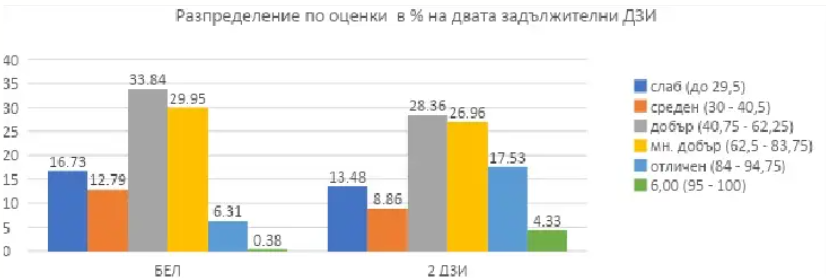
\includegraphics[width=1\textwidth]{diagram (1).png} 
\end{figure}

\vspace{0.6cm}

\noindent
\textbf{14. Защо според Текст 1 успехът на втория ДЗИ е по-висок? Посочете НЕВЕРНИЯ отговор.} \\
\noindent
\textbf{А)} Изпитът по БЕЛ е задължителен за всички зрелостници. \\
\textbf{Б)} На втория зрелостен изпит се явяват по-малко ученици. \\
\textbf{В)} Учениците, явяващи се на втория ДЗИ, са по-мотивирани. \\
\textbf{Г)} ДЗИ по БЕЛ е по-труден от останалите изпити.

\vspace{0.6cm}

\noindent
\textbf{15. Посочете НЕВЕРНИЯ отговор. Според Текст 1:} \\
\noindent
\textbf{А)} Няма зрелостник със 100 точки на двата изпита. \\
\textbf{Б)} Няма зрелостник с 0 т. на двата изпита. \\
\textbf{В)} Максимален брой точки на двата изпита имат 32 зрелостници. \\
\textbf{Г)} Две шестици имат 49 зрелостници.

\vspace{0.6cm}

\noindent
\textbf{16. Посочете НЕВЕРНИЯ отговор. Според диаграмата:} \\
\noindent
\textbf{А)} На ДЗИ по БЕЛ 33.84 \% са получили оценка Добър (40.75 -- 62.25 т.). \\
\textbf{Б)} Отличните оценки на втория държавен изпит са с 11.22 \% повече от отличните оценки на изпита по БЕЛ. \\
\textbf{В)} Преобладаващата част от зрелостниците имат оценки Среден и Добър на двата изпита. \\
\textbf{Г)} Оценка Отличен 6.00 (95 -- 100 т.) на ДЗИ по БЕЛ са получили 0.38 \% от зрелостниците.

\vspace{0.6cm}

\noindent
\textbf{17. Посочете НЕВЕРНИЯ отговор. Според Текст 1 и Текст 2:} \\
\noindent
\textbf{А)} Две слаби оценки (до 29.5 т.) имат 941 зрелостници. \\
\textbf{Б)} Две отлични оценки (84 -- 94.5 т.) имат 1651 зрелостници. \\
\textbf{В)} От всички зрелостници, явили се на ДЗИ по БЕЛ (43 011), оценка 6.00 (95 -- 100 т.) имат само 0.38 \% \\
\textbf{Г)} Само 1651 зрелостници имат две отлични оценки (84 -- 94.5 т.).

\vspace{0.6cm}

\noindent
\textbf{18. Според Текст 1 средният резултат на зрелостниците на втория задължителен изпит по математика е 69.19 т. Запишете каква оценка имат зрелостниците според диаграмата?}

\vspace{0.6cm}

\noindent
\textbf{19. Като имате предвид информацията от двата текста, запишете колко точки НЕ достигат на зрелостниците, за да имат оценка Мн. добър на втория зрелостен изпит.}

\vspace{0.6cm}

\noindent
\textbf{20. Запишете СЪС СВОИ ДУМИ защо зрелостниците имат по-нисък среден успех на ДЗИ по БЕЛ?}

\vspace{0.6cm}

\noindent
\textbf{21. Като имате предвид информацията от Текст 1, коментирайте в текст до 5 изречения следното:}

\begin{itemize}
    \item[\textendash] \textbf{Защо зрелостниците имат по-висок успех на втория ДЗИ?}
    \item[\textendash] \textbf{Как си обяснявате факта, че средно най-много точки зрелостниците имат на ДЗИ по чужд език?}
    \item[\textendash] \textbf{Защо зрелостниците имат висок среден успех на ДЗИ по математика?}
\end{itemize}

\newpage

\vspace{0.6cm}

\noindent
\textbf{ЧАСТ 2 (време за работа: 60 минути)}

\vspace{0.3cm}

\noindent
\underline{\textit{Отговорите на задачите от 22. до 40. включително отбелязвайте в листа за отговори.}}

\vspace{0.6cm}

\noindent
\textbf{22. В листа за отговори запишете само паронима, с който да поправите лексикалната грешка в изречението.} \\[0.3em]
\noindent
Обращението към публиката бе написано прочувствено.

\vspace{0.6cm}

\noindent
\textbf{23. За всяко празно място изберете УМЕСТНАТА дума и я запишете срещу съответната буква в листа за отговори.} \\[0.5em]
\noindent
Елин Пелин променя из основи жанра на разказа в българската литература. В разказите на Елин Пелин огромна роля за изграждането на художествените внушения играе \dots \textbf{(А)}. Той не е просто \dots \textbf{(Б)}, той е \dots \textbf{(В)} на събитието.

\vspace{0.4cm}

\noindent
\textbf{А)} пейзажът, случката, диалогът \\
\textbf{Б)} среда, фон, заден план \\
\textbf{В)} основата, сърцевината, душата

\vspace{0.6cm}

\noindent
\textbf{24. Какви са измерения на родното и чуждото за героите? Посочете НЕВЯРНОТО твърдение.} \\
\noindent
\textbf{А)} За Султана чуждо е всичко, което може да й попречи да укрепи и да въздигне западналия си род. \\
\textbf{Б)} За Лазар родното се свързва не само със семейно-родовата общност, то включва и понятията \textit{народ} и \textit{родина}. \\
\textbf{В)} За Рафе Клинче своето е творчеството, красотата и любовта. \\
\textbf{Г)} Родният свят за Стоян Глаушев е представен в романтична светлина.

\vspace{0.6cm}

\noindent
\textbf{25. Кой от проблемите е интерпретиран и в двата посочени откъса?} \\[0.5em]
\noindent
\textit{От днеска нататък българският род} \\
\textit{история има и става народ! (Ив. Вазов, "Паисий")} \\[0.5em]
\textit{Но разкажи със думи прости} \\
\textit{на тях -- на бъдещите хора,} \\
\textit{които ще поемат поста ни} \\
\textit{че ние храбро сме се борили. (Н. Вапцаров, "История")} \\[0.6cm]
\noindent
\textbf{А)} за написаната история като средство за самопознанието на нацията \\
\textbf{Б)} за историята като средство за духовното извисяване на българите \\
\textbf{В)} за написаната история като форма на колективната памет \\
\textbf{Г)} за гордостта на човека от историята

\vspace{0.6cm}

\noindent
\textbf{26. Кой от мотивите НЕ е интерпретиран в \textit{"Новото гробище над Сливница"}?} \\[0.3em]
\noindent
\textbf{А)} за героичната смърт, която осмисля човешкото съществуване \\
\textbf{Б)} за песента като прослава, в която се сливат човешкото и природното \\
\textbf{В)} за забравата и паметта \\
\textbf{Г)} за преходността на човешкото битие

\vspace{0.6cm}

\noindent
\textbf{27. Кое твърдение НЕ е вярно?} \\
\noindent
\textbf{А)} Анафоричното повторение на израза \textit{Сега съм у дома} в началото на всяка от осемте строфи на Вазовата ода \textit{"При Рилския манастир"} разкрива величието на природата. \\
\textbf{Б)} Ботев изгражда в стихотворението \textit{"Борба"} образа на един свят на преобърнатите ценности, като специална роля в това отношение играят оксимороните (\textit{лъжи святи, свещена глупост\dots}). \\
\textbf{В)} Двойната употреба на епитета \textit{бурлив} в стихотворението на Вазов \textit{"Новото гробище над Сливница"} внушава идеята, че човекът, извисен в битката за родината, се приближава до величавостта на природата. \\
\textbf{Г)} Инверсираното тавтологично словосъчетание \textit{ниви глухо опустели} показва трагичната самота на човека в Яворовата поема \textit{"Градушка"}.

\vspace{0.6cm}

\noindent
\textbf{28. Посочете значенията на паратекста (заглавието и епиграфа).} \\[0.5em]
\begin{flushright}
    \textit{"Приказка за стълбата"} \\
    \textit{Посветено на всички, които ще кажат:} \\
    \textit{Това не се отнася до мене!}
\end{flushright}
\vspace{0.4cm}
\noindent
\textbf{А)} Думата \textit{приказка} в заглавието насочва към представата за иносказание, фантазия. \\
\textbf{Б)} Думата \textit{стълба} в заглавието подсказва идеята за изкачване, за слизане. \\
\textbf{В)} Епиграфът (мотото) е предупреждение за всички, изкачващи се по стълбата на властта с цената на непростими нравствени компромиси, но отказващи да се разпознаят в героя на текста. \\
\textbf{Г)} В паратекста е зададен проблемът за обществото и властта, който ще се интерпретира в текста.

\vspace{0.6cm}

\noindent
\textbf{29. Кое от твърденията за пейзажа в Елин-Пелиновия разказ \textit{"Андрешко"} НЕ е вярно?} \\[0.5em]
\noindent
\textit{Земята тънеше в кал и влага. Мъртви и покрусени се тъмнееха пръснатите пейзажи на села, речища, далечни гори и планини. По полето лъщяха големи локви, мътни, студени и оцъклени като мъртвешки очи.} \\[0.6cm]
\noindent
\textbf{А)} Пейзажът е мрачен, потискащ, изпълнен с вариации на мъртвото и безизходното. \\
\textbf{Б)} Значенията на водата, която символизира обновлението, са преобърнати. \\
\textbf{В)} Мотивът за калта също носи внушения за безнадеждност и предопределеност. \\
\textbf{Г)} Мъртвата вода и неизбродимата кал подсказват, че героите са затънали в безчовечността.

\vspace{0.6cm}

\noindent
\textbf{30. Кое от твърденията НЕ е вярно?} \\
\noindent
\textbf{А)} Природата в одата \textit{"При Рилския манастир"} е възприета като храм на човешката душа, докато в поемата \textit{"Градушка"} човекът е безпомощен и обречен пред немилостивото лице на природата. \\
\textbf{Б)} Човекът е самотен в съзиданието и страданието, но в миниатюрата \textit{"Спи езерото"} (за разлика от поемата \textit{"Градушка"}) самотата е съзнателен избор, начин да се достигне самовглъбяване. \\
\textbf{В)} Природният кръговрат в одата \textit{"При Рилския манастир"} е символ на вечността, а в миниатюрата \textit{"Спи езерото"} -- на безвремието. \\
\textbf{Г)} Съзерцанието е път към духовната същност на живота и в одата \textit{"При Рилския манастир"}, и в поемата \textit{"Градушка"}.

\vspace{0.6cm}

\noindent
\textbf{31. Сходни моменти в изображението на родното, на балканските нрави има в:} \\
\noindent
\textbf{А)} \textit{"Железният светилник"} и \textit{"Бай Ганьо журналист"} \\
\textbf{Б)} \textit{"Бай Ганьо журналист"} и \textit{"Балкански синдром"} \\
\textbf{В)} \textit{"Балкански синдром"} и \textit{"При Рилския манастир"} \\
\textbf{Г)} \textit{"При Рилския манастир"} и \textit{"Новото гробище над Сливница"}

\vspace{0.6cm}

\noindent
\textbf{32. Кой герой от \textit{"Крадецът на праскови"} претърпява най-сериозно вътрешно развитие?} \\[0.4em]
\noindent
\textbf{А)} полковникът \hspace{1.5cm} \textbf{Б)} Елисавета \hspace{1.5cm} \textbf{В)} младият разказвач \hspace{1.5cm} \textbf{Г)} Иво

\vspace{0.6cm}

\noindent
\textbf{33. Посочете НЕВЯРНОТО твърдение} \\
\noindent
\textbf{А)} Историята на любовта между Елисавета и Иво е видяна през две различни гледни точки. \\
\textbf{Б)} Първият разказвач въвежда читателя в общата атмосфера на действието (наблюдението и спомените от живота на града по време на двете световни войни. \\
\textbf{В)} Вторият разказвач е учителят. \\
\textbf{Г)} Всевиждащият разказвач е необходим, за да може авторът да разграничи свидетелската от всевиждащата гледна точка.

\vspace{0.6cm}

\noindent
\textbf{34. Коя тема НЕ е интерпретирана в откъса от стихотворението на Иван Вазов \textit{"Към природата"}?} \\[0.5em]
\noindent
\textit{Поклон на теб, природо, създанье необятно} \\
\textit{на твоя свод лазурен, на твойто слънце златно,} \\
\textit{на твойта вечна младост и вечна красота,} \\
\textit{на всичко, що е в тебе божествено и тайно,} \\
\textit{невидимо, кат бога, велико и безкрайно} \\
\textit{и равно с вечността;} \\[0.6cm]
\noindent
\textbf{А)} за природата като дом \\
\textbf{Б)} за природната хармония \\
\textbf{В)} за природата като носител на божествения промисъл \\
\textbf{Г)} за природата като коректив на обществото

\vspace{0.6cm}

\noindent
\textbf{35. Съпоставете интерпретациите на темата за природата в \textit{"При Рилския манастир"} (\textit{"Към природата"}) и в \textit{"Градушка"} и запишете ЕДНА разлика в тях в листа за отговори.}

\vspace{0.6cm}

\noindent
\textbf{36. В листа за отговори разтълкувайте заглавието \textit{"Железният светилник"} в контекста на творбата.}

\vspace{0.6cm}

\noindent
\textbf{37. В листа за отговори посочете двете значения на думата \textit{история} в стихотворението \textit{"История"}.}

\vspace{0.6cm}

\noindent
\textbf{38. В листа за отговори запишете ЕДНА характерна черта за жанра на одата, проявена в \textit{"Паисий"}.}

\vspace{0.6cm}

\noindent
\textbf{39. Свържете заглавието на всяка от творбите с нейния автор. В листа за отговори срещу съответната буква запишете цифрата, съответстваща на името на автора.} \\[0.8em]
\begin{minipage}[t]{0.45\textwidth}
    \textbf{А)} \textit{"Ноев ковчег"} \\
    \textbf{Б)} \textit{"Балкански синдром"} \\
    \textbf{В)} \textit{"Спи езерото"}
\end{minipage}
\begin{minipage}[t]{0.45\textwidth}
    1. Пенчо Славейков \\
    2. Йордан Радичков \\
    3. Станислав Стратиев
\end{minipage}

\vspace{0.6cm}

\vspace{0.8cm}

\noindent
\textbf{40. В текст до 5 изречения съпоставете интерпретациите на темата за невъзможния диалог между народ и държава в посочените откъси.} \\[0.5em]

 
\indent Земеделецът, който едно време кажи-речи дивееше щастливо и в хамбара му се намираше от ново до ново, сега дояжда до Коледа и как се чеше по врата край кофтора в механата, говори: „Тежко се живее!“ И наистина е тежко: кръчмарят иска, лихварят иска, попът иска, касата иска, бирникът иска, за къща трябва\dots{} А пък тая пуста пара от нийде не иде. Нито работа има, ни печал има. Ако се опита да открадне една кола дърва от гората, за да вземе някой и друг грош за тях, ето че горският му съставя акт, дето се казва, че тоя човек нарушил член еди-кой си от закона за горите, как отсякъл в еди-коя си държавна гора толко и толко дървета с такава и такава дебелина, и затова му се пада такава и такава глоба\dots{} Па защо и какво е сякъл, това никой не пита. (\textit{Елин Пелин, "За едни майка, за други мащеха"}) \\[0.4em]
 
\indent По изпълнение, разбира се. Играе ме един вашенец там, ама тоя път ще му дам да разбере. Няколко пъти го гоня, а все се изплъзва от ръцете ми\dots{} Разбрах, че дяволува, и ще го издебна довечера, та ще ме помни\dots{} Житцето му ще секвестирам! Хем него на ум ще науча, хем да ви покажа един пример, та да не кръшкате друг път. Лъжете търговците, лъжете гражданите, та им продавате развалени яйца и граниво масло. Е, ама чакай, жено селяшка -- властта се лесно не лъже! Пипа тя -- здраво пипа! За вас камшик, руски камшик -- така ще се оправите\dots{} Станахте пияници, пропаднахте, развалихте се -- ще станете неспособни данъкоплатци и ще съсипете държавата. Ах, защо нямам повечечко власт! Ангели ще ви направя. (\textit{Елин Пелин, "Андрешко"})

\newpage

\noindent
\textbf{ЧАСТ 3 (Време за работа: 20 минути)}

\vspace{0.3cm}

\noindent
\underline{\textit{Не пречертавайте цялата таблица, ако не принтирате варианта. Номерирайте редовете}}

\vspace{0.6cm}

\noindent
\textbf{41. Попълнете пропуснатото в таблицата.}

\vspace{0.3cm}

\noindent
\renewcommand{\arraystretch}{1.8}
\begin{tabularx}{\textwidth}{|>{\raggedright\arraybackslash}X|>{\raggedright\arraybackslash}X|>{\raggedright\arraybackslash}X|>{\raggedright\arraybackslash}X|}
\hline
\hfil\bfseries Автор & \hfil\bfseries Произведение & \hfil\bfseries Жанр & \hfil\bfseries Герой \\ \hline
 &  & роман & Аврам Немтур \\ \hline
Емилиян Станев &  &  & ординарецът \\ \hline
 & „Андрешко“ &  & съдия-изпълнителят \\ \hline
 & „Бай Ганьо журналист“ &  & Гуньо Адвокатина \\ \hline
Христо Смирненски &  & разказ, притча &  \\ \hline
\end{tabularx}

\vspace{0.3cm}

\noindent
\renewcommand{\arraystretch}{1.8}
\begin{tabularx}{\textwidth}{|>{\raggedright\arraybackslash}X|>{\raggedright\arraybackslash}X|>{\raggedright\arraybackslash}X|>{\raggedright\arraybackslash}X|}
\hline
\hfil\bfseries Автор & \hfil\bfseries Тема & \hfil\bfseries Произведение & \hfil\bfseries Жанр \\ \hline
 & Природата &  & лирическа миниатюра \\ \hline
Иван Вазов &  & „Паисий“ &  \\ \hline
 &  & „Балкански & комедия на абсурда \\ 
 &  & синдром“ &  \\ \hline
Христо Ботев & Обществото и &  &  \\ 
 & властта &  &  \\ \hline
Емилиян &  &  & повест \\ 
Станев &  &  &  \\ \hline
\end{tabularx}

\newpage
\subsection{Тест върху "Железният светилник" и правописна норма}
\noindent
\textit{Име и фамилия:} \dotfill \textit{№} \makebox[2cm]{\dotfill}

\vspace{0.6cm}

\begin{center}
    {\large\bfseries Тест върху "Железният светилник" и правописна норма}
\end{center}

\vspace{0.6cm}

\noindent
\textbf{Част 1 (време за работа: 60 минути)}

\vspace{0.3cm}

\noindent
\underline{\textit{Отговорите на задачите от 1. до 21. включително отбелязвайте в листа за отговори.}}

\vspace{0.5cm}

\noindent
\textbf{1. В коя от думите има правописна грешка?} \\
\noindent
\textbf{А)} инженер \\
\textbf{Б)} акомулатор \\
\textbf{В)} тирбушон \\
\textbf{Г)} пеницилин

\vspace{0.6cm}

\noindent
\textbf{2. В кой ред НЕ е допусната правописна грешка?} \\
\noindent
\textbf{А)} манисто, астма, бастун \\
\textbf{Б)} бодър, разпра, огризение \\
\textbf{В)} влакче, прекупувам, заводски \\
\textbf{Г)} мързелив, неосетно, овощни

\vspace{0.6cm}

\noindent
\textbf{3. В кое от изреченията е допусната правописна грешка?} \\
\noindent
\textbf{А)} По образование и квалификация фелшерът е между лекаря и медицинската сестра. \\
\textbf{Б)} Агенцията по вписванията издаде методически указания за работата на длъжностните лица по регистрацията. \\
\textbf{В)} Уестминстърското абатство е посещавано всяка година от над милион туристи. \\
\textbf{Г)} Повечето известни писатели са били хора със сложен характер, с богата душевност и интересна съдба.

\vspace{0.6cm}

\noindent
\textbf{4. В кое от изреченията е допусната правописна грешка?} \\
\noindent
\textbf{А)} Титулярът на сметките, по които са получавани преводи от чужбина, е български гражданин. \\
\textbf{Б)} Букварът е част от цялостен учебен комплект по български език и литература за 1. клас по новата учебна програма. \\
\textbf{В)} Формулярът за кандидатстване за неимигрантска виза трябва да бъде попълнен изцяло. \\
\textbf{Г)} Съединителят представлява връзката между скоростната кутия и двигателя, преди да е натиснат педалът.

\vspace{0.6cm}

\noindent
\textbf{5. В кое от изреченията НЕ е допусната правописна грешка?} \\
\noindent
\textbf{А)} Статията разглежда спецификите и параметрите на употреба на понятията „имидж“, „репутация“ и „бранд“. \\
\textbf{Б)} Лудата гонидба на върха продължи стремглаво и в 26-ия кръг на английското футболно първенство. \\
\textbf{В)} Рупите е защитена местност, която е разположена на около 10 км от Петрич и на 2 км от с. Рупите. \\
\textbf{Г)}От около две години стоките на куфърните търговии, които редовно пътуват между България и Турция, се обмитяват.

\vspace{0.6cm}

\noindent
\textbf{5. В кое от изреченията НЕ е допусната правописна грешка?} \\
\noindent
\textbf{А)} Статията разглежда спецификите и параметрите на употреба на понятията „имидж“, „репутация“ и „бранд“. \\
\textbf{Б)} Лудата гонидба на върха продължи стремглаво и в 26-ия кръг на английското футболно първенство. \\
\textbf{В)} Рупите е защитена местност, която е разположена на около 10 км от Петрич и на 2 км от с. Рупите. \\
\textbf{Г)}От около две години стоките на куфърните търговии, които редовно пътуват между България и Турция, се обмитяват.

\vspace{0.6cm}

\noindent
\textbf{6. В коя от подчертаните думи е допусната правописна грешка?} \\
\noindent
\underline{\textbf{Информираността}} \textbf{(А)} относно Европа и европейската парламентарна демокрация, която осигурява Програмата за училища \underline{\textbf{посланици}} \textbf{(Б)} на Европейския парламент, цели да превърне младите хора в активни европейски граждани и да ги \underline{\textbf{насарчи}} \textbf{(В)} да участват в различни \underline{\textbf{инициативи}} \textbf{(Г)} на местно и международно ниво.

\vspace{0.6cm}

\noindent
\textbf{7. Открийте и поправете четиринайсетте правописни грешки в текста.} \\
\noindent
През 1879 година в северната часть на Испания любителят архиолог маркис Де Саутуола, придружен от четиригодишната си дъщеря, решил да разгледа пещерата Алтамира. Малката палълница явно не се интересувала от фкаменелостите, вълнуващи бащата. Но в пещерата имало няколко ниски галерии, които никой оважаващ себе си архиолог не би изследвал и където можело приятно да се поиграе. Детето пропалзяло в долната част на пещерата, носейки свещицата си. Но когато пугледнало към тавана, за най-голям негов ужас, одгоре се изблещили очите на угромен нарисуван бик. Оказало се, че стените и таваните на тези ниски галерии били покрити с прекрасни рисунки, дело на парвобитния човек.

\vspace{0.6cm}

\noindent
\textbf{8. В коя от думите е допусната правописна грешка?} \\
\noindent
\textbf{А)} колониален \\
\textbf{Б)} остта \\
\textbf{В)} влекат \\
\textbf{Г)} целостта

\vspace{0.6cm}

\noindent
\textbf{9. В коя от думите НЕ е допусната правописна грешка?} \\
\noindent
\textbf{А)} гръкът \\
\textbf{Б)} глобалистски \\
\textbf{В)} радиятор \\
\textbf{Г)} бактерия

\vspace{0.6cm}

\noindent
\textbf{10. В кое от изреченията е допусната правописна грешка?} \\
\noindent
\textbf{А)} Котките обичат чистотата и непрестанно се ближат, за да поддържат телата си чисти, както ги е научила еволюциата. \\
\textbf{Б)} Смята се, че малката гънка в края на котешкото ухо, образуваща продълговата вдлъбнатинка, изпълнява функцията на резонатор. \\
\textbf{В)} Котаракът Мирон пътешествал с геолози из платото Устюрт и самоотвержено охранявал лагера на експедицията от отровни змии. \\
\textbf{Г)} Днес котката е сред малкото бозайници, които могат да живеят с нас и в тесния, малък апартамент.

\vspace{0.6cm}

\noindent
\textbf{11. В кой ред е допусната правописна грешка?} \\
\noindent
\textbf{А)} министър на туризма \\
\textbf{Б)} цар Борис Трети \\
\textbf{В)} Столична Община \\
\textbf{Г)} хардрок

\vspace{0.6cm}

\noindent
\textbf{12. В кое от изреченията е допусната правописна грешка?} \\
\noindent
\textbf{А)} От древните летописци научаваме, че Александър Велики пренесъл за пръв път папагалите в Европа. \\
\textbf{Б)} На галапагоските острови живеят над двайсет животински вида, намиращи се под закрила, сред които е и морската игуана. \\
\textbf{В)} Котката в Древен Египет била не само свещено животно, но и ловец на гризачи, а също така и воин. \\
\textbf{Г)} От Египет домашната котка попаднала в Индия, Югоизточна Азия и Южна Европа.

\vspace{0.6cm}

\noindent
\textbf{13. В кое от изреченията НЕ е допусната правописна грешка?} \\
\noindent
\textbf{А)} Плиний Стари твърди, че страните на изтока са първите, в които се употребявали ароматни вещества. \\
\textbf{Б)} В древния Рим козмети се наричали робините, които се грижели за красотата на римлянките. \\
\textbf{В)} В средните векове само по време на църковна служба свещеници кадели тамян и помазвали вярващите с миро. \\
\textbf{Г)} През 1608 година монаси от доминиканския орден основали в манастир близо до Флоренция първата „парфюмерийна фабрика“.

\vspace{0.6cm}

\noindent
\textbf{14. В кое от изреченията е допусната правописна грешка?} \\
\noindent
\textbf{А)} Излагането на слънце през лятото не е опасно, ако спазваме съветите на лекарите. \\
\textbf{Б)} В Средна и Южна Европа август е един от най-хубавите месеци и плажовете са пълни с летовници. \\
\textbf{В)} Понякога ледът на повърхността на Северния Ледовит океан достига през зимата до три метра дебелина. \\
\textbf{Г)} Със застудяването на времето се укриват и редица други животни, които прекарват зимата в летаргичен сън.

\vspace{0.6cm}

\noindent
\textbf{15. В коя от подчертаните думи е допусната правописна грешка?} \\
\noindent
Декораторите обръщали особено внимание на камбаната и гребена на шлема. Заедно с изкованите сцени от \underline{\textbf{Античността}} \textbf{(А)}, \underline{\textbf{инкрустираните}} \textbf{(Б)} със злато или сребро \underline{\textbf{Ренесансови}} \textbf{(В)} мотиви гравирането било един от предпочитаните начини за \underline{\textbf{украсяване}} \textbf{(Г)}.

\vspace{0.6cm}

\noindent
\textbf{16. В коя от подчертаните думи НЕ е допусната правописна грешка?} \\
\noindent
Нова Зеландия, която се намира в югозападната част на Тихия \underline{\textbf{океан}} \textbf{(А)}, е островна държава, като по-голямата част от \underline{\textbf{територията}} \textbf{(Б)} й \underline{\textbf{опхваща}} \textbf{(В)} двата острова, наречени Северен и Южен, разделени от \underline{\textbf{Протока}} \textbf{(Г)} Кук.

\vspace{0.7cm}

\noindent
\textbf{18. В коя от думите има правописна грешка?} \\
\noindent
\textbf{А)} автокъща \\
\textbf{Б)} акваспининг \\
\textbf{В)} жълто-кафяв \\
\textbf{Г)} прахосмукачка-робот

\vspace{0.6cm}

\noindent
\textbf{18. В кой ред е допусната правописна грешка?} \\
\noindent
\textbf{А)} аутокю, астроном любител, закононарушение \\
\textbf{Б)} Дон-Кихотов, кънтри-певец, ландшафт \\
\textbf{В)} културтрегер, културно-просветен, родословие \\
\textbf{Г)} токшоу, помощник-готвач, кафе пауза

\vspace{0.6cm}

\noindent
\textbf{19. В кой ред НЕ е допусната правописна грешка?} \\
\noindent
\textbf{А)} кафе-сладкарница, ПИН-код, екопътека \\
\textbf{Б)} младши лейтенант, лироепически, килокалории \\
\textbf{В)} криотерапия, хипер инфлация, геолого-географски \\
\textbf{Г)} тупа-лупа, високоблагородие, жената котка

\vspace{0.6cm}

\noindent
\textbf{20. В коя от подчертаните думи е допусната правописна грешка?} \\
\noindent
Насекомите са били сред първите животни, които „са излезли от морето, отърсили са се от калта и са се добили с криле“, казва американският \underline{\textbf{ентомолог}} \textbf{(А)} Кати Прудич. Те произвеждат смайващо на брой поколение -- например мравките от вида Dorylus gribodoi снасят \underline{\textbf{три-четири}} \textbf{(Б)} милиона яйца на всеки 28 дни. \\
Малките същества разполагат и със завидни защитни оръжия: от \underline{\textbf{супер-твърдата}} \textbf{(В)} обвивка на някои бръмбари до токсичните шипове на южния фланелен молец. \\
Насекомите правят огромна услуга на \underline{\textbf{земеделието}} \textbf{(Г)} и околната среда, като обработват и обогатяват почвата, разпръскват семена и опрашват количество растения, представляващо около една трета от храната, произвеждана в света.

\vspace{0.6cm}

\noindent
\textbf{21. В кое от изреченията е допусната правописна грешка?} \\
\noindent
\textbf{А)} Таджикистан започва изграждането на водноелектрическата централа „Рогун“ -- проект на стойност 3,9 милиарда долара. \\
\textbf{Б)} Какво трябва непременно да знаете, преди да започнете тренировки по кикбокс? \\
\textbf{В)} Наскоро бившият министър и негови съмишленици учредиха център за евро-атлантическа сигурност. \\
\textbf{Г)} Има ли разлика между сухите и полу-сухите вина освен по отношение на захарта, която съдържат?

\vspace{0.6cm}

\noindent
\textbf{22. В кое от изреченията НЕ е допусната правописна грешка?} \\
\noindent
\textbf{А)} Корупционен скандал, в който са замесени и чужди служби, тресе северно-македонската съдебна система. \\
\textbf{Б)} За производството на шперплат най-често се използват топола, бреза, липа и иглолистна дървесина. \\
\textbf{В)} Николай Бердяев е руски философ и публицист, един от основателите на т.нар. Руски философско-религиозен ренесанс. \\
\textbf{Г)} Невиждайки кръжащия орел, кокошката спокойно разхождаше пиленцата си.

\vspace{0.6cm}

\noindent
\textbf{23. В кое от изреченията е допусната правописна грешка?} \\
\noindent
\textbf{А)} Възложителят поставя изисквания за защита на информацията с конфиденциален характер. \\
\textbf{Б)} Изберете демонстрационен автомобил, регистрирайте се на сайта ни и си запишете час за тест драйв. \\
\textbf{В)} Доброто кръвообръщение е от съществено значение за здравето на сърцето и на целия организъм. \\
\textbf{Г)} За Романтизма и Модернизма ключова е идеята за разкриване на скритото, за манифестиране на невидимото.

\newpage

\vspace{0.6cm}

\noindent
\textbf{ЧАСТ 2 (време за работа: 60 минути)}

\vspace{0.3cm}

\noindent
\textbf{24. Как НЕ може да се определят романите на Димитър Талев?} \\
\noindent
\textbf{А)} като социално-психологически \\
\textbf{Б)} като представителни за възрожденската традиция \\
\textbf{В)} като принадлежащи към реалистичната традиция \\
\textbf{Г)} като исторически

\vspace{0.6cm}

\noindent
\textbf{25. Коя от особеностите НЕ е характерна за четирилогията на Димитър Талев?} \\
\noindent
\textbf{А)} Основната й тема е историческата съдба на Македония. \\
\textbf{Б)} Вписва се в „голямата лирическа вълна“ от 50-те години на 20. век. \\
\textbf{В)} Романите са публикувани от 1952 до 1966 г. \\
\textbf{Г)} Те се появяват в условията на политическа диктатура.

\vspace{0.6cm}

\noindent
\textbf{26. Коя от опозициите е водеща за идеята на „Железният светилник“?} \\
\noindent
\textbf{А)} мрак -- светлина \\
\textbf{Б)} робство -- свобода \\
\textbf{В)} село -- град \\
\textbf{Г)} материално -- духовно

\vspace{0.6cm}

\noindent
\textbf{27. Кое е вярното твърдение?} \\
\noindent
\textbf{А)} „Железният светилник“ е първата част от трилогията на Димитър Талев за българите в Македония. \\
\textbf{Б)} „Железният светилник“ е единствената творба на Талев с тема и герои от епохата на Възраждането. \\
\textbf{В)} Вазовият роман „Под игото“ е оказал силно емоционално влияние върху Димитър Талев. \\
\textbf{Г)} Действието в „Железният светилник“ се развива в град Прилеп по време на османското владичество.

\vspace{0.6cm}

\noindent
\textbf{28. Коя от опозициите НЕ се открива в романа „Железният светилник“?} \\
\noindent
\textbf{А)} родното -- чуждото \\
\textbf{Б)} селото -- градът \\
\textbf{В)} образованието -- трудът \\
\textbf{Г)} патриархалната норма -- индивидуалният избор

\vspace{0.6cm}

\noindent
\textbf{29. Кои са трите основни ценности, на които се уповава събуденото национално самосъзнание на българина в Талевия роман? Посочете НЕВЕРНИЯ отговор.} \\
\noindent
\textbf{А)} християнската вяра като сплотяваща етноса \\
\textbf{Б)} българският език като основен народностен маркер \\
\textbf{В)} просветата – събуждането на историческа памет и на чувство за родов дълг \\
\textbf{Г)} единението с братята гърци срещу турските поробители

\vspace{0.6cm}

\noindent
\textbf{30. Как Лазар Глаушев разбира мисията на народния водач? Посочете НЕВЯРНОТО твърдение.} \\
\noindent
\textbf{А)} като бягство от личните си терзания \\
\textbf{Б)} като отказ от следване на личния интерес в името на обществените задачи \\
\textbf{В)} като поемане на рискове в името на народната кауза \\
\textbf{Г)} като смелост в противопоставянето срещу гръцките духовници и фанариоти

\vspace{0.6cm}

\noindent
\textbf{31. Защо Султана избира Стоян за свой съпруг?} \\
\noindent
\textbf{А)} защото е влюбена в него \\
\textbf{Б)} защото вижда в него здрав и надежден стълб на своето бъдещо семейство \\
\textbf{В)} защото иска да направи напук на старата баба хаджийка \\
\textbf{Г)} защото смята старите патриархални норми и традиции за отживелица

\vspace{0.6cm}

\noindent
\textbf{32. Избройте четири промени в обществения живот в Преспа, които се осъществяват в хода на сюжета.} \\
\noindent
\makebox[\textwidth]{\dotfill} \\
\makebox[\textwidth]{\dotfill} \\
\makebox[\textwidth]{\dotfill} \\
\makebox[\textwidth]{\dotfill}

\vspace{0.6cm}

\noindent
\textbf{33. Кой от метафоричните образи, използвани от рилския духовник, е израз на стремежа на Султана да съхрани преди всичко семейството?} \\
\noindent
\textbf{А)} черупката, в която се опитваме да се скрием, без да подозираме, че „ще дойде черният гарван и ще я счупи с клюна си“ \\
\textbf{Б)} орелът, който лети към небето със свободни крила, „а нашите крила са сковани“ \\
\textbf{В)} българите като „широк залив от безбрежно славянско море“ \\
\textbf{Г)} овце, които гръцките фанариоти искат да смесят със своето стадо, за да стане по-силно

\vspace{0.6cm}

\noindent
\textbf{34. Каква НЕ е позицията на героя повествовател в „Железният светилник“?} \\
\noindent
\textbf{А)} Представя детайлно собствения си поток на съзнанието. \\
\textbf{Б)} Вижда героите обективно и построява техните характеристики. \\
\textbf{В)} Представя обществените събития и протичането на историята. \\
\textbf{Г)} Тази на класическия третоличен „вездесъщ“ повествовател.

\vspace{0.6cm}

\noindent
\textbf{35. За какво НЕ служи честата употреба на полупряка реч в романа „Железният светилник“?} \\
\noindent
\textbf{А)} Повествователят се доближава максимално до гледните точки на героите. \\
\textbf{Б)} Така се дава обяснение на скритите мотиви на героите. \\
\textbf{В)} Служи в някои случаи за иронично дистанциране от думите на героите. \\
\textbf{Г)} Дава се обяснение на значението на архаичните или диалектните думи.

\vspace{0.8cm}

\textit{Прочетете откъса от романа „Железният светилник“ и изпълнете задачите от 36. до 38. включително.}

\vspace{0.4cm}

\noindent
Малко по-късно Султана и Лазар останаха сами в голямата стая. \\
– Майко, какво става с Катерина? \\
Султана притвори очи, като да се замисли, или за миг се отдаде на умората си. \\
– Какво й е... Пометна. Кръвта не спира. \\
– Но, мамо... – викна Лазар с \underline{\textbf{пресекнал}} \textbf{(А)} глас, – трябва да направим нещо! Не може тъй да чакаме. Да вземем една кола, да я заведем в Битоля. Там има добри хекими. \\
– В Битоля... \underline{\textbf{Ако изтрае днеска...}} \textbf{(Б)} Като се пусне еднаж кръв, мъчно е да се спре. Сама може да спре, а Битоля е далеко. Ако не спре кръвта сама... \\
Лазар каза, без да погледне майка си: \\
– Защо направи това, майко? Щом било толкова опасно, да беше останало така най-сетне. Ето, Катерина може да загуби живота си. \\
– Да – въздъхна Султана, – може... Мислех си, толкова жени пометат. Знаех също, че и много жени затриват живота си. Ако Катерина умре, нека сени ми каже: ти я уби! Направих го, а пък аз й съм майка. Никого нема да боли повече от мене. Аз си знам колко ме боли и как се страхувам за живота й. Но и сега да трябва да почна – пак ще го направя. \\
Тя дигна към сина си остър, мрачен поглед: – Не искам моята щерка да роди копеле. Кой както иска, така да ме съди. \\
Тя се наведе над огнището, посбута огъня без нужда. Лазар мълчеше. Той не одобреваше постъпката на майка си, но \underline{\textbf{кой може да съди една майка за това, което върши за децата си, дори}} \underline{\textbf{и когато прави грешки}} \textbf{(В)}?

\vspace{0.8cm}

\noindent
\textbf{36. Със свои думи посочете три примера за грешките, които допуска Султана.} \\
\noindent
\makebox[\textwidth]{\dotfill} \\
\makebox[\textwidth]{\dotfill} \\
\makebox[\textwidth]{\dotfill} \\
\makebox[\textwidth]{\dotfill}

\vspace{0.6cm}

\noindent
\textbf{37. С цитати от речта на повествователя посочете четири примера, които доказват, че Талев е майстор на разгърнатите психологически характеристики на своите герои.} \\
\noindent
\makebox[\textwidth]{\dotfill} \\
\makebox[\textwidth]{\dotfill} \\
\makebox[\textwidth]{\dotfill} \\
\makebox[\textwidth]{\dotfill} \\
\makebox[\textwidth]{\dotfill} \\
\makebox[\textwidth]{\dotfill}

\vspace{0.6cm}

\noindent
\textbf{38. Срещу съответната буква запишете какви са подчертаните изразни средства в текста.} \\
\noindent
\textbf{А)} \makebox[0.8\textwidth]{\dotfill} \\
\textbf{Б)} \makebox[0.8\textwidth]{\dotfill} \\
\textbf{В)} \makebox[0.8\textwidth]{\dotfill}
\newpage
\subsection{Тест върху раздела Любовта и лексикална норма}
\noindent
\textit{Име и фамилия:} \dotfill \textit{№} \makebox[2cm]{\dotfill}

\vspace{0.6cm}

\begin{center}
    {\large\bfseries Тест върху раздела Любовта и лексикална норма}
\end{center}

\vspace{0.6cm}

\noindent
\textbf{Част 1 (време за работа: 60 минути)}

\vspace{0.3cm}

\noindent
\underline{\textit{Отговорите на задачите от 1. до 21. включително отбелязвайте в листа за отговори.}}

\vspace{0.5cm}

\noindent
\textbf{1. В кое изречение е допусната лексикална грешка?} \\
\noindent
\textbf{А)} Бях приключил с обидчивата си гордост; бях приключил с всичките си дребни прояви на суетност и високомерие. \\
\textbf{Б)} Отдавна вече мирската суета не го трогваше, беше съсредоточен в намеренията си, които превъзхождаха възможностите на човешката природа. \\
\textbf{В)} Сънят и вцепенението отстъпиха място на някакво необичайно трескаво и безсмислено суетене. \\
\textbf{Г)} Такива хора трудно признават собствените си грешки - не заради перфекционизъм, а от накърнена суетливост и самолюбие.

\vspace{0.6cm}

\noindent
\textbf{2. В кое изречение е допусната лексикална грешка?} \\
\noindent
\textbf{А)} Вилата е без текуща вода и без електричество. \\
\textbf{Б)} Той беше човек, завладян от фикс идеи, потаен и вероятно параноик. \\
\textbf{В)} Изчезнал без предизвестие - това бе професионалният евфемизъм за убит. \\
\textbf{Г)} Всеки от десетте отпечатъка на човешките пръсти е уникален.

\vspace{0.6cm}

\noindent
\textbf{3. В кое изречение е допусната лексикална грешка?} \\
\noindent
\textbf{А)} Свещените писания са истории и легенди за опитите на човек да разбере потребността си от смисъл на собственото си съществуване. \\
\textbf{Б)} В музея имаше малка папирусна книжка, изписана с чудновати писмена, които се извиваха като змии. \\
\textbf{В)} Без писменост историите били предавани от уста на уста и обикновено украсявани. \\
\textbf{Г)} Йероглифната писменост съчетава в себе си изобразителните елементи с абстрактните.

\vspace{0.6cm}

\noindent
\textbf{4. В кое изречение е допусната лексикална грешка?} \\
\noindent
\textbf{А)} Той се приближи още и започна да се взира в неясните букви. \\
\textbf{Б)} Родителите й бяха починали преди години и единственият й стожер сега беше баба й. \\
\textbf{В)} Неделният следобед е най-чудесното време за мързелуване, книги, филми и лежерни разговори. \\
\textbf{Г)} Той е стоял извън литературните разпри на своето време и сам е наричал себе си дилетант.

\vspace{0.6cm}

\noindent
\textbf{5. В кое изречение НЕ е допусната лексикална грешка?} \\
\noindent
\textbf{А)} Аз успях да предизвикам интересна дилема на тази тема, която за съжаление прерасна в спор и завърши с разправия. \\
\textbf{Б)} Поради авария ТЕЦ „Бобов дол“ спира част от мощите си за десетина дни. \\
\textbf{В)} Домакинът се разположи в едно кресло край масичката до прозореца и отправи нехаен жест към госта си. \\
\textbf{Г)} В подобни случаи полицията има право дори да използва параноичен газ за разпръскване на тълпата.

\vspace{0.6cm}

\noindent
\textbf{6. В кое изречение НЕ е допусната лексикална грешка?} \\
\noindent
\textbf{А)} Кариерата му на писател започва през 1865 г. и той приема литературния прякор Марк Твен, с който е известен като автор на „Приключенията на Том Сойер“. \\
\textbf{Б)} Познавам подробно брат си и мога да заявя с увереност, че той не е способен на подобна постъпка. \\
\textbf{В)} Той е изконен сърбин, роден е в Сърбия, майка му и баща му са сърби. \\
\textbf{Г)} Запалил се беше доста късно по стрелбата с лък, но упорстваше и дори се беше явявал на състезания за аматьори.

\vspace{0.6cm}

\noindent
\textbf{7. В кой ред фразеологичните словосъчетания НЕ са синоними?} \\
\noindent
\textbf{А)} дните ми са преброени - пътник съм \\
\textbf{Б)} замайва ми се главата - изгубвам си ума \\
\textbf{В)} на куков ден - на второ пришествие \\
\textbf{Г)} с ченгел му вадят думите - вързан в устата

\vspace{0.6cm}

\noindent
\textbf{8. В кой ред фразеологичните словосъчетания НЕ са синоними?} \\
\noindent
\textbf{А)} вземам ума - свалям звезди от небето \\
\textbf{Б)} ям душата - пека на шиш \\
\textbf{В)} отпускам му края - удрям го на живот \\
\textbf{Г)} имам редки пръсти - пара не свъртам

\vspace{0.6cm}

\noindent
\textbf{9. В кой ред фразеологичните словосъчетания са синоними?} \\
\noindent
\textbf{А)} не подвивам крак - не паса трева \\
\textbf{Б)} като куче и котка - между Сцила и Харибда \\
\textbf{В)} вятър ме вее на бял кон - вятър работа \\
\textbf{Г)} като две капки вода - одрал му е кожата

\vspace{0.6cm}

\noindent
\textbf{10. В кой ред фразеологичните словосъчетания са синоними?} \\
\noindent
\textbf{А)} опитно зайче - заешка душа \\
\textbf{Б)} вдигам ръце - дигам си парцалите \\
\textbf{В)} бабини деветини - врели-некипели \\
\textbf{Г)} чиста ми е работата - света вода ненапита

\vspace{0.6cm}

\noindent
\textbf{11. В кой ред фразеологичните словосъчетания са антоними?} \\
\noindent
\textbf{А)} работи му ченето - слага си катинар на устата \\
\textbf{Б)} вземам ума - изгубвам си ума \\
\textbf{В)} вземам за чиста монета - гледам накриво \\
\textbf{Г)} тупам се в гърдите - преминавам през огън и вода

\vspace{0.6cm}

\noindent
\textbf{12. В кой ред фразеологичните словосъчетания НЕ са антоними?} \\
\noindent
\textbf{А)} чета конско евангелие - пея осанна \\
\textbf{Б)} вързан съм в ръцете - имам лека ръка \\
\textbf{В)} галеник на съдбата - роден на черен петък \\
\textbf{Г)} ум като бръснач - с два пръста чело

\vspace{0.6cm}

\noindent
\textbf{13. В кой ред фразеологичните словосъчетания НЕ са антоними?} \\
\noindent
\textbf{А)} цепя косъма на две - имам широки пръсти \\
\textbf{Б)} като църковна мишка - като крез \\
\textbf{В)} плаша се от сянката си - не ми мигва окото \\
\textbf{Г)} в черна светлина - на бял свят

\vspace{0.8cm}

\noindent
\textbf{14. За всяко празно място изберете най-уместния от предложените изрази.} \\
\noindent
Всяка сериозна дискусия относно ролята на войната в човешките общества, и преди всичко дебатите за или против нейната неизбежност, \makebox[2cm]{\dotfill} (А) ни отправят към въпроса за нейния произход. Знайно е, че организираната война е неизменен спътник на цивилизацията още от началото на писаната история, но това все пак не са повече от пет хиляди години. Ако военни действия съществуват още преди цивилизацията, та дори и преди човека, то тогава \makebox[2cm]{\dotfill} (Б) тревожната вероятност войната да се окаже неизбежна част от нашето генетично наследство. Подобна мисъл би била действително \makebox[2cm]{\dotfill} (В), но въпреки това сме длъжни да й \makebox[2cm]{\dotfill} (Г) достатъчно внимание. \\
\noindent
\textbf{А)} наложително, фатално, неминуемо \\
\textbf{Б)} изниква, се ражда, се показва \\
\textbf{В)} умопомрачителна, обезкуражаваща, предизвикваща \\
\textbf{Г)} посветим, дадем, удостоим

\vspace{0.6cm}

\noindent
\textbf{15. За всяко празно място изберете най-уместния от предложените изрази.} \\
\noindent
Личните взаимоотношения са \makebox[2cm]{\dotfill} (А) за нас, както въздухът, който дишаме. Всички ние се нуждаем от приятели, любими, партньори, от хора, с които да \makebox[2cm]{\dotfill} (Б) радости, мъки, опасения и успехи. Това общуване \makebox[2cm]{\dotfill} (В) най-нежните ни струни и обогатява и най-затънтените кътчета на душата ни. Всички се нуждаем от дружба, любов, добра компания и чувство за принадлежност и въпреки това често оставаме на разстояние един от друг, не желаейки или не можейки да протегнем ръка и да \makebox[2cm]{\dotfill} (Г) пълноценен контакт. \\
\noindent
\textbf{А)} основополагащи, жизненоважни, изконни \\
\textbf{Б)} разменим, доверим, споделим \\
\textbf{В)} докосва, свири на, обтяга \\
\textbf{Г)} осъществим, правим, сътворим

\vspace{0.6cm}

\noindent
\textbf{16. За всяко празно място изберете най-уместния от предложените изрази.} \\
\noindent
Литературата \makebox[2cm]{\dotfill} (А) мисленето, разширява хоризонта, приучава към правенето на връзки и сравнения, набавя ориентация, защото не е тайна, че по литературата може да се направят изводи за обществата, каквито невинаги могат да се \makebox[2cm]{\dotfill} (Б) от документите. Всяко произведение предполага противоречивост, смътност, неопределеност и по този начин винаги е \makebox[2cm]{\dotfill} (В) за ума. Учителите трябва да се стремят да \makebox[2cm]{\dotfill} (Г) познавателно и изследователско любопитство. \\
\noindent
\textbf{А)} форсира, аргументира, стимулира \\
\textbf{Б)} измъкнат, експлоатират, извлекат \\
\textbf{В)} обстоятелство, предизвикателство, свидетелство \\
\textbf{Г)} култивират, активират, импулсират

\vspace{0.6cm}

\noindent
\textbf{17. За всяко празно място изберете най-уместния от предложените изрази.} \\
\noindent
Докато се разхождаме из приветливите коридори, младежи играят спокойно на карти, а момиченца скачат на въже в прекрасния вътрешен двор. Минаваме от стая в стая и навсякъде децата учат: в голямата и светла библиотека, в лъскавата компютърна зала или просто в класната стая. Откриваме същата \makebox[2cm]{\dotfill} (А) обстановка и в учителската стая, където също не липсват компютри. Но най-невероятното нещо е \makebox[2cm]{\dotfill} (Б) на шум. Защо тези деца не крещят? Защо например не използват отсъствието на учителя, за да се замерят с пергели? Все пак те са в тази особено \makebox[2cm]{\dotfill} (В) възраст. Както всички младежи в Европа, и те имат пиърсинг, качулки, които нахлупват чак до носа, и джинси, завлечени до колена. Само че \makebox[2cm]{\dotfill} (Г) спокойни. \\
\noindent
\textbf{А)} уютна, доброкачествена, китна \\
\textbf{Б)} дефицитът, недостигът, липсата \\
\textbf{В)} опасна, фатална, преломна \\
\textbf{Г)} напомнят на, изглеждат, стават

\vspace{0.6cm}

\noindent
\textbf{18. За всяко празно място изберете най-уместния от предложените изрази.} \\
\noindent
Бъдеще, настояще и минало за мен са части от едно безкрайно време, в него онова, което наричаме минало, за миг се превръща в настояще или бъдеще и обратно! Ако светът \makebox[2cm]{\dotfill} (А) по-добре миналото, вярвам, че много от сегашните \makebox[2cm]{\dotfill} (Б) биха изчезнали. Трябва да живеем заедно, \makebox[2cm]{\dotfill} (В) етическите, етническите, историческите, литературните \makebox[2cm]{\dotfill} (Г). Историята показва, че никой не може да живее сам, затова трябва да живеем заедно. \\
\noindent
\textbf{А)} предугаждаше, познаваше, долавяше \\
\textbf{Б)} перипетии, поразии, недоразумения \\
\textbf{В)} съзерцавайки, съзнавайки, съзирайки \\
\textbf{Г)} различия, варианти, несъответствия

\vspace{0.6cm}

\noindent
\textbf{19. За всяко празно място изберете най-уместния от предложените изрази.} \\
\noindent
Аз съм тази, която се усмихва първа \makebox[2cm]{\dotfill} (А) да съм мила и любезна и съответно ми се отговаря със същото. Държа се добре с всички, това работи и постепенно би могло да стане \makebox[2cm]{\dotfill} (Б) и на останалите. Въпрос на лично \makebox[2cm]{\dotfill} (В), което, разбира се, отнема време. Живели сме дълго време намусени и искаме рязко всичко да се смени, но това са сложни \makebox[2cm]{\dotfill} (Г) в психиката на човека – да свикне да съществува в тези нови условия, не е лесно. \\
\noindent
\textbf{А)} старая се, силя се, определям \\
\textbf{Б)} ритуал, традиция, навик \\
\textbf{В)} превъзнасяне, превъзпитание, превъплъщаване \\
\textbf{Г)} похвати, процеси, качества

\vspace{0.6cm}

\noindent
\textbf{20. За всяко празно място изберете най-уместния от предложените изрази.} \\
\noindent
Желанието на учителите да научат на много неща претоварва учениците - това е един от основните проблеми на образованието. По някои предмети учителите \makebox[2cm]{\dotfill} (А) прекалено много детайли дори и от учениците, които нямат намерение да се занимават в бъдеще с дадената наука. Така реално не се получават знания, а нещо се назубря временно, колкото да мине изпитването. Повечето ученици днес искат да виждат \makebox[2cm]{\dotfill} (Б) в това, което учат. \makebox[2cm]{\dotfill} (В) „трябва да го знаеш, защото утре ще те изпитам“ отдавна вече не работи. Днешните деца повече от всякога имат нужда от посока, от цели и \makebox[2cm]{\dotfill} (Г), които да им помогнат да ги постигнат. \\
\noindent
\textbf{А)} претендират за, налагат, изискват \\
\textbf{Б)} резултат, смисъл, поанта \\
\textbf{В)} аргументът, заповедта, доказателството \\
\textbf{Г)} претекст, привилегия, мотивация

\newpage

\vspace{0.6cm}

\noindent
\textbf{ЧАСТ 2 (време за работа: 60 минути)}

\vspace{0.3cm}

\noindent
\textbf{21. Кой от посочените факти НЕ е свързан със стихотворението на Димчо Дебелянов „Аз искам да те помня все така...“?} \\
\noindent
\textbf{А)} Творбата има кръгова композиция. \\
\textbf{Б)} Имало е посвещение: „На Зв.“. \\
\textbf{В)} Заглавието е цитатно. \\
\textbf{Г)} Първата публикация е в сп. „Родна реч“.

\vspace{0.6cm}

\noindent
\textbf{22. Посочете кой е жанрът на всяка от творбите.}  \\
\noindent
\begin{minipage}[t]{0.6\textwidth}
\textbf{А)} „Аз искам да те помня все така...“ на Димчо Дебелянов \\
\textbf{Б)} „Колко си хубава!“ на Христо Фотев \\
\textbf{В)} „Посвещение“ на Петя Дубарова
\end{minipage}
\begin{minipage}[t]{0.35\textwidth}
1. изповед \\
2. елегия \\
3. възхвала
\end{minipage}

\vspace{0.3cm}
\noindent
А -- \makebox[1cm]{\dotfill} \hspace{0.5cm} Б -- \makebox[1cm]{\dotfill} \hspace{0.5cm} В -- \makebox[1cm]{\dotfill}

\vspace{0.6cm}

\noindent
\textbf{23. Посочете основния мотив, чрез който е представена темата за любовта в стихотворението на Димчо Дебелянов „Аз искам да те помня все така...“.} \\
\noindent
\textbf{А)} печалния спомен \\
\textbf{Б)} възвишената красота \\
\textbf{В)} бленуваната хармония \\
\textbf{Г)} споделената обич

\vspace{0.6cm}

\noindent
\textbf{24. Посочете кое НЕ може да се отнесе към Дебеляновата творба „Аз искам да те помня все така...“.} \\
\noindent
\textbf{А)} невъзможното щастие в любовта \\
\textbf{Б)} тъгата по неизживения живот \\
\textbf{В)} тъжните слова на девойката \\
\textbf{Г)} драматичната раздяла с любимата

\vspace{0.6cm}

\noindent
\textbf{25. Какво замества местоимението \textit{Тя} в творбата „Аз искам да те помня все така...“?} \\
\noindent
\textbf{А)} любимата \\
\textbf{Б)} любовта \\
\textbf{В)} самотата \\
\textbf{Г)} смъртта

\vspace{0.6cm}

\noindent
\textbf{26. Посочете мотивите, които са свързани в стихотворението „Колко си хубава!“ на Христо Фотев.} \\
\noindent
\textbf{А)} красотата и любовта \\
\textbf{Б)} красотата и доброто \\
\textbf{В)} споменът и раздялата \\
\textbf{Г)} споменът и обичта

\vspace{0.6cm}

\noindent
\textbf{27. Кое художествено средство НЕ присъства в цитата от стихотворението „Колко си хубава!“ на Христо Фотев?} \\
\textit{Колко са хубави ръцете ти.} \\
\textit{И нозете ти колко са хубави.} \\
\textit{И очите ти колко са хубави.} \\
\textit{И косите ти колко са хубави.} \\
\noindent
\textbf{А)} реторично възклицание \\
\textbf{Б)} анафора \\
\textbf{В)} синтактичен паралелизъм \\
\textbf{Г)} метафора

\vspace{0.6cm}

\noindent
\textbf{28. Стиховете „в ръка ми вплела пламнала ръка“ са от стихотворението:} \\
\noindent
\textbf{А)} „Колко си хубава!“ на Христо Фотев \\
\textbf{Б)} „Посвещение“ на Петя Дубарова \\
\textbf{В)} „Аз искам да те помня все така...“ на Димчо Дебелянов \\
\textbf{Г)} „До моето първо либе“ на Христо Ботев

\vspace{0.6cm}

\noindent
\textbf{29. Кой мотив НЕ е свързан с темата за любовта в стихотворението на Христо Фотев „Колко си хубава!“?} \\
\noindent
\textbf{А)} красотата на любимата \\
\textbf{Б)} очарованието на спомена \\
\textbf{В)} въздействието на любовта \\
\textbf{Г)} възхищението на влюбения

\vspace{0.6cm}

\noindent
\textbf{30. Кое твърдение НЕ е вярно за стихотворението „Колко си хубава!“ на Христо Фотев?} \\
\noindent
\textbf{А)} Творбата е възхвала на женската красота. \\
\textbf{Б)} Образът на любимата е идеализиран. \\
\textbf{В)} Съкровеното желание на Аза е да опази любовта си. \\
\textbf{Г)} Първата публикация е в стихосбирката „Баладично пътуване“.

\vspace{0.6cm}

\noindent
\textbf{31. Посочете НЕВЯРНОТО.} \\
\textbf{Специфичният поетически ритъм в стихотворението на Христо Фотев „Колко си хубава!“ се постига чрез:} \\
\noindent
\textbf{А)} анафори \\
\textbf{Б)} епифори \\
\textbf{В)} синтактичен паралелизъм \\
\textbf{Г)} метонимии

\vspace{0.6cm}

\noindent
\textbf{32. Кой смислов акцент НЕ се съдържа в повторението „обичай ме!“ в стихотворението на Христо Фотев „Колко си хубава!“?} \\
\noindent
\textbf{А)} съкровен призив \\
\textbf{Б)} изповедна молба \\
\textbf{В)} магично заклинание \\
\textbf{Г)} настойчив спомен

\vspace{0.6cm}

\noindent
\textbf{33. Посочете художественото средство, което се открива в стиха „И да си зла – обичай ме!“ от стихотворението на Христо Фотев „Колко си хубава!“.}  \\
\noindent
\textbf{А)} антитеза \\
\textbf{Б)} смислов парадокс \\
\textbf{В)} градация \\
\textbf{Г)} оксиморон

\vspace{0.6cm}

\noindent
\textbf{34. В стихотворението „Посвещение“ на Петя Дубарова драматичните изживявания на лирическата героиня са изразени чрез антитези. Посочете НЕВЯРНАТА.} \\
\noindent
\textbf{А)} между самотата и любовта \\
\textbf{Б)} между страха и смелостта \\
\textbf{В)} между бляна и спомена \\
\textbf{Г)} между греха и светостта

\vspace{0.6cm}

\noindent
\textbf{35. Образът на лирическата героиня в „Посвещение“ на Петя Дубарова е свързан с:} \\
\noindent
\textbf{А)} изживяването на хармонията в силата на любовните чувства \\
\textbf{Б)} примирението с превратностите на съдбата \\
\textbf{В)} раздвоението между чувство за вина и желанието за свобода \\
\textbf{Г)} признанието за необратимия трагичен край на любовта

\vspace{0.6cm}

\noindent
\textbf{36. Какъв е идейният акцент във финалните стихове на „Посвещение“ на Петя Дубарова?}  \\
\noindent
\textbf{А)} духовен порив за свобода \\
\textbf{Б)} мечта за духовна хармония \\
\textbf{В)} копнеж за духовно съзряване \\
\textbf{Г)} романтичен блян за любимия

\vspace{0.6cm}

\noindent
\textbf{37. Посочете НЕВЯРНОТО.} \\
\textbf{Основната идея, изразена чрез оксиморона в стиха „а в свойта вяра сам не вярвам аз“ от стихотворението на Димчо Дебелянов „Аз искам да те помня все така...“ е за:} \\
\noindent
\textbf{А)} раздялата на човека с надеждата \\
\textbf{Б)} липсата на ценностен ориентир \\
\textbf{В)} безсилието на човека пред съдбата \\
\textbf{Г)} вечното човешко страдание

\vspace{0.6cm}

\noindent
\textbf{38. Коментирайте в рамките на 4 – 5 изречения внушенията на стиховете „и любовта ни сякаш по е свята, / защото трябва да се разделим“ от стихотворението на Димчо Дебелянов „Аз искам да те помня все така...“.} \\
\noindent
\makebox[\textwidth]{\dotfill} \\
\makebox[\textwidth]{\dotfill} \\
\makebox[\textwidth]{\dotfill} \\
\makebox[\textwidth]{\dotfill} \\
\makebox[\textwidth]{\dotfill}

\vspace{0.6cm}

\noindent
\textbf{39. Разтълкувайте в рамките на 3 – 4 изречения символиката на луната в стихотворението „Посвещение“ на Петя Дубарова.} \\
\noindent
\makebox[\textwidth]{\dotfill} \\
\makebox[\textwidth]{\dotfill} \\
\makebox[\textwidth]{\dotfill} \\
\makebox[\textwidth]{\dotfill}

\vspace{0.6cm}

\noindent
\textbf{40. Напишете теза за есе върху стихотворението на Христо Фотев „Колко си хубава!“ на тема „Любовта – истина за смисъла на човешкото битие“.} \\
\noindent
\makebox[\textwidth]{\dotfill} \\
\makebox[\textwidth]{\dotfill} \\
\makebox[\textwidth]{\dotfill} \\
\makebox[\textwidth]{\dotfill} \\
\makebox[\textwidth]{\dotfill}
\newpage

\subsection{ОБОБЩИТЕЛЕН ТЕСТ КЪМ ДЯЛ 1 „ЛЮБОВТА“}
\noindent
\textit{Име и фамилия:} \dotfill \textit{№} \makebox[2cm]{\dotfill}

\vspace{0.6cm}

\begin{center}
{\large\bfseries ТЕСТ 4} \\
{\bfseries ОБОБЩИТЕЛЕН ТЕСТ КЪМ ДЯЛ 1 „ЛЮБОВТА“}
\end{center}

\vspace{0.5cm}

\noindent
\textbf{1. В кой от редовете \textbf{НЕ} е допусната правописна грешка?} \\
\textbf{А)} разложка, стоношка, нишка \\
\textbf{Б)} медийна, стадии, поразий \\
\textbf{В)} невинаги, навярно, незнаейки \\
\textbf{Г)} повърхностни, тягостни, безнадеждни

\vspace{0.6cm}

\noindent
\textbf{2. В кое от изреченията \textbf{НЕ} е допусната правописна грешка?} \\
\textbf{А)} Пожарникарът, който спасява света, е герой от роман, определен за бестселър № 1 за 2016 г. \\
\textbf{Б)} Повечето Троянски коне се стремят да откраднат с цел финансова печалба. \\
\textbf{В)} Познавам ги от дете и двете – майката е известна пианистка, а дъщеря й е виолончелистка. \\
\textbf{Г)} Тя е израснала в музикално семейство и затова още от малка свири виртуозно на цигулка.

\vspace{0.6cm}

\noindent
\textbf{3. В кое от изреченията \textbf{НЕ} е допусната граматична грешка при членуването?} \\
\textbf{А)} Каза ми, че през зимния сезон жълтите и червени ябълки са най-подходящи за диетата ми. \\
\textbf{Б)} Участвам с голям ентусиазъм в дарителската кампания на Университет по библиотекознание и информационни технологии. \\
\textbf{В)} Времето е най-безпристрастният съдник на събитията в човешката история, на делата и приноса на големите личности за благото на хората. \\
\textbf{Г)} Васил Иванов Кунчев, Апостолът на свободата, е един от идеолозите на българската национална революция.

\vspace{0.6cm}

\noindent
\textbf{4. В кое от изреченията \textbf{Е} допусната граматична грешка?} \\
\textbf{А)} Сали Яшар осъзнава силата на неговите харуци да носят радост и щастие в света, изпълнен с мъки и нещастия. \\
\textbf{Б)} Типичен пример за нравствен катарзис е разказът „Индже“, който поставя проблема за осъзнаване на жизнената цел на човека. \\
\textbf{В)} Очаквам и се надявам на вашето положително отношение към този проект, защото е свързан с развитието на общината. \\
\textbf{Г)} Би Би Си съобщават, че ще намалят разходите за уебсайта си с 25\% още другия месец, като въведат някои подобрения.

\vspace{0.6cm}

\noindent
\textbf{5. В кое от изреченията \textbf{НЕ} е допусната пунктуационна грешка?} \\
\textbf{А)} Няколко парчета диня, кората от 1 лимон, 3/4 ч. ч. лимонов сок, 1/2 ч. ч. светъл мед и един лимон на резени за украса, са достатъчни да подготвите освежаващата лимонада. \\
\textbf{Б)} Благодарение на усилията на по-заможни и просветени възрожденци, по време на Българското възраждане работят над 130 читалища. \\
\textbf{В)} В днешно време, често се говори за миграцията като личен избор, от една страна, и като спешна необходимост, от друга. \\
\textbf{Г)} Именно чрез събудената съвест човешкото съществуване придобива истински смисъл според В. Франкъл.

\vspace{0.6cm}

\noindent
\textbf{6. В кое от изреченията е допусната пунктуационна грешка?} \\
\textbf{А)} Мисълта с какво мога да допринеса на света, не ми даваше покой през всичките тези години. \\
\textbf{Б)} Тя е наясно, че, за да успее, трябва да я възприемат като уверена и безкомпромисна. \\
\textbf{В)} Припомних си мъдростта на Андерсен: „Можеш да видиш истинския облик на планината само когато се отдалечиш от нея“. \\
\textbf{Г)} Естествено, вярвам й, защото винаги е искрена с мен, а в трудни моменти е на първа линия.

\vspace{0.6cm}

\noindent
\textbf{7. Коя двойка фразеологични словосъчетания \textbf{НЕ} са синоними?} \\
\textbf{А)} от дън душа – от все сърце \\
\textbf{Б)} стоя в сянка – в глуха линия съм \\
\textbf{В)} между нас казано – между Сцила и Харибда \\
\textbf{Г)} хвърлям зад гърба си – махвам с ръка

\vspace{0.6cm}

\noindent
\textbf{8. От коя творба е посоченият откъс?} \\
Ела! Ще измиєм луната от грях! \\
Ще хвърлим трупа на умрелия страх, \\
ще пеем с тъмнежния корабен глас \\
на морската нощ във добрия Бургас. \\

\vspace{-0.1cm}

\noindent
\begin{minipage}[t]{0.48\textwidth}
    \textbf{А)} „Две хубави очи“\\[0.5em]
    \textbf{Б)} „Аз искам да те помня все така“
\end{minipage}%
\begin{minipage}[t]{0.48\textwidth}
    \textbf{В)} „Колко си хубава!“\\[0.5em]
    \textbf{Г)} Посвещение
\end{minipage}

\vspace{0.6cm}

\noindent
\textbf{9. Кое от посочените твърдения \textbf{НЕ} е вярно за междутекстовия диалог на „Аз искам да те помня все така“, „Колко си хубава!“ и „Посвещение“?} \\
\textbf{А)} И трите стихотворения са създадени през годините, в които властва комунистическата идеология, а любовната тема не е сред престижните в литературата. \\
\textbf{Б)} „Аз искам да те помня все така“ на Димчо Дебелянов е различна от другите творби като настроение и в жанрово отношение. \\
\textbf{В)} И към трите лирически произведения има посвещения, но трите посвещения имат различно значение за разбирането на творбите. \\
\textbf{Г)} И в трите творби лирическите герои се обръщат към любимия човек и внушават съкровена интимност на споделените чувства.

\vspace{0.6cm}

\noindent
\textbf{10. Кое е характерно за съотнасянето на любовта с времето в трите творби? Посочете \textbf{НЕВЯРНОТО} твърдение.} \\
\textbf{А)} Само една от творбите разкрива моменти от миналото на обичания човек. \\
\textbf{Б)} В Дебеляновата творба любовта е представена като спомен в настоящето. \\
\textbf{В)} Според лирическата героиня на Петя Дубарова любовта ще стане реалност в бъдещето. \\
\textbf{Г)} Според героя на Фотев любовта е силна само в мига на настоящето, а бъдещето е несигурно.

\vspace{0.6cm}

\noindent
\textbf{11. В коя от творбите „Аз искам да те помня все така“, „Колко си хубава!“ и „Посвещение“ присъстват повелителни глаголни форми като израз на императивност на посланието или като молба?} \\

\vspace{-0.1cm}

\noindent
\begin{tabular}{@{}p{0.48\textwidth} p{0.48\textwidth}@{}}
\textbf{А)} „Аз искам да те помня все така“ & \textbf{В)} „Посвещение“ \\
\textbf{Б)} във всяка от изброените & \textbf{Г)} в нито една от изброените
\end{tabular}

\vspace{0.6cm}

\noindent
\textbf{12. В коя творба любовта е изцяло духовна и протича в призрачна символистична атмосфера?} \\

\vspace{-0.1cm}

\noindent
\begin{tabular}{@{}p{0.48\textwidth} p{0.48\textwidth}@{}}
\textbf{А)} „Посвещение“ & \textbf{В)} „Аз искам да те помня все така“ \\
\textbf{Б)} „Колко си хубава!“ & \textbf{Г)} в нито една от изброените
\end{tabular}

\vspace{0.6cm}

\noindent
\textbf{13. В коя от посочените двойки творби образът на нощта \textbf{НЕ} се свързва единствено със страха и самотата?} \\

\vspace{-0.1cm}

\noindent
\begin{tabular}{@{}p{0.58\textwidth} p{0.58\textwidth}@{}}
\textbf{А)} „Посвещение“ и „Колко си хубава!“ & \textbf{В)} „Посвещение“ и „В часа на синята мъгла“ \\
\textbf{Б)} „Аз искам да те помня все така“ и „Колко си хубава!“ & \textbf{Г)} във всички посочени двойки
\end{tabular}

\vspace{0.6cm}

\noindent
\textbf{14. Коя от творбите е написана в бели стихове?} \\

\vspace{-0.1cm}

\noindent
\begin{tabular}{@{}p{0.48\textwidth} p{0.48\textwidth}@{}}
\textbf{А)} „Аз искам да те помня все така“ & \textbf{В)} „Посвещение“ \\
\textbf{Б)} „Колко си хубава!“ & \textbf{Г)} всички посочени творби
\end{tabular}

\vspace{0.6cm}

\noindent
\textbf{15. Трима ученици разискват образа на мъжа в трите текста. Изберете това твърдение, което съвпада с вашата гледна точка, и посочете 2 аргумента, за да го защитите.}

\vspace{0.3cm}

\noindent
\begin{tabularx}{\linewidth}{|>{\centering\arraybackslash}X|>{\centering\arraybackslash}X|>{\centering\arraybackslash}X|}
\hline
Образът на мъжа е различен в трите творби. & В „Посвещение“ и „Колко си хубава“ образът на мъжа има общи черти. & Образът на мъжа има общи черти в трите творби. \\
\hline
\end{tabularx}

\vspace{0.4cm}

\noindent
\textbf{Аргументи:} \\
\noindent\rule{\linewidth}{0.4pt}
\noindent\rule{\linewidth}{0.4pt}
\noindent\rule{\linewidth}{0.4pt}
\noindent\rule{\linewidth}{0.4pt}
\noindent\rule{\linewidth}{0.4pt}
\noindent\rule{\linewidth}{0.4pt}
\noindent\rule{\linewidth}{0.4pt}
\noindent\rule{\linewidth}{0.4pt}
\noindent\rule{\linewidth}{0.4pt}
\noindent\rule{\linewidth}{0.4pt}
\noindent\rule{\linewidth}{0.4pt}
\noindent\rule{\linewidth}{0.4pt}

\vspace{0.6cm}

\noindent
\textbf{Прочетете двата текста и изпълнете задачи 16 – 23.}

\vspace{0.4cm}

\noindent
\textbf{Текст 1} \\
В Южно Мароко има вихрушка, гаджеж, от която фелахите се защитават с ножове. Вятърът африко е достигнал понякога до Рим. Алм е есенен, идващ от Югославия. А арифи, или ареф, или рифи, изпепелява всичко по пътя си с хиляди огнени езици. Това са постоянни ветрове, които живеят в сегашно време.

Има и други, непостоянни, дето сменят посоката си, събират конете си и се обръщат срещу движението на часовниковата стрелка. Бист роз върлува сто седемдесет и седем дни в Афганистан, поми-буря, която преоблича всичко в яркожълто и си отива, последвана от дъжд. Харматан духа, докато издуха и себе си в Атлантическия океан. Имбат е морски бриз от Северна Африка. Има ветрове, които само въздишат към небето. Има нощни пясъчни бури, които носят студа със себе си. [...] Дату идва откъм Гибралтар и донася ухания.

Познат е и тайният вятър на пустинята. Неговото име било завинаги заличено от владетеля, чийто син попаднал във вихъра му и там намерил гибелта си. Нафхат е силен вятър от Арабия. Бешабар е чер и сух, „черен вятър“, и идва от североизток, от Кавказ.

\vspace{0.2cm}
\hfill \textit{Из „Английският пациент“ от М. Ондатджи}

\vspace{0.4cm}

\noindent
\textbf{Текст 2} \\
Четири човешки събии насред ужасите на Втората световна война. Сплотени от болката и желанието за оцеляване. Събрани от съдбата и войната и спасени от любовта.

През 1992 г. Майкъл Ондатджи публикува романа „Английският пациент“. В творбата писателят успява да събере четири човешки съдби на хора, наранени от Втората световна война. Действието се развива в Италия – в изолирана тосканска вила в края на 1944 и началото на 1945 г. Романът е изграден основно върху две сюжетни линии и те се пресичат в „английския пациент“ – човек, който е обезорал до неузнаваемост. Първата разказва за любовта на английския пациент – унгарския граф Алмаси. Той изследва либийската пустиня и има връзка с Катрин Клифтън – съпругата на друг изследовател.

Втората сюжетна линия разказва за Хана – двайсетгодишна канадецка медицинска сестра, която се грижи за обегорелия от самолетна катастрофа и умиращ пациент. По-късно към тях се присъединяват Караваджо – крадец, шпионин, измъчван и осакатен от военнопрестъпници, приятел на баща ѝ, и Кип – млад сикх и салчър, който през деня разчиства района от немски бомби и мини, а през нощта е с Хана.

Алмаси е наречен „английският пациент“, тъй като документите за самоличността му са загубени, когато катастрофира със самолета си в северноафриканската пустиня. Обезорял много лошо, той е спасен от бедуини. Не може да си спомни кой е, но е лекуван като британски офицер. Причините са, че говори английски и очевидно е с високо социално положение.

Романът е носител на наградата „Букър“ за 1992 г. През 1996 г. по книгата е заснет и едноименен филм с участието на Ралф Файнс, Кристин Скот Томас и Жулиет Бинош. Филмът е отличен с две награди „Златен глобус“ и девет награди „Оскар“.

\vspace{0.2cm}
\hfill \textit{Из интернет}

\vspace{0.6cm}

\noindent
\textbf{16. Каква функция изпълнява Текст 1?} \\
\textbf{А)} Посочва конкретното мястото и времето на действие в романа. \\
\textbf{Б)} Пресъздава експресивно духа на пустинята чрез ветровете в нея. \\
\textbf{В)} Констатира последиците от ветровете в африканската пустиня. \\
\textbf{Г)} Представя научна информация за метеорологичните условия в Африка.

\vspace{0.6cm}

\noindent
\textbf{17. Използваният в Текст 1 израз „които живеят в сегашно време“ е употребен със значението:} \\
\textbf{А)} които не се употребяват с други глаголни времена \\
\textbf{Б)} които в бъдещето се изгубват без следа \\
\textbf{В)} които никога не престават \\
\textbf{Г)} които непрекъснато се променят

\vspace{0.6cm}

\noindent
\textbf{18. Кое от посочените твърдения е вярно според Текст 1?} \\
\textbf{А)} Представени са два вида ветрове – постоянни и непостоянни. \\
\textbf{Б)} Ветровете имат по едно име, а само един вятър няма име. \\
\textbf{В)} Ветровете създават само проблеми за хората. \\
\textbf{Г)} Ветровете не могат да прекосяват континентите.

\vspace{0.6cm}

\noindent
\textbf{19. В коя сфера на общуване се използва Текст 2?} \\

\vspace{-0.1cm}

\noindent
\begin{tabular}{@{}p{0.48\textwidth} p{0.48\textwidth}@{}}
\textbf{А)} в битовата сфера & \textbf{В)} в научната сфера \\
\textbf{Б)} в естетическата сфера & \textbf{Г)} в медийната сфера
\end{tabular}

\vspace{0.6cm}

\noindent
\textbf{20. Кое от посочените твърдения се отнася за Текст 2?} \\

\vspace{-0.1cm}

\noindent
\begin{tabular}{@{}p{0.48\textwidth} p{0.48\textwidth}@{}}
\textbf{А)} Текстът представлява реклама с апелативна функция. & \textbf{В)} Текстът е изчерпателен и емоционално въздействащ. \\
\textbf{Б)} Текстът включва кратко резюме на книгата. & \textbf{Г)} Текстът е оформен стандартизирано.
\end{tabular}

\vspace{0.6cm}

\noindent
\textbf{21. Запишете буквите САМО на онези 4 факта, които НЕ присъстват в Текст 1 и Текст 2.} \\
\textbf{А)} Суданската пясъчна буря е в жълти цветове и е последвана от дъжд. \\
\textbf{Б)} Ветровете са назовани със своите имена, които ги идентифицират. \\
\textbf{В)} Хабуб е горещ сух вятър от Тунис, който изостря нервите. \\
\textbf{Г)} Ветровете, които въздишат към небето, са много слаби. \\
\textbf{Д)} Основната сюжетна линия в романа на Ондатджи е за любовта на Алмаси и Хана. \\
\textbf{Е)} Хана – двайсетгодишната медицинска сестра, се грижи за умиращия пациент в Канада. \\
\textbf{Ж)} В Мароко има вихрушка, от която местните се отбраняват с оръжие. \\
\textbf{З)} Караваджо е шпионин, осакатен от военнопрестъпници, приятел на Алмаси.

\vspace{0.6cm}

\noindent
\textbf{22. Относно това дали Текст 1 е подходящ откъс, който може да се добави към анотацията на романа „Английският пациент“ (Текст 2), двама ученици изказват различно мнение.} \\
\textit{Първо мнение:} Напълно подходящ – интригуващо описание! \\
\textit{Второ мнение:} Не мисля, че е подходящ – по-скоро обърква читателя!

\vspace{0.2cm}
\noindent
\textbf{Изберете една от позициите и я защитете с 2 аргумента.}

\vspace{0.3cm}
\noindent\rule{\linewidth}{0.4pt}
\noindent\rule{\linewidth}{0.4pt}
\noindent\rule{\linewidth}{0.4pt}
\noindent\rule{\linewidth}{0.4pt}
\noindent\rule{\linewidth}{0.4pt}
\noindent\rule{\linewidth}{0.4pt}
\noindent\rule{\linewidth}{0.4pt}
\noindent\rule{\linewidth}{0.4pt}
\noindent\rule{\linewidth}{0.4pt}
\noindent\rule{\linewidth}{0.4pt}

\vspace{0.6cm}

\noindent
\textbf{23. В рамките на 3–4 изречения формулирайте СОБСТВЕНА теза на тема \textit{Името и неговата сила}.}

\vspace{0.3cm}
\noindent\rule{\linewidth}{0.4pt}
\noindent\rule{\linewidth}{0.4pt}
\noindent\rule{\linewidth}{0.4pt}
\noindent\rule{\linewidth}{0.4pt}
\noindent\rule{\linewidth}{0.4pt}
\noindent\rule{\linewidth}{0.4pt}
\noindent\rule{\linewidth}{0.4pt}
\noindent\rule{\linewidth}{0.4pt}
\noindent\rule{\linewidth}{0.4pt}
\noindent\rule{\linewidth}{0.4pt}

\vspace{0.6cm}

\noindent
\textbf{24. Запишете правилните форми на думите, поставени в скоби.} \\
\textbf{А) Членуване} \\
(Проект) \dotfill на Постановление на (Министерски) \dotfill съвет за приемане на \\
Устройствен правилник на Агенция „Митници“ бе дискутиран продължително. \\
С първите лъчи на слънцето той откри невероятна гледка в (пустош) \dotfill. \\
Ето го (учебник) \dotfill по който се готвих за изпита.

\vspace{0.4cm}

\noindent
\textbf{Б) Местоимения} \\
Няма да чакам (никой/никого) \dotfill повече, защото достатъчно се забавихме. \\
Той беше упорит състезател, (чийто/чиито) \dotfill победи ме възхищаваха. \\
Тя ме впечатли не толкова със зашеметяващата си фигура, колкото с магията на (нейните/своите) \dotfill очи.

\vspace{0.4cm}

\noindent
\textbf{В) Учтива форма} \\
Госпожо, ако сте (бил) \dotfill (щастлив) \dotfill тук, бихте ли се (върнал) \dotfill отново при нас?

\vspace{0.6cm}

\noindent
\textbf{25. Препишете текста, като редактирате допуснатите 6 грешки.} \\
Поетът с ватенката, певецът на новото време – нито едно от тези популярни определения не е точно за човека
Пеньо Пенев, нито едно от тях не разкрива дълбоката му душевна драма, житейските сътресения, трагизмът и обреченоста му. Той е сред най-известните ни поети от първото следвоенно поколение творци. Днес обаче малцина знаят
Пеньо Пеневата поема Дни на проверка само защото се отнася към едно друго време – към зората на тоталитарното
строителство.

\vspace{0.3cm}
\noindent\rule{\linewidth}{0.4pt}
\noindent\rule{\linewidth}{0.4pt}
\noindent\rule{\linewidth}{0.4pt}
\noindent\rule{\linewidth}{0.4pt}
\noindent\rule{\linewidth}{0.4pt}
\noindent\rule{\linewidth}{0.4pt}
\noindent\rule{\linewidth}{0.4pt}
\noindent\rule{\linewidth}{0.4pt}
\noindent\rule{\linewidth}{0.4pt}
\noindent\rule{\linewidth}{0.4pt}
\noindent\rule{\linewidth}{0.4pt}
\noindent\rule{\linewidth}{0.4pt}

\vspace{0.6cm}

\noindent
\textbf{Прочетете откъсите от творбите и изпълнете задачи 26 – 30.}

\vspace{0.3cm}

\noindent
\begin{tabularx}{\linewidth}{|>{\raggedright\arraybackslash}X|>{\raggedright\arraybackslash}X|}
\hline
\textbf{„Аз искам да те помня все така“} & \textbf{„Колко си хубава!“} \\
\hline
А все по-страшно пада нощ над нас, & Не ме изгубвай никога – откривай ме, \\
чертаят мрежа прилепите в мрака, & изпълвай ме с детинско изумление. \\
утеха сетна твоята немощ чака, & Отново да се уверя в ръцете ти, \\
а в своята вяра сам не вярвам аз. \textbf{(А)} & В нозете ти, в очите ти... Обичай ме! \\
И ти отпущаш пламнала ръка & Как искам да те задържа завинаги. \\
и тръгваш, поглед в тъмнината впила, & Да ме обичам завинаги – \\
изгубила дори за сълзи сила. – & завинаги. \\
Аз искам да те помня все така... & И колко ми е невъзможно... \textbf{(Б)} Колко си \\
& ти пясъчна... И моля те, не казвай ми, \\
& че искаш да ме задържиш завинаги, \\
& да ме обичаш завинаги, \\
& завинаги. \\
\hline
\end{tabularx}

\vspace{0.6cm}

\noindent
\textbf{26. Запишете 3 образа или мотива, които присъстват и в двата откъса.}\\
\noindent\rule{\linewidth}{0.4pt}
\noindent\rule{\linewidth}{0.4pt}
\noindent\rule{\linewidth}{0.4pt}
\noindent\rule{\linewidth}{0.4pt}
\noindent\rule{\linewidth}{0.4pt}
\noindent\rule{\linewidth}{0.4pt}
\noindent\rule{\linewidth}{0.4pt}
\noindent\rule{\linewidth}{0.4pt}
\noindent\rule{\linewidth}{0.4pt}

\vspace{0.6cm}

\noindent
\textbf{27. Със СВОИ ДУМИ посочете 2 примера, които подкрепят твърдението, че в двата откъса мотивът за раздялата е интерпретиран по различен начин.} \\
\noindent\rule{\linewidth}{0.4pt}
\noindent\rule{\linewidth}{0.4pt}
\noindent\rule{\linewidth}{0.4pt}
\noindent\rule{\linewidth}{0.4pt}
\noindent\rule{\linewidth}{0.4pt}
\noindent\rule{\linewidth}{0.4pt}
\noindent\rule{\linewidth}{0.4pt}
\noindent\rule{\linewidth}{0.4pt}
\noindent\rule{\linewidth}{0.4pt}
\noindent\rule{\linewidth}{0.4pt}

\vspace{0.6cm}

\noindent
\textbf{28. Каква е функцията на образа на ръката/ръцете в двата текста? Посочете 2 примера.} \\
\noindent\rule{\linewidth}{0.4pt}
\noindent\rule{\linewidth}{0.4pt}
\noindent\rule{\linewidth}{0.4pt}
\noindent\rule{\linewidth}{0.4pt}
\noindent\rule{\linewidth}{0.4pt}
\noindent\rule{\linewidth}{0.4pt}
\noindent\rule{\linewidth}{0.4pt}
\noindent\rule{\linewidth}{0.4pt}

\vspace{0.6cm}

\noindent
\textbf{29. Каква е функцията на образа на очите/погледа в двата текста? Посочете 2 примера.}\\
\noindent\rule{\linewidth}{0.4pt}
\noindent\rule{\linewidth}{0.4pt}
\noindent\rule{\linewidth}{0.4pt}
\noindent\rule{\linewidth}{0.4pt}
\noindent\rule{\linewidth}{0.4pt}
\noindent\rule{\linewidth}{0.4pt}
\noindent\rule{\linewidth}{0.4pt}
\noindent\rule{\linewidth}{0.4pt}

\vspace{0.6cm}

\noindent
\textbf{30. Определете какви са подчертаните изразни средства в откъсите, и разтълкувайте техния смисъл.} \\
\textbf{А)} \dotfill
\vspace{0.2cm}
\noindent\rule{\linewidth}{0.4pt}
\noindent\rule{\linewidth}{0.4pt}
\noindent\rule{\linewidth}{0.4pt}

\vspace{0.3cm}

\noindent
\textbf{Б)} \dotfill
\vspace{0.2cm}
\noindent\rule{\linewidth}{0.4pt}
\noindent\rule{\linewidth}{0.4pt}
\noindent\rule{\linewidth}{0.4pt}

\vspace{0.6cm}

\noindent
\textbf{31. Коментирайте в 3 – 4 изречения следния цитат: „Изтрива имената! Изтрива националностите! Това беше духът на пустинята“ (Майкъл Ондатджи), като имате предвид цитираните в теста и изучените художествени творби.}\\

\noindent\rule{\linewidth}{0.4pt}
\noindent\rule{\linewidth}{0.4pt}
\noindent\rule{\linewidth}{0.4pt}
\noindent\rule{\linewidth}{0.4pt}
\noindent\rule{\linewidth}{0.4pt}
\noindent\rule{\linewidth}{0.4pt}
\noindent\rule{\linewidth}{0.4pt}
\noindent\rule{\linewidth}{0.4pt}
\noindent\rule{\linewidth}{0.4pt}

\newpage

\subsection{ТЕСТ 5}

\noindent
\textit{Име и фамилия:} \dotfill \textit{№} \makebox[2cm]{\dotfill}

\vspace{0.6cm}

\begin{center}
{\large\bfseries ТЕСТ 5}
\end{center}

\vspace{0.3cm}

\noindent
\textbf{І МОДУЛ}

\vspace{0.2cm}

\noindent
\textbf{Прочетете двата текста и изпълнете задачите към тях (от 1. до 5. включително).}

\vspace{0.6cm}

\noindent
\textbf{ТЕКСТ 1} \\
Има дни, в които не мога да пиша. Има цели седмици, в които не мога да пиша. Това нямаше да е такъв проблем, ако можех предварително да определя кои ще са тези дни и седмици. Щях да намаля щетите и да поема на маратон по Темза. Или пък да хвана влака за обиколка по галериите... Но за съжаление, разбирам, че един ден е такъв, когато по обяд осъзнавам, че съм се взирал с часове в празния екран. Или съм драскал някаква тежка, неубедителна проза, която трябва да изтрия след това.

Мисля, че проблемът е в това, че не съм ужасно добър писател. Но съм много хладнокръвен и прецизен редактор (който по стечение на обстоятелствата е женен за дори по-добър редактор). Освен това съм безцеремонен, когато трябва да изтрия някакъв слаб текст. Всъщност трия поне три четвърти от това, което пиша. Прецеждам и прецеждам. И някъде между версии номер 15 и 25 нещо се случва. Стигам дотам, че когато четеш собствените си думи, вече имаш чувство, че някой друг ги е писал...

Понякога, когато не се чувствам много уверен, прекарвам сутрини, работейки в някое квартално кафене. Тълпата ме накара да се чувствам като част от света на заетите хора. В такива моменти препрочитам написаното в предишните дни, полирам, изразявам отново себе си.

Писането е като правене на операция или като пилотиране – трябва да работят всички тилиндри. Иначе ще се наложи да правиш нещо друго. Затова, когато усетя, че не става, се прибирам у дома, пускам пералнята, рисувам или просто правя крос по Темза.

Не мисля, че бих могъл да пиша, ако не чувах заглушено в главата си онзи глас, който ми казва пак и пак: „Това не е достатъчно добро... Пиши повече, пиши по-добре... Време лети“.

\vspace{0.2cm}
\hfill \textit{Марк Хадън, автор на „Странна куче с куче през нощта“, „Петното“ и „Червената къща“}

\vspace{0.6cm}

\noindent
\textbf{ТЕКСТ 2} \\
Какво друго е истинският автор на фрагменти освен човек, способен да обобщи частица от световния порядък в една-едничка мисъл. Колкото по-близо стига до едничката мисъл, толкова е по-достоен за похвала. И би бил съвършен, ако попада винаги в центъра на завършения и концентриран изказ. Гледна точка, от която собствената ми работа върху тази книга с фрагменти ме разочарова.

Аз губя много време, много място там, където би трябвало да оставя само категоричен знак; думите ми не са способни да обхванат енергията, изстреляна от съзнанието в залп, да изградят от нея ясна и съвсем прибрана звукова и смислова постройка. Достатъчно е да оня, който познава истинската сила на думите – една безкрайна тайна, – да си послужи с пет или шест от тях: слънцето изгрява, защото великолепието му е обяснено, а е възможно и да ни затиснат тъмни грамади, пороища и страх. Вярно е, десеторно повече думи биха могли да кажат същото, но и с десет пъти по-малка сила.

В странни посоки може да те отведе такова чувство на вина. Откриеш ли идеята си (върху която, без съмнение, ще се разпростре ненужно), отхрувисто и блестящо изложена у друг, преминаваща високо над главите като звуци от сребърен тромпет, ти си готов да останеш с вдигнати очи и да благодариш. Понесла те е люлката на разума, изплетена така отдавна за човечеството; собствената ти мисъл е поднесена вече съвършено и ти се чувстваш свободен от голяма грижа. Чувстваш се закрилян, ученик, дете...

Днешният човек, уж пестелив към времето си, уж галопиращ през живота, е забравил (именно защото галопира) що е истински размисъл и концентрация. Точно затова е многословен.

\vspace{0.2cm}
\hfill \textit{Димитър Коруджиев, „Болката, когато е прекрасна“}

\vspace{0.6cm}

\noindent
\textbf{1. Кое от посочените твърдения НЕ се отнася до Текст 1?} \\
\textbf{А)} За да пише добре, един писател се нуждае от разговор със своята съвест. \\
\textbf{Б)} Писателят често е твърде критичен към текстовете, които смята за слаби. \\
\textbf{В)} Когато чете свои произведения, творецът усеща, че у него се пробужда силно вдъхновение. \\
\textbf{Г)} Ако можеш да предвидиш ефективността на творческата работа, писателят би имал време и за други занимания.

\vspace{0.6cm}

\noindent
\textbf{2. Защо според Текст 2 съвременният човек трудно може да оформи мисълта си в синтезиран вид?} \\
\textbf{А)} Защото изпитва огорчение, че други преди него вече са развили неговите идеи. \\
\textbf{Б)} Защото динамиката на живота е променила способността му за концентрация. \\
\textbf{В)} Защото е загубил детската си непосредственост и спонтанност на изказа. \\
\textbf{Г)} Защото е изгубил способността си да познава истинската сила на думите.

\vspace{0.6cm}

\noindent
\textbf{3. Обяснете защо според Текст 1 писането е като правене на операция или пилотиране.}
\noindent\rule{\linewidth}{0.4pt}
\noindent\rule{\linewidth}{0.4pt}
\noindent\rule{\linewidth}{0.4pt}
\noindent\rule{\linewidth}{0.4pt}
\noindent\rule{\linewidth}{0.4pt}
\noindent\rule{\linewidth}{0.4pt}
\noindent\rule{\linewidth}{0.4pt}
\noindent\rule{\linewidth}{0.4pt}

\vspace{0.6cm}

\noindent
\textbf{4. Като имате предвид информацията в Текст 1 и Текст 2, запишете ДВА аргумента в подкрепа на твърдението, че процесът на писане изисква от твореца да бъде критичен и взискателен към себе си.}
\noindent\rule{\linewidth}{0.4pt}
\noindent\rule{\linewidth}{0.4pt}
\noindent\rule{\linewidth}{0.4pt}
\noindent\rule{\linewidth}{0.4pt}
\noindent\rule{\linewidth}{0.4pt}
\noindent\rule{\linewidth}{0.4pt}
\noindent\rule{\linewidth}{0.4pt}
\noindent\rule{\linewidth}{0.4pt}
\noindent\rule{\linewidth}{0.4pt}
\noindent\rule{\linewidth}{0.4pt}
\noindent\rule{\linewidth}{0.4pt}
\noindent\rule{\linewidth}{0.4pt}

\vspace{0.6cm}

\noindent
\textbf{5. Един от важните индикатори за ценностните нагласи на младите хора е свързан с четенето на книги. Графиката онагледява данни от Годишния доклад за младежта за 2019 г., изготвен по поръчка на Министерството на младежта и спорта, свързани с този индикатор.}

\vspace{0.3cm}

\begin{center}
\textbf{Четете ли или не четете някакви книги в момента?} \\
Спонтанен отговор. База: 1400 души

\vspace{0.3cm}

\usetikzlibrary{patterns}

\begin{tikzpicture}[scale=1.5]
    \fill[lightgray] (0,0) -- (3,0) arc (0:244.8:3) -- cycle;
    \fill[pattern=north east lines, pattern color=gray!60] (0,0) -- (244.8:3) arc (244.8:252:3) -- cycle;
    \fill[darkgray] (0,0) -- (252:3) arc (252:360:3) -- cycle;
    
    \begin{scope}[shift={(3.8, 1.2)}]
        \fill[darkgray] (0,0.4) rectangle (0.3,0.7);
        \node[right] at (0.4,0.55) {Чета (30\%)};
        
        \fill[lightgray] (0,-0.1) rectangle (0.3,0.2);
        \node[right] at (0.4,0.05) {Не чета (68\%)};
        
        \fill[pattern=north east lines, pattern color=gray!60] (0,-0.6) rectangle (0.3,-0.3);
        \draw (0,-0.6) rectangle (0.3,-0.3);
        \node[right] at (0.4,-0.45) {Без отговор (2\%)};
    \end{scope}
\end{tikzpicture}
\end{center}

\vspace{0.3cm}

\noindent
\textbf{Като имате предвид данните от графиката, коментирайте в кратък текст от 4–5 изречения следното:}
\begin{itemize}[noitemsep, topsep=0pt, parsep=0pt, itemsep=0.4em]
    \item Кой е преобладаващият отговор? На какво според вас се дължи той?
    \item Обяснете към коя група бихте се причислили и защо.
    \item Смятате ли, че отразената в графиката тенденция е тревожна?
\end{itemize}

\vspace{0.3cm}
\noindent\rule{\linewidth}{0.4pt}
\noindent\rule{\linewidth}{0.4pt}
\noindent\rule{\linewidth}{0.4pt}
\noindent\rule{\linewidth}{0.4pt}
\noindent\rule{\linewidth}{0.4pt}
\noindent\rule{\linewidth}{0.4pt}
\noindent\rule{\linewidth}{0.4pt}
\noindent\rule{\linewidth}{0.4pt}
\noindent\rule{\linewidth}{0.4pt}
\noindent\rule{\linewidth}{0.4pt}
\noindent\rule{\linewidth}{0.4pt}
\noindent\rule{\linewidth}{0.4pt}
\noindent\rule{\linewidth}{0.4pt}
\noindent\rule{\linewidth}{0.4pt}

\vspace{0.6cm}

\noindent
\textbf{6. Къде е допусната правописна грешка?} \\
\begin{tabular}{@{}p{0.48\textwidth} p{0.48\textwidth}@{}}
\textbf{А)} изсвирвам & \textbf{В)} смръчава се \\
\textbf{Б)} подтиквам & \textbf{Г)} унесен
\end{tabular}

\vspace{0.6cm}

\noindent
\textbf{7. Къде НЕ е допусната правописна грешка?} \\
\begin{tabular}{@{}p{0.48\textwidth} p{0.48\textwidth}@{}}
\textbf{А)} вестникар, сблъсак, подплатен & \textbf{В)} непоколебим, безнадежност, сфера \\
\textbf{Б)} месност, надпис, сбръсква се & \textbf{Г)} съкращение, звездно, установявам
\end{tabular}

\vspace{0.6cm}

\noindent
\textbf{8. В кое изречение НЕ е допусната правописна грешка?} \\
\textbf{А)} Жълто-червен флаг на ивици, развян по време на рали, предупреждава за хлъзгав участък, наличие на отломки или масло на пътя вследствие на инцидент. \\
\textbf{Б)} През лятото ще работя като помощник редактор в едно дигитално списание за музика. \\
\textbf{В)} За рождения си ден Иван получи страхотен три измерен пъзел от своите родители. \\
\textbf{Г)} Един от компонентите на този комплекс от науки е проучвателната гео-физика, която изучава структурата на Земята.

\vspace{0.6cm}

\noindent
\textbf{9. В кое от изреченията НЕ е допусната граматична грешка?} \\
\textbf{А)} От магазина купих килограм праскови, няколко пъпеши и само два големи ананаса. \\
\textbf{Б)} Наградиха и коня, с който спечелих международното състезание миналия месец. \\
\textbf{В)} След като се прибрах, установих, че автомобилът ми го няма. \\
\textbf{Г)} Господине, бихте ли ми услужил с една монета от 2 лева?

\vspace{0.6cm}

\noindent
\textbf{10. В коя от подчертаните думи НЕ е допусната граматична грешка?} \\
Срещнах \underline{учуденият} \textbf{(А)} ѝ поглед, след като успяхме да \underline{обясниме} \textbf{(Б)} пред комисията как само за няколко кратки \underline{месеци} \textbf{(В)} ще предложим съвършено нова организация на \underline{работния} \textbf{(Г)} процес.

\vspace{0.6cm}

\noindent
\textbf{11. В кое от изреченията е допусната пунктуационна грешка?} \\
\textbf{А)} Учителят по биология изглеждаше като най-обикновен и безобиден французин на Земята. \\
\textbf{Б)} По набраздените бузи на мъжа се стичаха големи кръгли сълзи и капаха върху дланите му, но той не ги забелязваше. \\
\textbf{В)} Всеки ден се разхождахме, а после се разделяхме до малката църква където лятно време търговците на плодове изнасяха сергии. \\
\textbf{Г)} Стояхме на снега на стълбите на университета и държахме шарени табели и плакати, подскачайки от студ.

\vspace{0.6cm}

\noindent
\textbf{12. В кое изречение НЕ е допусната пунктуационна грешка?} \\
\textbf{А)} В новия интернет сайт за образованието, в ЕС може да се намери всякаква информация, свързана с изграждането на европейското образователно пространство. \\
\textbf{Б)} Иновацията се превръща в нещо, което носи полза, когато е свързана с даване на конкретни отговори, свързани с области като: климат, енергетика, земеделие. \\
\textbf{В)} Пред комисията ще изложиш своето виждане, едва когато председателят запознае със становището на експертите. \\
\textbf{Г)} Момичето беше разбълнувано и ръкомахаше нервно без да може да контролира движенията си.

\vspace{0.6cm}

\noindent
\textbf{13. Срещу съответната буква запишете онзи от вариантите, поставени в скоби, който е правилен.} \\
\textbf{А)} (Парфюмерийно-козметичната / Парфюмерийнокозметичната) промишленост е свързана с използването на естествени суровини за производство на голяма гама продукти. \\

\vspace{-0.3cm}

\noindent
\textbf{Б)} Български екипажи грабнаха победата в двете най-големи и важни категории на едноседмичния (рали марафон / рали-маратон).

\vspace{0.3cm}
\noindent\textbf{А)} \dotfill \\
\noindent\textbf{Б)} \dotfill

\vspace{0.6cm}

\noindent
\textbf{14. Напишете изречението, като редактирате допуснатата правописна грешка.} \\
Метеоролозите съобщават, че през Ноември ни очакват по-високи от обичайните температури, но през третата десетдневка ще настъпи истинска зима.

\vspace{0.2cm}
\noindent\rule{\linewidth}{0.4pt}
\noindent\rule{\linewidth}{0.4pt}
\noindent\rule{\linewidth}{0.4pt}
\noindent\rule{\linewidth}{0.4pt}


\vspace{0.6cm}

\noindent
\textbf{15. Запишете формата, която е употребена неправилно в изречението, и формата, с която трябва да се замени, за да бъде поправена допуснатата граматична грешка.} \\

\vspace{-0.2cm}
\noindent
Днес трябва да съобщя на некому за възникналата повреда в инсталацията.
\vspace{0.2cm}

\vspace{0.2cm}
\noindent
\begin{tabularx}{\linewidth}{|>{\centering\arraybackslash}X|>{\centering\arraybackslash}X|}
\hline
\textbf{Неправилна форма} & \textbf{Правилна форма} \\
\hline
 &  \\
\hline
\end{tabularx}

\vspace{0.6cm}

\noindent
\textbf{16. Запишете правилните форми на думите, поставени в скоби.} \\

\vspace{-0.2cm}
\noindent
На борда на двата космически (кораба / кораби) са трима руски (космонавти / космонавта) и американски астронавт, които ще извършат подготвителни дейности, за да се освободи (лабораторният / лабораторния) кораб „Наука“.

\vspace{0.2cm}
\noindent\rule{\linewidth}{0.4pt}
\noindent\rule{\linewidth}{0.4pt}
\noindent\rule{\linewidth}{0.4pt}
\noindent\rule{\linewidth}{0.4pt}
\noindent\rule{\linewidth}{0.4pt}
\noindent\rule{\linewidth}{0.4pt}
\noindent\rule{\linewidth}{0.4pt}
\noindent\rule{\linewidth}{0.4pt}

\vspace{0.6cm}

\noindent
\textbf{17. Напишете текста, като поставите пропуснатите ЧЕТИРИ препинателни знака.} \\
Изискванията към качеството на медийното позициониране нарастват с всеки изминал ден. И брандовете знаят добре кои нагласи на потребителите могат да им бъдат от полза и какво трябва да променят в своята стратегия. Затова те разполагат със специален екип от професионалисти посветени на ярките и креативни решения. \\
Според Стоян Стоянов, директор Продажби в телевизионната компания размерът на екрана и факторът като високотехнологично обезпечаване на продукциите продължителност и сила на присъствието, вплитане на изразни средства и въздействие върху сетивата имат пряко отношение към успеха на дадена реклама.

\vspace{0.2cm}
\noindent\rule{\linewidth}{0.4pt}
\noindent\rule{\linewidth}{0.4pt}
\noindent\rule{\linewidth}{0.4pt}
\noindent\rule{\linewidth}{0.4pt}
\noindent\rule{\linewidth}{0.4pt}
\noindent\rule{\linewidth}{0.4pt}
\noindent\rule{\linewidth}{0.4pt}
\noindent\rule{\linewidth}{0.4pt}
\noindent\rule{\linewidth}{0.4pt}
\noindent\rule{\linewidth}{0.4pt}
\noindent\rule{\linewidth}{0.4pt}
\noindent\rule{\linewidth}{0.4pt}
\noindent\rule{\linewidth}{0.4pt}
\noindent\rule{\linewidth}{0.4pt}
\noindent\rule{\linewidth}{0.4pt}
\noindent\rule{\linewidth}{0.4pt}
\noindent\rule{\linewidth}{0.4pt}
\noindent\rule{\linewidth}{0.4pt}

\newpage

\subsection{Езиков тест XII клас 18.11.2024 г.}

\noindent
\textit{Име и фамилия:} \dotfill \textit{№} \makebox[2cm]{\dotfill}

\vspace{0.6cm}

\begin{center}
\noindent
\textbf{Езиков тест XII клас 18.11.2024 г.}
\end{center}

\vspace{0.6cm}

\noindent
\textbf{1. В кой ред всички думи НЕ са написани вярно?} \\
\begin{tabular}{@{}p{0.48\textwidth} p{0.48\textwidth}@{}}
\textbf{А)} компютри, мюзикъли, катетри & \textbf{В)} лакейство, героичен, крайща \\
\textbf{Б)} кървясал, млъквам, кълвач & \textbf{Г)} ограждам, подражател, упокой
\end{tabular}

\vspace{0.6cm}

\noindent
\textbf{2. В кое изречение е допусната правописна грешка?} \\
\textbf{А)} Художникът Иван Димитров откри самостоятелна изложба в Градската художествена галерия във Варна. \\
\textbf{Б)} Този път актьорът влиза в ролята на вдъхновител, който разпалва представата ни за това, което е възможно да постигнем. \\
\textbf{В)} Пикът на Лунното затъмнение ще бъде в 11:05 часа местно време и ще бъде видимо от Северна и Южна Америка. \\
\textbf{Г)} Затъмненията в зодиакалните земни знаци обикновено предвещават недостиг на пшеница, царевица и много селскостопански продукти.

\vspace{0.6cm}

\noindent
\textbf{3. В кое изречение НЕ е допусната правописна грешка?} \\
\textbf{А)} Днес за небостъргач обикновенно се считат сгради с височина над 150 метра, но през 19. век няма официална дефиниция. \\
\textbf{Б)} В края на 1800 г. индустриялизацията увеличава населението в града и цените на земята, което прави високите сгради все по-рентабилни. \\
\textbf{В)} Строителството на високи сгради в Азия може да се дължи от части на по-ниските строителни разходи в тези градове. \\
\textbf{Г)} Намаляването на въглеродните емисии е новото предизвикателство, пред което са изправени архитектите днес.

\vspace{0.6cm}

\noindent
\textbf{4. Препишете от изречението думите, които са с правописна грешка, като ги редактирате.} \\
Поведението на слоновете се свързва с уникална животинска интелигентност, която показва мъка, алтруизъм, състрадание, самосъзнание, игра, изкуство и музика. \\
\vspace{0.2cm}
\noindent\rule{\linewidth}{0.4pt}
\noindent\rule{\linewidth}{0.4pt}

\vspace{0.6cm}

\noindent
\textbf{5. В кое изречение е допусната пунктуационна грешка?} \\
\textbf{А)} Африканските слонове имат големи уши, оформени като континента Африка. \\
\textbf{Б)} Прасето или домашната свиня е бозайник от разред чифтокопитни. \\
\textbf{В)} Младите лъвове, прокудени от групата, често изминават големи разстояния в търсене на други прокудени мъжки. \\
\textbf{Г)} Разбира се ловът се извършва предимно от здрач до зори и през по-хладните часове на деня.

\vspace{0.6cm}

\noindent
\textbf{6. В кое изречение НЕ е допусната пунктуационна грешка?} \\
\textbf{А)} Известно е, че зайчетата изострят зъбите си върху електрически проводници, стайни растения и мебели. \\
\textbf{Б)} Трябва да къпете зайчето си само, когато има причина и ви е препоръчано от ветеринарен лекар. \\
\textbf{В)} Учените са доказали, че кучетата имат усещане за време, и знаят разликата между час и пет минути. \\
\textbf{Г)} Проучване твърди, че кучето ви може истински да ревнува когато вижда, че проявявате обич към друго същество.

\vspace{0.6cm}

\noindent
\textbf{7. В кое изречение е допусната пунктуационна грешка?} \\
\textbf{А)} От една страна, обичам предизвикателствата, но от друга страна те ме плашат. \\
\textbf{Б)} Не можехме да разберем кой беше първият, повдигнал въпроса за парите. \\
\textbf{В)} Виж сега, Ирина, аз много добре разбирам проблема на групата. \\
\textbf{Г)} Ей, колко се ядосах заради пропуснатия мач на брат ми.

\vspace{0.6cm}

\noindent
\textbf{8. Препишете изречението, като поставите пропуснатите пунктуационни знаци.} \\
Благородник далечен роднина на автора на романа Война и мир Лев Толстой Алексей Толстой редува различни жанрове по време на кариерата си но се специализира в научната фантастика и историческите романи.

\vspace{0.2cm}
\noindent\rule{\linewidth}{0.4pt}
\noindent\rule{\linewidth}{0.4pt}
\noindent\rule{\linewidth}{0.4pt}
\noindent\rule{\linewidth}{0.4pt}
\noindent\rule{\linewidth}{0.4pt}
\noindent\rule{\linewidth}{0.4pt}
\noindent\rule{\linewidth}{0.4pt}
\noindent\rule{\linewidth}{0.4pt}

\vspace{0.6cm}

\noindent
\textbf{9. В кое изречение НЕ е допусната граматична грешка?} \\
\textbf{А)} Рисуването от натура е единственият начин да се опознаят формата, обемът, перспективата и цветовата композиция. \\
\textbf{Б)} Пресъздаването на действителни образи посредством методиките на изобразително изкуство sa перфектния начин да се тренира ръката. \\
\textbf{В)} Изграждайки обем и светлосянка, трябва да се изобразят няколко основни елемента, като колонна сянка и светлина. \\
\textbf{Г)} Проучването и претворяването на форми от природата и изкуството се основават на знания за формите, пространството и светлосянката.

\vspace{0.6cm}

\noindent
\textbf{10. В кое изречение е допусната граматична грешка?} \\
\textbf{А)} Предлагаме днес да говоримe за добродетелите на българина през вековете. \\
\textbf{Б)} Домакинята предложи студен чай на гостите, предполагайки, че са ожаднели от пътуването. \\
\textbf{В)} Днес се видях и се запознах с всички новопостъпили във фирмата през последния месец. \\
\textbf{Г)} Говорихме за пътя на четата и нейната неподготвеност за сблъсъка в добре въоръжения противник.

\vspace{0.6cm}

\noindent
\textbf{11. Запишете правилните бройни форми на думите, поставени в скоби.} \\
За летуването в планината взех чифт (кец), два топли (панталон) и няколко (пуловер).

\vspace{0.2cm}
\noindent\rule{\linewidth}{0.4pt}

\vspace{0.6cm}

\noindent
\textbf{12. Обяснете със свои думи значението на фразеологичното словосъчетание \textit{ходя по нервите}.}

\vspace{0.2cm}
\noindent\rule{\linewidth}{0.4pt}
\noindent\rule{\linewidth}{0.4pt}

\vspace{0.4cm}

\noindent
\textbf{13. В кое изречение НЕ е допусната лексикална грешка?} \\
\textbf{А)} На празника плаках и леех сълзи от умиление. \\
\textbf{Б)} Проявете малко повече емоции и чувства към това дете. \\
\textbf{В)} Развълнувано разказа какво видя на площада през галерията. \\
\textbf{Г)} Влязохме забързано у сградата с високите вити стълби.

\vspace{0.6cm}

\noindent
\textbf{14. Коя от думите е излишна?} \\
\begin{tabular}{@{}p{0.24\textwidth} p{0.24\textwidth} p{0.24\textwidth} p{0.24\textwidth}@{}}
\textbf{А)} смерч & \textbf{Б)} ураган & \textbf{В)} пожар & \textbf{Г)} буря
\end{tabular}

\vspace{0.6cm}

\noindent
\textbf{Прочетете текста и отговорете на въпроси от 15. до 24. включително.}

\vspace{0.3cm}

\noindent
Никола Фичев се счита за една от най-ярките ренесансови фигури на българското възраждане. От своите съвременници е бил ценен като майстор (уста), а от наследниците си – като признат първомайстор на националната архитектура. Много са мостовете, къщите, църквите, камбанариите и чешмите, които е сътворил с ръцете си и вложил частица от себе си в тях. Ето част от неговите архитектурни шедьоври:

Храм „Св. Троица“ – съграден през 1867 г., е един от най-интересните архитектурни паметници в Свищов. Иконите са рисувани от свищовлията Николай Павлович. Храмът е пострадал много при земетресението от 1977 г., но през 1992 г. реставрацията му е завършена.

Мостът над река Росица до Севлиево. По време на Кримската война (1853–1856) движението на войска, пътници и стока се засилило. На местната власт било възложено със свои сили да организира построяването на каменен мост. За главен майстор на строежа на моста бил ангажиран майстор Никола Фичев от Дряново, прочут български строител и архитект. Приемането на сравнително голямата поръчка било изпитание за възможностите на майстора.

Строеният по-късно мост при Бяла е много по-внушителен, но той бил изграден с предоставени от централната власт средства след специален закон от 1864 г. В Севлиево такива средства нямало, но през 1856 г. строежът започнал. Работата вървяла сравнително бавно заради липсата на пари, но следващите една-две години грубият строеж бил приключен. Мостът бил дълъг 110 метра, поддържали го седем свода, като централният бил най-висок и оформятъл „гърбица“.

Съоръжението е от ранните хидротехнически постройки на майстора, в което развива своите идеи за традиционния възрожденски тип „гърбат“ мост. Най-висок е вторият свод, над който мостовото платно е леко изгърбено. През XX век гърбицата е премахната и мостът е удължен с насипи от двата му края.

Каменният мост при Бяла е забележителна творба от Възрожденската епоха. Носещите стълбове са украсени със символни скулптури: грифон, лъв, нимфа, лебед. Мостът е истинско художествено произведение. При него се наблюдава уникално съчетание между архитектура и скулптура. До този момент подобни орнаменти са използвани само за украса на сгради. Неравната зидария на моста е облицована с пълтен, добре обработен варовик, устоите имат вълнообразен завършек.

Всеки устой наподобява фасада на сграда, пропускателните отвори са оформени като отворени и затворени прозорци. За изграждането на моста помагали ковачи от Габрово, дърводелци и каменари от Трявна и Дряново, селяни от Бяла. Дължината му е 276 м, а ширината 9,5 м. Има 13 подпорни стълба и 14 полукръгли свода. В средата се издига колона, на която е поставена мраморна плоча с арабски надпис. \\
\textit{(https://opoznal.bg/articles/view/356)}

\vspace{0.6cm}

\noindent
\textbf{15. Кое твърдение е вярно за текста?} \\
\textbf{А)} Предоставя информация за майстор Кольо Фичето, предназначена за тесни специалисти. \\
\textbf{Б)} Дава информация за някои от строежите на майстор Кольо Фичето, достъпна за всеки. \\
\textbf{В)} Художествено изобразява заслугите на Кольо Фичето за българското строителство. \\
\textbf{Г)} Показва напредничавото мислене и ограниченията пред строителството през Възраждането.

\vspace{0.6cm}

\noindent
\textbf{16. Кое твърдение НЕ е вярно според текста?} \\
\textbf{А)} Мостът над река Росица е изграден със средства, предоставени от централната власт. \\
\textbf{Б)} Храмът в Свищов е изграден от Кольо Фичето, но иконите в него са дело на друг. \\
\textbf{В)} Заради Кримската война местната власт в Севлиево трябва да построи мост над реката. \\
\textbf{Г)} Мостът при Бяла е от ранните хидротехнически постройки на Кольо Фичето.

\vspace{0.6cm}

\noindent
\textbf{17. Със свои думи обяснете какво означава „гърбат“ мост според текста.}

\vspace{0.2cm}
\noindent\rule{\linewidth}{0.4pt}

\vspace{0.6cm}

\noindent
\textbf{18. Защо майстор Кольо Фичето е определян като ренесансова фигура?}

\vspace{0.2cm}
\noindent\rule{\linewidth}{0.4pt}

\vspace{0.6cm}

\noindent
\textbf{19. Посочете две особености, които превръщат моста при Бяла в художествено произведение.}
\vspace{0.2cm}

\noindent\rule{\linewidth}{0.4pt}
\noindent\rule{\linewidth}{0.4pt}

\vspace{0.6cm}

\noindent
\textbf{20. Обяснете в 1 – 2 изречения с какво мостът при Бяла се отличава от моста при Севлиево.}

\vspace{0.2cm}
\noindent\rule{\linewidth}{0.4pt}
\noindent\rule{\linewidth}{0.4pt}
\noindent\rule{\linewidth}{0.4pt}
\noindent\rule{\linewidth}{0.4pt}

\vspace{0.6cm}

\noindent
\textbf{21. Напишете кратка теза (4 – 5 изречения) на тема: \textit{Българските поводи за гордост}.}

\vspace{0.2cm}
\noindent\rule{\linewidth}{0.4pt}
\noindent\rule{\linewidth}{0.4pt}
\noindent\rule{\linewidth}{0.4pt}
\noindent\rule{\linewidth}{0.4pt}
\noindent\rule{\linewidth}{0.4pt}
\noindent\rule{\linewidth}{0.4pt}
\noindent\rule{\linewidth}{0.4pt}
\noindent\rule{\linewidth}{0.4pt}
\noindent\rule{\linewidth}{0.4pt}
\noindent\rule{\linewidth}{0.4pt}

\vspace{0.6cm}

\noindent
\textbf{22. Кой израз от текста е термин?} \\
\begin{tabular}{@{}p{0.48\textwidth} p{0.48\textwidth}@{}}
\textbf{А)} обработен варовик & \textbf{В)} хидротехнически постройки \\
\textbf{Б)} всепризнат майстор & \textbf{Г)} главен майстор на строежа
\end{tabular}

\vspace{0.6cm}

\noindent
\textbf{23. Каква е връзката между думите майстор и уста?} \\
\begin{tabular}{@{}p{0.48\textwidth} p{0.48\textwidth}@{}}
\textbf{А)} И двете са разговорна лексика. & \textbf{В)} Синоними са. \\
\textbf{Б)} Имат еднакъв произход. & \textbf{Г)} Сродни думи са.
\end{tabular}

\vspace{0.6cm}

\noindent
\textbf{24. Какво е значението на думата свищовлия?}

\vspace{0.2cm}
\noindent\rule{\linewidth}{0.4pt}

\vspace{0.6cm}

\noindent
\textbf{25. Прочетете изреченията и открийте думата, в която е допусната лексикална грешка. Запишете САМО редактирания вариант.} \\

\vspace{-0.2cm}
\noindent
БНБ в навечерието на 3-ти март пусна в обръщение златна монета с изображение на връх Шипка.

\vspace{0.2cm}
\noindent\rule{\linewidth}{0.4pt}

\vspace{0.2cm}
\noindent
Тя отправи към него безпристрастен поглед, който го закова на място.

\vspace{0.2cm}
\noindent\rule{\linewidth}{0.4pt}

\vspace{0.2cm}
\noindent
Не знам защо на този човек му преписват всевъзможни грехове.

\vspace{0.2cm}
\noindent\rule{\linewidth}{0.4pt}

\vspace{0.6cm}

\noindent
\textbf{26. Прочетете изреченията и открийте фразеологичните словосъчетания в тях. Запишете САМО тяхното значение.} \\

\vspace{-0.2cm}
\noindent
Създаде се конфликтна ситуация с колегите, от която излязох сух от водата.

\vspace{0.2cm}
\noindent\rule{\linewidth}{0.4pt}

\vspace{0.2cm}
\noindent
В края на учебната година ми предстои да премина Рубикон.

\vspace{0.2cm}
\noindent\rule{\linewidth}{0.4pt}

\vspace{0.2cm}
\noindent
Съзнавах, че съм малодушен, свивах се в черупката си и чаках по-добри дни.

\vspace{0.2cm}
\noindent\rule{\linewidth}{0.4pt}

\vspace{0.6cm}

\noindent
\textbf{27. Прочетете текста и поставете пропуснатите пунктуационни знаци.} \\
Заедно с френската войска в Египет навлезли и много цивилни учени историци, филолози, архитекти, математици ботаници художници. Бонапарт съвестно се грижел за тях почти колкото за своя обоз и преди битка никога не забравял да каже Магаретата и учените – в средата. И мъжете които войниците започнали да наричат магарета и учени по-късно се нахвърляли на египетските старини опаковали артефактите в сандъци, измервали, копирали правели гипсови отливки, рисували и чертаели.

\vspace{0.2cm}
\noindent\rule{\linewidth}{0.4pt}
\noindent\rule{\linewidth}{0.4pt}
\noindent\rule{\linewidth}{0.4pt}
\noindent\rule{\linewidth}{0.4pt}
\noindent\rule{\linewidth}{0.4pt}
\noindent\rule{\linewidth}{0.4pt}
\noindent\rule{\linewidth}{0.4pt}
\noindent\rule{\linewidth}{0.4pt}
\noindent\rule{\linewidth}{0.4pt}
\noindent\rule{\linewidth}{0.4pt}
\noindent\rule{\linewidth}{0.4pt}

\vspace{0.6cm}

\noindent
\textbf{28. Запишете правилната форма на думата, поставена в скоби.} \\
\noindent
\textbf{А) членуване} \\
Не очакваха, че той ще бъде (първи) \dotfill , който ще се опълчи на началника за преувеличените данни в доклада. \\
В реалити шоу, излъчено по \\(Българска национална телевизия) \dotfill  изгря звезда на нов музикален талант.

\vspace{0.2cm}
\noindent
\textbf{Б) местоимения} \\
Препрочетох книгата, в (чиито/чийто) \dotfill  страници бе скрит кодът към криптата. \\
Непознатите се скриха в тълпата, без да подозират,\\ че (тя/те) \dotfill  ги понасят точно към патрула. \\
В гаража рано сутринта ръмжеше моторът на момичето.\\ Съседите не можеха да (я/го) \dotfill  търпят повече.

\vspace{0.2cm}
\noindent
\textbf{В) учтива форма} \\
Господин Любомиров, бихте ли (споделил) \dotfill  наблюденията\\ си върху поведението на пчелите през зимата, за което вече\\ сте (бил) \dotfill  (канен) \dotfill да говорите пред сдружението на пчеларите у нас.

\newpage
\subsection{ТЕСТ № 2}

\noindent
\textit{Име и фамилия:} \dotfill \textit{№} \makebox[2cm]{\dotfill}

\vspace{0.6cm}

\noindent
\begin{center}
  \textbf{ТЕСТ № 2}   
\end{center}

\vspace{0.2cm}
\noindent
\textbf{ПЪРВА ЧАСТ (60 минути)}

\vspace{0.4cm}

\noindent
\textbf{1. В кой ред думата е изписана правилно?} \\
\begin{tabular}{@{}p{0.24\textwidth} p{0.24\textwidth} p{0.24\textwidth} p{0.24\textwidth}@{}}
\textbf{А)} стояли & \textbf{Б)} свитaк & \textbf{В)} предверие & \textbf{Г)} смегчавам
\end{tabular}

\vspace{0.6cm}

\noindent
\textbf{2. В кое от изреченията има дума с правописна грешка?} \\
\textbf{А)} Най-добре запазеният архитектурен паметник от римската епоха в София е ротондата „Св. Георги“. \\
\textbf{Б)} Възнамерявам още утре да се обърна към председатела на съда за съдействие по заведеното дело. \\
\textbf{В)} Когато имате запушен слъзен канал, сълзите не могат да се оттичат нормално от раздразненото око. \\
\textbf{Г)} До края на седмицата ще получите поръчаните два термометъра – един живачен и един дигитален.

\vspace{0.6cm}

\noindent
\textbf{3. В кое изречение НЕ е допусната правописна грешка?} \\
\textbf{А)} Гамалъчите са форма на електромагнитно излъчване с много малка дължина на вълната. \\
\textbf{Б)} В Иван-Вазовата повест Странджата и Македонски са представени като герои и мъченици. \\
\textbf{В)} Даначната политика е сърцевината на икономическата и фискалната политика на държавата. \\
\textbf{Г)} Нараства търсенето на по-малки жилища в големите градове с цел оддаването им под наем.

\vspace{0.6cm}

\noindent
\textbf{4. В кое изречение е допусната граматична грешка?} \\
\textbf{А)} Младите хора вече приемат образованието като изключително важно за тяхното бъдеще. \\
\textbf{Б)} Можете да намерите новите колекции дамски, мъжки и детски дрехи в онлайн магазина. \\
\textbf{В)} Иванов, учителят ни по математика, този път бе много доволен от резултатите на теста. \\
\textbf{Г)} Ще получите информация по отношение на частната и публичната държавна собственост.

\vspace{0.6cm}

\noindent
\textbf{5. В кое изречение НЕ е допусната граматична грешка?} \\
\textbf{А)} В кутията има три вида ръчно изработени бонбона от черен, млечен и бял шоколад. \\
\textbf{Б)} Един от уроците, който научих в живота си, е да проявявам толерантност към хората. \\
\textbf{В)} Българската национална телевизия ще излъчи всички срещи от тазгодишния шампионат. \\
\textbf{Г)} Договорът за двустранно сътрудничество участниците подписаха по време на конгреса.

\vspace{0.6cm}

\noindent
\textbf{6. В кое изречение е допусната пунктуационна грешка?} \\
\textbf{А)} Бащата на Светла беше тих, замислен и дълбоко вглъбен в себе си човек. \\
\textbf{Б)} Детското отделение разполага с 47 нови легла, разпределени в два сектора. \\
\textbf{В)} Независимо от многото заявки, мили колеги надявам се, че ще се справим. \\
\textbf{Г)} Цяла чиния с бисквитки, разбира се, е за предпочитане пред една бисквитка.

\vspace{0.6cm}

\noindent
\textbf{7. В коя от позициите е допусната пунктуационна грешка?} \\
Построената от Хрельо Драголов средновековна църква, \textbf{(А)} все пак е оцеляла до 1834 г., \textbf{(Б)} когато по решение на манастирското братство е разрушена, \textbf{(В)} като върху част от нейните основи е построена днешната съборна църква, \textbf{(Г)} но въпреки това тя остава в паметта на местните като Хрельовата църква.

\vspace{0.6cm}

\noindent
\textbf{8. Запишете правилната форма на думата, поставена в скоби.} \\
Ще имате възможност да се запознаете с историите на създаването на едни от най-красивите (ария).

\vspace{0.2cm}
\noindent\rule{\linewidth}{0.4pt}

\vspace{0.4cm}

\noindent
\textbf{9. Запишете правилната форма САМО на думата, в която е допусната правописна грешка.} \\
Клубът по алпинизъм възнамерява да организира няколко изкачвания на върхове в и извън България.

\vspace{0.2cm}
\noindent\rule{\linewidth}{0.4pt}

\vspace{0.6cm}

\noindent
\textbf{10. Запишете правилната граматична форма на думата, поставена в скоби.} \\
Геологическият институт на (Българска) академия на науките ще отбележи с тържество своята 75-годишнина.

\vspace{0.2cm}
\noindent\rule{\linewidth}{0.4pt}

\vspace{0.6cm}

\noindent
\textbf{11. Запишете правилната форма САМО на думата, в която е допусната граматична грешка.} \\
Основният проблем, който стои пред нас и който трябва в най-скоро време да решим, е как възнамеряваме да се справиме с предизвикателствата в дигиталната среда.

\vspace{0.2cm}
\noindent\rule{\linewidth}{0.4pt}

\vspace{0.6cm}

\noindent
\textbf{12. Запишете правилната форма САМО на думата, в която е допусната граматична грешка.} \\
Господине, Вие сте одобрен за участие в конкурса, но бихте ли попълнил още два формуляра, за да ги добавим към документите?

\vspace{0.2cm}
\noindent\rule{\linewidth}{0.4pt}

\vspace{0.6cm}

\noindent
\textbf{13. В текста са пропуснати САМО ПЕТ препинателни знака. Препишете ЦЕЛИЯ текст в свитка за свободните отговори, като поставите пропуснатите знаци.} \\
Да бъдат независими е доминиращият стремеж на тийнейджърите. Важно е да запомните думите на един известен поет Децата ви не са ваши деца. Те са синове и дъщери на копнежа за живота сам по себе си. Те идват чрез вас но не от вас, и въпреки че са с вас те не ви принадлежат.

\vspace{0.6cm}

\noindent
\textbf{\textit{Прочетете двата текста и изпълнете задачите към тях (от 14. до 21. включително).}}

\vspace{0.3cm}
\noindent\textbf{Текст 1} \\
На 12 януари 1915 г. в елитното софийско кино „Модерен театър“ се е състояла премиерата на първия български филм „Българан е галант“. „Сензация в „Модерен театър“!“ – няколко дни тръбят всекидневниците „Пряпорец“, „Дневник“ и „Мир“. Краттките реклами информират, че „комедията е заснета в София и е играна от българските артисти при Народния театър т-жа Мара Липина и т-н Васил Гендов“. 

Още докато учи във Виена (1908 – 1909), Гендов решава да създаде кинотворба. Но за целта са му нужни доста пари. Затова по-късно, в София, режисьорът се обръща за помощ към няколко търговци, индустриалци и богаташи, но получава отказ. Вероятно през 1914 г. напористият младеж се среща с предприемчивия унгарец Аладар Оттай – съсобственик на „Модерен театър“, който веднага се запалва по идеята и предоставя на Гендов снимачна техника, пари и своя оператор.

Историята във филма наподобява тогавашните чуждестранни градски комедии. Елегантен франт, наречен Българан, среща на улицата млада дама и започва да я ухажва. Тя решава да даде урок на натрапника и му предлага да я придружи по магазините, където пазарува с размах. По някое време даматя открива, че е забравила парите си вкъщи, и моли ухажора да й даде назаем. На път за дома и срещат нейния съпруг, който освобождава „носача“ на покупкитя и му се отблагодарява щедро с... 50 стотинки. Сюжетът предполага да се снима по елегантните и луксозни места в тогавашната София – пред къщата на богатия търговец Димитър Съселов на улица „Славянска“ № 19, пред красивите витрини на скъпите магазини на централната „Леге“ и край шикозните заведения, а героите да са облечени по последна мода.

Голяма трудност създава подборът на актьори. Театралните звезди отказват да се снимат заради лошото мнение за киното по онова време. Докато театърът вече е станал част от елитарните забавления на бомонда, „живата фотография“ – представяна от скитащи „палаткаджии“ – се смята за простонародно зрелище. Бюджетът на „Българан“ е нищожен. Поради тази причина проблем има и с реквизита – парите едва покриват наема за дрехи „от частни лица за временно ползване“. Заради лошия имидж на кинаджиите никой не желае да заеме дрехите за подобни „маймунджилъци“. Любопитен е случай с собственика на шапка. Режисьорът убеждава столичанката, че шапката е нужна за... благотворително представление за Червения кръст. След началото на снимките обаче даматя идва и си я иска обратно. Разбрала за какво са я ползвали, в пристъп на гняв тя се разкрещява: „Как ще сложа аз утре тази шапка, когато така я омаскарихте?!“ Кинографът е налице – героинята влиза в луксозен магазин с една шапка, а на излизане вече е с друга. Е, може да си я е купила вътре...

Външните снимки на „Българан“ разгневяват и собствениците на къщи и магазини. Един от тях заплашва екипа с полиция, ако табелата на дюкяна му е попадала в кадър – това би било лоша реклама за търговията. А днес компаниите хвърлят огромни пари за продуктово позициониране, и то за няколко секунди на екран... 

Васил Гендов споделя в спомените си, че „Модерен театър“ не отделя нито стотинка от приходите за екипа, създал филма. Режисьорът продава своя часовник, за да услужи с пари на актрисата от Пловдивския театър Мара Липина, изпълнила женска роля, когато престоят й в София се удължава и тя остава без средства. Въпреки това на режисьора е заплатно... „не възторзите на публиката, което за начало все пак е най-голямата награда“. После „Българан“ потъва в тайнственост и до днес не се знае къде се намира първият български нерален филм.

\vspace{0.6cm}

\noindent
\textbf{Текст 2} \\
\textbf{Закон за филмовата индустрия} \\
\textbf{Глава първа}

\vspace{0.2cm}
\noindent
\textbf{ОБЩИ ПОЛОЖЕНИЯ} \\
\textbf{Чл. 1.} Този закон урежда отношенията, свързани с производството, разпространението, промоцията и показа на филмите в Република България и държавното подпомагане на българската филмова индустрия, като създава условия за нейното развитие.

\noindent
\textbf{Чл. 2. (1)} Филмова индустрия по смисъла на закона е производството, разпространението, промоцията, показът и съхранението на филми. \\
\textbf{(2)} Дейността по съхранението на филми се осъществява от Българската национална филмотека като държавен културен институт с национално значение.

\noindent
\textbf{Чл. 3. (1)} Държавното подпомагане на филмовата индустрия цели: \\
1. утвърждаване на филмовото творчество като важна област на националната култура; \\
2. стимулиране на производството, разпространението, промоцията и показа на националната филмова продукция; \\
3. поощряване създаването и разпространението на високохудожествени произведения на филмовото творчество. \\
\textbf{(2)} Приоритети на държавната политика във филмовата индустрия са: \\
1. правото на обществен достъп до разнообразни форми на филмово творчество; \\
2. защита на правата и интересите на зрителите; \\
3. подкрепа на нови таланти и млади автори; \\
4. представяне на българското кино в страната и в чужбина.

\vspace{0.2cm}
\noindent
{\footnotesize{\textsuperscript{1}Бомонд – висше, отбрано общество.} \hfill}

\vspace{0.6cm}

\noindent
\textbf{14. Кое от следните твърдения е вярно според Текст 1?} \\
\textbf{А)} Появата на първия български филм е приета нееднозначно от медиите. \\
\textbf{Б)} На предприемача Аладар Оттай се налага да търси финансиране за филма. \\
\textbf{В)} Като декор във филма са използвани луксозни сгради в центъра на София. \\
\textbf{Г)} Собствениците на къщи и магазини са доволни от безплатната реклама.

\vspace{0.6cm}

\noindent
\textbf{15. Защо киното е наречено \textit{живата фотография}, а снимачният екип – \textit{палаткаджии}, в подчертаното изречение от Текст 1?} \\
\textbf{А)} За да се оразличат киното и снимачният екип от фотографията и фотографите. \\
\textbf{Б)} За да бъдат защитени киното и снимачният екип от несправедливите обвинения. \\
\textbf{В)} За да бъдат изтъкнати предимствата на несправедливо отричаното киноискуство. \\
\textbf{Г)} За да се подчертае непрестижността на киноизкуството в съпоставка с театъра.

\vspace{0.6cm}

\noindent
\textbf{16. Кой от проблемите, с които се сблъскват създателите на първия български филм, НЕ е засегнат в разпоредбите от Текст 2?} \\
\textbf{А)} подкрепата на кинопроизводството \\
\textbf{Б)} съобразяването с нагласите на зрителите \\
\textbf{В)} съхраняването на заснетата материал \\
\textbf{Г)} поощряването на младите творци

\vspace{0.6cm}

\noindent
\textbf{17. С какво значение е употребена думата \textit{промоцията} в Текст 2?} \\
\textbf{А)} даване, присъждане на определена научна степен на някого \\
\textbf{Б)} раздаване на дипломи на завършили студенти или докторанти \\
\textbf{В)} публично представяне на специална среща или чрез медиите \\
\textbf{Г)} предлагане на по-ниска цена или безплатно с рекламна цел

\vspace{0.6cm}

\noindent
\textbf{18. Като използвате информацията от Текст 2, запишете кой е най-важният критерий един български филм да бъде подпомогнат от държавата.}

\vspace{0.2cm}
\noindent\rule{\linewidth}{0.4pt}
\noindent\rule{\linewidth}{0.4pt}
\noindent\rule{\linewidth}{0.4pt}
\noindent\rule{\linewidth}{0.4pt}

\vspace{0.6cm}

\noindent
\textbf{19. Като използвате информацията от Текст 1, запишете два аргумента в подкрепа на твърдението, че мнението за киното в началото на 20. век е негативно.}

\vspace{0.2cm}
\noindent\rule{\linewidth}{0.4pt}
\noindent\rule{\linewidth}{0.4pt}

\vspace{0.4cm}

\noindent
\textbf{20. Като имате предвид информацията от Текст 1, коментирайте ролята на многоточието след подчертаните изречения:} \\
\textit{Кинографът е налице – героинята влиза в луксозен магазин с една шапка, а на излизане вече е с друга. Е, може да си я е купила вътре...}

\vspace{0.2cm}
\noindent\rule{\linewidth}{0.4pt}
\noindent\rule{\linewidth}{0.4pt}

\vspace{0.4cm}

\noindent
\textbf{21. В текст от 4 – 5 изречения коментирайте защо българското общество в началото на миналия век се отнася с такова недоверие към киноизкуството.}

\vspace{0.2cm}
\noindent\rule{\linewidth}{0.4pt}
\noindent\rule{\linewidth}{0.4pt}
\noindent\rule{\linewidth}{0.4pt}
\noindent\rule{\linewidth}{0.4pt}
\noindent\rule{\linewidth}{0.4pt}

\newpage

\vspace{0.2cm}
\noindent
\textbf{ВТОРА ЧАСТ (60 минути)}

\vspace{0.4cm}

\noindent
\textbf{22. Запишете САМО паронима, с който да поправите лексикалната грешка в изречението.}\\
В настоящото проучване се споделя мнението, че военният конфликт вероятно ще доведе до тежка икономическа криза в Европа.

\vspace{0.2cm}
\noindent\rule{\linewidth}{0.4pt}

\vspace{0.6cm}

\noindent
\textbf{23. За всяко празно място изберете УМЕСТНАТА дума и я запишете срещу съответната буква в листа за отговори.}\\
С развитието на технологиите се \underline{\hspace{3cm}} \textbf{(А)} и рисковете за сигурността, свързани с тяхното използване, както и потенциалът за злоупотреба с тях. Хакерите могат да използват силата на изкуствения интелект, за да разработват \underline{\hspace{3cm}} \textbf{(Б)} кибератаки, да заобикалят мерките за сигурност и да откриват \underline{\hspace{3cm}} \textbf{(В))} в системите.

\vspace{0.2cm}

\noindent
\textbf{А)} усилват, увеличават, усложняват\\
\textbf{Б)} по-усъвършенствани, по-несъвършени, по-осъществени\\
\textbf{В)} пробоини, иновации, подобрения\\
\vspace{0.2cm}

\noindent
\textbf{24. Кой конфликт НЕ е заложен в интерпретацията на темата за живота и смъртта в стихотворението „До моето първо либе“?}\\
\textbf{А)} робство -- свобода\\
\textbf{Б)} любов -- омраза\\
\textbf{В)} страх -- надежда\\
\textbf{Г)} минало -- настояще

\vspace{0.6cm}

\noindent
\textbf{25. Кой от проблемите е интерпретиран и в двата посочени откъса?}\\

\vspace{-0.3cm}

\noindent
\textit{Аз умирам и светло се раждам --\\
разнолика, нестройка душа,\\
през деня неуморно изграждам,\\
през нощта без пощада руша.
}
\vspace{0.3cm}
\\
\noindent
\textit{Призова ли дни светло-смирени,\\
гръмват бури над тъмно море,\\
а подиря ли буря -- край мене\\
всеки вопъл и ропот замре.} \\
\quad (Димчо Дебелянов, „Черна песен“)

\vspace{0.5cm}

\noindent
\textit{Аз не живея: аз горя. Непримирими\\
в гърдите ми се борят две души:\\
душата на ангел и демон. В гърди ми\\
те пламъци дишат и плам ме суши.} \\
\quad (Пейо Яворов, „Две души“)

\vspace{0.4cm}

\noindent
\textbf{А)} за непреодолимото раздвоение в човешката душа\\
\noindent
\textbf{Б)} за несправедливостите в човешкото битие\\
\noindent
\textbf{В)} за неизбежния край на човешкото щастие\\
\noindent
\textbf{Г)} за безвъзвратно загубения национален идеал

\vspace{0.6cm}

\noindent
\textbf{26. Какво увековечава стихотворението „Новото гробище над Сливница“?}
\\
\noindent
\textbf{А)} Смъртта, която доказва, че националният идеал е жив.
\\
\noindent
\textbf{Б)} Смъртта, която преосмисля съдбата на враговете.
\\
\noindent
\textbf{В)} Смъртта, която е следствие от безсмислена саможертва.
\\
\noindent
\textbf{Г)} Смъртта, която поражда любов към другия етнос.

\vspace{0.6cm}

\noindent
\textbf{27. Коя композиционна особеност НЕ се открива в „Балада за Георг Хених“?}
\\
\noindent
\textbf{А)} емоционални обръщения на разказвача към майстора лютиер
\\
\noindent
\textbf{Б)} композиционна рамка, която представя настоящето на героя разказвач
\\
\noindent
\textbf{В)} повествовател, който е и един от героите в творбата
\\
\noindent
\textbf{Г)} подреждане на епизодите в естествената им времева последователност

\vspace{0.6cm}

\noindent
\textbf{28. Кое твърдение за думите на героинята от стихотворението „Посвещение“ е вярно?}

\vspace{0.2cm}

\noindent
\textit{Ела! Ще измием луната от грях!\\
Ще хвърлим трупа на умрелия страх...}

\vspace{0.3cm}

\noindent
\textbf{А)} Поставят акцент върху невъзможността да живее сама в трудните дни.
\\
\noindent
\textbf{Б)} Разкриват очакваното духовно съзряване и жадуваното себепостигане.
\\
\noindent
\textbf{В)} Подсказват наивността и желанието й да победи неизбежната смърт.
\\
\noindent
\textbf{Г)} Загатват нейния нелек избор да поеме по пътя на осъзнатия грях.

\vspace{0.6cm}

\noindent
\textbf{29. Кое от твърденията за цитирания откъс от „История“ е НЕВЯРНО?}

\vspace{0.2cm}

\noindent
\textit{Ще хванеш контурите само,\\
а вътре, знам, ще бъде празно\\
и няма никой да разказва\\
за простата човешка драма.}

\vspace{0.3cm}

\noindent
\textbf{А)} Насочва към размисъл за съдбата на онези, които водят борба за оцеляване.
\\
\noindent
\textbf{Б)} Разкрива незаслужената забрава на онеправданите, които воюват с живота.
\\
\noindent
\textbf{В)} Представя страданието от настъпилия разрив между историята и човека.
\\
\noindent
\textbf{Г)} Внушава идеята, че историята е неспособна да разкаже болката на човека.

\vspace{0.6cm}

\noindent
\textbf{30. Коя тема е интерпретирана в „Хлътни от мен!“ от Яна Язова?}

\vspace{0.2cm}

\noindent
\textit{Хлътни от мен, сладка песен,\\
при него и запей му ти!\\
Ако по онзи край е есен,\\
омай го, да се не смути!\\
\\
Прегръща ли го буйна пролет --\\
звъни на неговия пир!\\
На мен не трябва твоя полет --\\
аз имам тих самотен мир.\\
\\
Идете, слънце, извор, рози!\\
Правете му живота скъп!\\
Попътен вятър да го вози,\\
кога по мен го пари скръб.\\
\\
Ти, месец, дай му упоение,\\
блаженство, в ласки да замре.\\
Но вие, сълзи, стойте си при мене! --\\
Той няма да ви разбере.}

\vspace{0.3cm}

\noindent
\begin{tabular}{@{}p{0.48\textwidth} p{0.48\textwidth}@{}}
\textbf{А)} за природата & \textbf{В)} за труда \\
\textbf{Б)} за любовта & \textbf{Г)} за творчеството
\end{tabular}

\vspace{0.6cm}

\noindent
\textbf{31. Кое твърдение е вярно?}

\vspace{0.2cm}

\noindent
\textbf{А)} И в „Аз искам да те помня все така“, и в „Колко си хубава“ любовта е изобразена в своята преходност и нетряйност.
\\
\noindent
\textbf{Б)} За разлика от „Аз искам да те помня все така“, в „Колко си хубава“ любовта е споделено чувство между двама влюбени.
\\
\noindent
\textbf{В)} За разлика от „Колко си хубава“, в „Аз искам да те помня все така“ любовта е осмислена като блажено тайнство в света.
\\
\noindent
\textbf{Г)} И в „Аз искам да те помня все така“, и в „Колко си хубава“ е разкрита любовта като мост между минало, настояще и бъдеще.

\vspace{0.6cm}

\noindent
\textbf{32. Кое от тълкуванията съответства на смисъла на „Балкански синдром“?}

\vspace{0.2cm}

\noindent
\textbf{А)} Произведението внушава невъзможността на човека да победи пороците в бита.
\\
\noindent
\textbf{Б)} Творбата представя парадоксална тъжно-смешна картина на българските нрави.
\\
\noindent
\textbf{В)} Пиесата разкрива самотата на героите като единствена алтернатива на съществуването.
\\
\noindent
\textbf{Г)} Текстът представя липсата на любов като основна причина за страданието на героите.

\vspace{0.6cm}

\noindent
\textbf{33. В коя творба НЕ присъства мотивът за духовното пробуждане на народа?}

\vspace{0.2cm}

\noindent
\begin{tabular}{@{}p{0.48\textwidth} p{0.48\textwidth}@{}}
\textbf{А)} „Железният светилник“ & \textbf{В)} „Паисий“ \\
\textbf{Б)} „Борба“ & \textbf{Г)} „История“
\end{tabular}

\vspace{0.6cm}

\noindent
\textbf{34. Кои две творби утвърждават избора на свободолюбивата личност?}

\vspace{0.2cm}

\noindent
\textbf{А)} „Две души“ и „Ветрената мелница“
\\
\noindent
\textbf{Б)} „Песента на колелетата“ и „Вяра“
\\
\noindent
\textbf{В)} „Честен кръст“ и „Потомка“
\\
\noindent
\textbf{Г)} „Молитва“ и „Посвещение“

\vspace{0.6cm}

\noindent
\textbf{35. Съпоставете интерпретациите на темата за родното в „Бай Ганьо журналист“ и в „Железният светилник“ и запишете ЕДНА РАЗЛИКА между тях.}

\vspace{0.2cm}
\noindent\rule{\linewidth}{0.4pt}
\noindent\rule{\linewidth}{0.4pt}
\noindent\rule{\linewidth}{0.4pt}
\noindent\rule{\linewidth}{0.4pt}

\vspace{0.6cm}

\noindent
\textbf{36. Разтълкувайте заглавието „Ноев ковчег“ в контекста на творбата.}

\vspace{0.2cm}
\noindent\rule{\linewidth}{0.4pt}
\noindent\rule{\linewidth}{0.4pt}
\noindent\rule{\linewidth}{0.4pt}
\noindent\rule{\linewidth}{0.4pt}

\vspace{0.6cm}

\noindent
\textbf{37. Запишете в 2 -- 3 изречения каква е ролята на извънземното в комедията „Балкански синдром“.}

\vspace{0.2cm}
\noindent\rule{\linewidth}{0.4pt}
\noindent\rule{\linewidth}{0.4pt}
\noindent\rule{\linewidth}{0.4pt}
\noindent\rule{\linewidth}{0.4pt}

\vspace{0.6cm}

\noindent
\textbf{38. Запишете ЕДНО ПРЕНОСНО ЗНАЧЕНИЕ на блатото от цитирания откъс в контекста на темата за обществото и властта.}

\vspace{0.2cm}

\noindent
\textit{
-- Какво е това? -- запита съдията.\\
-- Блато, господин съдия... Пътят върви през него. То е плитко, хич не се бой. Тук-таме само има дупки... Колко пъти съм го минавал аз, и с кола, и пеши, и... Дий, дий, господа! Дръжте се здраво, господин съдия!\\
Конете навлязоха в студената вода, в която се оглеждаше небето, и предпазливо зацамбуркаха напред, като почакаха до потъват все по-дълбоко и по-дълбоко. Мъртвата и блестяща, зелено бисерна вода на блатото се размърда и оживя.\\
-- Стой, говедо! -- извика по едно време съдията и се изправи изплашено в кожуха си. -- Ще ме удавиш, шопе! Не видиш ли, че каруцата се напълни с вода? Спри! Спри!\\
Съдията, разгневен, почана да псува...\\
Андрешко спря конете, Каруцата, потънала до пода, застана сред блатото, краят на което се губеше в непроницаемата тъмнина.\\
}
\vspace{-0.2cm}

\hspace{11.5cm} (Елин Пелин, „Андрешко“)

\vspace{0.6cm}

\noindent
\textbf{39. Свържете заглавието на всяка от творбите с нейния автор, като срещу съответната буква запишете номера, съответстващ на името на автора.}

\vspace{0.3cm}

\noindent
\begin{tabular}{@{}p{0.55\textwidth} p{0.45\textwidth}@{}}
\textbf{А)} „При Рилския манастир“ & 1. Емилиян Станев \\
\textbf{Б)} „Крадецът на праскови“ & 2. Христо Смирненски \\
\textbf{В)} „Приказка за стълбата“ & 3. Иван Вазов
\end{tabular}

\vspace{0.6cm}

\noindent
\textbf{40. В текст до 5 изречения обяснете ролята на библейския символ в посочения цитат за смисъла на творбата „Честен кръст“ от Борис Христов.}

\vspace{0.3cm}

\noindent
\textit{... и бързам да напусна на поезията храма,\\
преди да запълзят змии по младото ми рамо.}

\vspace{0.2cm}
\noindent\rule{\linewidth}{0.4pt}
\noindent\rule{\linewidth}{0.4pt}
\noindent\rule{\linewidth}{0.4pt}
\noindent\rule{\linewidth}{0.4pt}
\noindent\rule{\linewidth}{0.4pt}
\noindent\rule{\linewidth}{0.4pt}
\noindent\rule{\linewidth}{0.4pt}
\noindent\rule{\linewidth}{0.4pt}

\newpage

\textbf{ЧАСТ 3 (Време за работа: 120 минути)}
\vspace{0.2cm}

\noindent
{\textit{\underline{Аргументативния текст напишете в листа за отговори на предвиденото място.}}}
\vspace{0.4cm}

\textbf{41.} Напишете аргументативен текст в обем до 4 страници по ЕДНА от следните две теми:
\vspace{0.2cm}
\textbf{Тема за есе:}
\vspace{0.1cm}
\begin{center}
\textbf{„Род и чест“}
\\
\textit{(Есе)}
\end{center}

\vspace{0.2cm}
\noindent
\textbf{Тема за интерпретативно съчинение:}
\vspace{0.1cm}
\begin{center}
\textbf{„Свободният избор и родовата памет“}
\\
\textit{(Интерпретативно съчинение върху „Потомка“ на Елисавета Багряна)}
\end{center}
\begin{flushleft}
Няма прародителски портрети,
\\
ни фамилна книга в моя род
\\
и не знам аз техните завети,
\\
техните лица, души, живот.
\vspace{0.5cm}
\\
Но усещам, в мене бие древна,
\\
скитническа, непокорна кръв.
\\
Тя от сън ме буди нощем гневно,
\\
тя ме води към греха ни пръв.
\vspace{0.5cm}
\\
Може би прабаба тъмноока,
\\
в свилени шалвари и тюрбан,
\\
е избягала в среднощ дълбока
\\
с някой чуждестранен, светъл хан.
\vspace{0.5cm}
\\
Конски тропот може би кънтял е
\\
из крайдунавските равнини
\\
и спасил е двама от кинжала
\\
вятърът, следите изравнил.
\vspace{0.5cm}
\\
Затова аз може би обичам
\\
необхватните с око поля,
\\
конски бяг под плясъка на бича,
\\
волен глас, по вятъра разлян.
\vspace{0.5cm}
\\
Може би съм грешна и коварна,
\\
може би средпът ще се сломя —
\\
аз съм само щерка твоя вярна,
\\
моя кръвна майчице-земя.
\end{flushleft}

\newpage
\subsection{„Бай Ганьо журналист“ и граматична норма}

\noindent
\textit{Име и фамилия:} \dotfill \textit{№} \makebox[2cm]{\dotfill}

\vspace{0.6cm}

\noindent
\begin{center}
  \textbf{\large\bfseries Тест върху „Бай Ганьо журналист“ и граматична норма}
\end{center}

\noindent
\textbf{Част 1 (време за работа: 60 минути)}

\vspace{0.3cm}

\noindent
\underline{\textit{Отговорите на задачите от 1. до 16. включително отбелязвайте в листа за отговори.}}

\vspace{0.5cm}

\noindent
\textbf{1. В кой от примерите е нарушено правилото за членуване на имената?} \\
\noindent
\textbf{А)} Сцената показва героя, останал без никого в пустошта, в която трябва да оцелее. \\
\textbf{Б)} Спомни си как изпита едновременно радоста, възторга и единението с публика. \\
\textbf{В)} Насладих се на залезите по време на круиза по Дунава и направих невероятни снимки. \\
\textbf{Г)} Това е нашият последен шанс за успех и това ни кара да сме сильно мотивирани.

\vspace{0.6cm}

\noindent
\textbf{2. В кой от примерите е нарушено правилото за писане на пълен и кратък член?} \\
\textbf{А)} Надявам се следващия месец вече да сме свършили курса по английски език. \\
\textbf{Б)} С голямата си ерудиция и човечност си той стана техният идеал за учител. \\
\textbf{В)} Винаги действайте съобразно препоръчаният алгоритъм на работа. \\
\textbf{Г)} Това е нашият последен шанс за успех и това ни кара да сме мотивирани.

\vspace{0.6cm}

\noindent
\textbf{3. В кой от примерите е нарушено правилото за членуване на съчетания от две определения?} \\
\textbf{А)} Видях жълтите и черни ленти, с които природата е нашарила опашките на някои риби. \\
\textbf{Б)} Леката и пухкава яка на есенно-зимното дамско яке го прави най-продавания артикул. \\
\textbf{В)} Оказва се, че малките и големите животни еднакво привличат детското внимание. \\
\textbf{Г)} От урока разбрах, че тайгата заема северните и западните склонове на планината.

\vspace{0.6cm}

\noindent
\textbf{4. В кой от примерите е нарушено правилото за членуване на съставни собствени имена?} \\
\textbf{А)} Програма „Хоризонт“ на Българското национално радио винаги е била 24-часова. \\
\textbf{Б)} Първата частна английска гимназия в нашия град обяви днес допълнителен прием. \\
\textbf{В)} Зададоха въпроса си към председателите на комисиите към Столичен общински съвет. \\
\textbf{Г)} Първа английска гимназия е обявила дните си на отворени врати през месец април.

\vspace{0.6cm}

\noindent
\textbf{5. В кой от примерите правилно са употребени формите кой/кого, някой/някого, никой/никого, който/когото?} \\
\textbf{А)} Напоследък не намирам на кой да споделя тревогите си. \\
\textbf{Б)} Тя ме попита какво се прави, ако прекалено обичаш някой. \\
\textbf{В)} Не разчитай на този, който го е страх от критични ситуации. \\
\textbf{Г)} Знайте, че не дължите извинение по тази тема на никого.

\vspace{0.6cm}

\noindent
\textbf{6. В коя от подчертаните думи НЕ е допусната граматична грешка?} \\
След възторжените коментари на журналистите тя се обърна към \underline{нейните} \textbf{(А)} колеги, за да им благодари за оказаната подкрепа. После тя отпразнува особено вълнуващо със семейството \underline{ѝ} \textbf{(Б)}, макар и в камерен състав. С \underline{тях} \textbf{(В)} тя сподели успеха \underline{си} \textbf{(Г)} далеч от прожекторите.

\vspace{0.6cm}

\noindent
\textbf{7. В кой от примерите употребата на деепричастие е правилна?} \\
\textbf{А)} Живеейки в самота, на него всичко му се струваше безнадеждно. \\
\textbf{Б)} Отлитайки на юг, без птиците есенните полета остават празни. \\
\textbf{В)} Те движат процеса, участвайки в дебатите и търсейки истината. \\
\textbf{Г)} Пътувайки в колата, неочаквано над нас се изсипа проливен дъжд.

\vspace{0.6cm}

\noindent
\textbf{8. В кой от примерите НЯМА нарушаване на правилата за съгласуване?} \\
\textbf{А)} Бледорозовата, синята, раираната и черната фланелка ми харесва еднакво. \\
\textbf{Б)} Тази година ще изучавам особеностите на източния и на западния диалект. \\
\textbf{В)} Предлагам своите изпитани решения на тези, чиито опит все още е малък. \\
\textbf{Г)} Той вече разбира, че не може да продължи повече така да постъпва.  

\vspace{0.6cm}  

\noindent
\textbf{9. В кой от примерите НЕ е допусната грешка при съчетаването на глаголите?} \\
\textbf{А)} Заради трудната ситуация разяснявам и моля всеки за разбиране. \\
\textbf{Б)} Украсявам и рисувам в тетрадката си винаги с голямо старание. \\
\textbf{В)} Аз харесвам и разчитам на такива смели, верни и достойни хора. \\
\textbf{Г)} На входа той посрещна и поздрави сърдечно всеки нов гост.

\vspace{0.6cm}

\noindent
\textbf{10. В кой от примерите НЕ е допусната грешка в окончанията на глаголите?} \\
\textbf{А)} Трябва да напишеме до утре няколко резюмета за домашно. \\
\textbf{Б)} Преди да предадеме отговорите, ще огледаме отново всичко. \\
\textbf{В)} Ние присъстваме на техните изяви и ги отразяваме в медиите. \\
\textbf{Г)} Ние Ви молиме да сте внимателни и отговорни в тази ситуация.

\vspace{0.6cm}

\noindent
\textbf{11. Напишете правилните форми на подчертаните думи според правилата за бройната форма.} \\
Пет от новите \underline{клон} \textbf{(А)} на плодоносните дръвчета са дали много цветове. Това силно зарадва \underline{два} \textbf{(Б)} ми \underline{родител} \textbf{(В)} и с телефоните си те веднага направиха пет-шест \underline{кадър} \textbf{(Г)} с тях.
\begin{flushleft}
\textbf{А)} \dotfill \
\textbf{Б)} \dotfill \
\textbf{В)} \dotfill \
\textbf{Г)} \dotfill
\end{flushleft}

\vspace{0.6cm}

\noindent
\textbf{12. В кои изречения НЕ са нарушени граматичните норми?} \\
\textbf{А)} Интересните и забавни хора винаги са били сред моите най-чести гости. \\
\textbf{Б)} Интересен е разказът на Багряна за срещите ѝ с видни фигури от културния свят. \\
\textbf{В)} Хората подозират и не вярват на никого, защото има много фалшиви новини. \\
\textbf{Г)} Пак ще си говориме за тези неща друг път, за да не остане нещо недоизказано. \\
\textbf{Д)} Спорно е дали вирусите се причисляват към живата, или към неживата природа. \\
\textbf{Е)} Следобеда в дня, в който ти дойде, времето беше дъждовно и все още хладно. \\
\textbf{Ж)} Зоопрякорите Заекът, Акулата и Жирафът са известни от криминалните хроники. \\
\textbf{З)} Живеейки под напрежение и в стрес, ни се струва, че времето направо лети.  

\vspace{0.6cm}

\noindent
\textbf{13. В кое от изреченията са допуснати 2 граматични грешки?} \\
\textbf{А)} Двама охранители са влезли в схватка с трима нападатели, които ограбили няколко нови магазини. \\
\textbf{Б)} Полицията веднага разкрила още 5 – 6 нови детайли, които насочили към още двама съучастника. \\
\textbf{В)} Тя работи по въпросите на националната сигурност в Консултативен съвет за национална сигурност. \\
\textbf{Г)} За новия национален конкурс „Моят любим литературен герой“ тя написа писмо до любимия ѝ герой.

\vspace{0.6cm}

\noindent
\textbf{14. Запишете правилните форми на думите, поставени в скоби.} \\
\textbf{А)} \textit{Членуване} \\
(Втори) параграф, в който обясняваш как ни остава само (спомен) от миналото, го съкрати малко. \\
Тук (детайлност) на описанието е напълно излишна. Преди да го изпратиш до редактора на списанието на (Българска академия на науките), редактирай всичко много внимателно. \\
\textbf{Б)} \textit{Местоимения} \\
Развълнува ме актьорът, (чийто/чиито) роли са така запомнящи се, че не помня истинското му име. \\
Може да питате (някой/някого), но трябва да е добре ориентиран в ситуацията. \\
Юнакът е изпълнил (неговата/своята) мисия – жертвал е живота си в името на свободата. \\
\textbf{В)} \textit{Учтива форма} \\
Уважаема госпожо, уведомяваме Ви, че вече сте (допуснат) до интервюто за работа. За дня на срещата ще бъдете своевременно (информиран). Бихте ли (могъл) да изпратите портфолиото си преди нея?
\begin{flushleft}
\textbf{А)} \dotfill \
\textbf{Б)} \dotfill \
\textbf{В)} \dotfill
\end{flushleft}

\vspace{0.3cm}

\noindent
\textbf{15. Препишете текста, като отстраните допуснатите граматични грешки. Напишете всяка от коригираните форми и посочете нарушеното граматично правило.} \\
Централна Азия е родината на върбите, но и у нас виреят добре 14 – 15 видове, като достигат размерите на дървета. Растат бързо, но нямат дълъг живот. Особено красива е златистожълтата плачеща върба. С чадърестата си, гъвкаво приведена, почти докосвайки земята корона, тя е чудесен акцент за по-големи градини. Обича влажните и дълбоките почви и е много светлолюбива. Освен това предпочита умереният и мек климат. Върху блестящите голи клони можем да видим наредените последователно тесни дълги листа.

\vspace{0.6cm}
{\noindent\rule{\linewidth}{0.4pt} \\
{\noindent\rule{\linewidth}{0.4pt} \\
{\noindent\rule{\linewidth}{0.4pt} \\
{\noindent\rule{\linewidth}{0.4pt} \\
{\noindent\rule{\linewidth}{0.4pt} \\
{\noindent\rule{\linewidth}{0.4pt} \\
{\noindent\rule{\linewidth}{0.4pt} \\
{\noindent\rule{\linewidth}{0.4pt} \\
{\noindent\rule{\linewidth}{0.4pt} \\
{\noindent\rule{\linewidth}{0.4pt} \\
{\noindent\rule{\linewidth}{0.4pt} \\
{\noindent\rule{\linewidth}{0.4pt} 


\vspace{0.6cm}

\noindent
\textbf{16.* Попълнете празните места в текста с правилните граматични форми на думите в скоби.} \\
В \makebox[3cm]{\dotfill} (колеж) пеехме в един чудесен хор, \makebox[4cm]{\dotfill} (Славянски) хор на Йейл, и искахме по-добре да изучим непознатите и \makebox[3cm]{\dotfill} (стари) корени на аранжираните хорови композиции, \makebox[3cm]{\dotfill} (чийто/чиито) ритъм усещахме интуитивно.

\newpage

\vspace{0.6cm}

\noindent
\textbf{ЧАСТ 2 (време за работа: 60 минути)}

\vspace{0.3cm}

\noindent
\underline{\textit{Отговорите на задачите от 17. до 33. включително отбелязвайте в листа за отговори.}}

\vspace{0.5cm}

\noindent
\textbf{17. Какви НЕ са измеренията на родното в Алековия фейлетон „Бай Ганьо журналист“?} \\
\textbf{А)} Идеализираните представи за родното са подложени на иронична преоценка. \\
\textbf{Б)} Високата възрожденска представа за печатното слово е заменена с байганьовското разбиране, че вестникът е инструмент за изразяване на раболепие пред силните и обругаване на беззащитните. \\
\textbf{В)} Представата за знанието като свръхценност е иронично преобърната в идеята как да се извлече печалба с непочтени средства. \\
\textbf{Г)} Идеята за духовно водачество е карикатурно изопачена в образа на Бай Ганьо, който се хвали, че ако иска, може да направи и едно магаре депутат.

\vspace{0.6cm}

\noindent
\textbf{18. Във фейлетона „Бай Ганьо журналист“ е показано отношението към чуждото през погледа на разказвачите и от гледна точка на Бай Ганьо и компания. Попълнете таблицата, като определите как е изразено това отношение.}

\vspace{0.3cm}

\noindent
\begin{tabularx}{\linewidth}{|>{\bfseries}X|X|X|}
\hline
Представители на чуждото & Отношение и оценка от страна на разказвачите & Отношение и оценка от страна на Бай Ганьо и компания \\
\hline
Турското време & & \\[1.5cm]
\hline
Русия & & \\[1.5cm]
\hline
Западна Европа & & \\[1.5cm]
\hline
\end{tabularx}

\vspace{0.6cm}

\noindent
\textbf{19. Кое НЕ фигурира като предложение за бъдещо начинание на четиримата „предприемачи“?} \\
\textbf{А)} банка \\
\textbf{Б)} фабрика за квас \\
\textbf{В)} руски трактир \\
\textbf{Г)} политическа партия

\vspace{0.6cm}

\noindent
\textbf{20. С кой израз НЕ се илюстрират издателските принципи на Ганьо Балкански и съдружие?} \\
\textbf{А)} „Тури си едно перде на очите (па и няма нужда), па псувай наляво и надясно.“ \\
\textbf{Б)} „Па ний – кое дописки, кое антрефилета, кое телеграми. Нали е работата да омаскарим тогоз-оногоз...“ \\
\textbf{В)} „Мати-маскара направя човека. Ама било право, било криво, и окото му не мига.“ \\
\textbf{Г)} „Три пъти проверявай кое какво е, истина ли е, не е ли, па сетне пиши.“

\vspace{0.6cm}

\noindent
\textbf{21. Кое е вярното твърдение?} \\
\textbf{А)} Гуньо Адвокатина не е съгласен да участва в издаването на вестник. \\
\textbf{Б)} Данко Харсъзина получава задача да напише уводната статия. \\
\textbf{В)} Един от най-важните въпроси е какъв да бъде вестникът – правителствен или опозиционен. \\
\textbf{Г)} Ганьо Балкански пише антрефилето с лекота и без словесни трудности.

\vspace{0.6cm}

\noindent
\textbf{22. Кое предложение НЕ фигурира като име на бъдещия вестник?} \\
\textbf{А)} „Свобода“ \\
\textbf{Б)} „Справедливост“ \\
\textbf{В)} „България за нас“ \\
\textbf{Г)} „Народна храброст“

\vspace{0.6cm}

\noindent
\textbf{23. Кой от фактите НЕ научаваме от разговора на Бай-Ганьовото съдружие?} \\
\textbf{А)} Политическият момент е благоприятен да се ласкае Русия. \\
\textbf{Б)} За Македония е рисковано да се пише, защото не са ясни нещата. \\
\textbf{В)} С младежите човек трябва да се съобразява, защото такова време е дошло. \\
\textbf{Г)} Улично вестникарче продава вестник „Народно величие“.

\vspace{0.6cm}

\noindent
\textbf{24. Думите „Трябва и ний да клъвнем по нещо [...] току-тъй на сухо патриотизъм – бошлаф“ са изречени от:} \\
\textbf{А)} Гочоолу \\
\textbf{Б)}  Гуньо Адвокатина \\
\textbf{В)} Бай Ганьо \\
\textbf{Г)} Данко Харсъзина

\vspace{0.6cm}

\noindent
\textbf{25. Каква НЕ е ролята на разказвачите в „Бай Ганьо журналист“?} \\
\textbf{А)} Разказвачите в „Бай Ганьо журналист“ са преки свидетели на поведението на Бай Ганьо. \\
\textbf{Б)}  Разказвачите в „Бай Ганьо журналист“ са много по-индивидуализирани. \\
\textbf{В)} Разказвачът в „Бай Ганьо журналист“ е отдалечен от конкретната случка. \\
\textbf{Г)} След края на разказа се включва самият авторски глас.

\vspace{0.6cm}

\noindent
\textbf{26. Каква НЕ е функцията на иронията в „Бай Ганьо журналист“?} \\
\textbf{А)} Чрез иронията се отрича, осмива и отхвърля явлението Бай Ганьо. \\
\textbf{Б)}  Обект на ирония е и безгрижието и нищоправенето на разказвачите. \\
\textbf{В)} Чрез язвителна ирония, преминаваща в сарказъм, се изобличава идеологическото и политическото присъствие на Бай Ганьо. \\
\textbf{Г)} В „Бай Ганьо журналист“ са показани и положителни черти на героя, които не са иронизирани.

\vspace{0.6cm}

\noindent
\textbf{27. Кои реплики на Бай Ганьо и другарите му в „Бай Ганьо журналист“ подсказват фалшивия им патриотизъм? Посочете НЕВЯРНОТО твърдение.} \\
\textbf{А)} \textit{У тях все се съхраняваха възпоминания от друго време и от турско време, когато печатното слово все пак мътеше водата им, но не изригваше тая лава от адски хули и проклятия.} \\
\textbf{Б)}  \textit{Трябва и ние да клъвнем по нещо ... току-тъй на сухо патриотизъм – бошлаф.} \\
\textbf{В)} \textit{Българският народ е дал хиляди доказателства, че когато се коснат до правата му, всички до един стават на крак... и ... таквозинака ... със сълзи на очите ... и тъй нататък.} \\
\textbf{Г)} \textit{Ваше Царско Височество, народа ликува коленопреклонно и едногласно моли Всевишния ... прочее, наблъскайте там, каквото ви дойде на ума.}

\vspace{0.6cm}

\noindent
\textbf{28. Кое от посочените твърдения НЕ е вярно за „Бай Ганьо журналист“ на Алеко Константинов?} \\
\textbf{А)} Финалното обръщение на автора към Бай Ганьо изразява по пряк начин отношението към него. \\
\textbf{Б)}  Творецът изгражда негативния образ на родното, чиито представители са обрисувани със средствата на сатира. \\
\textbf{В)} В „Бай Ганьо журналист“ не се очертават обичайните за творбата две групи герои: тази на интелигентите, отдадени на безгрижно веселие, и тази на байганьовците. \\
\textbf{Г)} Основният конфликт е между традиционната представа за пресата като инструмент на демократичното общество и превръщането ѝ в средство за лично облагодетелстване.  

\vspace{0.3cm}

\noindent
\textbf{29. Тълкувайте името на Данко Харзъзина.}

\vspace{0.3cm}

\noindent\rule{\linewidth}{0.4pt}
\noindent\rule{\linewidth}{0.4pt}
\noindent\rule{\linewidth}{0.4pt}
\noindent\rule{\linewidth}{0.4pt}
\noindent\rule{\linewidth}{0.4pt}
\noindent\rule{\linewidth}{0.4pt}

\vspace{0.3cm}

\noindent
\textbf{30. Със свои думи обяснете авторовото извинение към Бай Ганьо: „И аз съм чадо на своето време и известни отделни събития може би неволно са ме отклонявали от строгата обективност...“}

\vspace{0.3cm}

\noindent\rule{\linewidth}{0.4pt}
\noindent\rule{\linewidth}{0.4pt}
\noindent\rule{\linewidth}{0.4pt}
\noindent\rule{\linewidth}{0.4pt}
\noindent\rule{\linewidth}{0.4pt}
\noindent\rule{\linewidth}{0.4pt}

\vspace{0.3cm}

\noindent
\textbf{31. Формулирайте теза за есе по житейски проблем на тема: „Европейци сме ний, ама все не сме дотам“.}

\vspace{0.3cm}

\noindent\rule{\linewidth}{0.4pt}
\noindent\rule{\linewidth}{0.4pt}
\noindent\rule{\linewidth}{0.4pt}
\noindent\rule{\linewidth}{0.4pt}
\noindent\rule{\linewidth}{0.4pt}
\noindent\rule{\linewidth}{0.4pt}
\noindent\rule{\linewidth}{0.4pt}
\noindent\rule{\linewidth}{0.4pt}
\noindent\rule{\linewidth}{0.4pt}
\noindent\rule{\linewidth}{0.4pt}
\noindent\rule{\linewidth}{0.4pt}
\noindent\rule{\linewidth}{0.4pt}

\vspace{0.3cm}

\noindent
\textbf{32. Коментирайте с 3-4 изречения заключителното изречение от „Бай Ганьо журналист“: „Европейци сме ний, ама все не сме дотам“.}

\vspace{0.3cm}

\noindent\rule{\linewidth}{0.4pt}
\noindent\rule{\linewidth}{0.4pt}
\noindent\rule{\linewidth}{0.4pt}
\noindent\rule{\linewidth}{0.4pt}
\noindent\rule{\linewidth}{0.4pt}
\noindent\rule{\linewidth}{0.4pt}
\noindent\rule{\linewidth}{0.4pt}
\noindent\rule{\linewidth}{0.4pt}
\noindent\rule{\linewidth}{0.4pt}

\vspace{0.3cm}

\noindent
\textbf{33. Запишете една характерна черта за жанра фейлетон, присъстваща в „Бай Ганьо журналист“.}

\vspace{0.3cm}

\noindent\rule{\linewidth}{0.4pt}
\noindent\rule{\linewidth}{0.4pt}
\noindent\rule{\linewidth}{0.4pt}
\noindent\rule{\linewidth}{0.4pt}
\noindent\rule{\linewidth}{0.4pt}
\noindent\rule{\linewidth}{0.4pt}

\vspace{0.3cm}

\noindent
\textbf{34. Съпоставете интерпретациите на темата за родното в „Бай Ганьо журналист“ и в „Железният светилник“ и запишете ЕДНА РАЗЛИКА между тях.}

\vspace{0.2cm}
\noindent\rule{\linewidth}{0.4pt}
\noindent\rule{\linewidth}{0.4pt}
\noindent\rule{\linewidth}{0.4pt}
\noindent\rule{\linewidth}{0.4pt}

\vspace{0.3cm}
\noindent
\textbf{35. Запишете името на разказвача в „Бай Ганьо журналист“, чиято история разобличава политическата хамелеонщина и липсата на високи идеали.}

\vspace{0.2cm}
\noindent\rule{\linewidth}{0.4pt}
\noindent\rule{\linewidth}{0.4pt}

\vspace{0.3cm}
\noindent
\textbf{37. Запишете защо в книгата „Бай Ганьо“ има разкази на различни повествователи.}

\vspace{0.2cm}
\noindent\rule{\linewidth}{0.4pt}
\noindent\rule{\linewidth}{0.4pt}
\noindent\rule{\linewidth}{0.4pt}
\noindent\rule{\linewidth}{0.4pt}
\noindent\rule{\linewidth}{0.4pt}
\noindent\rule{\linewidth}{0.4pt}
\noindent\rule{\linewidth}{0.4pt}
\noindent\rule{\linewidth}{0.4pt}
\newpage

\end{document}